\documentclass[twoside]{book}

% Packages required by doxygen
\usepackage{calc}
\usepackage{doxygen}
\usepackage{graphicx}
\usepackage[utf8]{inputenc}
\usepackage{makeidx}
\usepackage{multicol}
\usepackage{multirow}
\usepackage{fixltx2e}
\PassOptionsToPackage{warn}{textcomp}
\usepackage{textcomp}
\usepackage[nointegrals]{wasysym}
\usepackage[table]{xcolor}

% Font selection
\usepackage[T1]{fontenc}
\usepackage{mathptmx}
\usepackage[scaled=.90]{helvet}
\usepackage{courier}
\usepackage{amssymb}
\usepackage{sectsty}
\renewcommand{\familydefault}{\sfdefault}
\allsectionsfont{%
  \fontseries{bc}\selectfont%
  \color{darkgray}%
}
\renewcommand{\DoxyLabelFont}{%
  \fontseries{bc}\selectfont%
  \color{darkgray}%
}
\newcommand{\+}{\discretionary{\mbox{\scriptsize$\hookleftarrow$}}{}{}}

% Page & text layout
\usepackage{geometry}
\geometry{%
  a4paper,%
  top=2.5cm,%
  bottom=2.5cm,%
  left=2.5cm,%
  right=2.5cm%
}
\tolerance=750
\hfuzz=15pt
\hbadness=750
\setlength{\emergencystretch}{15pt}
\setlength{\parindent}{0cm}
\setlength{\parskip}{0.2cm}
\makeatletter
\renewcommand{\paragraph}{%
  \@startsection{paragraph}{4}{0ex}{-1.0ex}{1.0ex}{%
    \normalfont\normalsize\bfseries\SS@parafont%
  }%
}
\renewcommand{\subparagraph}{%
  \@startsection{subparagraph}{5}{0ex}{-1.0ex}{1.0ex}{%
    \normalfont\normalsize\bfseries\SS@subparafont%
  }%
}
\makeatother

% Headers & footers
\usepackage{fancyhdr}
\pagestyle{fancyplain}
\fancyhead[LE]{\fancyplain{}{\bfseries\thepage}}
\fancyhead[CE]{\fancyplain{}{}}
\fancyhead[RE]{\fancyplain{}{\bfseries\leftmark}}
\fancyhead[LO]{\fancyplain{}{\bfseries\rightmark}}
\fancyhead[CO]{\fancyplain{}{}}
\fancyhead[RO]{\fancyplain{}{\bfseries\thepage}}
\fancyfoot[LE]{\fancyplain{}{}}
\fancyfoot[CE]{\fancyplain{}{}}
\fancyfoot[RE]{\fancyplain{}{\bfseries\scriptsize Generated on Fri Jun 27 2014 13\+:38\+:29 for Bachelorarbeit\+: Frequenzmessung by Doxygen }}
\fancyfoot[LO]{\fancyplain{}{\bfseries\scriptsize Generated on Fri Jun 27 2014 13\+:38\+:29 for Bachelorarbeit\+: Frequenzmessung by Doxygen }}
\fancyfoot[CO]{\fancyplain{}{}}
\fancyfoot[RO]{\fancyplain{}{}}
\renewcommand{\footrulewidth}{0.4pt}
\renewcommand{\chaptermark}[1]{%
  \markboth{#1}{}%
}
\renewcommand{\sectionmark}[1]{%
  \markright{\thesection\ #1}%
}

% Indices & bibliography
\usepackage{natbib}
\usepackage[titles]{tocloft}
\setcounter{tocdepth}{3}
\setcounter{secnumdepth}{5}
\makeindex

% Hyperlinks (required, but should be loaded last)
\usepackage{ifpdf}
\ifpdf
  \usepackage[pdftex,pagebackref=true]{hyperref}
\else
  \usepackage[ps2pdf,pagebackref=true]{hyperref}
\fi
\hypersetup{%
  colorlinks=true,%
  linkcolor=blue,%
  citecolor=blue,%
  unicode%
}

% Custom commands
\newcommand{\clearemptydoublepage}{%
  \newpage{\pagestyle{empty}\cleardoublepage}%
}


%===== C O N T E N T S =====

\begin{document}

% Titlepage & ToC
\hypersetup{pageanchor=false,
             bookmarks=true,
             bookmarksnumbered=true,
             pdfencoding=unicode
            }
\pagenumbering{roman}
\begin{titlepage}
\vspace*{7cm}
\begin{center}%
{\Large Bachelorarbeit\+: Frequenzmessung }\\
\vspace*{1cm}
{\large Generated by Doxygen 1.8.7}\\
\vspace*{0.5cm}
{\small Fri Jun 27 2014 13:38:29}\\
\end{center}
\end{titlepage}
\clearemptydoublepage
\tableofcontents
\clearemptydoublepage
\pagenumbering{arabic}
\hypersetup{pageanchor=true}

%--- Begin generated contents ---
\chapter{Todo List}
\label{todo}
\hypertarget{todo}{}

\begin{DoxyRefList}
\item[\label{todo__todo000002}%
\hypertarget{todo__todo000002}{}%
File \hyperlink{atmega16_8h}{atmega16.h} ]none  
\item[\label{todo__todo000017}%
\hypertarget{todo__todo000017}{}%
File \hyperlink{buffer_8c}{buffer.c} ]none  
\item[\label{todo__todo000018}%
\hypertarget{todo__todo000018}{}%
File \hyperlink{buffer_8h}{buffer.h} ]none  
\item[\label{todo__todo000015}%
\hypertarget{todo__todo000015}{}%
File \hyperlink{common_8h}{common.h} ]none  
\item[\label{todo__todo000004}%
\hypertarget{todo__todo000004}{}%
File \hyperlink{enc28j60_8c}{enc28j60.c} ]none  
\item[\label{todo__todo000003}%
\hypertarget{todo__todo000003}{}%
File \hyperlink{enc28j60_8h}{enc28j60.h} ]none  
\item[\label{todo__todo000001}%
\hypertarget{todo__todo000001}{}%
File \hyperlink{freq_8h}{freq.h} ]none  
\item[\label{todo__todo000005}%
\hypertarget{todo__todo000005}{}%
File \hyperlink{icp_8c}{icp.c} ]none  
\item[\label{todo__todo000006}%
\hypertarget{todo__todo000006}{}%
File \hyperlink{icp_8h}{icp.h} ]none  
\item[\label{todo__todo000007}%
\hypertarget{todo__todo000007}{}%
File \hyperlink{leds_8c}{leds.c} ]none  
\item[\label{todo__todo000008}%
\hypertarget{todo__todo000008}{}%
File \hyperlink{leds_8h}{leds.h} ]none  
\item[\label{todo__todo000019}%
\hypertarget{todo__todo000019}{}%
File \hyperlink{main_8c}{main.c} ]none  
\item[\label{todo__todo000009}%
\hypertarget{todo__todo000009}{}%
File \hyperlink{net_8c}{net.c} ]none  
\item[\label{todo__todo000010}%
\hypertarget{todo__todo000010}{}%
File \hyperlink{net_8h}{net.h} ]none  
\item[\label{todo__todo000011}%
\hypertarget{todo__todo000011}{}%
File \hyperlink{spi_8c}{spi.c} ]none  
\item[\label{todo__todo000012}%
\hypertarget{todo__todo000012}{}%
File \hyperlink{spi_8h}{spi.h} ]none  
\item[\label{todo__todo000016}%
\hypertarget{todo__todo000016}{}%
File \hyperlink{stdbool_8h}{stdbool.h} ]none  
\item[\label{todo__todo000013}%
\hypertarget{todo__todo000013}{}%
File \hyperlink{timer0_8c}{timer0.c} ]none  
\item[\label{todo__todo000014}%
\hypertarget{todo__todo000014}{}%
File \hyperlink{timer0_8h}{timer0.h} ]none 
\end{DoxyRefList}
\chapter{Bug List}
\label{bug}
\hypertarget{bug}{}

\begin{DoxyRefList}
\item[\label{bug__bug000002}%
\hypertarget{bug__bug000002}{}%
File \hyperlink{atmega16_8h}{atmega16.h} ]none  
\item[\label{bug__bug000017}%
\hypertarget{bug__bug000017}{}%
File \hyperlink{buffer_8c}{buffer.c} ]none  
\item[\label{bug__bug000018}%
\hypertarget{bug__bug000018}{}%
File \hyperlink{buffer_8h}{buffer.h} ]none  
\item[\label{bug__bug000015}%
\hypertarget{bug__bug000015}{}%
File \hyperlink{common_8h}{common.h} ]none  
\item[\label{bug__bug000004}%
\hypertarget{bug__bug000004}{}%
File \hyperlink{enc28j60_8c}{enc28j60.c} ]'enc\+\_\+send\+\_\+packet' gives a warning with compiler option '-\/\+Woverflow'. You can devide as bytes the 16-\/bit registers.  
\item[\label{bug__bug000003}%
\hypertarget{bug__bug000003}{}%
File \hyperlink{enc28j60_8h}{enc28j60.h} ]none  
\item[\label{bug__bug000001}%
\hypertarget{bug__bug000001}{}%
File \hyperlink{freq_8h}{freq.h} ]none  
\item[\label{bug__bug000005}%
\hypertarget{bug__bug000005}{}%
File \hyperlink{icp_8c}{icp.c} ]none  
\item[\label{bug__bug000006}%
\hypertarget{bug__bug000006}{}%
File \hyperlink{icp_8h}{icp.h} ]none  
\item[\label{bug__bug000007}%
\hypertarget{bug__bug000007}{}%
File \hyperlink{leds_8c}{leds.c} ]none  
\item[\label{bug__bug000008}%
\hypertarget{bug__bug000008}{}%
File \hyperlink{leds_8h}{leds.h} ]none  
\item[\label{bug__bug000019}%
\hypertarget{bug__bug000019}{}%
File \hyperlink{main_8c}{main.c} ]51. signal has not readed!  
\item[\label{bug__bug000009}%
\hypertarget{bug__bug000009}{}%
File \hyperlink{net_8c}{net.c} ]none  
\item[\label{bug__bug000010}%
\hypertarget{bug__bug000010}{}%
File \hyperlink{net_8h}{net.h} ]none  
\item[\label{bug__bug000011}%
\hypertarget{bug__bug000011}{}%
File \hyperlink{spi_8c}{spi.c} ]none  
\item[\label{bug__bug000012}%
\hypertarget{bug__bug000012}{}%
File \hyperlink{spi_8h}{spi.h} ]none  
\item[\label{bug__bug000016}%
\hypertarget{bug__bug000016}{}%
File \hyperlink{stdbool_8h}{stdbool.h} ]none  
\item[\label{bug__bug000013}%
\hypertarget{bug__bug000013}{}%
File \hyperlink{timer0_8c}{timer0.c} ]none  
\item[\label{bug__bug000014}%
\hypertarget{bug__bug000014}{}%
File \hyperlink{timer0_8h}{timer0.h} ]none 
\end{DoxyRefList}
\chapter{File Index}
\section{File List}
Here is a list of all files with brief descriptions\+:\begin{DoxyCompactList}
\item\contentsline{section}{\hyperlink{main_8c}{main.\+c} \\*Main program }{\pageref{main_8c}}{}
\item\contentsline{section}{board/\hyperlink{freq_8h}{freq.\+h} \\*Pin locations for \char`\"{}\+Frequenzmessung-\/\+Board\char`\"{} }{\pageref{freq_8h}}{}
\item\contentsline{section}{device/\hyperlink{atmega16_8h}{atmega16.\+h} \\*Specific definitions for A\+T\+Mega16 device }{\pageref{atmega16_8h}}{}
\item\contentsline{section}{device/\hyperlink{enc28j60_8h}{enc28j60.\+h} \\*Registers of E\+N\+C28\+J60 device }{\pageref{enc28j60_8h}}{}
\item\contentsline{section}{driver/\hyperlink{enc28j60_8c}{enc28j60.\+c} \\*E\+N\+C28\+J60 ethernet driver }{\pageref{enc28j60_8c}}{}
\item\contentsline{section}{driver/\hyperlink{icp_8c}{icp.\+c} \\*Driver for input capture pin operations }{\pageref{icp_8c}}{}
\item\contentsline{section}{driver/\hyperlink{icp_8h}{icp.\+h} \\*Header file for input capture pin operations }{\pageref{icp_8h}}{}
\item\contentsline{section}{driver/\hyperlink{leds_8c}{leds.\+c} \\*Driver for leds (to use for debugging) }{\pageref{leds_8c}}{}
\item\contentsline{section}{driver/\hyperlink{leds_8h}{leds.\+h} \\*Specific header file for leds driver }{\pageref{leds_8h}}{}
\item\contentsline{section}{driver/\hyperlink{net_8c}{net.\+c} \\*Driver for network communication }{\pageref{net_8c}}{}
\item\contentsline{section}{driver/\hyperlink{net_8h}{net.\+h} \\*Header file for network communication }{\pageref{net_8h}}{}
\item\contentsline{section}{driver/\hyperlink{spi_8c}{spi.\+c} \\*Driver for spi interface }{\pageref{spi_8c}}{}
\item\contentsline{section}{driver/\hyperlink{spi_8h}{spi.\+h} \\*Header file for spi interface }{\pageref{spi_8h}}{}
\item\contentsline{section}{driver/\hyperlink{timer0_8c}{timer0.\+c} \\*Driver of timer/counter 0 }{\pageref{timer0_8c}}{}
\item\contentsline{section}{driver/\hyperlink{timer0_8h}{timer0.\+h} \\*Specific header file for timer/counter 0 }{\pageref{timer0_8h}}{}
\item\contentsline{section}{include/\hyperlink{common_8h}{common.\+h} \\*Some useful definitions }{\pageref{common_8h}}{}
\item\contentsline{section}{include/\hyperlink{stdbool_8h}{stdbool.\+h} \\*Boolean definitions }{\pageref{stdbool_8h}}{}
\item\contentsline{section}{lib/\hyperlink{buffer_8c}{buffer.\+c} \\*Library for ring-\/buffer }{\pageref{buffer_8c}}{}
\item\contentsline{section}{lib/\hyperlink{buffer_8h}{buffer.\+h} \\*Header file for ring buffer }{\pageref{buffer_8h}}{}
\end{DoxyCompactList}

\chapter{File Documentation}
\hypertarget{freq_8h}{\section{board/freq.h File Reference}
\label{freq_8h}\index{board/freq.\+h@{board/freq.\+h}}
}


pin locations for \char`\"{}\+Frequenzmessung-\/\+Board\char`\"{}  


{\ttfamily \#include $<$device/atmega16.\+h$>$}\\*
Include dependency graph for freq.\+h\+:
\nopagebreak
\begin{figure}[H]
\begin{center}
\leavevmode
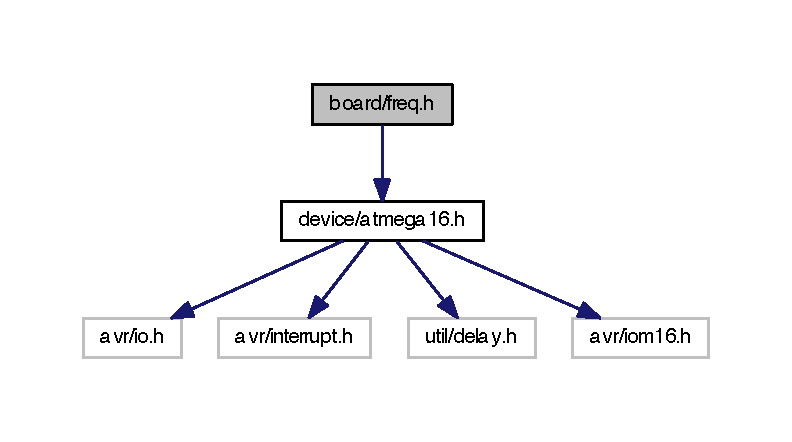
\includegraphics[width=350pt]{freq_8h__incl}
\end{center}
\end{figure}
This graph shows which files directly or indirectly include this file\+:
\nopagebreak
\begin{figure}[H]
\begin{center}
\leavevmode
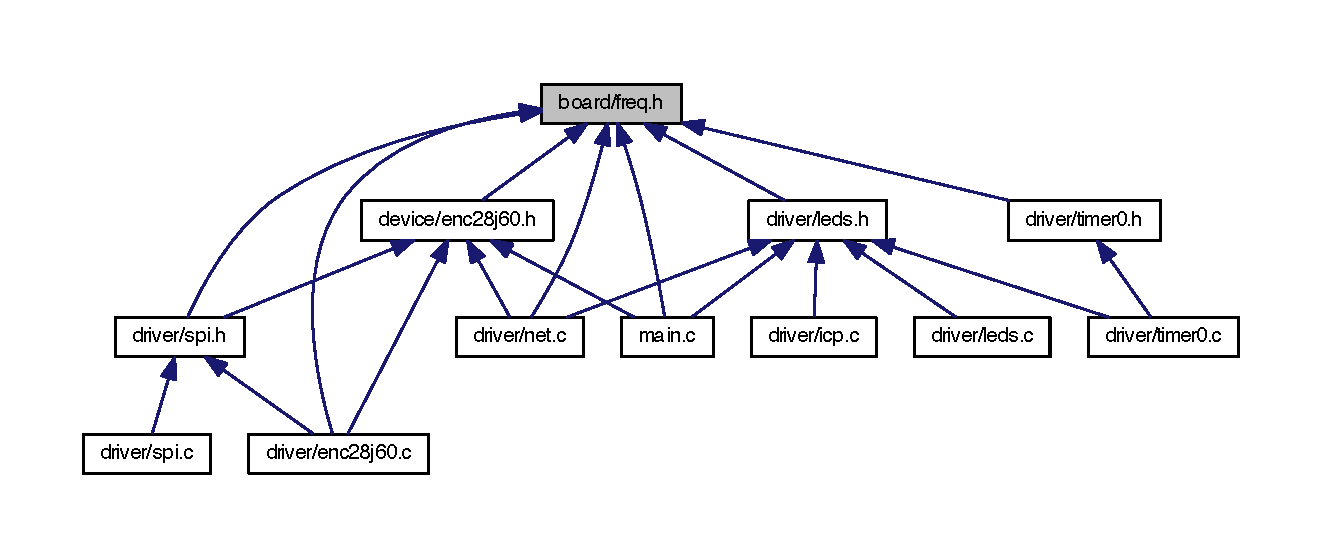
\includegraphics[width=350pt]{freq_8h__dep__incl}
\end{center}
\end{figure}
\subsection*{Macros}
\begin{DoxyCompactItemize}
\item 
\#define \hyperlink{freq_8h_a2eb4252b35effe1188cb61b6124fa617}{L\+E\+D\+\_\+\+D\+D\+R}~D\+D\+R\+A
\item 
\#define \hyperlink{freq_8h_a663daa01e565aee93c6f20c5845b90b4}{L\+E\+D\+\_\+\+P\+O\+R\+T}~P\+O\+R\+T\+A
\item 
\#define \hyperlink{freq_8h_ab4553be4db9860d940f81d7447173b2f}{L\+E\+D\+\_\+\+P\+I\+N}~P\+I\+N\+A
\item 
\#define \hyperlink{freq_8h_ae8d5b4e7e2d9d21caaa4744d385d7cc7}{L\+E\+D0}~P\+A0
\item 
\#define \hyperlink{freq_8h_a8aa85ae9867fabf70ec72cd3bf6fb6b9}{L\+E\+D1}~P\+A1
\item 
\#define \hyperlink{freq_8h_ad09fe5bf321b9a2de26bd5e5b9af6424}{L\+E\+D2}~P\+A2
\item 
\#define \hyperlink{freq_8h_a4b7ff8e253a7412f83deba3a447028a8}{L\+E\+D3}~P\+A3
\item 
\#define \hyperlink{freq_8h_ae048837f20072bed467332b1bd1da9fa}{L\+E\+D4}~P\+A4
\item 
\#define \hyperlink{freq_8h_aefae505e2588183f1921a9e840b16044}{L\+E\+D5}~P\+A5
\item 
\#define \hyperlink{freq_8h_ab922b15d42b90025c9e13c087d86ce81}{L\+E\+D6}~P\+A6
\item 
\#define \hyperlink{freq_8h_a35bf8e7b8f9e9257ca184bbe0c95e929}{L\+E\+D7}~P\+A7
\item 
\#define \hyperlink{freq_8h_ab7100c807e8c6a90956cf37e07d1ffc8}{L\+E\+D\+\_\+\+A\+L\+L}~0x\+F\+F
\item 
\#define \hyperlink{freq_8h_a80700bb63bd56ebabbb4728aa433fd29}{L\+E\+D\+\_\+\+O\+F\+F}~0x00
\item 
\#define \hyperlink{freq_8h_a8b07abe3c166558485851f24f2141dc9}{S\+P\+I\+\_\+\+D\+D\+R}~D\+D\+R\+B
\item 
\#define \hyperlink{freq_8h_a8112c985f7444e82198d7571ce0a9160}{S\+P\+I\+\_\+\+P\+O\+R\+T}~P\+O\+R\+T\+B
\item 
\#define \hyperlink{freq_8h_a81f0aae3c3a2adba06ac3b802b38915a}{S\+P\+I\+\_\+\+S\+S}~P\+B4
\item 
\#define \hyperlink{freq_8h_a7dbebab5f7dd57885adccf6711b13592}{S\+P\+I\+\_\+\+M\+O\+S\+I}~P\+B5
\item 
\#define \hyperlink{freq_8h_ab142cc77dfa97010c9d2b616d0992b64}{S\+P\+I\+\_\+\+M\+I\+S\+O}~P\+B6
\item 
\#define \hyperlink{freq_8h_a750ca7c9b92cfc9e57272ff3a49db48b}{S\+P\+I\+\_\+\+S\+C\+K}~P\+B7
\item 
\#define \hyperlink{freq_8h_a44ac214864a1f7ade32daf7ab95750ec}{E\+N\+C\+\_\+\+C\+T\+R\+L\+\_\+\+D\+D\+R}~D\+D\+R\+B
\item 
\#define \hyperlink{freq_8h_aa0e073dfe978a7f7110e19d9e6c8ab81}{E\+N\+C\+\_\+\+C\+T\+R\+L\+\_\+\+P\+O\+R\+T}~P\+O\+R\+T\+B
\item 
\#define \hyperlink{freq_8h_a6510399fc27f848237a75e87e3ce7a8e}{E\+N\+C\+\_\+\+C\+T\+R\+L\+\_\+\+C\+S}~P\+B3
\end{DoxyCompactItemize}


\subsection{Detailed Description}
pin locations for \char`\"{}\+Frequenzmessung-\/\+Board\char`\"{} 

\begin{DoxyAuthor}{Author}
M. Ozgan, \href{mailto:mozgan@mozgan.org}{\tt mozgan@mozgan.\+org} 
\end{DoxyAuthor}
\begin{DoxyVersion}{Version}
0.\+2 
\end{DoxyVersion}
\begin{DoxyDate}{Date}
19.\+08.\+2013 15\+:13\+:45 
\end{DoxyDate}
\begin{DoxyParagraph}{Compiler}
gcc (on Mac, G\+N\+U/\+Linux and 4.\+4\+B\+S\+D) 
\end{DoxyParagraph}
\begin{DoxyParagraph}{Company}
T\+U Wien 
\end{DoxyParagraph}


\begin{DoxyRefDesc}{Bug}
\item[\hyperlink{bug__bug000001}{Bug}]none \end{DoxyRefDesc}
\begin{DoxyRefDesc}{Todo}
\item[\hyperlink{todo__todo000001}{Todo}]none \end{DoxyRefDesc}


Definition in file \hyperlink{freq_8h_source}{freq.\+h}.



\subsection{Macro Definition Documentation}
\hypertarget{freq_8h_a6510399fc27f848237a75e87e3ce7a8e}{\index{freq.\+h@{freq.\+h}!E\+N\+C\+\_\+\+C\+T\+R\+L\+\_\+\+C\+S@{E\+N\+C\+\_\+\+C\+T\+R\+L\+\_\+\+C\+S}}
\index{E\+N\+C\+\_\+\+C\+T\+R\+L\+\_\+\+C\+S@{E\+N\+C\+\_\+\+C\+T\+R\+L\+\_\+\+C\+S}!freq.\+h@{freq.\+h}}
\subsubsection[{E\+N\+C\+\_\+\+C\+T\+R\+L\+\_\+\+C\+S}]{\setlength{\rightskip}{0pt plus 5cm}\#define E\+N\+C\+\_\+\+C\+T\+R\+L\+\_\+\+C\+S~P\+B3}}\label{freq_8h_a6510399fc27f848237a75e87e3ce7a8e}


Definition at line 60 of file freq.\+h.



Referenced by enc\+\_\+init(), enc\+\_\+start(), and enc\+\_\+stop().

\hypertarget{freq_8h_a44ac214864a1f7ade32daf7ab95750ec}{\index{freq.\+h@{freq.\+h}!E\+N\+C\+\_\+\+C\+T\+R\+L\+\_\+\+D\+D\+R@{E\+N\+C\+\_\+\+C\+T\+R\+L\+\_\+\+D\+D\+R}}
\index{E\+N\+C\+\_\+\+C\+T\+R\+L\+\_\+\+D\+D\+R@{E\+N\+C\+\_\+\+C\+T\+R\+L\+\_\+\+D\+D\+R}!freq.\+h@{freq.\+h}}
\subsubsection[{E\+N\+C\+\_\+\+C\+T\+R\+L\+\_\+\+D\+D\+R}]{\setlength{\rightskip}{0pt plus 5cm}\#define E\+N\+C\+\_\+\+C\+T\+R\+L\+\_\+\+D\+D\+R~D\+D\+R\+B}}\label{freq_8h_a44ac214864a1f7ade32daf7ab95750ec}


Definition at line 58 of file freq.\+h.



Referenced by enc\+\_\+init().

\hypertarget{freq_8h_aa0e073dfe978a7f7110e19d9e6c8ab81}{\index{freq.\+h@{freq.\+h}!E\+N\+C\+\_\+\+C\+T\+R\+L\+\_\+\+P\+O\+R\+T@{E\+N\+C\+\_\+\+C\+T\+R\+L\+\_\+\+P\+O\+R\+T}}
\index{E\+N\+C\+\_\+\+C\+T\+R\+L\+\_\+\+P\+O\+R\+T@{E\+N\+C\+\_\+\+C\+T\+R\+L\+\_\+\+P\+O\+R\+T}!freq.\+h@{freq.\+h}}
\subsubsection[{E\+N\+C\+\_\+\+C\+T\+R\+L\+\_\+\+P\+O\+R\+T}]{\setlength{\rightskip}{0pt plus 5cm}\#define E\+N\+C\+\_\+\+C\+T\+R\+L\+\_\+\+P\+O\+R\+T~P\+O\+R\+T\+B}}\label{freq_8h_aa0e073dfe978a7f7110e19d9e6c8ab81}


Definition at line 59 of file freq.\+h.



Referenced by enc\+\_\+init(), enc\+\_\+start(), and enc\+\_\+stop().

\hypertarget{freq_8h_ae8d5b4e7e2d9d21caaa4744d385d7cc7}{\index{freq.\+h@{freq.\+h}!L\+E\+D0@{L\+E\+D0}}
\index{L\+E\+D0@{L\+E\+D0}!freq.\+h@{freq.\+h}}
\subsubsection[{L\+E\+D0}]{\setlength{\rightskip}{0pt plus 5cm}\#define L\+E\+D0~P\+A0}}\label{freq_8h_ae8d5b4e7e2d9d21caaa4744d385d7cc7}


Definition at line 37 of file freq.\+h.

\hypertarget{freq_8h_a8aa85ae9867fabf70ec72cd3bf6fb6b9}{\index{freq.\+h@{freq.\+h}!L\+E\+D1@{L\+E\+D1}}
\index{L\+E\+D1@{L\+E\+D1}!freq.\+h@{freq.\+h}}
\subsubsection[{L\+E\+D1}]{\setlength{\rightskip}{0pt plus 5cm}\#define L\+E\+D1~P\+A1}}\label{freq_8h_a8aa85ae9867fabf70ec72cd3bf6fb6b9}


Definition at line 38 of file freq.\+h.

\hypertarget{freq_8h_ad09fe5bf321b9a2de26bd5e5b9af6424}{\index{freq.\+h@{freq.\+h}!L\+E\+D2@{L\+E\+D2}}
\index{L\+E\+D2@{L\+E\+D2}!freq.\+h@{freq.\+h}}
\subsubsection[{L\+E\+D2}]{\setlength{\rightskip}{0pt plus 5cm}\#define L\+E\+D2~P\+A2}}\label{freq_8h_ad09fe5bf321b9a2de26bd5e5b9af6424}


Definition at line 39 of file freq.\+h.

\hypertarget{freq_8h_a4b7ff8e253a7412f83deba3a447028a8}{\index{freq.\+h@{freq.\+h}!L\+E\+D3@{L\+E\+D3}}
\index{L\+E\+D3@{L\+E\+D3}!freq.\+h@{freq.\+h}}
\subsubsection[{L\+E\+D3}]{\setlength{\rightskip}{0pt plus 5cm}\#define L\+E\+D3~P\+A3}}\label{freq_8h_a4b7ff8e253a7412f83deba3a447028a8}


Definition at line 40 of file freq.\+h.

\hypertarget{freq_8h_ae048837f20072bed467332b1bd1da9fa}{\index{freq.\+h@{freq.\+h}!L\+E\+D4@{L\+E\+D4}}
\index{L\+E\+D4@{L\+E\+D4}!freq.\+h@{freq.\+h}}
\subsubsection[{L\+E\+D4}]{\setlength{\rightskip}{0pt plus 5cm}\#define L\+E\+D4~P\+A4}}\label{freq_8h_ae048837f20072bed467332b1bd1da9fa}


Definition at line 41 of file freq.\+h.

\hypertarget{freq_8h_aefae505e2588183f1921a9e840b16044}{\index{freq.\+h@{freq.\+h}!L\+E\+D5@{L\+E\+D5}}
\index{L\+E\+D5@{L\+E\+D5}!freq.\+h@{freq.\+h}}
\subsubsection[{L\+E\+D5}]{\setlength{\rightskip}{0pt plus 5cm}\#define L\+E\+D5~P\+A5}}\label{freq_8h_aefae505e2588183f1921a9e840b16044}


Definition at line 42 of file freq.\+h.

\hypertarget{freq_8h_ab922b15d42b90025c9e13c087d86ce81}{\index{freq.\+h@{freq.\+h}!L\+E\+D6@{L\+E\+D6}}
\index{L\+E\+D6@{L\+E\+D6}!freq.\+h@{freq.\+h}}
\subsubsection[{L\+E\+D6}]{\setlength{\rightskip}{0pt plus 5cm}\#define L\+E\+D6~P\+A6}}\label{freq_8h_ab922b15d42b90025c9e13c087d86ce81}


Definition at line 43 of file freq.\+h.

\hypertarget{freq_8h_a35bf8e7b8f9e9257ca184bbe0c95e929}{\index{freq.\+h@{freq.\+h}!L\+E\+D7@{L\+E\+D7}}
\index{L\+E\+D7@{L\+E\+D7}!freq.\+h@{freq.\+h}}
\subsubsection[{L\+E\+D7}]{\setlength{\rightskip}{0pt plus 5cm}\#define L\+E\+D7~P\+A7}}\label{freq_8h_a35bf8e7b8f9e9257ca184bbe0c95e929}


Definition at line 44 of file freq.\+h.

\hypertarget{freq_8h_ab7100c807e8c6a90956cf37e07d1ffc8}{\index{freq.\+h@{freq.\+h}!L\+E\+D\+\_\+\+A\+L\+L@{L\+E\+D\+\_\+\+A\+L\+L}}
\index{L\+E\+D\+\_\+\+A\+L\+L@{L\+E\+D\+\_\+\+A\+L\+L}!freq.\+h@{freq.\+h}}
\subsubsection[{L\+E\+D\+\_\+\+A\+L\+L}]{\setlength{\rightskip}{0pt plus 5cm}\#define L\+E\+D\+\_\+\+A\+L\+L~0x\+F\+F}}\label{freq_8h_ab7100c807e8c6a90956cf37e07d1ffc8}


Definition at line 46 of file freq.\+h.



Referenced by leds\+\_\+init(), leds\+\_\+on(), and leds\+\_\+toggle().

\hypertarget{freq_8h_a2eb4252b35effe1188cb61b6124fa617}{\index{freq.\+h@{freq.\+h}!L\+E\+D\+\_\+\+D\+D\+R@{L\+E\+D\+\_\+\+D\+D\+R}}
\index{L\+E\+D\+\_\+\+D\+D\+R@{L\+E\+D\+\_\+\+D\+D\+R}!freq.\+h@{freq.\+h}}
\subsubsection[{L\+E\+D\+\_\+\+D\+D\+R}]{\setlength{\rightskip}{0pt plus 5cm}\#define L\+E\+D\+\_\+\+D\+D\+R~D\+D\+R\+A}}\label{freq_8h_a2eb4252b35effe1188cb61b6124fa617}


Definition at line 33 of file freq.\+h.



Referenced by led\+\_\+init(), and leds\+\_\+init().

\hypertarget{freq_8h_a80700bb63bd56ebabbb4728aa433fd29}{\index{freq.\+h@{freq.\+h}!L\+E\+D\+\_\+\+O\+F\+F@{L\+E\+D\+\_\+\+O\+F\+F}}
\index{L\+E\+D\+\_\+\+O\+F\+F@{L\+E\+D\+\_\+\+O\+F\+F}!freq.\+h@{freq.\+h}}
\subsubsection[{L\+E\+D\+\_\+\+O\+F\+F}]{\setlength{\rightskip}{0pt plus 5cm}\#define L\+E\+D\+\_\+\+O\+F\+F~0x00}}\label{freq_8h_a80700bb63bd56ebabbb4728aa433fd29}


Definition at line 47 of file freq.\+h.



Referenced by leds\+\_\+init(), and leds\+\_\+off().

\hypertarget{freq_8h_ab4553be4db9860d940f81d7447173b2f}{\index{freq.\+h@{freq.\+h}!L\+E\+D\+\_\+\+P\+I\+N@{L\+E\+D\+\_\+\+P\+I\+N}}
\index{L\+E\+D\+\_\+\+P\+I\+N@{L\+E\+D\+\_\+\+P\+I\+N}!freq.\+h@{freq.\+h}}
\subsubsection[{L\+E\+D\+\_\+\+P\+I\+N}]{\setlength{\rightskip}{0pt plus 5cm}\#define L\+E\+D\+\_\+\+P\+I\+N~P\+I\+N\+A}}\label{freq_8h_ab4553be4db9860d940f81d7447173b2f}


Definition at line 35 of file freq.\+h.

\hypertarget{freq_8h_a663daa01e565aee93c6f20c5845b90b4}{\index{freq.\+h@{freq.\+h}!L\+E\+D\+\_\+\+P\+O\+R\+T@{L\+E\+D\+\_\+\+P\+O\+R\+T}}
\index{L\+E\+D\+\_\+\+P\+O\+R\+T@{L\+E\+D\+\_\+\+P\+O\+R\+T}!freq.\+h@{freq.\+h}}
\subsubsection[{L\+E\+D\+\_\+\+P\+O\+R\+T}]{\setlength{\rightskip}{0pt plus 5cm}\#define L\+E\+D\+\_\+\+P\+O\+R\+T~P\+O\+R\+T\+A}}\label{freq_8h_a663daa01e565aee93c6f20c5845b90b4}


Definition at line 34 of file freq.\+h.



Referenced by led\+\_\+init(), led\+\_\+off(), led\+\_\+on(), led\+\_\+toggle(), leds\+\_\+init(), leds\+\_\+off(), leds\+\_\+on(), and leds\+\_\+toggle().

\hypertarget{freq_8h_a8b07abe3c166558485851f24f2141dc9}{\index{freq.\+h@{freq.\+h}!S\+P\+I\+\_\+\+D\+D\+R@{S\+P\+I\+\_\+\+D\+D\+R}}
\index{S\+P\+I\+\_\+\+D\+D\+R@{S\+P\+I\+\_\+\+D\+D\+R}!freq.\+h@{freq.\+h}}
\subsubsection[{S\+P\+I\+\_\+\+D\+D\+R}]{\setlength{\rightskip}{0pt plus 5cm}\#define S\+P\+I\+\_\+\+D\+D\+R~D\+D\+R\+B}}\label{freq_8h_a8b07abe3c166558485851f24f2141dc9}


Definition at line 50 of file freq.\+h.



Referenced by spi\+\_\+init().

\hypertarget{freq_8h_ab142cc77dfa97010c9d2b616d0992b64}{\index{freq.\+h@{freq.\+h}!S\+P\+I\+\_\+\+M\+I\+S\+O@{S\+P\+I\+\_\+\+M\+I\+S\+O}}
\index{S\+P\+I\+\_\+\+M\+I\+S\+O@{S\+P\+I\+\_\+\+M\+I\+S\+O}!freq.\+h@{freq.\+h}}
\subsubsection[{S\+P\+I\+\_\+\+M\+I\+S\+O}]{\setlength{\rightskip}{0pt plus 5cm}\#define S\+P\+I\+\_\+\+M\+I\+S\+O~P\+B6}}\label{freq_8h_ab142cc77dfa97010c9d2b616d0992b64}


Definition at line 54 of file freq.\+h.



Referenced by spi\+\_\+init().

\hypertarget{freq_8h_a7dbebab5f7dd57885adccf6711b13592}{\index{freq.\+h@{freq.\+h}!S\+P\+I\+\_\+\+M\+O\+S\+I@{S\+P\+I\+\_\+\+M\+O\+S\+I}}
\index{S\+P\+I\+\_\+\+M\+O\+S\+I@{S\+P\+I\+\_\+\+M\+O\+S\+I}!freq.\+h@{freq.\+h}}
\subsubsection[{S\+P\+I\+\_\+\+M\+O\+S\+I}]{\setlength{\rightskip}{0pt plus 5cm}\#define S\+P\+I\+\_\+\+M\+O\+S\+I~P\+B5}}\label{freq_8h_a7dbebab5f7dd57885adccf6711b13592}


Definition at line 53 of file freq.\+h.



Referenced by spi\+\_\+init().

\hypertarget{freq_8h_a8112c985f7444e82198d7571ce0a9160}{\index{freq.\+h@{freq.\+h}!S\+P\+I\+\_\+\+P\+O\+R\+T@{S\+P\+I\+\_\+\+P\+O\+R\+T}}
\index{S\+P\+I\+\_\+\+P\+O\+R\+T@{S\+P\+I\+\_\+\+P\+O\+R\+T}!freq.\+h@{freq.\+h}}
\subsubsection[{S\+P\+I\+\_\+\+P\+O\+R\+T}]{\setlength{\rightskip}{0pt plus 5cm}\#define S\+P\+I\+\_\+\+P\+O\+R\+T~P\+O\+R\+T\+B}}\label{freq_8h_a8112c985f7444e82198d7571ce0a9160}


Definition at line 51 of file freq.\+h.



Referenced by spi\+\_\+init().

\hypertarget{freq_8h_a750ca7c9b92cfc9e57272ff3a49db48b}{\index{freq.\+h@{freq.\+h}!S\+P\+I\+\_\+\+S\+C\+K@{S\+P\+I\+\_\+\+S\+C\+K}}
\index{S\+P\+I\+\_\+\+S\+C\+K@{S\+P\+I\+\_\+\+S\+C\+K}!freq.\+h@{freq.\+h}}
\subsubsection[{S\+P\+I\+\_\+\+S\+C\+K}]{\setlength{\rightskip}{0pt plus 5cm}\#define S\+P\+I\+\_\+\+S\+C\+K~P\+B7}}\label{freq_8h_a750ca7c9b92cfc9e57272ff3a49db48b}


Definition at line 55 of file freq.\+h.



Referenced by spi\+\_\+init().

\hypertarget{freq_8h_a81f0aae3c3a2adba06ac3b802b38915a}{\index{freq.\+h@{freq.\+h}!S\+P\+I\+\_\+\+S\+S@{S\+P\+I\+\_\+\+S\+S}}
\index{S\+P\+I\+\_\+\+S\+S@{S\+P\+I\+\_\+\+S\+S}!freq.\+h@{freq.\+h}}
\subsubsection[{S\+P\+I\+\_\+\+S\+S}]{\setlength{\rightskip}{0pt plus 5cm}\#define S\+P\+I\+\_\+\+S\+S~P\+B4}}\label{freq_8h_a81f0aae3c3a2adba06ac3b802b38915a}


Definition at line 52 of file freq.\+h.



Referenced by spi\+\_\+init().


\hypertarget{atmega16_8h}{\section{device/atmega16.h File Reference}
\label{atmega16_8h}\index{device/atmega16.\+h@{device/atmega16.\+h}}
}


specific definitions for A\+T\+Mega16 device  


{\ttfamily \#include $<$avr/io.\+h$>$}\\*
{\ttfamily \#include $<$avr/interrupt.\+h$>$}\\*
{\ttfamily \#include $<$util/delay.\+h$>$}\\*
{\ttfamily \#include $<$avr/iom16.\+h$>$}\\*
Include dependency graph for atmega16.\+h\+:
\nopagebreak
\begin{figure}[H]
\begin{center}
\leavevmode
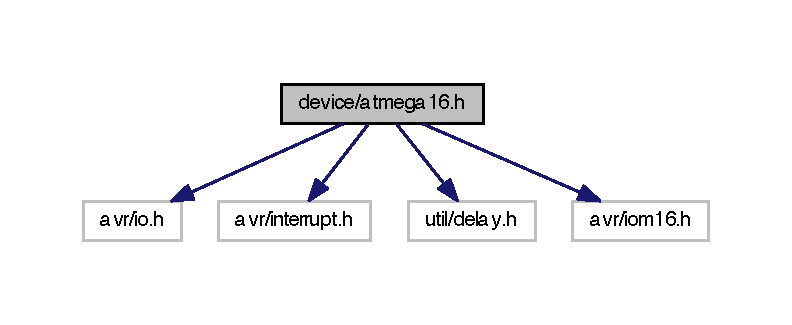
\includegraphics[width=350pt]{atmega16_8h__incl}
\end{center}
\end{figure}
This graph shows which files directly or indirectly include this file\+:
\nopagebreak
\begin{figure}[H]
\begin{center}
\leavevmode
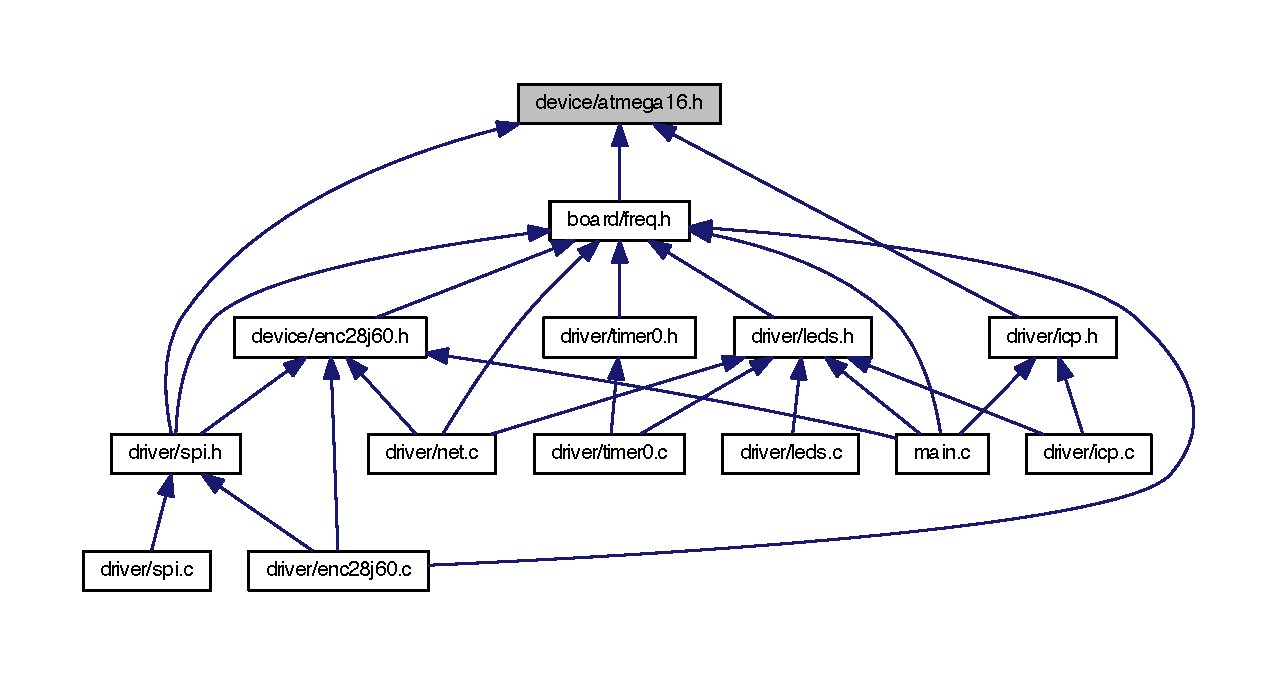
\includegraphics[width=350pt]{atmega16_8h__dep__incl}
\end{center}
\end{figure}
\subsection*{Macros}
\begin{DoxyCompactItemize}
\item 
\#define \hyperlink{atmega16_8h_a43bafb28b29491ec7f871319b5a3b2f8}{F\+\_\+\+C\+P\+U}~16000000		    /$\ast$ C\+P\+U F\+R\+E\+Q\+: 16 M\+Hz $\ast$/
\item 
\#define \hyperlink{atmega16_8h_ab60bfb56cfc56f5d2b84c76246810443}{T\+I\+M\+E\+R\+\_\+\+I\+N\+T\+\_\+\+M\+A\+S\+K}~T\+I\+M\+S\+K
\item 
\#define \hyperlink{atmega16_8h_a859c1254da67c8184cc38f4b39093655}{T\+I\+M\+E\+R\+\_\+\+I\+N\+T\+\_\+\+F\+L\+G}~T\+I\+F\+R
\item 
\#define \hyperlink{atmega16_8h_a45cd53c845ce671ce22fd16f6b4bdf5b}{T\+I\+M\+E\+R0\+\_\+\+C\+N\+T}~T\+C\+N\+T0
\item 
\#define \hyperlink{atmega16_8h_abc62547834bebc4d512d941b8ba557f0}{T\+I\+M\+E\+R0\+\_\+\+O\+C\+R}~O\+C\+R0
\item 
\#define \hyperlink{atmega16_8h_a6d3d80ea887016bf029c90dd78dff20b}{T\+I\+M\+E\+R0\+\_\+\+T\+C\+C\+R}~T\+C\+C\+R0
\item 
\#define \hyperlink{atmega16_8h_a038000b20049a0ae5751c8d01e0bab54}{T\+I\+M\+E\+R0\+\_\+\+N\+O\+\_\+\+C\+L\+K}~(\hyperlink{atmega16_8h_a6d3d80ea887016bf029c90dd78dff20b}{T\+I\+M\+E\+R0\+\_\+\+T\+C\+C\+R} \& 0x\+F8)    /$\ast$($\sim$((1 $<$$<$ C\+S00) $\vert$ (1 $<$$<$ C\+S01) $\vert$ (1 $<$$<$ C\+S02)))$\ast$/
\item 
\#define \hyperlink{atmega16_8h_a1cf4168f3568e5e67474d93fb37ea3ec}{T\+I\+M\+E\+R0\+\_\+\+P\+R\+E\+S\+\_\+1}~(\hyperlink{atmega16_8h_a038000b20049a0ae5751c8d01e0bab54}{T\+I\+M\+E\+R0\+\_\+\+N\+O\+\_\+\+C\+L\+K} $\vert$ (1 $<$$<$ C\+S00))
\item 
\#define \hyperlink{atmega16_8h_a2c470d396b337ee7d58233d268446bf6}{T\+I\+M\+E\+R0\+\_\+\+P\+R\+E\+S\+\_\+8}~(\hyperlink{atmega16_8h_a038000b20049a0ae5751c8d01e0bab54}{T\+I\+M\+E\+R0\+\_\+\+N\+O\+\_\+\+C\+L\+K} $\vert$ (1 $<$$<$ C\+S01))
\item 
\#define \hyperlink{atmega16_8h_a0e7cc469944f4733dc7dfe2656f9c7c0}{T\+I\+M\+E\+R0\+\_\+\+P\+R\+E\+S\+\_\+64}~(\hyperlink{atmega16_8h_a038000b20049a0ae5751c8d01e0bab54}{T\+I\+M\+E\+R0\+\_\+\+N\+O\+\_\+\+C\+L\+K} $\vert$ (1 $<$$<$ C\+S00) $\vert$ (1 $<$$<$ C\+S01))
\item 
\#define \hyperlink{atmega16_8h_a9e32cd2e3d4bf9c7eb33d841b84dcad4}{T\+I\+M\+E\+R0\+\_\+\+P\+R\+E\+S\+\_\+256}~(\hyperlink{atmega16_8h_a038000b20049a0ae5751c8d01e0bab54}{T\+I\+M\+E\+R0\+\_\+\+N\+O\+\_\+\+C\+L\+K} $\vert$ (1 $<$$<$ C\+S02))
\item 
\#define \hyperlink{atmega16_8h_a2e0fe2de7c3e9309053f89b4894b3e3c}{T\+I\+M\+E\+R0\+\_\+\+P\+R\+E\+S\+\_\+1024}~(\hyperlink{atmega16_8h_a038000b20049a0ae5751c8d01e0bab54}{T\+I\+M\+E\+R0\+\_\+\+N\+O\+\_\+\+C\+L\+K} $\vert$ (1 $<$$<$ C\+S00) $\vert$ (1 $<$$<$ C\+S02))
\item 
\#define \hyperlink{atmega16_8h_a59a27e48408600976c04050e9218155c}{T\+I\+M\+E\+R0\+\_\+\+T0\+\_\+\+F\+A\+L\+L}~(\hyperlink{atmega16_8h_a038000b20049a0ae5751c8d01e0bab54}{T\+I\+M\+E\+R0\+\_\+\+N\+O\+\_\+\+C\+L\+K} $\vert$ (1 $<$$<$ C\+S01) $\vert$ (1 $<$$<$ C\+S02))
\item 
\#define \hyperlink{atmega16_8h_a6ccb4eff35040bdfd4191d83921af744}{T\+I\+M\+E\+R0\+\_\+\+T0\+\_\+\+R\+I\+S}~(\hyperlink{atmega16_8h_a038000b20049a0ae5751c8d01e0bab54}{T\+I\+M\+E\+R0\+\_\+\+N\+O\+\_\+\+C\+L\+K} $\vert$ (1 $<$$<$ C\+S00) $\vert$ (1 $<$$<$ C\+S01) $\vert$ (1 $<$$<$ C\+S02))
\item 
\#define \hyperlink{atmega16_8h_a567836f32f69a0f4d9288f51fd2b99c8}{T\+I\+M\+E\+R0\+\_\+\+N\+O\+R\+M\+A\+L\+\_\+\+P}~(\hyperlink{atmega16_8h_a6d3d80ea887016bf029c90dd78dff20b}{T\+I\+M\+E\+R0\+\_\+\+T\+C\+C\+R} \& 0x3\+F)
\item 
\#define \hyperlink{atmega16_8h_afc68168ef4ae73b061158c82ea95c4f6}{T\+I\+M\+E\+R0\+\_\+\+C\+T\+C}~(\hyperlink{atmega16_8h_a567836f32f69a0f4d9288f51fd2b99c8}{T\+I\+M\+E\+R0\+\_\+\+N\+O\+R\+M\+A\+L\+\_\+\+P} $\vert$ (1 $<$$<$ W\+G\+M01))
\item 
\#define \hyperlink{atmega16_8h_a7baedf22cc87698d6a73c7c81c82d468}{T\+I\+M\+E\+R1\+\_\+\+C\+N\+T}~T\+C\+N\+T1
\item 
\#define \hyperlink{atmega16_8h_a017b9946a22770cfe9f686e0348d44e9}{T\+I\+M\+E\+R1\+\_\+\+O\+C\+R\+A}~O\+C\+R1\+A
\item 
\#define \hyperlink{atmega16_8h_a78aaab027e1b02b896861dd14b74171d}{T\+I\+M\+E\+R1\+\_\+\+I\+C\+R}~I\+C\+R1
\item 
\#define \hyperlink{atmega16_8h_a3fa2d3bf1901157f734a584d47b25d8b}{M\+A\+S\+T\+E\+R}~0x01
\item 
\#define \hyperlink{atmega16_8h_ae342da5a4630c191c1c983958808edd8}{S\+L\+A\+V\+E}~0x02
\item 
\#define \hyperlink{atmega16_8h_a4a229380a0f183a9b2aeceb62d06fc91}{S\+P\+I\+\_\+\+D\+A\+T\+A\+\_\+\+R\+E\+G}~S\+P\+D\+R
\item 
\#define \hyperlink{atmega16_8h_ac20c34e07484971a18a665a03b9ce760}{S\+P\+I\+\_\+\+C\+O\+N\+T\+R\+O\+L\+\_\+\+R\+E\+G}~S\+P\+C\+R
\item 
\#define \hyperlink{atmega16_8h_a27537db92d0837cc77baa0d99b8cac48}{S\+P\+I\+\_\+\+E\+N\+A\+B\+L\+E}~S\+P\+E
\item 
\#define \hyperlink{atmega16_8h_afa9464d1e027eef964a5857fe8b90dca}{S\+P\+I\+\_\+\+I\+N\+T\+\_\+\+E\+N\+A\+B\+L\+E}~S\+P\+I\+E
\item 
\#define \hyperlink{atmega16_8h_ae09a2779c2d141aa6a8f8be6d78fe210}{S\+P\+I\+\_\+\+M\+A\+S\+T\+E\+R}~M\+S\+T\+R
\item 
\#define \hyperlink{atmega16_8h_a8d64ca7f86499e5f998ddd2f561901df}{S\+P\+I\+\_\+\+S\+T\+A\+T\+U\+S\+\_\+\+R\+E\+G}~S\+P\+S\+R
\item 
\#define \hyperlink{atmega16_8h_a55d502b0a8f65ab71fb58216a1095e4a}{S\+P\+I\+\_\+\+I\+N\+T\+\_\+\+F\+L\+A\+G}~S\+P\+I\+F
\item 
\#define \hyperlink{atmega16_8h_aa27a35f6b074cbabb8a799183b6429d4}{S\+P\+I\+\_\+\+D\+O\+U\+B\+L\+E\+\_\+\+S\+P\+E\+E\+D}~S\+P\+I2\+X
\end{DoxyCompactItemize}


\subsection{Detailed Description}
specific definitions for A\+T\+Mega16 device 

\begin{DoxyAuthor}{Author}
M. Ozgan, \href{mailto:mozgan@mozgan.org}{\tt mozgan@mozgan.\+org} 
\end{DoxyAuthor}
\begin{DoxyVersion}{Version}
0.\+3 
\end{DoxyVersion}
\begin{DoxyDate}{Date}
19.\+08.\+2013 15\+:18\+:15 
\end{DoxyDate}
\begin{DoxyParagraph}{Compiler}
gcc (on Mac, and 4.\+4\+B\+S\+D) 
\end{DoxyParagraph}
\begin{DoxyParagraph}{Company}
T\+U Wien 
\end{DoxyParagraph}


\begin{DoxyRefDesc}{Bug}
\item[\hyperlink{bug__bug000002}{Bug}]none \end{DoxyRefDesc}
\begin{DoxyRefDesc}{Todo}
\item[\hyperlink{todo__todo000002}{Todo}]none \end{DoxyRefDesc}


Definition in file \hyperlink{atmega16_8h_source}{atmega16.\+h}.



\subsection{Macro Definition Documentation}
\hypertarget{atmega16_8h_a43bafb28b29491ec7f871319b5a3b2f8}{\index{atmega16.\+h@{atmega16.\+h}!F\+\_\+\+C\+P\+U@{F\+\_\+\+C\+P\+U}}
\index{F\+\_\+\+C\+P\+U@{F\+\_\+\+C\+P\+U}!atmega16.\+h@{atmega16.\+h}}
\subsubsection[{F\+\_\+\+C\+P\+U}]{\setlength{\rightskip}{0pt plus 5cm}\#define F\+\_\+\+C\+P\+U~16000000		    /$\ast$ C\+P\+U F\+R\+E\+Q\+: 16 M\+Hz $\ast$/}}\label{atmega16_8h_a43bafb28b29491ec7f871319b5a3b2f8}


Definition at line 42 of file atmega16.\+h.



Referenced by icp\+\_\+init(), main(), and timer0\+\_\+init\+\_\+f().

\hypertarget{atmega16_8h_a3fa2d3bf1901157f734a584d47b25d8b}{\index{atmega16.\+h@{atmega16.\+h}!M\+A\+S\+T\+E\+R@{M\+A\+S\+T\+E\+R}}
\index{M\+A\+S\+T\+E\+R@{M\+A\+S\+T\+E\+R}!atmega16.\+h@{atmega16.\+h}}
\subsubsection[{M\+A\+S\+T\+E\+R}]{\setlength{\rightskip}{0pt plus 5cm}\#define M\+A\+S\+T\+E\+R~0x01}}\label{atmega16_8h_a3fa2d3bf1901157f734a584d47b25d8b}


Definition at line 109 of file atmega16.\+h.

\hypertarget{atmega16_8h_ae342da5a4630c191c1c983958808edd8}{\index{atmega16.\+h@{atmega16.\+h}!S\+L\+A\+V\+E@{S\+L\+A\+V\+E}}
\index{S\+L\+A\+V\+E@{S\+L\+A\+V\+E}!atmega16.\+h@{atmega16.\+h}}
\subsubsection[{S\+L\+A\+V\+E}]{\setlength{\rightskip}{0pt plus 5cm}\#define S\+L\+A\+V\+E~0x02}}\label{atmega16_8h_ae342da5a4630c191c1c983958808edd8}


Definition at line 110 of file atmega16.\+h.

\hypertarget{atmega16_8h_ac20c34e07484971a18a665a03b9ce760}{\index{atmega16.\+h@{atmega16.\+h}!S\+P\+I\+\_\+\+C\+O\+N\+T\+R\+O\+L\+\_\+\+R\+E\+G@{S\+P\+I\+\_\+\+C\+O\+N\+T\+R\+O\+L\+\_\+\+R\+E\+G}}
\index{S\+P\+I\+\_\+\+C\+O\+N\+T\+R\+O\+L\+\_\+\+R\+E\+G@{S\+P\+I\+\_\+\+C\+O\+N\+T\+R\+O\+L\+\_\+\+R\+E\+G}!atmega16.\+h@{atmega16.\+h}}
\subsubsection[{S\+P\+I\+\_\+\+C\+O\+N\+T\+R\+O\+L\+\_\+\+R\+E\+G}]{\setlength{\rightskip}{0pt plus 5cm}\#define S\+P\+I\+\_\+\+C\+O\+N\+T\+R\+O\+L\+\_\+\+R\+E\+G~S\+P\+C\+R}}\label{atmega16_8h_ac20c34e07484971a18a665a03b9ce760}


Definition at line 120 of file atmega16.\+h.



Referenced by spi\+\_\+init().

\hypertarget{atmega16_8h_a4a229380a0f183a9b2aeceb62d06fc91}{\index{atmega16.\+h@{atmega16.\+h}!S\+P\+I\+\_\+\+D\+A\+T\+A\+\_\+\+R\+E\+G@{S\+P\+I\+\_\+\+D\+A\+T\+A\+\_\+\+R\+E\+G}}
\index{S\+P\+I\+\_\+\+D\+A\+T\+A\+\_\+\+R\+E\+G@{S\+P\+I\+\_\+\+D\+A\+T\+A\+\_\+\+R\+E\+G}!atmega16.\+h@{atmega16.\+h}}
\subsubsection[{S\+P\+I\+\_\+\+D\+A\+T\+A\+\_\+\+R\+E\+G}]{\setlength{\rightskip}{0pt plus 5cm}\#define S\+P\+I\+\_\+\+D\+A\+T\+A\+\_\+\+R\+E\+G~S\+P\+D\+R}}\label{atmega16_8h_a4a229380a0f183a9b2aeceb62d06fc91}


Definition at line 112 of file atmega16.\+h.



Referenced by spi\+\_\+write\+\_\+op().

\hypertarget{atmega16_8h_aa27a35f6b074cbabb8a799183b6429d4}{\index{atmega16.\+h@{atmega16.\+h}!S\+P\+I\+\_\+\+D\+O\+U\+B\+L\+E\+\_\+\+S\+P\+E\+E\+D@{S\+P\+I\+\_\+\+D\+O\+U\+B\+L\+E\+\_\+\+S\+P\+E\+E\+D}}
\index{S\+P\+I\+\_\+\+D\+O\+U\+B\+L\+E\+\_\+\+S\+P\+E\+E\+D@{S\+P\+I\+\_\+\+D\+O\+U\+B\+L\+E\+\_\+\+S\+P\+E\+E\+D}!atmega16.\+h@{atmega16.\+h}}
\subsubsection[{S\+P\+I\+\_\+\+D\+O\+U\+B\+L\+E\+\_\+\+S\+P\+E\+E\+D}]{\setlength{\rightskip}{0pt plus 5cm}\#define S\+P\+I\+\_\+\+D\+O\+U\+B\+L\+E\+\_\+\+S\+P\+E\+E\+D~S\+P\+I2\+X}}\label{atmega16_8h_aa27a35f6b074cbabb8a799183b6429d4}


Definition at line 135 of file atmega16.\+h.



Referenced by spi\+\_\+init().

\hypertarget{atmega16_8h_a27537db92d0837cc77baa0d99b8cac48}{\index{atmega16.\+h@{atmega16.\+h}!S\+P\+I\+\_\+\+E\+N\+A\+B\+L\+E@{S\+P\+I\+\_\+\+E\+N\+A\+B\+L\+E}}
\index{S\+P\+I\+\_\+\+E\+N\+A\+B\+L\+E@{S\+P\+I\+\_\+\+E\+N\+A\+B\+L\+E}!atmega16.\+h@{atmega16.\+h}}
\subsubsection[{S\+P\+I\+\_\+\+E\+N\+A\+B\+L\+E}]{\setlength{\rightskip}{0pt plus 5cm}\#define S\+P\+I\+\_\+\+E\+N\+A\+B\+L\+E~S\+P\+E}}\label{atmega16_8h_a27537db92d0837cc77baa0d99b8cac48}


Definition at line 122 of file atmega16.\+h.



Referenced by spi\+\_\+init().

\hypertarget{atmega16_8h_afa9464d1e027eef964a5857fe8b90dca}{\index{atmega16.\+h@{atmega16.\+h}!S\+P\+I\+\_\+\+I\+N\+T\+\_\+\+E\+N\+A\+B\+L\+E@{S\+P\+I\+\_\+\+I\+N\+T\+\_\+\+E\+N\+A\+B\+L\+E}}
\index{S\+P\+I\+\_\+\+I\+N\+T\+\_\+\+E\+N\+A\+B\+L\+E@{S\+P\+I\+\_\+\+I\+N\+T\+\_\+\+E\+N\+A\+B\+L\+E}!atmega16.\+h@{atmega16.\+h}}
\subsubsection[{S\+P\+I\+\_\+\+I\+N\+T\+\_\+\+E\+N\+A\+B\+L\+E}]{\setlength{\rightskip}{0pt plus 5cm}\#define S\+P\+I\+\_\+\+I\+N\+T\+\_\+\+E\+N\+A\+B\+L\+E~S\+P\+I\+E}}\label{atmega16_8h_afa9464d1e027eef964a5857fe8b90dca}


Definition at line 123 of file atmega16.\+h.

\hypertarget{atmega16_8h_a55d502b0a8f65ab71fb58216a1095e4a}{\index{atmega16.\+h@{atmega16.\+h}!S\+P\+I\+\_\+\+I\+N\+T\+\_\+\+F\+L\+A\+G@{S\+P\+I\+\_\+\+I\+N\+T\+\_\+\+F\+L\+A\+G}}
\index{S\+P\+I\+\_\+\+I\+N\+T\+\_\+\+F\+L\+A\+G@{S\+P\+I\+\_\+\+I\+N\+T\+\_\+\+F\+L\+A\+G}!atmega16.\+h@{atmega16.\+h}}
\subsubsection[{S\+P\+I\+\_\+\+I\+N\+T\+\_\+\+F\+L\+A\+G}]{\setlength{\rightskip}{0pt plus 5cm}\#define S\+P\+I\+\_\+\+I\+N\+T\+\_\+\+F\+L\+A\+G~S\+P\+I\+F}}\label{atmega16_8h_a55d502b0a8f65ab71fb58216a1095e4a}


Definition at line 134 of file atmega16.\+h.



Referenced by spi\+\_\+write(), and spi\+\_\+write\+\_\+op().

\hypertarget{atmega16_8h_ae09a2779c2d141aa6a8f8be6d78fe210}{\index{atmega16.\+h@{atmega16.\+h}!S\+P\+I\+\_\+\+M\+A\+S\+T\+E\+R@{S\+P\+I\+\_\+\+M\+A\+S\+T\+E\+R}}
\index{S\+P\+I\+\_\+\+M\+A\+S\+T\+E\+R@{S\+P\+I\+\_\+\+M\+A\+S\+T\+E\+R}!atmega16.\+h@{atmega16.\+h}}
\subsubsection[{S\+P\+I\+\_\+\+M\+A\+S\+T\+E\+R}]{\setlength{\rightskip}{0pt plus 5cm}\#define S\+P\+I\+\_\+\+M\+A\+S\+T\+E\+R~M\+S\+T\+R}}\label{atmega16_8h_ae09a2779c2d141aa6a8f8be6d78fe210}


Definition at line 124 of file atmega16.\+h.



Referenced by spi\+\_\+init().

\hypertarget{atmega16_8h_a8d64ca7f86499e5f998ddd2f561901df}{\index{atmega16.\+h@{atmega16.\+h}!S\+P\+I\+\_\+\+S\+T\+A\+T\+U\+S\+\_\+\+R\+E\+G@{S\+P\+I\+\_\+\+S\+T\+A\+T\+U\+S\+\_\+\+R\+E\+G}}
\index{S\+P\+I\+\_\+\+S\+T\+A\+T\+U\+S\+\_\+\+R\+E\+G@{S\+P\+I\+\_\+\+S\+T\+A\+T\+U\+S\+\_\+\+R\+E\+G}!atmega16.\+h@{atmega16.\+h}}
\subsubsection[{S\+P\+I\+\_\+\+S\+T\+A\+T\+U\+S\+\_\+\+R\+E\+G}]{\setlength{\rightskip}{0pt plus 5cm}\#define S\+P\+I\+\_\+\+S\+T\+A\+T\+U\+S\+\_\+\+R\+E\+G~S\+P\+S\+R}}\label{atmega16_8h_a8d64ca7f86499e5f998ddd2f561901df}


Definition at line 132 of file atmega16.\+h.



Referenced by spi\+\_\+init(), spi\+\_\+write(), and spi\+\_\+write\+\_\+op().

\hypertarget{atmega16_8h_a45cd53c845ce671ce22fd16f6b4bdf5b}{\index{atmega16.\+h@{atmega16.\+h}!T\+I\+M\+E\+R0\+\_\+\+C\+N\+T@{T\+I\+M\+E\+R0\+\_\+\+C\+N\+T}}
\index{T\+I\+M\+E\+R0\+\_\+\+C\+N\+T@{T\+I\+M\+E\+R0\+\_\+\+C\+N\+T}!atmega16.\+h@{atmega16.\+h}}
\subsubsection[{T\+I\+M\+E\+R0\+\_\+\+C\+N\+T}]{\setlength{\rightskip}{0pt plus 5cm}\#define T\+I\+M\+E\+R0\+\_\+\+C\+N\+T~T\+C\+N\+T0}}\label{atmega16_8h_a45cd53c845ce671ce22fd16f6b4bdf5b}


Definition at line 69 of file atmega16.\+h.



Referenced by timer0\+\_\+init\+\_\+f().

\hypertarget{atmega16_8h_afc68168ef4ae73b061158c82ea95c4f6}{\index{atmega16.\+h@{atmega16.\+h}!T\+I\+M\+E\+R0\+\_\+\+C\+T\+C@{T\+I\+M\+E\+R0\+\_\+\+C\+T\+C}}
\index{T\+I\+M\+E\+R0\+\_\+\+C\+T\+C@{T\+I\+M\+E\+R0\+\_\+\+C\+T\+C}!atmega16.\+h@{atmega16.\+h}}
\subsubsection[{T\+I\+M\+E\+R0\+\_\+\+C\+T\+C}]{\setlength{\rightskip}{0pt plus 5cm}\#define T\+I\+M\+E\+R0\+\_\+\+C\+T\+C~({\bf T\+I\+M\+E\+R0\+\_\+\+N\+O\+R\+M\+A\+L\+\_\+\+P} $\vert$ (1 $<$$<$ W\+G\+M01))}}\label{atmega16_8h_afc68168ef4ae73b061158c82ea95c4f6}


Definition at line 96 of file atmega16.\+h.



Referenced by timer0\+\_\+init\+\_\+f().

\hypertarget{atmega16_8h_a038000b20049a0ae5751c8d01e0bab54}{\index{atmega16.\+h@{atmega16.\+h}!T\+I\+M\+E\+R0\+\_\+\+N\+O\+\_\+\+C\+L\+K@{T\+I\+M\+E\+R0\+\_\+\+N\+O\+\_\+\+C\+L\+K}}
\index{T\+I\+M\+E\+R0\+\_\+\+N\+O\+\_\+\+C\+L\+K@{T\+I\+M\+E\+R0\+\_\+\+N\+O\+\_\+\+C\+L\+K}!atmega16.\+h@{atmega16.\+h}}
\subsubsection[{T\+I\+M\+E\+R0\+\_\+\+N\+O\+\_\+\+C\+L\+K}]{\setlength{\rightskip}{0pt plus 5cm}\#define T\+I\+M\+E\+R0\+\_\+\+N\+O\+\_\+\+C\+L\+K~({\bf T\+I\+M\+E\+R0\+\_\+\+T\+C\+C\+R} \& 0x\+F8)    /$\ast$($\sim$((1 $<$$<$ C\+S00) $\vert$ (1 $<$$<$ C\+S01) $\vert$ (1 $<$$<$ C\+S02)))$\ast$/}}\label{atmega16_8h_a038000b20049a0ae5751c8d01e0bab54}


Definition at line 83 of file atmega16.\+h.



Referenced by timer0\+\_\+stop().

\hypertarget{atmega16_8h_a567836f32f69a0f4d9288f51fd2b99c8}{\index{atmega16.\+h@{atmega16.\+h}!T\+I\+M\+E\+R0\+\_\+\+N\+O\+R\+M\+A\+L\+\_\+\+P@{T\+I\+M\+E\+R0\+\_\+\+N\+O\+R\+M\+A\+L\+\_\+\+P}}
\index{T\+I\+M\+E\+R0\+\_\+\+N\+O\+R\+M\+A\+L\+\_\+\+P@{T\+I\+M\+E\+R0\+\_\+\+N\+O\+R\+M\+A\+L\+\_\+\+P}!atmega16.\+h@{atmega16.\+h}}
\subsubsection[{T\+I\+M\+E\+R0\+\_\+\+N\+O\+R\+M\+A\+L\+\_\+\+P}]{\setlength{\rightskip}{0pt plus 5cm}\#define T\+I\+M\+E\+R0\+\_\+\+N\+O\+R\+M\+A\+L\+\_\+\+P~({\bf T\+I\+M\+E\+R0\+\_\+\+T\+C\+C\+R} \& 0x3\+F)}}\label{atmega16_8h_a567836f32f69a0f4d9288f51fd2b99c8}


Definition at line 95 of file atmega16.\+h.

\hypertarget{atmega16_8h_abc62547834bebc4d512d941b8ba557f0}{\index{atmega16.\+h@{atmega16.\+h}!T\+I\+M\+E\+R0\+\_\+\+O\+C\+R@{T\+I\+M\+E\+R0\+\_\+\+O\+C\+R}}
\index{T\+I\+M\+E\+R0\+\_\+\+O\+C\+R@{T\+I\+M\+E\+R0\+\_\+\+O\+C\+R}!atmega16.\+h@{atmega16.\+h}}
\subsubsection[{T\+I\+M\+E\+R0\+\_\+\+O\+C\+R}]{\setlength{\rightskip}{0pt plus 5cm}\#define T\+I\+M\+E\+R0\+\_\+\+O\+C\+R~O\+C\+R0}}\label{atmega16_8h_abc62547834bebc4d512d941b8ba557f0}


Definition at line 70 of file atmega16.\+h.



Referenced by timer0\+\_\+init\+\_\+f().

\hypertarget{atmega16_8h_a1cf4168f3568e5e67474d93fb37ea3ec}{\index{atmega16.\+h@{atmega16.\+h}!T\+I\+M\+E\+R0\+\_\+\+P\+R\+E\+S\+\_\+1@{T\+I\+M\+E\+R0\+\_\+\+P\+R\+E\+S\+\_\+1}}
\index{T\+I\+M\+E\+R0\+\_\+\+P\+R\+E\+S\+\_\+1@{T\+I\+M\+E\+R0\+\_\+\+P\+R\+E\+S\+\_\+1}!atmega16.\+h@{atmega16.\+h}}
\subsubsection[{T\+I\+M\+E\+R0\+\_\+\+P\+R\+E\+S\+\_\+1}]{\setlength{\rightskip}{0pt plus 5cm}\#define T\+I\+M\+E\+R0\+\_\+\+P\+R\+E\+S\+\_\+1~({\bf T\+I\+M\+E\+R0\+\_\+\+N\+O\+\_\+\+C\+L\+K} $\vert$ (1 $<$$<$ C\+S00))}}\label{atmega16_8h_a1cf4168f3568e5e67474d93fb37ea3ec}


Definition at line 84 of file atmega16.\+h.

\hypertarget{atmega16_8h_a2e0fe2de7c3e9309053f89b4894b3e3c}{\index{atmega16.\+h@{atmega16.\+h}!T\+I\+M\+E\+R0\+\_\+\+P\+R\+E\+S\+\_\+1024@{T\+I\+M\+E\+R0\+\_\+\+P\+R\+E\+S\+\_\+1024}}
\index{T\+I\+M\+E\+R0\+\_\+\+P\+R\+E\+S\+\_\+1024@{T\+I\+M\+E\+R0\+\_\+\+P\+R\+E\+S\+\_\+1024}!atmega16.\+h@{atmega16.\+h}}
\subsubsection[{T\+I\+M\+E\+R0\+\_\+\+P\+R\+E\+S\+\_\+1024}]{\setlength{\rightskip}{0pt plus 5cm}\#define T\+I\+M\+E\+R0\+\_\+\+P\+R\+E\+S\+\_\+1024~({\bf T\+I\+M\+E\+R0\+\_\+\+N\+O\+\_\+\+C\+L\+K} $\vert$ (1 $<$$<$ C\+S00) $\vert$ (1 $<$$<$ C\+S02))}}\label{atmega16_8h_a2e0fe2de7c3e9309053f89b4894b3e3c}


Definition at line 88 of file atmega16.\+h.

\hypertarget{atmega16_8h_a9e32cd2e3d4bf9c7eb33d841b84dcad4}{\index{atmega16.\+h@{atmega16.\+h}!T\+I\+M\+E\+R0\+\_\+\+P\+R\+E\+S\+\_\+256@{T\+I\+M\+E\+R0\+\_\+\+P\+R\+E\+S\+\_\+256}}
\index{T\+I\+M\+E\+R0\+\_\+\+P\+R\+E\+S\+\_\+256@{T\+I\+M\+E\+R0\+\_\+\+P\+R\+E\+S\+\_\+256}!atmega16.\+h@{atmega16.\+h}}
\subsubsection[{T\+I\+M\+E\+R0\+\_\+\+P\+R\+E\+S\+\_\+256}]{\setlength{\rightskip}{0pt plus 5cm}\#define T\+I\+M\+E\+R0\+\_\+\+P\+R\+E\+S\+\_\+256~({\bf T\+I\+M\+E\+R0\+\_\+\+N\+O\+\_\+\+C\+L\+K} $\vert$ (1 $<$$<$ C\+S02))}}\label{atmega16_8h_a9e32cd2e3d4bf9c7eb33d841b84dcad4}


Definition at line 87 of file atmega16.\+h.



Referenced by timer0\+\_\+init\+\_\+f().

\hypertarget{atmega16_8h_a0e7cc469944f4733dc7dfe2656f9c7c0}{\index{atmega16.\+h@{atmega16.\+h}!T\+I\+M\+E\+R0\+\_\+\+P\+R\+E\+S\+\_\+64@{T\+I\+M\+E\+R0\+\_\+\+P\+R\+E\+S\+\_\+64}}
\index{T\+I\+M\+E\+R0\+\_\+\+P\+R\+E\+S\+\_\+64@{T\+I\+M\+E\+R0\+\_\+\+P\+R\+E\+S\+\_\+64}!atmega16.\+h@{atmega16.\+h}}
\subsubsection[{T\+I\+M\+E\+R0\+\_\+\+P\+R\+E\+S\+\_\+64}]{\setlength{\rightskip}{0pt plus 5cm}\#define T\+I\+M\+E\+R0\+\_\+\+P\+R\+E\+S\+\_\+64~({\bf T\+I\+M\+E\+R0\+\_\+\+N\+O\+\_\+\+C\+L\+K} $\vert$ (1 $<$$<$ C\+S00) $\vert$ (1 $<$$<$ C\+S01))}}\label{atmega16_8h_a0e7cc469944f4733dc7dfe2656f9c7c0}


Definition at line 86 of file atmega16.\+h.

\hypertarget{atmega16_8h_a2c470d396b337ee7d58233d268446bf6}{\index{atmega16.\+h@{atmega16.\+h}!T\+I\+M\+E\+R0\+\_\+\+P\+R\+E\+S\+\_\+8@{T\+I\+M\+E\+R0\+\_\+\+P\+R\+E\+S\+\_\+8}}
\index{T\+I\+M\+E\+R0\+\_\+\+P\+R\+E\+S\+\_\+8@{T\+I\+M\+E\+R0\+\_\+\+P\+R\+E\+S\+\_\+8}!atmega16.\+h@{atmega16.\+h}}
\subsubsection[{T\+I\+M\+E\+R0\+\_\+\+P\+R\+E\+S\+\_\+8}]{\setlength{\rightskip}{0pt plus 5cm}\#define T\+I\+M\+E\+R0\+\_\+\+P\+R\+E\+S\+\_\+8~({\bf T\+I\+M\+E\+R0\+\_\+\+N\+O\+\_\+\+C\+L\+K} $\vert$ (1 $<$$<$ C\+S01))}}\label{atmega16_8h_a2c470d396b337ee7d58233d268446bf6}


Definition at line 85 of file atmega16.\+h.

\hypertarget{atmega16_8h_a59a27e48408600976c04050e9218155c}{\index{atmega16.\+h@{atmega16.\+h}!T\+I\+M\+E\+R0\+\_\+\+T0\+\_\+\+F\+A\+L\+L@{T\+I\+M\+E\+R0\+\_\+\+T0\+\_\+\+F\+A\+L\+L}}
\index{T\+I\+M\+E\+R0\+\_\+\+T0\+\_\+\+F\+A\+L\+L@{T\+I\+M\+E\+R0\+\_\+\+T0\+\_\+\+F\+A\+L\+L}!atmega16.\+h@{atmega16.\+h}}
\subsubsection[{T\+I\+M\+E\+R0\+\_\+\+T0\+\_\+\+F\+A\+L\+L}]{\setlength{\rightskip}{0pt plus 5cm}\#define T\+I\+M\+E\+R0\+\_\+\+T0\+\_\+\+F\+A\+L\+L~({\bf T\+I\+M\+E\+R0\+\_\+\+N\+O\+\_\+\+C\+L\+K} $\vert$ (1 $<$$<$ C\+S01) $\vert$ (1 $<$$<$ C\+S02))}}\label{atmega16_8h_a59a27e48408600976c04050e9218155c}


Definition at line 89 of file atmega16.\+h.

\hypertarget{atmega16_8h_a6ccb4eff35040bdfd4191d83921af744}{\index{atmega16.\+h@{atmega16.\+h}!T\+I\+M\+E\+R0\+\_\+\+T0\+\_\+\+R\+I\+S@{T\+I\+M\+E\+R0\+\_\+\+T0\+\_\+\+R\+I\+S}}
\index{T\+I\+M\+E\+R0\+\_\+\+T0\+\_\+\+R\+I\+S@{T\+I\+M\+E\+R0\+\_\+\+T0\+\_\+\+R\+I\+S}!atmega16.\+h@{atmega16.\+h}}
\subsubsection[{T\+I\+M\+E\+R0\+\_\+\+T0\+\_\+\+R\+I\+S}]{\setlength{\rightskip}{0pt plus 5cm}\#define T\+I\+M\+E\+R0\+\_\+\+T0\+\_\+\+R\+I\+S~({\bf T\+I\+M\+E\+R0\+\_\+\+N\+O\+\_\+\+C\+L\+K} $\vert$ (1 $<$$<$ C\+S00) $\vert$ (1 $<$$<$ C\+S01) $\vert$ (1 $<$$<$ C\+S02))}}\label{atmega16_8h_a6ccb4eff35040bdfd4191d83921af744}


Definition at line 90 of file atmega16.\+h.

\hypertarget{atmega16_8h_a6d3d80ea887016bf029c90dd78dff20b}{\index{atmega16.\+h@{atmega16.\+h}!T\+I\+M\+E\+R0\+\_\+\+T\+C\+C\+R@{T\+I\+M\+E\+R0\+\_\+\+T\+C\+C\+R}}
\index{T\+I\+M\+E\+R0\+\_\+\+T\+C\+C\+R@{T\+I\+M\+E\+R0\+\_\+\+T\+C\+C\+R}!atmega16.\+h@{atmega16.\+h}}
\subsubsection[{T\+I\+M\+E\+R0\+\_\+\+T\+C\+C\+R}]{\setlength{\rightskip}{0pt plus 5cm}\#define T\+I\+M\+E\+R0\+\_\+\+T\+C\+C\+R~T\+C\+C\+R0}}\label{atmega16_8h_a6d3d80ea887016bf029c90dd78dff20b}


Definition at line 78 of file atmega16.\+h.



Referenced by timer0\+\_\+init\+\_\+f(), and timer0\+\_\+stop().

\hypertarget{atmega16_8h_a7baedf22cc87698d6a73c7c81c82d468}{\index{atmega16.\+h@{atmega16.\+h}!T\+I\+M\+E\+R1\+\_\+\+C\+N\+T@{T\+I\+M\+E\+R1\+\_\+\+C\+N\+T}}
\index{T\+I\+M\+E\+R1\+\_\+\+C\+N\+T@{T\+I\+M\+E\+R1\+\_\+\+C\+N\+T}!atmega16.\+h@{atmega16.\+h}}
\subsubsection[{T\+I\+M\+E\+R1\+\_\+\+C\+N\+T}]{\setlength{\rightskip}{0pt plus 5cm}\#define T\+I\+M\+E\+R1\+\_\+\+C\+N\+T~T\+C\+N\+T1}}\label{atmega16_8h_a7baedf22cc87698d6a73c7c81c82d468}


Definition at line 101 of file atmega16.\+h.

\hypertarget{atmega16_8h_a78aaab027e1b02b896861dd14b74171d}{\index{atmega16.\+h@{atmega16.\+h}!T\+I\+M\+E\+R1\+\_\+\+I\+C\+R@{T\+I\+M\+E\+R1\+\_\+\+I\+C\+R}}
\index{T\+I\+M\+E\+R1\+\_\+\+I\+C\+R@{T\+I\+M\+E\+R1\+\_\+\+I\+C\+R}!atmega16.\+h@{atmega16.\+h}}
\subsubsection[{T\+I\+M\+E\+R1\+\_\+\+I\+C\+R}]{\setlength{\rightskip}{0pt plus 5cm}\#define T\+I\+M\+E\+R1\+\_\+\+I\+C\+R~I\+C\+R1}}\label{atmega16_8h_a78aaab027e1b02b896861dd14b74171d}


Definition at line 103 of file atmega16.\+h.

\hypertarget{atmega16_8h_a017b9946a22770cfe9f686e0348d44e9}{\index{atmega16.\+h@{atmega16.\+h}!T\+I\+M\+E\+R1\+\_\+\+O\+C\+R\+A@{T\+I\+M\+E\+R1\+\_\+\+O\+C\+R\+A}}
\index{T\+I\+M\+E\+R1\+\_\+\+O\+C\+R\+A@{T\+I\+M\+E\+R1\+\_\+\+O\+C\+R\+A}!atmega16.\+h@{atmega16.\+h}}
\subsubsection[{T\+I\+M\+E\+R1\+\_\+\+O\+C\+R\+A}]{\setlength{\rightskip}{0pt plus 5cm}\#define T\+I\+M\+E\+R1\+\_\+\+O\+C\+R\+A~O\+C\+R1\+A}}\label{atmega16_8h_a017b9946a22770cfe9f686e0348d44e9}


Definition at line 102 of file atmega16.\+h.

\hypertarget{atmega16_8h_a859c1254da67c8184cc38f4b39093655}{\index{atmega16.\+h@{atmega16.\+h}!T\+I\+M\+E\+R\+\_\+\+I\+N\+T\+\_\+\+F\+L\+G@{T\+I\+M\+E\+R\+\_\+\+I\+N\+T\+\_\+\+F\+L\+G}}
\index{T\+I\+M\+E\+R\+\_\+\+I\+N\+T\+\_\+\+F\+L\+G@{T\+I\+M\+E\+R\+\_\+\+I\+N\+T\+\_\+\+F\+L\+G}!atmega16.\+h@{atmega16.\+h}}
\subsubsection[{T\+I\+M\+E\+R\+\_\+\+I\+N\+T\+\_\+\+F\+L\+G}]{\setlength{\rightskip}{0pt plus 5cm}\#define T\+I\+M\+E\+R\+\_\+\+I\+N\+T\+\_\+\+F\+L\+G~T\+I\+F\+R}}\label{atmega16_8h_a859c1254da67c8184cc38f4b39093655}


Definition at line 63 of file atmega16.\+h.



Referenced by timer0\+\_\+init\+\_\+f().

\hypertarget{atmega16_8h_ab60bfb56cfc56f5d2b84c76246810443}{\index{atmega16.\+h@{atmega16.\+h}!T\+I\+M\+E\+R\+\_\+\+I\+N\+T\+\_\+\+M\+A\+S\+K@{T\+I\+M\+E\+R\+\_\+\+I\+N\+T\+\_\+\+M\+A\+S\+K}}
\index{T\+I\+M\+E\+R\+\_\+\+I\+N\+T\+\_\+\+M\+A\+S\+K@{T\+I\+M\+E\+R\+\_\+\+I\+N\+T\+\_\+\+M\+A\+S\+K}!atmega16.\+h@{atmega16.\+h}}
\subsubsection[{T\+I\+M\+E\+R\+\_\+\+I\+N\+T\+\_\+\+M\+A\+S\+K}]{\setlength{\rightskip}{0pt plus 5cm}\#define T\+I\+M\+E\+R\+\_\+\+I\+N\+T\+\_\+\+M\+A\+S\+K~T\+I\+M\+S\+K}}\label{atmega16_8h_ab60bfb56cfc56f5d2b84c76246810443}


Definition at line 55 of file atmega16.\+h.



Referenced by timer0\+\_\+init\+\_\+f().


\hypertarget{enc28j60_8h}{\section{device/enc28j60.h File Reference}
\label{enc28j60_8h}\index{device/enc28j60.\+h@{device/enc28j60.\+h}}
}


registers of E\+N\+C28\+J60 device  


{\ttfamily \#include $<$board/freq.\+h$>$}\\*
{\ttfamily \#include $<$include/common.\+h$>$}\\*
{\ttfamily \#include $<$inttypes.\+h$>$}\\*
Include dependency graph for enc28j60.\+h\+:
\nopagebreak
\begin{figure}[H]
\begin{center}
\leavevmode
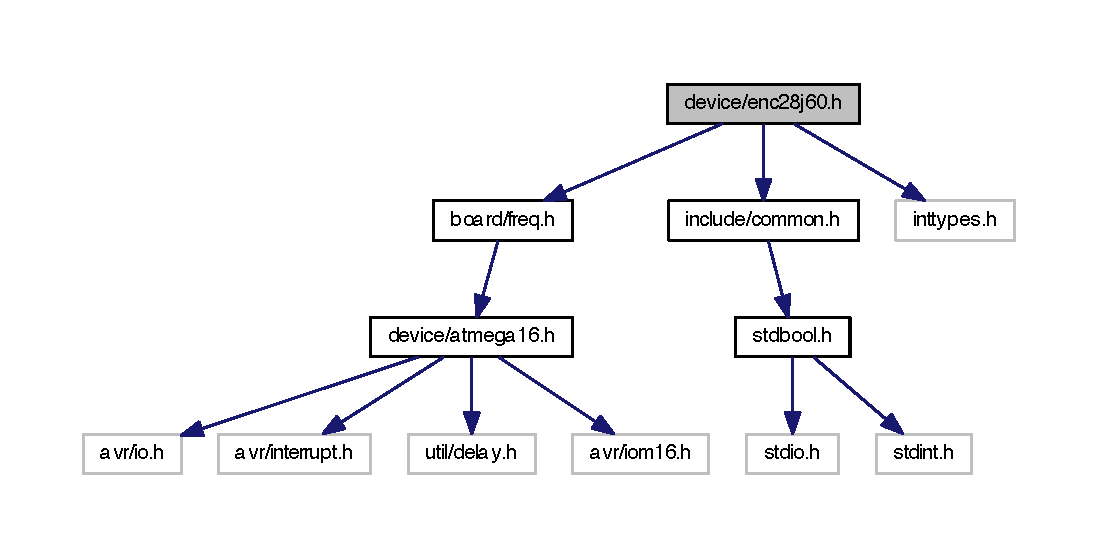
\includegraphics[width=350pt]{enc28j60_8h__incl}
\end{center}
\end{figure}
This graph shows which files directly or indirectly include this file\+:
\nopagebreak
\begin{figure}[H]
\begin{center}
\leavevmode
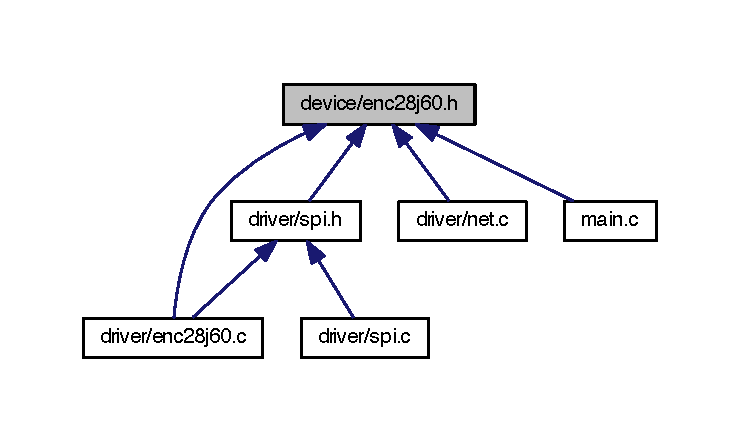
\includegraphics[width=350pt]{enc28j60_8h__dep__incl}
\end{center}
\end{figure}
\subsection*{Macros}
\begin{DoxyCompactItemize}
\item 
\#define \hyperlink{enc28j60_8h_a15b16c1073c60f0be255caf0a60251be}{A\+D\+D\+R\+\_\+\+M\+A\+S\+K}~0x1\+F
\item 
\#define \hyperlink{enc28j60_8h_ac60597badc76e6f2c5ce64d862746c67}{B\+A\+N\+K\+\_\+\+M\+A\+S\+K}~0x60
\item 
\#define \hyperlink{enc28j60_8h_af95ee1390b9678f34abf0c4e19bfb051}{S\+P\+R\+D\+\_\+\+M\+A\+S\+K}~0x80
\item 
\#define \hyperlink{enc28j60_8h_a72ac42db94893a565a52821f5ae95856}{E\+I\+E}~0x1\+B
\item 
\#define \hyperlink{enc28j60_8h_a43a65160b20f5e730c46db801286999a}{I\+N\+T\+I\+E}~0x80
\item 
\#define \hyperlink{enc28j60_8h_a53aa835c371385eab675a3a582a8ba2d}{P\+K\+T\+I\+E}~0x40
\item 
\#define \hyperlink{enc28j60_8h_a6b8293f220c6dcf823b6d8220562b81e}{D\+M\+A\+I\+E}~0x20
\item 
\#define \hyperlink{enc28j60_8h_a1904f4ac5f3a38c3f32feea615ab44e2}{L\+I\+N\+K\+I\+E}~0x10
\item 
\#define \hyperlink{enc28j60_8h_af85ac7f4899bd56c36ed2a0ca53df422}{T\+X\+I\+E}~0x08
\item 
\#define \hyperlink{enc28j60_8h_a0ac64e1af64188179c8ebe57cb882fff}{E\+I\+E\+\_\+\+W\+O\+L\+I\+E}~0x04
\item 
\#define \hyperlink{enc28j60_8h_ac2f309bd5f52f64ecbb04e394b834a44}{T\+X\+E\+R\+I\+E}~0x02
\item 
\#define \hyperlink{enc28j60_8h_ad13655c69641fe3b2c0cc90fd3d42084}{R\+X\+E\+R\+I\+E}~0x01
\item 
\#define \hyperlink{enc28j60_8h_a303aba585a8da3f8dc80315dc94cb0e5}{E\+I\+R}~0x1\+C
\item 
\#define \hyperlink{enc28j60_8h_a567e73e06d0b2569df3aa2c53c4540bb}{P\+K\+T\+I\+F}~0x40
\item 
\#define \hyperlink{enc28j60_8h_a706233f0bf7e747aaf1d08be4f37d233}{D\+M\+A\+I\+F}~0x20
\item 
\#define \hyperlink{enc28j60_8h_a19701d42e07672f373b42b235e30a6ea}{L\+I\+N\+K\+I\+F}~0x10
\item 
\#define \hyperlink{enc28j60_8h_ac765fb3c77a3c11ddd4e7ac9ea7b4bed}{T\+X\+I\+F}~0x08
\item 
\#define \hyperlink{enc28j60_8h_a93413173c7231eb9d949db8f2018608e}{E\+I\+R\+\_\+\+W\+O\+L\+I\+F}~0x04
\item 
\#define \hyperlink{enc28j60_8h_a7a0f9cb1aef73f027e31bd01426f2d7a}{T\+X\+E\+R\+I\+F}~0x02
\item 
\#define \hyperlink{enc28j60_8h_adb3411c72b313ba961c0cf775cf9db02}{R\+X\+E\+R\+I\+F}~0x01
\item 
\#define \hyperlink{enc28j60_8h_ad05043a04b51b3953259c24040e2e99f}{E\+S\+T\+A\+T}~0x1\+D
\item 
\#define \hyperlink{enc28j60_8h_afeeffe52c8fd59db7c61cf8b02042dbf}{I\+N\+T}~0x80
\item 
\#define \hyperlink{enc28j60_8h_a6e7f68840c27418fc87dd0be1bfb21f3}{B\+U\+F\+E\+R}~0x40
\item 
\#define \hyperlink{enc28j60_8h_a9058dd6a31f3b04d9c4ad81a6280793f}{E\+S\+T\+A\+T\+\_\+\+R}~0x20
\item 
\#define \hyperlink{enc28j60_8h_afde62340528064ffed7b85d4a044426b}{L\+A\+T\+E\+C\+O\+L}~0x10
\item 
\#define \hyperlink{enc28j60_8h_adc44bbf15dfbdb380389cef57af88b6d}{R\+X\+B\+U\+S\+Y}~0x04
\item 
\#define \hyperlink{enc28j60_8h_a772c979aff8b1cfc6d64612c7b6d1a73}{T\+X\+A\+B\+R\+T}~0x02
\item 
\#define \hyperlink{enc28j60_8h_ab8108f29c6eb17edb95d8e3e86269ae2}{C\+L\+K\+R\+D\+Y}~0x01
\item 
\#define \hyperlink{enc28j60_8h_a86d77e305cc8d23f335fb733870a873c}{E\+C\+O\+N2}~0x1\+E
\item 
\#define \hyperlink{enc28j60_8h_aa9c885d30bc1d99229e0cd88766799d0}{A\+U\+T\+O\+I\+N\+C}~0x80
\item 
\#define \hyperlink{enc28j60_8h_a2749c0d85a8e2a2686eb6c05ccae2087}{P\+K\+T\+D\+E\+C}~0x40
\item 
\#define \hyperlink{enc28j60_8h_a1cccb4a1ed06b0b6f0fb15f586a6e907}{P\+W\+R\+S\+V}~0x20
\item 
\#define \hyperlink{enc28j60_8h_ada0a40b35b71cc4b342ef240dd0fbc59}{E\+C\+O\+N2\+\_\+\+R}~0x10
\item 
\#define \hyperlink{enc28j60_8h_adcc697ac647d091ace83a79ec0df74c0}{V\+R\+P\+F}~0x08
\item 
\#define \hyperlink{enc28j60_8h_a461b29cd8a06dc2f331f664eb0f9165a}{E\+C\+O\+N1}~0x1\+F
\item 
\#define \hyperlink{enc28j60_8h_a24074ab99aa1bbaa1c6ea4cca511f3ef}{T\+X\+R\+S\+T}~0x80
\item 
\#define \hyperlink{enc28j60_8h_ad1aa5e4bcaed448c4d161b97b8ac1282}{R\+X\+R\+S\+T}~0x40
\item 
\#define \hyperlink{enc28j60_8h_a0cc14b13f53f941a87199fd98de97df7}{D\+M\+A\+S\+T}~0x20
\item 
\#define \hyperlink{enc28j60_8h_a09feccd25a7f699bf70204cd868a35e8}{C\+S\+U\+M\+E\+N}~0x10
\item 
\#define \hyperlink{enc28j60_8h_ac97c83c67cb160908e4f640370155c2a}{T\+X\+R\+T\+S}~0x08
\item 
\#define \hyperlink{enc28j60_8h_a92d07eb614520d8f8d7a5c9b76803582}{E\+\_\+\+R\+X\+E\+N}~0x04
\item 
\#define \hyperlink{enc28j60_8h_a13585e5eab60890dea97428a87aaedb8}{B\+S\+E\+L1}~0x02
\item 
\#define \hyperlink{enc28j60_8h_a1320d47d304bce64ebb5494c1538a220}{B\+S\+E\+L0}~0x01
\item 
\#define \hyperlink{enc28j60_8h_a4a7bf3d4c8a72b0e09ffd6f866ae60f9}{B\+A\+N\+K0}~(0x00)
\item 
\#define \hyperlink{enc28j60_8h_a04e5f3a270ebf2b1a1121b38fef2a62e}{E\+R\+D\+P\+T\+L}~(0x00 $\vert$ B\+A\+N\+K0)
\item 
\#define \hyperlink{enc28j60_8h_a63011487c82b6f6d1fcc749b55e5511e}{E\+R\+D\+P\+T\+H}~(0x01 $\vert$ B\+A\+N\+K0)
\item 
\#define \hyperlink{enc28j60_8h_a684dfa8cb9097ee131a2c9d2ee65d573}{E\+W\+R\+P\+T\+L}~(0x02 $\vert$ B\+A\+N\+K0)
\item 
\#define \hyperlink{enc28j60_8h_a7bda37d486623efbe3ac2055198d356a}{E\+W\+R\+P\+T\+H}~(0x03 $\vert$ B\+A\+N\+K0)
\item 
\#define \hyperlink{enc28j60_8h_a45a38712c4d618bb5cb013e3d781db46}{E\+T\+X\+S\+T\+L}~(0x04 $\vert$ B\+A\+N\+K0)
\item 
\#define \hyperlink{enc28j60_8h_adfc695618aa5a32160cc9e2b0234c714}{E\+T\+X\+S\+T\+H}~(0x05 $\vert$ B\+A\+N\+K0)
\item 
\#define \hyperlink{enc28j60_8h_ad79a19cc60b7dc19cec9df691e658714}{E\+T\+X\+N\+D\+L}~(0x06 $\vert$ B\+A\+N\+K0)
\item 
\#define \hyperlink{enc28j60_8h_a24597e8d914818adae20bf39c4ac7d0e}{E\+T\+X\+N\+D\+H}~(0x07 $\vert$ B\+A\+N\+K0)
\item 
\#define \hyperlink{enc28j60_8h_a387e1ac675539e1c0c7f158f59eafd51}{E\+R\+X\+S\+T\+L}~(0x08 $\vert$ B\+A\+N\+K0)
\item 
\#define \hyperlink{enc28j60_8h_ad4c2a40d74ded1e155f7eb18effb76ba}{E\+R\+X\+S\+T\+H}~(0x09 $\vert$ B\+A\+N\+K0)
\item 
\#define \hyperlink{enc28j60_8h_a9fa6592ccdfa66aa5a1854dd95b6329c}{E\+R\+X\+N\+D\+L}~(0x0\+A $\vert$ B\+A\+N\+K0)
\item 
\#define \hyperlink{enc28j60_8h_a19ee05a22525dcd9e4124734a3aec1b0}{E\+R\+X\+N\+D\+H}~(0x0\+B $\vert$ B\+A\+N\+K0)
\item 
\#define \hyperlink{enc28j60_8h_a0e4345b59cc531bd8daee2cd8c8e906b}{E\+R\+X\+R\+D\+P\+T\+L}~(0x0\+C $\vert$ B\+A\+N\+K0)
\item 
\#define \hyperlink{enc28j60_8h_a1668b845f0bc37dbb515c2358357a690}{E\+R\+X\+R\+D\+P\+T\+H}~(0x0\+D $\vert$ B\+A\+N\+K0)
\item 
\#define \hyperlink{enc28j60_8h_a7d78e648da085c6fdf006d75b3c99a7a}{E\+R\+X\+W\+R\+P\+T\+L}~(0x0\+E $\vert$ B\+A\+N\+K0)
\item 
\#define \hyperlink{enc28j60_8h_a9c9ff6952a5cb0c0b420bc6a405d726c}{E\+R\+X\+W\+R\+P\+T\+H}~(0x0\+F $\vert$ B\+A\+N\+K0)
\item 
\#define \hyperlink{enc28j60_8h_ae7f7aba80e78f4086dc761608c2da2c4}{E\+D\+M\+A\+S\+T\+L}~(0x10 $\vert$ B\+A\+N\+K0)
\item 
\#define \hyperlink{enc28j60_8h_a0b279b45e0cfbc32896ec3b68694cf71}{E\+D\+M\+A\+S\+T\+H}~(0x11 $\vert$ B\+A\+N\+K0)
\item 
\#define \hyperlink{enc28j60_8h_a2138d173a354731c15f3ae6ce5d02b56}{E\+D\+M\+A\+N\+D\+L}~(0x12 $\vert$ B\+A\+N\+K0)
\item 
\#define \hyperlink{enc28j60_8h_ac8866e9f637f6349bb28c6d9152ad658}{E\+D\+M\+A\+N\+D\+H}~(0x13 $\vert$ B\+A\+N\+K0)
\item 
\#define \hyperlink{enc28j60_8h_a6959cbf10d897b0eac13a15928f87cac}{E\+D\+M\+A\+D\+S\+T\+L}~(0x14 $\vert$ B\+A\+N\+K0)
\item 
\#define \hyperlink{enc28j60_8h_ab24279deee959774407b010264cb700a}{E\+D\+M\+A\+D\+S\+T\+H}~(0x15 $\vert$ B\+A\+N\+K0)
\item 
\#define \hyperlink{enc28j60_8h_a9008ca9117933ffaed4f71a0c467ae07}{E\+D\+M\+A\+C\+S\+L}~(0x16 $\vert$ B\+A\+N\+K0)
\item 
\#define \hyperlink{enc28j60_8h_a8db6aa7fd9a0f04a045c04f67523621d}{E\+D\+M\+A\+C\+S\+H}~(0x17 $\vert$ B\+A\+N\+K0)
\item 
\#define \hyperlink{enc28j60_8h_a8d7bd7d547b12ee3c6a267ad57ab46d3}{B\+A\+N\+K1}~(0x20)
\item 
\#define \hyperlink{enc28j60_8h_ad1d8a24d50000168964dc660074bf044}{E\+H\+T0}~(0x00 $\vert$ B\+A\+N\+K1)
\item 
\#define \hyperlink{enc28j60_8h_acf17605d4551244f07220b4fdf778b38}{E\+H\+T1}~(0x01 $\vert$ B\+A\+N\+K1)
\item 
\#define \hyperlink{enc28j60_8h_a2e1a60e1a93a4e6f288d89c825ff1f26}{E\+H\+T2}~(0x02 $\vert$ B\+A\+N\+K1)
\item 
\#define \hyperlink{enc28j60_8h_a1644d7f0cca924f726f81a03423eded6}{E\+H\+T3}~(0x03 $\vert$ B\+A\+N\+K1)
\item 
\#define \hyperlink{enc28j60_8h_ad983f328c5a5606195cdf5ace8768335}{E\+H\+T4}~(0x04 $\vert$ B\+A\+N\+K1)
\item 
\#define \hyperlink{enc28j60_8h_a2788e2e180096007012a6eb7cf6ec951}{E\+H\+T5}~(0x05 $\vert$ B\+A\+N\+K1)
\item 
\#define \hyperlink{enc28j60_8h_a4eb1b56144bc6cf300486b8e6da871d3}{E\+H\+T6}~(0x06 $\vert$ B\+A\+N\+K1)
\item 
\#define \hyperlink{enc28j60_8h_a469059ed79caab2c9733f6044a318d3f}{E\+H\+T7}~(0x07 $\vert$ B\+A\+N\+K1)
\item 
\#define \hyperlink{enc28j60_8h_a7231ae8160a585d71a3e96d93358970c}{E\+P\+M\+M0}~(0x08 $\vert$ B\+A\+N\+K1)
\item 
\#define \hyperlink{enc28j60_8h_a1a0b4ba274784466f2094833facc6792}{E\+P\+M\+M1}~(0x09 $\vert$ B\+A\+N\+K1)
\item 
\#define \hyperlink{enc28j60_8h_a045c306adf0b93289ad90721439ff811}{E\+P\+M\+M2}~(0x0\+A $\vert$ B\+A\+N\+K1)
\item 
\#define \hyperlink{enc28j60_8h_af60e219282fed81ae6e08fb65aad48dc}{E\+P\+M\+M3}~(0x0\+B $\vert$ B\+A\+N\+K1)
\item 
\#define \hyperlink{enc28j60_8h_acc1614ff436a3aee2b85320db84d28ba}{E\+P\+M\+M4}~(0x0\+C $\vert$ B\+A\+N\+K1)
\item 
\#define \hyperlink{enc28j60_8h_ad2c168fc15ba3b06d8ebbf0713ed9e6b}{E\+P\+M\+M5}~(0x0\+D $\vert$ B\+A\+N\+K1)
\item 
\#define \hyperlink{enc28j60_8h_a8300c5c4aa4c2296ea27686c149006d6}{E\+P\+M\+M6}~(0x0\+E $\vert$ B\+A\+N\+K1)
\item 
\#define \hyperlink{enc28j60_8h_aabe6953f6fb64613948c418b1764dc20}{E\+P\+M\+M7}~(0x0\+F $\vert$ B\+A\+N\+K1)
\item 
\#define \hyperlink{enc28j60_8h_a63e21e6d3b5926b59207f79ff66f977d}{E\+P\+M\+C\+S\+L}~(0x10 $\vert$ B\+A\+N\+K1)
\item 
\#define \hyperlink{enc28j60_8h_aea835cc109c3eb4cfedc6f3ad4d7c410}{E\+P\+M\+C\+S\+H}~(0x11 $\vert$ B\+A\+N\+K1)
\item 
\#define \hyperlink{enc28j60_8h_aef01aecd2f0097fc30bf29fe24ab1d05}{E\+P\+M\+O\+L}~(0x14 $\vert$ B\+A\+N\+K1)
\item 
\#define \hyperlink{enc28j60_8h_a432a59eb0f0ccd8d231c82b039dc113d}{E\+P\+M\+O\+H}~(0x15 $\vert$ B\+A\+N\+K1)
\item 
\#define \hyperlink{enc28j60_8h_ab7da9e76b01d840f66c49ae0cdcb91f9}{E\+W\+O\+L\+I\+E}~(0x16 $\vert$ B\+A\+N\+K1)
\item 
\#define \hyperlink{enc28j60_8h_a2e40c6ad151e1b77b892b538ff3ea98f}{E\+W\+O\+L\+I\+R}~(0x17 $\vert$ B\+A\+N\+K1)
\item 
\#define \hyperlink{enc28j60_8h_ac5ff36d9b43977e5dd6548170ec93ddc}{E\+R\+X\+F\+C\+O\+N}~(0x18 $\vert$ B\+A\+N\+K1)
\item 
\#define \hyperlink{enc28j60_8h_a029f8b5f05e4e5182aa9a73e31c4a4f0}{E\+P\+K\+T\+C\+N\+T}~(0x19 $\vert$ B\+A\+N\+K1)
\item 
\#define \hyperlink{enc28j60_8h_a0bd289e48aaf00c5d668738b94c0ddf4}{B\+A\+N\+K2}~(0x40)
\item 
\#define \hyperlink{enc28j60_8h_ab64add14e73a7308bd32343c45caf79d}{M\+A\+C\+O\+N1}~(0x00 $\vert$ B\+A\+N\+K2 $\vert$ 0x80)
\item 
\#define \hyperlink{enc28j60_8h_a01501b400de6174cd44cd52cf9da0950}{M\+A\+C\+O\+N2}~(0x01 $\vert$ B\+A\+N\+K2 $\vert$ 0x80)
\item 
\#define \hyperlink{enc28j60_8h_a37e80f66673c39e7db383e0b11a159ea}{M\+A\+C\+O\+N3}~(0x02 $\vert$ B\+A\+N\+K2 $\vert$ 0x80)
\item 
\#define \hyperlink{enc28j60_8h_a53c0d8f74a3ba17d1337e297ef749a22}{M\+A\+C\+O\+N4}~(0x03 $\vert$ B\+A\+N\+K2 $\vert$ 0x80)
\item 
\#define \hyperlink{enc28j60_8h_a0aa3bb65f69bc921f3b4020410f7efc2}{M\+A\+B\+B\+I\+P\+G}~(0x04 $\vert$ B\+A\+N\+K2 $\vert$ 0x80)
\item 
\#define \hyperlink{enc28j60_8h_a8daa7f7ef529828ef4cc3d90a48ff730}{M\+A\+I\+P\+G\+L}~(0x06 $\vert$ B\+A\+N\+K2 $\vert$ 0x80)
\item 
\#define \hyperlink{enc28j60_8h_a70b21ea01d623429bf3bd1abf583c80f}{M\+A\+I\+P\+G\+H}~(0x07 $\vert$ B\+A\+N\+K2 $\vert$ 0x80)
\item 
\#define \hyperlink{enc28j60_8h_af78bae411a3ae7fe363ad63e93a2e618}{M\+A\+C\+L\+C\+O\+N1}~(0x08 $\vert$ B\+A\+N\+K2 $\vert$ 0x80)
\item 
\#define \hyperlink{enc28j60_8h_acf3356546b7e518a4cf8b368d48a2710}{M\+A\+C\+L\+C\+O\+N2}~(0x09 $\vert$ B\+A\+N\+K2 $\vert$ 0x80)
\item 
\#define \hyperlink{enc28j60_8h_a4ed708903a040c0ea4fc071707863ffc}{M\+A\+M\+X\+F\+L\+L}~(0x0\+A $\vert$ B\+A\+N\+K2 $\vert$ 0x80)
\item 
\#define \hyperlink{enc28j60_8h_a294e961d04adc72cbc8b866bb6506e8d}{M\+A\+M\+X\+F\+L\+H}~(0x0\+B $\vert$ B\+A\+N\+K2 $\vert$ 0x80)
\item 
\#define \hyperlink{enc28j60_8h_a816b343221c59f459624c8195e148f7a}{M\+A\+P\+H\+S\+U\+P}~(0x0\+D $\vert$ B\+A\+N\+K2 $\vert$ 0x80)
\item 
\#define \hyperlink{enc28j60_8h_a6106a2077dfc25ff781bdb7af193168a}{M\+I\+C\+O\+N}~(0x11 $\vert$ B\+A\+N\+K2 $\vert$ 0x80)
\item 
\#define \hyperlink{enc28j60_8h_a6ca2ed513306c83432028d8ad3d49354}{M\+I\+C\+M\+D}~(0x12 $\vert$ B\+A\+N\+K2 $\vert$ 0x80)
\item 
\#define \hyperlink{enc28j60_8h_a01fb4e4ea7a7b71cbf2b341b0ebd77a3}{M\+I\+R\+E\+G\+A\+D\+R}~(0x14 $\vert$ B\+A\+N\+K2 $\vert$ 0x80)
\item 
\#define \hyperlink{enc28j60_8h_a18aba35be6189e6150a9b4e2c2c29b69}{M\+I\+W\+R\+L}~(0x16 $\vert$ B\+A\+N\+K2 $\vert$ 0x80)
\item 
\#define \hyperlink{enc28j60_8h_af5d129bad4e0df51b5a2f9f7ee0f2da4}{M\+I\+W\+R\+H}~(0x17 $\vert$ B\+A\+N\+K2 $\vert$ 0x80)
\item 
\#define \hyperlink{enc28j60_8h_adc002e2f058cbc1cf556b4a33d0c401c}{M\+I\+R\+D\+L}~(0x18 $\vert$ B\+A\+N\+K2 $\vert$ 0x80)
\item 
\#define \hyperlink{enc28j60_8h_ab2316c2a713dc20c6d0f892faa5c618b}{M\+I\+R\+D\+H}~(0x19 $\vert$ B\+A\+N\+K2 $\vert$ 0x80)
\item 
\#define \hyperlink{enc28j60_8h_ae37c2e157f9881e72165f4a01d3ec695}{B\+A\+N\+K3}~(0x60)
\item 
\#define \hyperlink{enc28j60_8h_ae90f98e596cd117bc03ec08e12303948}{M\+A\+A\+D\+R1}~(0x00 $\vert$ B\+A\+N\+K3 $\vert$ 0x80)
\item 
\#define \hyperlink{enc28j60_8h_a120bccb0df5d68a311c7030cfb96cb60}{M\+A\+A\+D\+R0}~(0x01 $\vert$ B\+A\+N\+K3 $\vert$ 0x80)
\item 
\#define \hyperlink{enc28j60_8h_adab05794c311d260abaaec301a942be5}{M\+A\+A\+D\+R3}~(0x02 $\vert$ B\+A\+N\+K3 $\vert$ 0x80)
\item 
\#define \hyperlink{enc28j60_8h_a12821080889b4c07b4d6592fbcb67aca}{M\+A\+A\+D\+R2}~(0x03 $\vert$ B\+A\+N\+K3 $\vert$ 0x80)
\item 
\#define \hyperlink{enc28j60_8h_ab09dce1b21cca7564099bf5c2977027d}{M\+A\+A\+D\+R5}~(0x04 $\vert$ B\+A\+N\+K3 $\vert$ 0x80)
\item 
\#define \hyperlink{enc28j60_8h_ab5bd94627c03b8c599997934df7f0091}{M\+A\+A\+D\+R4}~(0x05 $\vert$ B\+A\+N\+K3 $\vert$ 0x80)
\item 
\#define \hyperlink{enc28j60_8h_a03d42560946d9312f090c168ed035988}{E\+B\+S\+T\+S\+D}~(0x06 $\vert$ B\+A\+N\+K3)
\item 
\#define \hyperlink{enc28j60_8h_a9adab6368f16f6fe28aa65834b2ede72}{E\+B\+S\+T\+C\+O\+N}~(0x07 $\vert$ B\+A\+N\+K3)
\item 
\#define \hyperlink{enc28j60_8h_ad49243d78eaf5150289b582582b2f2ff}{E\+B\+S\+T\+C\+S\+L}~(0x08 $\vert$ B\+A\+N\+K3)
\item 
\#define \hyperlink{enc28j60_8h_a04c27a74b64291202f84be89dfe48cb3}{E\+B\+S\+T\+C\+S\+H}~(0x09 $\vert$ B\+A\+N\+K3)
\item 
\#define \hyperlink{enc28j60_8h_abd6aab564bb58e789243684804aff335}{M\+I\+S\+T\+A\+T}~(0x0\+A $\vert$ B\+A\+N\+K3 $\vert$ 0x80)
\item 
\#define \hyperlink{enc28j60_8h_a5eec0cbe196f0a26a9b2f30a74e70c60}{E\+R\+E\+V\+I\+D}~(0x12 $\vert$ B\+A\+N\+K3)
\item 
\#define \hyperlink{enc28j60_8h_a023f4ef8ad02a85b4dcfae743368eb87}{E\+C\+O\+C\+O\+N}~(0x15 $\vert$ B\+A\+N\+K3)
\item 
\#define \hyperlink{enc28j60_8h_abfa8c1ae2adec73924517bf2b1aad124}{E\+F\+L\+O\+C\+O\+N}~(0x17 $\vert$ B\+A\+N\+K3)
\item 
\#define \hyperlink{enc28j60_8h_ac1388dff78c23a31ec55335d727207e9}{E\+P\+A\+U\+S\+L}~(0x18 $\vert$ B\+A\+N\+K3)
\item 
\#define \hyperlink{enc28j60_8h_a3fc2cb9d4e34c421421abe509fc25424}{E\+P\+A\+U\+S\+H}~(0x19 $\vert$ B\+A\+N\+K3)
\item 
\#define \hyperlink{enc28j60_8h_a03e10f035e4f21f0d422a10037bd484c}{P\+H\+C\+O\+N1}~0x00
\item 
\#define \hyperlink{enc28j60_8h_a7c9554b1e26e43719ced636b9c6d3f40}{P\+R\+S\+T}~0x8000
\item 
\#define \hyperlink{enc28j60_8h_a8089d7201c8f002964485c86e22dfc12}{P\+L\+O\+O\+P\+B\+K}~0x4000
\item 
\#define \hyperlink{enc28j60_8h_a70f502c598dbc4771225b65c3aeea3a8}{P\+P\+W\+R\+S\+V}~0x0800
\item 
\#define \hyperlink{enc28j60_8h_ad5ab5d28ca8a473a8c2403b399f286ad}{P\+D\+P\+X\+M\+D}~0x0100
\item 
\#define \hyperlink{enc28j60_8h_a050305807ece6fe1683464afecf06e6e}{P\+H\+S\+T\+A\+T1}~0x01
\item 
\#define \hyperlink{enc28j60_8h_af99a7aaeee980b3dac9e10654462667e}{P\+F\+D\+P\+X}~0x1000
\item 
\#define \hyperlink{enc28j60_8h_aef964ef47f20a00e872053803d53adc1}{P\+H\+D\+P\+X}~0x0800
\item 
\#define \hyperlink{enc28j60_8h_ab124829dd1a6f328762044be3e43240a}{L\+L\+S\+T\+A\+T}~0x0004
\item 
\#define \hyperlink{enc28j60_8h_acb9504c7a2bcf4cc394ea7ab4f91b7f0}{J\+B\+S\+T\+A\+T}~0x0002
\item 
\#define \hyperlink{enc28j60_8h_a2bf519ac94423619c5aa5ee1e16e5b19}{P\+H\+H\+I\+D1}~0x02
\item 
\#define \hyperlink{enc28j60_8h_aff08147128718490f111dbe35a6b9ac3}{P\+H\+H\+I\+D2}~0x03
\item 
\#define \hyperlink{enc28j60_8h_a9cf7f25d840eaf2d2101797ee0e2e29e}{P\+H\+C\+O\+N2}~0x10
\item 
\#define \hyperlink{enc28j60_8h_ac119fb563b9b97951fb10ebff24abdef}{F\+R\+C\+L\+N\+K}~0x4000
\item 
\#define \hyperlink{enc28j60_8h_a141ecf954628f1b8dd7cf51e7147f378}{T\+X\+D\+I\+S}~0x2000
\item 
\#define \hyperlink{enc28j60_8h_abed093c12ea5ce91774638595bf3beef}{J\+A\+B\+B\+E\+R}~0x0400
\item 
\#define \hyperlink{enc28j60_8h_a2ebc9382e95cccc40b7801bcf2b8416d}{H\+D\+L\+D\+I\+S}~0x0100
\item 
\#define \hyperlink{enc28j60_8h_aec37b8c76a880a3c2b8205920f8b911d}{P\+H\+S\+T\+A\+T2}~0x11
\item 
\#define \hyperlink{enc28j60_8h_a9b55c5012b89b417ee348b39a8d708c3}{T\+X\+S\+T\+A\+T}~0x2000
\item 
\#define \hyperlink{enc28j60_8h_a10bfd47c41c0b92e4613786eda43b768}{R\+X\+S\+T\+A\+T}~0x1000
\item 
\#define \hyperlink{enc28j60_8h_a73923927804130f98568baa72e87f207}{C\+O\+L\+S\+T\+A\+T}~0x0800
\item 
\#define \hyperlink{enc28j60_8h_ab713fa9322902da83e1e80b0dc0392ac}{L\+S\+T\+A\+T}~0x0400
\item 
\#define \hyperlink{enc28j60_8h_a342bfd1e96b1bdd6204fc9c8d48dbd69}{D\+P\+X\+S\+T\+A\+T}~0x0200
\item 
\#define \hyperlink{enc28j60_8h_a54464499f9c2356a78cc21dd2ab206b5}{P\+L\+R\+I\+T\+Y}~0x0020
\item 
\#define \hyperlink{enc28j60_8h_a1f3e93fc5cdb723f0d77d9f7303cbf9a}{P\+H\+I\+E}~0x12
\item 
\#define \hyperlink{enc28j60_8h_ad6351bf051134ad3f24a46cb1564acb5}{P\+L\+N\+K\+I\+E}~0x0010
\item 
\#define \hyperlink{enc28j60_8h_a62a2c98486c2645e45b1883c3df47d68}{P\+G\+E\+I\+E}~0x0002
\item 
\#define \hyperlink{enc28j60_8h_a62760190e719a54dd75a66d8b0a24aa2}{P\+H\+I\+R}~0x13
\item 
\#define \hyperlink{enc28j60_8h_aa2fbed01cf78450485ba8a56e919ff52}{P\+L\+N\+K\+I\+F}~0x0010
\item 
\#define \hyperlink{enc28j60_8h_ac7c6d23472420a412371d964879c7d6f}{P\+G\+I\+F}~0x0004
\item 
\#define \hyperlink{enc28j60_8h_a311d5ecccdeb773484bf84f33f0f0b37}{P\+H\+L\+C\+O\+N}~0x14
\item 
\#define \hyperlink{enc28j60_8h_aafdc3d3a38025393434af80cb92a39f9}{L\+A\+C\+F\+G3}~0x0800
\item 
\#define \hyperlink{enc28j60_8h_a664d6e229be95c4a45bc300fe7f0218c}{L\+A\+C\+F\+G2}~0x0400
\item 
\#define \hyperlink{enc28j60_8h_a98da28783c63354bf9b4c2c16349c532}{L\+A\+C\+F\+G1}~0x0200
\item 
\#define \hyperlink{enc28j60_8h_a4161e732ac9bbbb0f7bd028383dbad4c}{L\+A\+C\+F\+G0}~0x0100
\item 
\#define \hyperlink{enc28j60_8h_a1e9d066206dc14222896824f420c606c}{L\+B\+C\+F\+G3}~0x0080
\item 
\#define \hyperlink{enc28j60_8h_aaa4dce1c2336a3d333272084f245a871}{L\+B\+C\+F\+G2}~0x0040
\item 
\#define \hyperlink{enc28j60_8h_adc155a1530b0365646594fd9baaa0fda}{L\+B\+C\+F\+G1}~0x0020
\item 
\#define \hyperlink{enc28j60_8h_a5bcfbecea7f9c31b775f424439fad83c}{L\+B\+C\+F\+G0}~0x0010
\item 
\#define \hyperlink{enc28j60_8h_a41dfa592003f88c12334ba3b9709bcd6}{L\+F\+R\+Q1}~0x0008
\item 
\#define \hyperlink{enc28j60_8h_a74d1f0b9d37e3b73f6ed1c467165159e}{L\+F\+R\+Q0}~0x0004
\item 
\#define \hyperlink{enc28j60_8h_af5bf5e7cd73fb57fc3df0547c75cb268}{S\+T\+R\+C\+H}~0x0002
\item 
\#define \hyperlink{enc28j60_8h_a410de19a3f17fcce4aea328aba4dcf97}{U\+C\+E\+N}~0x80
\item 
\#define \hyperlink{enc28j60_8h_a6a464c30c6a1f475e1a5002274771902}{A\+N\+D\+O\+R}~0x40
\item 
\#define \hyperlink{enc28j60_8h_aa6ea2a09c411d46b99af2dd78b4c32c7}{C\+R\+C\+E\+N}~0x20
\item 
\#define \hyperlink{enc28j60_8h_aab75aacb28b5df133d505df4e54ae701}{P\+M\+E\+N}~0x10
\item 
\#define \hyperlink{enc28j60_8h_a0864d35006104ecf63cd990c98b70652}{M\+P\+E\+N}~0x08
\item 
\#define \hyperlink{enc28j60_8h_afff546a93b8ff247c54d39f902f2a42b}{H\+T\+E\+N}~0x04
\item 
\#define \hyperlink{enc28j60_8h_aec2538f8334172a103b7e827052942cb}{M\+C\+E\+N}~0x02
\item 
\#define \hyperlink{enc28j60_8h_a6f832aaec4fa919685fcdd5b7ce5022a}{B\+C\+E\+N}~0x01
\item 
\#define \hyperlink{enc28j60_8h_ae41878562067c4f0a4b19abdae4f7333}{L\+O\+O\+P\+B\+K}~0x10
\item 
\#define \hyperlink{enc28j60_8h_aa96ab16a2dddfccd77b723367e7d9acd}{T\+X\+P\+A\+U\+S}~0x08
\item 
\#define \hyperlink{enc28j60_8h_a13e2c5a266fa002bd903394ea9313708}{R\+X\+P\+A\+U\+S}~0x04
\item 
\#define \hyperlink{enc28j60_8h_a855e7fd8e53376cc176f875000c08abb}{P\+A\+S\+S\+A\+L\+L}~0x02
\item 
\#define \hyperlink{enc28j60_8h_a5bafdeaf62f6f1040d02c76869a7e6ad}{M\+A\+R\+X\+E\+N}~0x01
\item 
\#define \hyperlink{enc28j60_8h_ac8c4de938f683881693704da4844c807}{M\+A\+R\+S\+T}~0x80
\item 
\#define \hyperlink{enc28j60_8h_a0479a5a53a99ecec5d77edf8f3367406}{R\+N\+D\+R\+S\+T}~0x40
\item 
\#define \hyperlink{enc28j60_8h_aeedc39563708ade8d12781b17042a3f1}{M\+A\+R\+X\+R\+S\+T}~0x08
\item 
\#define \hyperlink{enc28j60_8h_abfb18e020b5d6fdf88882a3950f1a404}{R\+F\+U\+N\+R\+S\+T}~0x04
\item 
\#define \hyperlink{enc28j60_8h_a794d36e70816314e560a4cadd46460ab}{M\+A\+T\+X\+R\+S\+T}~0x02
\item 
\#define \hyperlink{enc28j60_8h_a8922215868c2db2e7399c5534b0176d7}{T\+F\+U\+N\+R\+S\+T}~0x01
\item 
\#define \hyperlink{enc28j60_8h_a2b8bdee490bf09caea57d843ac74313a}{P\+A\+D\+C\+F\+G2}~0x80
\item 
\#define \hyperlink{enc28j60_8h_a0f6d940554ba28b34ed62ae763fd282e}{P\+A\+D\+C\+F\+G1}~0x40
\item 
\#define \hyperlink{enc28j60_8h_a0225d795cda69a19afa6d4b227c7ce6a}{P\+A\+D\+C\+F\+G0}~0x20
\item 
\#define \hyperlink{enc28j60_8h_a835f9be221794e025cde45d42fe95794}{T\+X\+C\+R\+C\+E\+N}~0x10
\item 
\#define \hyperlink{enc28j60_8h_af7baedc7df3935dcfa00a8a77b510da5}{P\+H\+D\+R\+E\+N}~0x08
\item 
\#define \hyperlink{enc28j60_8h_a8d4a93947624ed1ff7a9259a371c35a8}{H\+F\+R\+M\+E\+N}~0x04
\item 
\#define \hyperlink{enc28j60_8h_a9ffd80c58ad749f063047912daf64748}{F\+R\+M\+L\+N\+E\+N}~0x02
\item 
\#define \hyperlink{enc28j60_8h_a5349c2f5efe2df5d38830819f44393c9}{F\+U\+L\+D\+P\+X}~0x01
\item 
\#define \hyperlink{enc28j60_8h_aa085ec17e53b0396f0f51f36c040c289}{M\+I\+I\+S\+C\+A\+N}~0x02
\item 
\#define \hyperlink{enc28j60_8h_ae1a002121a1c33e90b17872514ce137a}{M\+I\+I\+R\+D}~0x01
\item 
\#define \hyperlink{enc28j60_8h_a51966c6a832e8c1d06d30b21b0a77cbd}{N\+V\+A\+L\+I\+D}~0x04
\item 
\#define \hyperlink{enc28j60_8h_a7b114f85cab70531adc738c2e499df6a}{S\+C\+A\+N}~0x02
\item 
\#define \hyperlink{enc28j60_8h_ab5be0aaddb58ffb9cb20c12530d66316}{B\+U\+S\+Y}~0x01
\item 
\#define \hyperlink{enc28j60_8h_a967a091fd8fce7c18ddc09e52a5a4a38}{P\+H\+U\+G\+E\+E\+N}~0x08
\item 
\#define \hyperlink{enc28j60_8h_af99fc3bf133f8630e037ceb7a55c8cb8}{P\+P\+A\+D\+E\+N}~0x04
\item 
\#define \hyperlink{enc28j60_8h_a5b0b80c6fc7b5b84a3e25cdcaafe7c16}{P\+C\+R\+C\+E\+N}~0x02
\item 
\#define \hyperlink{enc28j60_8h_a4a3845d1f0c54bf6c05c99a978afe473}{P\+O\+V\+E\+R\+R\+I\+D\+E}~0x01
\item 
\#define \hyperlink{enc28j60_8h_aff58be703bdeb74483a909fd5ceb4f0c}{R\+E\+A\+D\+\_\+\+C\+T\+R\+L\+\_\+\+R\+E\+G}~0x00
\item 
\#define \hyperlink{enc28j60_8h_a77b0c5764ff32500b2eaa95151ad75fe}{R\+E\+A\+D\+\_\+\+B\+U\+F\+\_\+\+M\+E\+M}~0x3\+A
\item 
\#define \hyperlink{enc28j60_8h_a7156ba0adb02e4b950d43bad5b4bd6d1}{W\+R\+I\+T\+E\+\_\+\+C\+T\+R\+L\+\_\+\+R\+E\+G}~0x40
\item 
\#define \hyperlink{enc28j60_8h_a2f68a569bbc3dfa73c96ea9c57df4fcb}{W\+R\+I\+T\+E\+\_\+\+B\+U\+F\+\_\+\+M\+E\+M}~0x7\+A
\item 
\#define \hyperlink{enc28j60_8h_a70dc124ec853075e596799eb11b17829}{B\+I\+T\+\_\+\+F\+I\+E\+L\+D\+\_\+\+S\+E\+T}~0x80
\item 
\#define \hyperlink{enc28j60_8h_af03f0972ab1c1ca31340ae84d0fcb114}{B\+I\+T\+\_\+\+F\+I\+E\+L\+D\+\_\+\+C\+L\+R}~0x\+A0
\item 
\#define \hyperlink{enc28j60_8h_a74625341a79e3484830c401d8947443c}{S\+O\+F\+T\+\_\+\+R\+E\+S\+E\+T}~0x\+F\+F
\item 
\#define \hyperlink{enc28j60_8h_aef2fd62a2950211fe8841fff8d8950a8}{R\+X\+\_\+\+S\+T\+A\+R\+T\+\_\+\+I\+N\+I\+T}~0x00
\item 
\#define \hyperlink{enc28j60_8h_a7d0bcd440119b8d43d3a52e8719806d9}{R\+X\+\_\+\+S\+T\+O\+P\+\_\+\+I\+N\+I\+T}~(0x1\+F\+F\+F -\/ 0x0600 -\/ 1)
\item 
\#define \hyperlink{enc28j60_8h_a2fd2b1229a37c6d0d7a37880f5921fd7}{T\+X\+\_\+\+S\+T\+A\+R\+T\+\_\+\+I\+N\+I\+T}~(0x1\+F\+F\+F -\/ 0x0600)
\item 
\#define \hyperlink{enc28j60_8h_a729e5274baa808ecee3f31c36c838354}{T\+X\+\_\+\+S\+T\+O\+P\+\_\+\+I\+N\+I\+T}~0x1\+F\+F\+F
\item 
\#define \hyperlink{enc28j60_8h_ae480dcd4682b4ad7442fdd1db297083e}{M\+A\+X\+\_\+\+F\+R\+A\+M\+E\+\_\+\+L\+E\+N}~1500
\end{DoxyCompactItemize}
\subsection*{Functions}
\begin{DoxyCompactItemize}
\item 
void \hyperlink{enc28j60_8h_a6ae6915ab4363819a3492bd8509263e5}{enc\+\_\+start} (void)
\begin{DoxyCompactList}\small\item\em start E\+N\+C28\+J60 pin to write or to read \end{DoxyCompactList}\item 
void \hyperlink{enc28j60_8h_a63e6002e7cdb7ac2433fcb6fb4fc0b16}{enc\+\_\+stop} (void)
\begin{DoxyCompactList}\small\item\em stop the E\+N\+C28\+J60 pin \end{DoxyCompactList}\item 
void \hyperlink{enc28j60_8h_a9c0a8d055c8531d4ca1aa8e691acf70a}{enc\+\_\+init} (uint8\+\_\+t $\ast$)
\item 
void \hyperlink{enc28j60_8h_a7b7b73cf7da394dcfd8425e69eb866c5}{enc\+\_\+write\+\_\+op} (uint8\+\_\+t, uint8\+\_\+t, uint8\+\_\+t)
\begin{DoxyCompactList}\small\item\em write the operation \end{DoxyCompactList}\item 
void \hyperlink{enc28j60_8h_a9baf5880395c0b49cd2cfccf3dc690e2}{enc\+\_\+write} (uint8\+\_\+t, uint8\+\_\+t)
\begin{DoxyCompactList}\small\item\em write on E\+N\+C28\+J60 \end{DoxyCompactList}\item 
void \hyperlink{enc28j60_8h_ac9481db892dd46048540a834032f8ef7}{enc\+\_\+set\+\_\+bank} (uint8\+\_\+t)
\begin{DoxyCompactList}\small\item\em set the bank on address \end{DoxyCompactList}\item 
void \hyperlink{enc28j60_8h_ab2e6a8f9117e6c212139571a96f0e001}{enc\+\_\+write\+\_\+phy} (uint8\+\_\+t, uint16\+\_\+t)
\begin{DoxyCompactList}\small\item\em write the data on E\+N\+C28\+J60 physical address \end{DoxyCompactList}\item 
uint16\+\_\+t \hyperlink{enc28j60_8h_aacaf641612f593cef8136d1fdf8d7bee}{enc\+\_\+read\+\_\+phy} (uint8\+\_\+t)
\begin{DoxyCompactList}\small\item\em read from physical address of E\+N\+C28\+J60 \end{DoxyCompactList}\item 
uint8\+\_\+t \hyperlink{enc28j60_8h_a42714a50e71f68faacb88f6d09f30e73}{enc\+\_\+read} (uint8\+\_\+t)
\begin{DoxyCompactList}\small\item\em read from from address of E\+N\+C28\+J60 \end{DoxyCompactList}\item 
uint8\+\_\+t \hyperlink{enc28j60_8h_aaa5de360d4e46ac044b911c01769f0c4}{enc\+\_\+read\+\_\+op} (uint8\+\_\+t, uint8\+\_\+t)
\begin{DoxyCompactList}\small\item\em read the operation from address of E\+N\+C28\+J60 \end{DoxyCompactList}\item 
void \hyperlink{enc28j60_8h_aa75a4325284e67324bcee6b18f882b54}{enc\+\_\+init\+\_\+phy} (void)
\begin{DoxyCompactList}\small\item\em initialize the physical interface of E\+N\+C28\+J60 \end{DoxyCompactList}\item 
void \hyperlink{enc28j60_8h_aa518d6801d39ef8d7ad828b0f35684f0}{enc\+\_\+set\+\_\+mac} (uint8\+\_\+t $\ast$)
\item 
void \hyperlink{enc28j60_8h_a64c815aeeeac3323b0fe272d90a5c0f0}{enc\+\_\+read\+\_\+buf} (uint16\+\_\+t, uint8\+\_\+t $\ast$)
\begin{DoxyCompactList}\small\item\em read from the buffer \end{DoxyCompactList}\item 
void \hyperlink{enc28j60_8h_a22151e93b50167d60ea05a0806bed7d0}{enc\+\_\+write\+\_\+buf} (uint16\+\_\+t, uint8\+\_\+t $\ast$)
\begin{DoxyCompactList}\small\item\em write the buffer \end{DoxyCompactList}\item 
uint8\+\_\+t \hyperlink{enc28j60_8h_a7ac8a98005477e34c31c67395851fc80}{enc\+\_\+get\+\_\+rev} (void)
\begin{DoxyCompactList}\small\item\em get the revision of E\+N\+C28\+J60 \end{DoxyCompactList}\item 
void \hyperlink{enc28j60_8h_abcc7d56a9babb64610bd346cdaef81a6}{enc\+\_\+send\+\_\+packet} (uint16\+\_\+t, uint8\+\_\+t $\ast$)
\begin{DoxyCompactList}\small\item\em send a packet to ethernet \end{DoxyCompactList}\item 
uint16\+\_\+t \hyperlink{enc28j60_8h_a955683da076de3f92da57d7d06951ae7}{enc\+\_\+recv\+\_\+packet} (uint16\+\_\+t, uint8\+\_\+t $\ast$)
\begin{DoxyCompactList}\small\item\em receive a packet from ethernet \end{DoxyCompactList}\end{DoxyCompactItemize}


\subsection{Detailed Description}
registers of E\+N\+C28\+J60 device 

\begin{DoxyAuthor}{Author}
M. Ozgan, \href{mailto:mozgan@mozgan.org}{\tt mozgan@mozgan.\+org} 
\end{DoxyAuthor}
\begin{DoxyVersion}{Version}
1.\+0 
\end{DoxyVersion}
\begin{DoxyDate}{Date}
19.\+08.\+2013 15\+:23\+:13 
\end{DoxyDate}
\begin{DoxyParagraph}{Compiler}
gcc (on Mac, and 4.\+4\+B\+S\+D) 
\end{DoxyParagraph}
\begin{DoxyParagraph}{Company}
T\+U Wien 
\end{DoxyParagraph}


\begin{DoxyRefDesc}{Bug}
\item[\hyperlink{bug__bug000003}{Bug}]none \end{DoxyRefDesc}
\begin{DoxyRefDesc}{Todo}
\item[\hyperlink{todo__todo000003}{Todo}]none \end{DoxyRefDesc}


Definition in file \hyperlink{enc28j60_8h_source}{enc28j60.\+h}.



\subsection{Macro Definition Documentation}
\hypertarget{enc28j60_8h_a15b16c1073c60f0be255caf0a60251be}{\index{enc28j60.\+h@{enc28j60.\+h}!A\+D\+D\+R\+\_\+\+M\+A\+S\+K@{A\+D\+D\+R\+\_\+\+M\+A\+S\+K}}
\index{A\+D\+D\+R\+\_\+\+M\+A\+S\+K@{A\+D\+D\+R\+\_\+\+M\+A\+S\+K}!enc28j60.\+h@{enc28j60.\+h}}
\subsubsection[{A\+D\+D\+R\+\_\+\+M\+A\+S\+K}]{\setlength{\rightskip}{0pt plus 5cm}\#define A\+D\+D\+R\+\_\+\+M\+A\+S\+K~0x1\+F}}\label{enc28j60_8h_a15b16c1073c60f0be255caf0a60251be}


Definition at line 46 of file enc28j60.\+h.



Referenced by enc\+\_\+set\+\_\+bank(), and spi\+\_\+write\+\_\+op().

\hypertarget{enc28j60_8h_a6a464c30c6a1f475e1a5002274771902}{\index{enc28j60.\+h@{enc28j60.\+h}!A\+N\+D\+O\+R@{A\+N\+D\+O\+R}}
\index{A\+N\+D\+O\+R@{A\+N\+D\+O\+R}!enc28j60.\+h@{enc28j60.\+h}}
\subsubsection[{A\+N\+D\+O\+R}]{\setlength{\rightskip}{0pt plus 5cm}\#define A\+N\+D\+O\+R~0x40}}\label{enc28j60_8h_a6a464c30c6a1f475e1a5002274771902}


Definition at line 378 of file enc28j60.\+h.

\hypertarget{enc28j60_8h_aa9c885d30bc1d99229e0cd88766799d0}{\index{enc28j60.\+h@{enc28j60.\+h}!A\+U\+T\+O\+I\+N\+C@{A\+U\+T\+O\+I\+N\+C}}
\index{A\+U\+T\+O\+I\+N\+C@{A\+U\+T\+O\+I\+N\+C}!enc28j60.\+h@{enc28j60.\+h}}
\subsubsection[{A\+U\+T\+O\+I\+N\+C}]{\setlength{\rightskip}{0pt plus 5cm}\#define A\+U\+T\+O\+I\+N\+C~0x80}}\label{enc28j60_8h_aa9c885d30bc1d99229e0cd88766799d0}


Definition at line 111 of file enc28j60.\+h.

\hypertarget{enc28j60_8h_a4a7bf3d4c8a72b0e09ffd6f866ae60f9}{\index{enc28j60.\+h@{enc28j60.\+h}!B\+A\+N\+K0@{B\+A\+N\+K0}}
\index{B\+A\+N\+K0@{B\+A\+N\+K0}!enc28j60.\+h@{enc28j60.\+h}}
\subsubsection[{B\+A\+N\+K0}]{\setlength{\rightskip}{0pt plus 5cm}\#define B\+A\+N\+K0~(0x00)}}\label{enc28j60_8h_a4a7bf3d4c8a72b0e09ffd6f866ae60f9}


Definition at line 138 of file enc28j60.\+h.

\hypertarget{enc28j60_8h_a8d7bd7d547b12ee3c6a267ad57ab46d3}{\index{enc28j60.\+h@{enc28j60.\+h}!B\+A\+N\+K1@{B\+A\+N\+K1}}
\index{B\+A\+N\+K1@{B\+A\+N\+K1}!enc28j60.\+h@{enc28j60.\+h}}
\subsubsection[{B\+A\+N\+K1}]{\setlength{\rightskip}{0pt plus 5cm}\#define B\+A\+N\+K1~(0x20)}}\label{enc28j60_8h_a8d7bd7d547b12ee3c6a267ad57ab46d3}


Definition at line 168 of file enc28j60.\+h.

\hypertarget{enc28j60_8h_a0bd289e48aaf00c5d668738b94c0ddf4}{\index{enc28j60.\+h@{enc28j60.\+h}!B\+A\+N\+K2@{B\+A\+N\+K2}}
\index{B\+A\+N\+K2@{B\+A\+N\+K2}!enc28j60.\+h@{enc28j60.\+h}}
\subsubsection[{B\+A\+N\+K2}]{\setlength{\rightskip}{0pt plus 5cm}\#define B\+A\+N\+K2~(0x40)}}\label{enc28j60_8h_a0bd289e48aaf00c5d668738b94c0ddf4}


Definition at line 198 of file enc28j60.\+h.

\hypertarget{enc28j60_8h_ae37c2e157f9881e72165f4a01d3ec695}{\index{enc28j60.\+h@{enc28j60.\+h}!B\+A\+N\+K3@{B\+A\+N\+K3}}
\index{B\+A\+N\+K3@{B\+A\+N\+K3}!enc28j60.\+h@{enc28j60.\+h}}
\subsubsection[{B\+A\+N\+K3}]{\setlength{\rightskip}{0pt plus 5cm}\#define B\+A\+N\+K3~(0x60)}}\label{enc28j60_8h_ae37c2e157f9881e72165f4a01d3ec695}


Definition at line 222 of file enc28j60.\+h.

\hypertarget{enc28j60_8h_ac60597badc76e6f2c5ce64d862746c67}{\index{enc28j60.\+h@{enc28j60.\+h}!B\+A\+N\+K\+\_\+\+M\+A\+S\+K@{B\+A\+N\+K\+\_\+\+M\+A\+S\+K}}
\index{B\+A\+N\+K\+\_\+\+M\+A\+S\+K@{B\+A\+N\+K\+\_\+\+M\+A\+S\+K}!enc28j60.\+h@{enc28j60.\+h}}
\subsubsection[{B\+A\+N\+K\+\_\+\+M\+A\+S\+K}]{\setlength{\rightskip}{0pt plus 5cm}\#define B\+A\+N\+K\+\_\+\+M\+A\+S\+K~0x60}}\label{enc28j60_8h_ac60597badc76e6f2c5ce64d862746c67}


Definition at line 47 of file enc28j60.\+h.



Referenced by enc\+\_\+set\+\_\+bank().

\hypertarget{enc28j60_8h_a6f832aaec4fa919685fcdd5b7ce5022a}{\index{enc28j60.\+h@{enc28j60.\+h}!B\+C\+E\+N@{B\+C\+E\+N}}
\index{B\+C\+E\+N@{B\+C\+E\+N}!enc28j60.\+h@{enc28j60.\+h}}
\subsubsection[{B\+C\+E\+N}]{\setlength{\rightskip}{0pt plus 5cm}\#define B\+C\+E\+N~0x01}}\label{enc28j60_8h_a6f832aaec4fa919685fcdd5b7ce5022a}


Definition at line 384 of file enc28j60.\+h.

\hypertarget{enc28j60_8h_af03f0972ab1c1ca31340ae84d0fcb114}{\index{enc28j60.\+h@{enc28j60.\+h}!B\+I\+T\+\_\+\+F\+I\+E\+L\+D\+\_\+\+C\+L\+R@{B\+I\+T\+\_\+\+F\+I\+E\+L\+D\+\_\+\+C\+L\+R}}
\index{B\+I\+T\+\_\+\+F\+I\+E\+L\+D\+\_\+\+C\+L\+R@{B\+I\+T\+\_\+\+F\+I\+E\+L\+D\+\_\+\+C\+L\+R}!enc28j60.\+h@{enc28j60.\+h}}
\subsubsection[{B\+I\+T\+\_\+\+F\+I\+E\+L\+D\+\_\+\+C\+L\+R}]{\setlength{\rightskip}{0pt plus 5cm}\#define B\+I\+T\+\_\+\+F\+I\+E\+L\+D\+\_\+\+C\+L\+R~0x\+A0}}\label{enc28j60_8h_af03f0972ab1c1ca31340ae84d0fcb114}


Definition at line 475 of file enc28j60.\+h.



Referenced by enc\+\_\+set\+\_\+bank().

\hypertarget{enc28j60_8h_a70dc124ec853075e596799eb11b17829}{\index{enc28j60.\+h@{enc28j60.\+h}!B\+I\+T\+\_\+\+F\+I\+E\+L\+D\+\_\+\+S\+E\+T@{B\+I\+T\+\_\+\+F\+I\+E\+L\+D\+\_\+\+S\+E\+T}}
\index{B\+I\+T\+\_\+\+F\+I\+E\+L\+D\+\_\+\+S\+E\+T@{B\+I\+T\+\_\+\+F\+I\+E\+L\+D\+\_\+\+S\+E\+T}!enc28j60.\+h@{enc28j60.\+h}}
\subsubsection[{B\+I\+T\+\_\+\+F\+I\+E\+L\+D\+\_\+\+S\+E\+T}]{\setlength{\rightskip}{0pt plus 5cm}\#define B\+I\+T\+\_\+\+F\+I\+E\+L\+D\+\_\+\+S\+E\+T~0x80}}\label{enc28j60_8h_a70dc124ec853075e596799eb11b17829}


Definition at line 474 of file enc28j60.\+h.



Referenced by enc\+\_\+init(), enc\+\_\+recv\+\_\+packet(), enc\+\_\+send\+\_\+packet(), and enc\+\_\+set\+\_\+bank().

\hypertarget{enc28j60_8h_a1320d47d304bce64ebb5494c1538a220}{\index{enc28j60.\+h@{enc28j60.\+h}!B\+S\+E\+L0@{B\+S\+E\+L0}}
\index{B\+S\+E\+L0@{B\+S\+E\+L0}!enc28j60.\+h@{enc28j60.\+h}}
\subsubsection[{B\+S\+E\+L0}]{\setlength{\rightskip}{0pt plus 5cm}\#define B\+S\+E\+L0~0x01}}\label{enc28j60_8h_a1320d47d304bce64ebb5494c1538a220}


Definition at line 133 of file enc28j60.\+h.



Referenced by enc\+\_\+set\+\_\+bank().

\hypertarget{enc28j60_8h_a13585e5eab60890dea97428a87aaedb8}{\index{enc28j60.\+h@{enc28j60.\+h}!B\+S\+E\+L1@{B\+S\+E\+L1}}
\index{B\+S\+E\+L1@{B\+S\+E\+L1}!enc28j60.\+h@{enc28j60.\+h}}
\subsubsection[{B\+S\+E\+L1}]{\setlength{\rightskip}{0pt plus 5cm}\#define B\+S\+E\+L1~0x02}}\label{enc28j60_8h_a13585e5eab60890dea97428a87aaedb8}


Definition at line 132 of file enc28j60.\+h.



Referenced by enc\+\_\+set\+\_\+bank().

\hypertarget{enc28j60_8h_a6e7f68840c27418fc87dd0be1bfb21f3}{\index{enc28j60.\+h@{enc28j60.\+h}!B\+U\+F\+E\+R@{B\+U\+F\+E\+R}}
\index{B\+U\+F\+E\+R@{B\+U\+F\+E\+R}!enc28j60.\+h@{enc28j60.\+h}}
\subsubsection[{B\+U\+F\+E\+R}]{\setlength{\rightskip}{0pt plus 5cm}\#define B\+U\+F\+E\+R~0x40}}\label{enc28j60_8h_a6e7f68840c27418fc87dd0be1bfb21f3}


Definition at line 95 of file enc28j60.\+h.

\hypertarget{enc28j60_8h_ab5be0aaddb58ffb9cb20c12530d66316}{\index{enc28j60.\+h@{enc28j60.\+h}!B\+U\+S\+Y@{B\+U\+S\+Y}}
\index{B\+U\+S\+Y@{B\+U\+S\+Y}!enc28j60.\+h@{enc28j60.\+h}}
\subsubsection[{B\+U\+S\+Y}]{\setlength{\rightskip}{0pt plus 5cm}\#define B\+U\+S\+Y~0x01}}\label{enc28j60_8h_ab5be0aaddb58ffb9cb20c12530d66316}


Definition at line 453 of file enc28j60.\+h.



Referenced by enc\+\_\+read\+\_\+phy(), and enc\+\_\+write\+\_\+phy().

\hypertarget{enc28j60_8h_ab8108f29c6eb17edb95d8e3e86269ae2}{\index{enc28j60.\+h@{enc28j60.\+h}!C\+L\+K\+R\+D\+Y@{C\+L\+K\+R\+D\+Y}}
\index{C\+L\+K\+R\+D\+Y@{C\+L\+K\+R\+D\+Y}!enc28j60.\+h@{enc28j60.\+h}}
\subsubsection[{C\+L\+K\+R\+D\+Y}]{\setlength{\rightskip}{0pt plus 5cm}\#define C\+L\+K\+R\+D\+Y~0x01}}\label{enc28j60_8h_ab8108f29c6eb17edb95d8e3e86269ae2}


Definition at line 100 of file enc28j60.\+h.



Referenced by enc\+\_\+init().

\hypertarget{enc28j60_8h_a73923927804130f98568baa72e87f207}{\index{enc28j60.\+h@{enc28j60.\+h}!C\+O\+L\+S\+T\+A\+T@{C\+O\+L\+S\+T\+A\+T}}
\index{C\+O\+L\+S\+T\+A\+T@{C\+O\+L\+S\+T\+A\+T}!enc28j60.\+h@{enc28j60.\+h}}
\subsubsection[{C\+O\+L\+S\+T\+A\+T}]{\setlength{\rightskip}{0pt plus 5cm}\#define C\+O\+L\+S\+T\+A\+T~0x0800}}\label{enc28j60_8h_a73923927804130f98568baa72e87f207}


Definition at line 313 of file enc28j60.\+h.

\hypertarget{enc28j60_8h_aa6ea2a09c411d46b99af2dd78b4c32c7}{\index{enc28j60.\+h@{enc28j60.\+h}!C\+R\+C\+E\+N@{C\+R\+C\+E\+N}}
\index{C\+R\+C\+E\+N@{C\+R\+C\+E\+N}!enc28j60.\+h@{enc28j60.\+h}}
\subsubsection[{C\+R\+C\+E\+N}]{\setlength{\rightskip}{0pt plus 5cm}\#define C\+R\+C\+E\+N~0x20}}\label{enc28j60_8h_aa6ea2a09c411d46b99af2dd78b4c32c7}


Definition at line 379 of file enc28j60.\+h.



Referenced by enc\+\_\+init().

\hypertarget{enc28j60_8h_a09feccd25a7f699bf70204cd868a35e8}{\index{enc28j60.\+h@{enc28j60.\+h}!C\+S\+U\+M\+E\+N@{C\+S\+U\+M\+E\+N}}
\index{C\+S\+U\+M\+E\+N@{C\+S\+U\+M\+E\+N}!enc28j60.\+h@{enc28j60.\+h}}
\subsubsection[{C\+S\+U\+M\+E\+N}]{\setlength{\rightskip}{0pt plus 5cm}\#define C\+S\+U\+M\+E\+N~0x10}}\label{enc28j60_8h_a09feccd25a7f699bf70204cd868a35e8}


Definition at line 129 of file enc28j60.\+h.

\hypertarget{enc28j60_8h_a6b8293f220c6dcf823b6d8220562b81e}{\index{enc28j60.\+h@{enc28j60.\+h}!D\+M\+A\+I\+E@{D\+M\+A\+I\+E}}
\index{D\+M\+A\+I\+E@{D\+M\+A\+I\+E}!enc28j60.\+h@{enc28j60.\+h}}
\subsubsection[{D\+M\+A\+I\+E}]{\setlength{\rightskip}{0pt plus 5cm}\#define D\+M\+A\+I\+E~0x20}}\label{enc28j60_8h_a6b8293f220c6dcf823b6d8220562b81e}


Definition at line 61 of file enc28j60.\+h.

\hypertarget{enc28j60_8h_a706233f0bf7e747aaf1d08be4f37d233}{\index{enc28j60.\+h@{enc28j60.\+h}!D\+M\+A\+I\+F@{D\+M\+A\+I\+F}}
\index{D\+M\+A\+I\+F@{D\+M\+A\+I\+F}!enc28j60.\+h@{enc28j60.\+h}}
\subsubsection[{D\+M\+A\+I\+F}]{\setlength{\rightskip}{0pt plus 5cm}\#define D\+M\+A\+I\+F~0x20}}\label{enc28j60_8h_a706233f0bf7e747aaf1d08be4f37d233}


Definition at line 78 of file enc28j60.\+h.

\hypertarget{enc28j60_8h_a0cc14b13f53f941a87199fd98de97df7}{\index{enc28j60.\+h@{enc28j60.\+h}!D\+M\+A\+S\+T@{D\+M\+A\+S\+T}}
\index{D\+M\+A\+S\+T@{D\+M\+A\+S\+T}!enc28j60.\+h@{enc28j60.\+h}}
\subsubsection[{D\+M\+A\+S\+T}]{\setlength{\rightskip}{0pt plus 5cm}\#define D\+M\+A\+S\+T~0x20}}\label{enc28j60_8h_a0cc14b13f53f941a87199fd98de97df7}


Definition at line 128 of file enc28j60.\+h.

\hypertarget{enc28j60_8h_a342bfd1e96b1bdd6204fc9c8d48dbd69}{\index{enc28j60.\+h@{enc28j60.\+h}!D\+P\+X\+S\+T\+A\+T@{D\+P\+X\+S\+T\+A\+T}}
\index{D\+P\+X\+S\+T\+A\+T@{D\+P\+X\+S\+T\+A\+T}!enc28j60.\+h@{enc28j60.\+h}}
\subsubsection[{D\+P\+X\+S\+T\+A\+T}]{\setlength{\rightskip}{0pt plus 5cm}\#define D\+P\+X\+S\+T\+A\+T~0x0200}}\label{enc28j60_8h_a342bfd1e96b1bdd6204fc9c8d48dbd69}


Definition at line 315 of file enc28j60.\+h.

\hypertarget{enc28j60_8h_a92d07eb614520d8f8d7a5c9b76803582}{\index{enc28j60.\+h@{enc28j60.\+h}!E\+\_\+\+R\+X\+E\+N@{E\+\_\+\+R\+X\+E\+N}}
\index{E\+\_\+\+R\+X\+E\+N@{E\+\_\+\+R\+X\+E\+N}!enc28j60.\+h@{enc28j60.\+h}}
\subsubsection[{E\+\_\+\+R\+X\+E\+N}]{\setlength{\rightskip}{0pt plus 5cm}\#define E\+\_\+\+R\+X\+E\+N~0x04}}\label{enc28j60_8h_a92d07eb614520d8f8d7a5c9b76803582}


Definition at line 131 of file enc28j60.\+h.



Referenced by enc\+\_\+init().

\hypertarget{enc28j60_8h_a9adab6368f16f6fe28aa65834b2ede72}{\index{enc28j60.\+h@{enc28j60.\+h}!E\+B\+S\+T\+C\+O\+N@{E\+B\+S\+T\+C\+O\+N}}
\index{E\+B\+S\+T\+C\+O\+N@{E\+B\+S\+T\+C\+O\+N}!enc28j60.\+h@{enc28j60.\+h}}
\subsubsection[{E\+B\+S\+T\+C\+O\+N}]{\setlength{\rightskip}{0pt plus 5cm}\#define E\+B\+S\+T\+C\+O\+N~(0x07 $\vert$ B\+A\+N\+K3)}}\label{enc28j60_8h_a9adab6368f16f6fe28aa65834b2ede72}


Definition at line 231 of file enc28j60.\+h.

\hypertarget{enc28j60_8h_a04c27a74b64291202f84be89dfe48cb3}{\index{enc28j60.\+h@{enc28j60.\+h}!E\+B\+S\+T\+C\+S\+H@{E\+B\+S\+T\+C\+S\+H}}
\index{E\+B\+S\+T\+C\+S\+H@{E\+B\+S\+T\+C\+S\+H}!enc28j60.\+h@{enc28j60.\+h}}
\subsubsection[{E\+B\+S\+T\+C\+S\+H}]{\setlength{\rightskip}{0pt plus 5cm}\#define E\+B\+S\+T\+C\+S\+H~(0x09 $\vert$ B\+A\+N\+K3)}}\label{enc28j60_8h_a04c27a74b64291202f84be89dfe48cb3}


Definition at line 233 of file enc28j60.\+h.

\hypertarget{enc28j60_8h_ad49243d78eaf5150289b582582b2f2ff}{\index{enc28j60.\+h@{enc28j60.\+h}!E\+B\+S\+T\+C\+S\+L@{E\+B\+S\+T\+C\+S\+L}}
\index{E\+B\+S\+T\+C\+S\+L@{E\+B\+S\+T\+C\+S\+L}!enc28j60.\+h@{enc28j60.\+h}}
\subsubsection[{E\+B\+S\+T\+C\+S\+L}]{\setlength{\rightskip}{0pt plus 5cm}\#define E\+B\+S\+T\+C\+S\+L~(0x08 $\vert$ B\+A\+N\+K3)}}\label{enc28j60_8h_ad49243d78eaf5150289b582582b2f2ff}


Definition at line 232 of file enc28j60.\+h.

\hypertarget{enc28j60_8h_a03d42560946d9312f090c168ed035988}{\index{enc28j60.\+h@{enc28j60.\+h}!E\+B\+S\+T\+S\+D@{E\+B\+S\+T\+S\+D}}
\index{E\+B\+S\+T\+S\+D@{E\+B\+S\+T\+S\+D}!enc28j60.\+h@{enc28j60.\+h}}
\subsubsection[{E\+B\+S\+T\+S\+D}]{\setlength{\rightskip}{0pt plus 5cm}\#define E\+B\+S\+T\+S\+D~(0x06 $\vert$ B\+A\+N\+K3)}}\label{enc28j60_8h_a03d42560946d9312f090c168ed035988}


Definition at line 230 of file enc28j60.\+h.

\hypertarget{enc28j60_8h_a023f4ef8ad02a85b4dcfae743368eb87}{\index{enc28j60.\+h@{enc28j60.\+h}!E\+C\+O\+C\+O\+N@{E\+C\+O\+C\+O\+N}}
\index{E\+C\+O\+C\+O\+N@{E\+C\+O\+C\+O\+N}!enc28j60.\+h@{enc28j60.\+h}}
\subsubsection[{E\+C\+O\+C\+O\+N}]{\setlength{\rightskip}{0pt plus 5cm}\#define E\+C\+O\+C\+O\+N~(0x15 $\vert$ B\+A\+N\+K3)}}\label{enc28j60_8h_a023f4ef8ad02a85b4dcfae743368eb87}


Definition at line 236 of file enc28j60.\+h.

\hypertarget{enc28j60_8h_a461b29cd8a06dc2f331f664eb0f9165a}{\index{enc28j60.\+h@{enc28j60.\+h}!E\+C\+O\+N1@{E\+C\+O\+N1}}
\index{E\+C\+O\+N1@{E\+C\+O\+N1}!enc28j60.\+h@{enc28j60.\+h}}
\subsubsection[{E\+C\+O\+N1}]{\setlength{\rightskip}{0pt plus 5cm}\#define E\+C\+O\+N1~0x1\+F}}\label{enc28j60_8h_a461b29cd8a06dc2f331f664eb0f9165a}


Definition at line 124 of file enc28j60.\+h.



Referenced by enc\+\_\+init(), enc\+\_\+send\+\_\+packet(), and enc\+\_\+set\+\_\+bank().

\hypertarget{enc28j60_8h_a86d77e305cc8d23f335fb733870a873c}{\index{enc28j60.\+h@{enc28j60.\+h}!E\+C\+O\+N2@{E\+C\+O\+N2}}
\index{E\+C\+O\+N2@{E\+C\+O\+N2}!enc28j60.\+h@{enc28j60.\+h}}
\subsubsection[{E\+C\+O\+N2}]{\setlength{\rightskip}{0pt plus 5cm}\#define E\+C\+O\+N2~0x1\+E}}\label{enc28j60_8h_a86d77e305cc8d23f335fb733870a873c}


Definition at line 109 of file enc28j60.\+h.



Referenced by enc\+\_\+recv\+\_\+packet().

\hypertarget{enc28j60_8h_ada0a40b35b71cc4b342ef240dd0fbc59}{\index{enc28j60.\+h@{enc28j60.\+h}!E\+C\+O\+N2\+\_\+\+R@{E\+C\+O\+N2\+\_\+\+R}}
\index{E\+C\+O\+N2\+\_\+\+R@{E\+C\+O\+N2\+\_\+\+R}!enc28j60.\+h@{enc28j60.\+h}}
\subsubsection[{E\+C\+O\+N2\+\_\+\+R}]{\setlength{\rightskip}{0pt plus 5cm}\#define E\+C\+O\+N2\+\_\+\+R~0x10}}\label{enc28j60_8h_ada0a40b35b71cc4b342ef240dd0fbc59}


Definition at line 114 of file enc28j60.\+h.

\hypertarget{enc28j60_8h_a8db6aa7fd9a0f04a045c04f67523621d}{\index{enc28j60.\+h@{enc28j60.\+h}!E\+D\+M\+A\+C\+S\+H@{E\+D\+M\+A\+C\+S\+H}}
\index{E\+D\+M\+A\+C\+S\+H@{E\+D\+M\+A\+C\+S\+H}!enc28j60.\+h@{enc28j60.\+h}}
\subsubsection[{E\+D\+M\+A\+C\+S\+H}]{\setlength{\rightskip}{0pt plus 5cm}\#define E\+D\+M\+A\+C\+S\+H~(0x17 $\vert$ B\+A\+N\+K0)}}\label{enc28j60_8h_a8db6aa7fd9a0f04a045c04f67523621d}


Definition at line 163 of file enc28j60.\+h.

\hypertarget{enc28j60_8h_a9008ca9117933ffaed4f71a0c467ae07}{\index{enc28j60.\+h@{enc28j60.\+h}!E\+D\+M\+A\+C\+S\+L@{E\+D\+M\+A\+C\+S\+L}}
\index{E\+D\+M\+A\+C\+S\+L@{E\+D\+M\+A\+C\+S\+L}!enc28j60.\+h@{enc28j60.\+h}}
\subsubsection[{E\+D\+M\+A\+C\+S\+L}]{\setlength{\rightskip}{0pt plus 5cm}\#define E\+D\+M\+A\+C\+S\+L~(0x16 $\vert$ B\+A\+N\+K0)}}\label{enc28j60_8h_a9008ca9117933ffaed4f71a0c467ae07}


Definition at line 162 of file enc28j60.\+h.

\hypertarget{enc28j60_8h_ab24279deee959774407b010264cb700a}{\index{enc28j60.\+h@{enc28j60.\+h}!E\+D\+M\+A\+D\+S\+T\+H@{E\+D\+M\+A\+D\+S\+T\+H}}
\index{E\+D\+M\+A\+D\+S\+T\+H@{E\+D\+M\+A\+D\+S\+T\+H}!enc28j60.\+h@{enc28j60.\+h}}
\subsubsection[{E\+D\+M\+A\+D\+S\+T\+H}]{\setlength{\rightskip}{0pt plus 5cm}\#define E\+D\+M\+A\+D\+S\+T\+H~(0x15 $\vert$ B\+A\+N\+K0)}}\label{enc28j60_8h_ab24279deee959774407b010264cb700a}


Definition at line 161 of file enc28j60.\+h.

\hypertarget{enc28j60_8h_a6959cbf10d897b0eac13a15928f87cac}{\index{enc28j60.\+h@{enc28j60.\+h}!E\+D\+M\+A\+D\+S\+T\+L@{E\+D\+M\+A\+D\+S\+T\+L}}
\index{E\+D\+M\+A\+D\+S\+T\+L@{E\+D\+M\+A\+D\+S\+T\+L}!enc28j60.\+h@{enc28j60.\+h}}
\subsubsection[{E\+D\+M\+A\+D\+S\+T\+L}]{\setlength{\rightskip}{0pt plus 5cm}\#define E\+D\+M\+A\+D\+S\+T\+L~(0x14 $\vert$ B\+A\+N\+K0)}}\label{enc28j60_8h_a6959cbf10d897b0eac13a15928f87cac}


Definition at line 160 of file enc28j60.\+h.

\hypertarget{enc28j60_8h_ac8866e9f637f6349bb28c6d9152ad658}{\index{enc28j60.\+h@{enc28j60.\+h}!E\+D\+M\+A\+N\+D\+H@{E\+D\+M\+A\+N\+D\+H}}
\index{E\+D\+M\+A\+N\+D\+H@{E\+D\+M\+A\+N\+D\+H}!enc28j60.\+h@{enc28j60.\+h}}
\subsubsection[{E\+D\+M\+A\+N\+D\+H}]{\setlength{\rightskip}{0pt plus 5cm}\#define E\+D\+M\+A\+N\+D\+H~(0x13 $\vert$ B\+A\+N\+K0)}}\label{enc28j60_8h_ac8866e9f637f6349bb28c6d9152ad658}


Definition at line 159 of file enc28j60.\+h.

\hypertarget{enc28j60_8h_a2138d173a354731c15f3ae6ce5d02b56}{\index{enc28j60.\+h@{enc28j60.\+h}!E\+D\+M\+A\+N\+D\+L@{E\+D\+M\+A\+N\+D\+L}}
\index{E\+D\+M\+A\+N\+D\+L@{E\+D\+M\+A\+N\+D\+L}!enc28j60.\+h@{enc28j60.\+h}}
\subsubsection[{E\+D\+M\+A\+N\+D\+L}]{\setlength{\rightskip}{0pt plus 5cm}\#define E\+D\+M\+A\+N\+D\+L~(0x12 $\vert$ B\+A\+N\+K0)}}\label{enc28j60_8h_a2138d173a354731c15f3ae6ce5d02b56}


Definition at line 158 of file enc28j60.\+h.

\hypertarget{enc28j60_8h_a0b279b45e0cfbc32896ec3b68694cf71}{\index{enc28j60.\+h@{enc28j60.\+h}!E\+D\+M\+A\+S\+T\+H@{E\+D\+M\+A\+S\+T\+H}}
\index{E\+D\+M\+A\+S\+T\+H@{E\+D\+M\+A\+S\+T\+H}!enc28j60.\+h@{enc28j60.\+h}}
\subsubsection[{E\+D\+M\+A\+S\+T\+H}]{\setlength{\rightskip}{0pt plus 5cm}\#define E\+D\+M\+A\+S\+T\+H~(0x11 $\vert$ B\+A\+N\+K0)}}\label{enc28j60_8h_a0b279b45e0cfbc32896ec3b68694cf71}


Definition at line 157 of file enc28j60.\+h.

\hypertarget{enc28j60_8h_ae7f7aba80e78f4086dc761608c2da2c4}{\index{enc28j60.\+h@{enc28j60.\+h}!E\+D\+M\+A\+S\+T\+L@{E\+D\+M\+A\+S\+T\+L}}
\index{E\+D\+M\+A\+S\+T\+L@{E\+D\+M\+A\+S\+T\+L}!enc28j60.\+h@{enc28j60.\+h}}
\subsubsection[{E\+D\+M\+A\+S\+T\+L}]{\setlength{\rightskip}{0pt plus 5cm}\#define E\+D\+M\+A\+S\+T\+L~(0x10 $\vert$ B\+A\+N\+K0)}}\label{enc28j60_8h_ae7f7aba80e78f4086dc761608c2da2c4}


Definition at line 156 of file enc28j60.\+h.

\hypertarget{enc28j60_8h_abfa8c1ae2adec73924517bf2b1aad124}{\index{enc28j60.\+h@{enc28j60.\+h}!E\+F\+L\+O\+C\+O\+N@{E\+F\+L\+O\+C\+O\+N}}
\index{E\+F\+L\+O\+C\+O\+N@{E\+F\+L\+O\+C\+O\+N}!enc28j60.\+h@{enc28j60.\+h}}
\subsubsection[{E\+F\+L\+O\+C\+O\+N}]{\setlength{\rightskip}{0pt plus 5cm}\#define E\+F\+L\+O\+C\+O\+N~(0x17 $\vert$ B\+A\+N\+K3)}}\label{enc28j60_8h_abfa8c1ae2adec73924517bf2b1aad124}


Definition at line 237 of file enc28j60.\+h.

\hypertarget{enc28j60_8h_ad1d8a24d50000168964dc660074bf044}{\index{enc28j60.\+h@{enc28j60.\+h}!E\+H\+T0@{E\+H\+T0}}
\index{E\+H\+T0@{E\+H\+T0}!enc28j60.\+h@{enc28j60.\+h}}
\subsubsection[{E\+H\+T0}]{\setlength{\rightskip}{0pt plus 5cm}\#define E\+H\+T0~(0x00 $\vert$ B\+A\+N\+K1)}}\label{enc28j60_8h_ad1d8a24d50000168964dc660074bf044}


Definition at line 170 of file enc28j60.\+h.

\hypertarget{enc28j60_8h_acf17605d4551244f07220b4fdf778b38}{\index{enc28j60.\+h@{enc28j60.\+h}!E\+H\+T1@{E\+H\+T1}}
\index{E\+H\+T1@{E\+H\+T1}!enc28j60.\+h@{enc28j60.\+h}}
\subsubsection[{E\+H\+T1}]{\setlength{\rightskip}{0pt plus 5cm}\#define E\+H\+T1~(0x01 $\vert$ B\+A\+N\+K1)}}\label{enc28j60_8h_acf17605d4551244f07220b4fdf778b38}


Definition at line 171 of file enc28j60.\+h.

\hypertarget{enc28j60_8h_a2e1a60e1a93a4e6f288d89c825ff1f26}{\index{enc28j60.\+h@{enc28j60.\+h}!E\+H\+T2@{E\+H\+T2}}
\index{E\+H\+T2@{E\+H\+T2}!enc28j60.\+h@{enc28j60.\+h}}
\subsubsection[{E\+H\+T2}]{\setlength{\rightskip}{0pt plus 5cm}\#define E\+H\+T2~(0x02 $\vert$ B\+A\+N\+K1)}}\label{enc28j60_8h_a2e1a60e1a93a4e6f288d89c825ff1f26}


Definition at line 172 of file enc28j60.\+h.

\hypertarget{enc28j60_8h_a1644d7f0cca924f726f81a03423eded6}{\index{enc28j60.\+h@{enc28j60.\+h}!E\+H\+T3@{E\+H\+T3}}
\index{E\+H\+T3@{E\+H\+T3}!enc28j60.\+h@{enc28j60.\+h}}
\subsubsection[{E\+H\+T3}]{\setlength{\rightskip}{0pt plus 5cm}\#define E\+H\+T3~(0x03 $\vert$ B\+A\+N\+K1)}}\label{enc28j60_8h_a1644d7f0cca924f726f81a03423eded6}


Definition at line 173 of file enc28j60.\+h.

\hypertarget{enc28j60_8h_ad983f328c5a5606195cdf5ace8768335}{\index{enc28j60.\+h@{enc28j60.\+h}!E\+H\+T4@{E\+H\+T4}}
\index{E\+H\+T4@{E\+H\+T4}!enc28j60.\+h@{enc28j60.\+h}}
\subsubsection[{E\+H\+T4}]{\setlength{\rightskip}{0pt plus 5cm}\#define E\+H\+T4~(0x04 $\vert$ B\+A\+N\+K1)}}\label{enc28j60_8h_ad983f328c5a5606195cdf5ace8768335}


Definition at line 174 of file enc28j60.\+h.

\hypertarget{enc28j60_8h_a2788e2e180096007012a6eb7cf6ec951}{\index{enc28j60.\+h@{enc28j60.\+h}!E\+H\+T5@{E\+H\+T5}}
\index{E\+H\+T5@{E\+H\+T5}!enc28j60.\+h@{enc28j60.\+h}}
\subsubsection[{E\+H\+T5}]{\setlength{\rightskip}{0pt plus 5cm}\#define E\+H\+T5~(0x05 $\vert$ B\+A\+N\+K1)}}\label{enc28j60_8h_a2788e2e180096007012a6eb7cf6ec951}


Definition at line 175 of file enc28j60.\+h.

\hypertarget{enc28j60_8h_a4eb1b56144bc6cf300486b8e6da871d3}{\index{enc28j60.\+h@{enc28j60.\+h}!E\+H\+T6@{E\+H\+T6}}
\index{E\+H\+T6@{E\+H\+T6}!enc28j60.\+h@{enc28j60.\+h}}
\subsubsection[{E\+H\+T6}]{\setlength{\rightskip}{0pt plus 5cm}\#define E\+H\+T6~(0x06 $\vert$ B\+A\+N\+K1)}}\label{enc28j60_8h_a4eb1b56144bc6cf300486b8e6da871d3}


Definition at line 176 of file enc28j60.\+h.

\hypertarget{enc28j60_8h_a469059ed79caab2c9733f6044a318d3f}{\index{enc28j60.\+h@{enc28j60.\+h}!E\+H\+T7@{E\+H\+T7}}
\index{E\+H\+T7@{E\+H\+T7}!enc28j60.\+h@{enc28j60.\+h}}
\subsubsection[{E\+H\+T7}]{\setlength{\rightskip}{0pt plus 5cm}\#define E\+H\+T7~(0x07 $\vert$ B\+A\+N\+K1)}}\label{enc28j60_8h_a469059ed79caab2c9733f6044a318d3f}


Definition at line 177 of file enc28j60.\+h.

\hypertarget{enc28j60_8h_a72ac42db94893a565a52821f5ae95856}{\index{enc28j60.\+h@{enc28j60.\+h}!E\+I\+E@{E\+I\+E}}
\index{E\+I\+E@{E\+I\+E}!enc28j60.\+h@{enc28j60.\+h}}
\subsubsection[{E\+I\+E}]{\setlength{\rightskip}{0pt plus 5cm}\#define E\+I\+E~0x1\+B}}\label{enc28j60_8h_a72ac42db94893a565a52821f5ae95856}


Definition at line 57 of file enc28j60.\+h.



Referenced by enc\+\_\+init().

\hypertarget{enc28j60_8h_a0ac64e1af64188179c8ebe57cb882fff}{\index{enc28j60.\+h@{enc28j60.\+h}!E\+I\+E\+\_\+\+W\+O\+L\+I\+E@{E\+I\+E\+\_\+\+W\+O\+L\+I\+E}}
\index{E\+I\+E\+\_\+\+W\+O\+L\+I\+E@{E\+I\+E\+\_\+\+W\+O\+L\+I\+E}!enc28j60.\+h@{enc28j60.\+h}}
\subsubsection[{E\+I\+E\+\_\+\+W\+O\+L\+I\+E}]{\setlength{\rightskip}{0pt plus 5cm}\#define E\+I\+E\+\_\+\+W\+O\+L\+I\+E~0x04}}\label{enc28j60_8h_a0ac64e1af64188179c8ebe57cb882fff}


Definition at line 64 of file enc28j60.\+h.

\hypertarget{enc28j60_8h_a303aba585a8da3f8dc80315dc94cb0e5}{\index{enc28j60.\+h@{enc28j60.\+h}!E\+I\+R@{E\+I\+R}}
\index{E\+I\+R@{E\+I\+R}!enc28j60.\+h@{enc28j60.\+h}}
\subsubsection[{E\+I\+R}]{\setlength{\rightskip}{0pt plus 5cm}\#define E\+I\+R~0x1\+C}}\label{enc28j60_8h_a303aba585a8da3f8dc80315dc94cb0e5}


Definition at line 75 of file enc28j60.\+h.

\hypertarget{enc28j60_8h_a93413173c7231eb9d949db8f2018608e}{\index{enc28j60.\+h@{enc28j60.\+h}!E\+I\+R\+\_\+\+W\+O\+L\+I\+F@{E\+I\+R\+\_\+\+W\+O\+L\+I\+F}}
\index{E\+I\+R\+\_\+\+W\+O\+L\+I\+F@{E\+I\+R\+\_\+\+W\+O\+L\+I\+F}!enc28j60.\+h@{enc28j60.\+h}}
\subsubsection[{E\+I\+R\+\_\+\+W\+O\+L\+I\+F}]{\setlength{\rightskip}{0pt plus 5cm}\#define E\+I\+R\+\_\+\+W\+O\+L\+I\+F~0x04}}\label{enc28j60_8h_a93413173c7231eb9d949db8f2018608e}


Definition at line 81 of file enc28j60.\+h.

\hypertarget{enc28j60_8h_a3fc2cb9d4e34c421421abe509fc25424}{\index{enc28j60.\+h@{enc28j60.\+h}!E\+P\+A\+U\+S\+H@{E\+P\+A\+U\+S\+H}}
\index{E\+P\+A\+U\+S\+H@{E\+P\+A\+U\+S\+H}!enc28j60.\+h@{enc28j60.\+h}}
\subsubsection[{E\+P\+A\+U\+S\+H}]{\setlength{\rightskip}{0pt plus 5cm}\#define E\+P\+A\+U\+S\+H~(0x19 $\vert$ B\+A\+N\+K3)}}\label{enc28j60_8h_a3fc2cb9d4e34c421421abe509fc25424}


Definition at line 239 of file enc28j60.\+h.

\hypertarget{enc28j60_8h_ac1388dff78c23a31ec55335d727207e9}{\index{enc28j60.\+h@{enc28j60.\+h}!E\+P\+A\+U\+S\+L@{E\+P\+A\+U\+S\+L}}
\index{E\+P\+A\+U\+S\+L@{E\+P\+A\+U\+S\+L}!enc28j60.\+h@{enc28j60.\+h}}
\subsubsection[{E\+P\+A\+U\+S\+L}]{\setlength{\rightskip}{0pt plus 5cm}\#define E\+P\+A\+U\+S\+L~(0x18 $\vert$ B\+A\+N\+K3)}}\label{enc28j60_8h_ac1388dff78c23a31ec55335d727207e9}


Definition at line 238 of file enc28j60.\+h.

\hypertarget{enc28j60_8h_a029f8b5f05e4e5182aa9a73e31c4a4f0}{\index{enc28j60.\+h@{enc28j60.\+h}!E\+P\+K\+T\+C\+N\+T@{E\+P\+K\+T\+C\+N\+T}}
\index{E\+P\+K\+T\+C\+N\+T@{E\+P\+K\+T\+C\+N\+T}!enc28j60.\+h@{enc28j60.\+h}}
\subsubsection[{E\+P\+K\+T\+C\+N\+T}]{\setlength{\rightskip}{0pt plus 5cm}\#define E\+P\+K\+T\+C\+N\+T~(0x19 $\vert$ B\+A\+N\+K1)}}\label{enc28j60_8h_a029f8b5f05e4e5182aa9a73e31c4a4f0}


Definition at line 193 of file enc28j60.\+h.



Referenced by enc\+\_\+recv\+\_\+packet().

\hypertarget{enc28j60_8h_aea835cc109c3eb4cfedc6f3ad4d7c410}{\index{enc28j60.\+h@{enc28j60.\+h}!E\+P\+M\+C\+S\+H@{E\+P\+M\+C\+S\+H}}
\index{E\+P\+M\+C\+S\+H@{E\+P\+M\+C\+S\+H}!enc28j60.\+h@{enc28j60.\+h}}
\subsubsection[{E\+P\+M\+C\+S\+H}]{\setlength{\rightskip}{0pt plus 5cm}\#define E\+P\+M\+C\+S\+H~(0x11 $\vert$ B\+A\+N\+K1)}}\label{enc28j60_8h_aea835cc109c3eb4cfedc6f3ad4d7c410}


Definition at line 187 of file enc28j60.\+h.



Referenced by enc\+\_\+init().

\hypertarget{enc28j60_8h_a63e21e6d3b5926b59207f79ff66f977d}{\index{enc28j60.\+h@{enc28j60.\+h}!E\+P\+M\+C\+S\+L@{E\+P\+M\+C\+S\+L}}
\index{E\+P\+M\+C\+S\+L@{E\+P\+M\+C\+S\+L}!enc28j60.\+h@{enc28j60.\+h}}
\subsubsection[{E\+P\+M\+C\+S\+L}]{\setlength{\rightskip}{0pt plus 5cm}\#define E\+P\+M\+C\+S\+L~(0x10 $\vert$ B\+A\+N\+K1)}}\label{enc28j60_8h_a63e21e6d3b5926b59207f79ff66f977d}


Definition at line 186 of file enc28j60.\+h.



Referenced by enc\+\_\+init().

\hypertarget{enc28j60_8h_a7231ae8160a585d71a3e96d93358970c}{\index{enc28j60.\+h@{enc28j60.\+h}!E\+P\+M\+M0@{E\+P\+M\+M0}}
\index{E\+P\+M\+M0@{E\+P\+M\+M0}!enc28j60.\+h@{enc28j60.\+h}}
\subsubsection[{E\+P\+M\+M0}]{\setlength{\rightskip}{0pt plus 5cm}\#define E\+P\+M\+M0~(0x08 $\vert$ B\+A\+N\+K1)}}\label{enc28j60_8h_a7231ae8160a585d71a3e96d93358970c}


Definition at line 178 of file enc28j60.\+h.



Referenced by enc\+\_\+init().

\hypertarget{enc28j60_8h_a1a0b4ba274784466f2094833facc6792}{\index{enc28j60.\+h@{enc28j60.\+h}!E\+P\+M\+M1@{E\+P\+M\+M1}}
\index{E\+P\+M\+M1@{E\+P\+M\+M1}!enc28j60.\+h@{enc28j60.\+h}}
\subsubsection[{E\+P\+M\+M1}]{\setlength{\rightskip}{0pt plus 5cm}\#define E\+P\+M\+M1~(0x09 $\vert$ B\+A\+N\+K1)}}\label{enc28j60_8h_a1a0b4ba274784466f2094833facc6792}


Definition at line 179 of file enc28j60.\+h.



Referenced by enc\+\_\+init().

\hypertarget{enc28j60_8h_a045c306adf0b93289ad90721439ff811}{\index{enc28j60.\+h@{enc28j60.\+h}!E\+P\+M\+M2@{E\+P\+M\+M2}}
\index{E\+P\+M\+M2@{E\+P\+M\+M2}!enc28j60.\+h@{enc28j60.\+h}}
\subsubsection[{E\+P\+M\+M2}]{\setlength{\rightskip}{0pt plus 5cm}\#define E\+P\+M\+M2~(0x0\+A $\vert$ B\+A\+N\+K1)}}\label{enc28j60_8h_a045c306adf0b93289ad90721439ff811}


Definition at line 180 of file enc28j60.\+h.

\hypertarget{enc28j60_8h_af60e219282fed81ae6e08fb65aad48dc}{\index{enc28j60.\+h@{enc28j60.\+h}!E\+P\+M\+M3@{E\+P\+M\+M3}}
\index{E\+P\+M\+M3@{E\+P\+M\+M3}!enc28j60.\+h@{enc28j60.\+h}}
\subsubsection[{E\+P\+M\+M3}]{\setlength{\rightskip}{0pt plus 5cm}\#define E\+P\+M\+M3~(0x0\+B $\vert$ B\+A\+N\+K1)}}\label{enc28j60_8h_af60e219282fed81ae6e08fb65aad48dc}


Definition at line 181 of file enc28j60.\+h.

\hypertarget{enc28j60_8h_acc1614ff436a3aee2b85320db84d28ba}{\index{enc28j60.\+h@{enc28j60.\+h}!E\+P\+M\+M4@{E\+P\+M\+M4}}
\index{E\+P\+M\+M4@{E\+P\+M\+M4}!enc28j60.\+h@{enc28j60.\+h}}
\subsubsection[{E\+P\+M\+M4}]{\setlength{\rightskip}{0pt plus 5cm}\#define E\+P\+M\+M4~(0x0\+C $\vert$ B\+A\+N\+K1)}}\label{enc28j60_8h_acc1614ff436a3aee2b85320db84d28ba}


Definition at line 182 of file enc28j60.\+h.

\hypertarget{enc28j60_8h_ad2c168fc15ba3b06d8ebbf0713ed9e6b}{\index{enc28j60.\+h@{enc28j60.\+h}!E\+P\+M\+M5@{E\+P\+M\+M5}}
\index{E\+P\+M\+M5@{E\+P\+M\+M5}!enc28j60.\+h@{enc28j60.\+h}}
\subsubsection[{E\+P\+M\+M5}]{\setlength{\rightskip}{0pt plus 5cm}\#define E\+P\+M\+M5~(0x0\+D $\vert$ B\+A\+N\+K1)}}\label{enc28j60_8h_ad2c168fc15ba3b06d8ebbf0713ed9e6b}


Definition at line 183 of file enc28j60.\+h.

\hypertarget{enc28j60_8h_a8300c5c4aa4c2296ea27686c149006d6}{\index{enc28j60.\+h@{enc28j60.\+h}!E\+P\+M\+M6@{E\+P\+M\+M6}}
\index{E\+P\+M\+M6@{E\+P\+M\+M6}!enc28j60.\+h@{enc28j60.\+h}}
\subsubsection[{E\+P\+M\+M6}]{\setlength{\rightskip}{0pt plus 5cm}\#define E\+P\+M\+M6~(0x0\+E $\vert$ B\+A\+N\+K1)}}\label{enc28j60_8h_a8300c5c4aa4c2296ea27686c149006d6}


Definition at line 184 of file enc28j60.\+h.

\hypertarget{enc28j60_8h_aabe6953f6fb64613948c418b1764dc20}{\index{enc28j60.\+h@{enc28j60.\+h}!E\+P\+M\+M7@{E\+P\+M\+M7}}
\index{E\+P\+M\+M7@{E\+P\+M\+M7}!enc28j60.\+h@{enc28j60.\+h}}
\subsubsection[{E\+P\+M\+M7}]{\setlength{\rightskip}{0pt plus 5cm}\#define E\+P\+M\+M7~(0x0\+F $\vert$ B\+A\+N\+K1)}}\label{enc28j60_8h_aabe6953f6fb64613948c418b1764dc20}


Definition at line 185 of file enc28j60.\+h.

\hypertarget{enc28j60_8h_a432a59eb0f0ccd8d231c82b039dc113d}{\index{enc28j60.\+h@{enc28j60.\+h}!E\+P\+M\+O\+H@{E\+P\+M\+O\+H}}
\index{E\+P\+M\+O\+H@{E\+P\+M\+O\+H}!enc28j60.\+h@{enc28j60.\+h}}
\subsubsection[{E\+P\+M\+O\+H}]{\setlength{\rightskip}{0pt plus 5cm}\#define E\+P\+M\+O\+H~(0x15 $\vert$ B\+A\+N\+K1)}}\label{enc28j60_8h_a432a59eb0f0ccd8d231c82b039dc113d}


Definition at line 189 of file enc28j60.\+h.

\hypertarget{enc28j60_8h_aef01aecd2f0097fc30bf29fe24ab1d05}{\index{enc28j60.\+h@{enc28j60.\+h}!E\+P\+M\+O\+L@{E\+P\+M\+O\+L}}
\index{E\+P\+M\+O\+L@{E\+P\+M\+O\+L}!enc28j60.\+h@{enc28j60.\+h}}
\subsubsection[{E\+P\+M\+O\+L}]{\setlength{\rightskip}{0pt plus 5cm}\#define E\+P\+M\+O\+L~(0x14 $\vert$ B\+A\+N\+K1)}}\label{enc28j60_8h_aef01aecd2f0097fc30bf29fe24ab1d05}


Definition at line 188 of file enc28j60.\+h.

\hypertarget{enc28j60_8h_a63011487c82b6f6d1fcc749b55e5511e}{\index{enc28j60.\+h@{enc28j60.\+h}!E\+R\+D\+P\+T\+H@{E\+R\+D\+P\+T\+H}}
\index{E\+R\+D\+P\+T\+H@{E\+R\+D\+P\+T\+H}!enc28j60.\+h@{enc28j60.\+h}}
\subsubsection[{E\+R\+D\+P\+T\+H}]{\setlength{\rightskip}{0pt plus 5cm}\#define E\+R\+D\+P\+T\+H~(0x01 $\vert$ B\+A\+N\+K0)}}\label{enc28j60_8h_a63011487c82b6f6d1fcc749b55e5511e}


Definition at line 141 of file enc28j60.\+h.



Referenced by enc\+\_\+recv\+\_\+packet().

\hypertarget{enc28j60_8h_a04e5f3a270ebf2b1a1121b38fef2a62e}{\index{enc28j60.\+h@{enc28j60.\+h}!E\+R\+D\+P\+T\+L@{E\+R\+D\+P\+T\+L}}
\index{E\+R\+D\+P\+T\+L@{E\+R\+D\+P\+T\+L}!enc28j60.\+h@{enc28j60.\+h}}
\subsubsection[{E\+R\+D\+P\+T\+L}]{\setlength{\rightskip}{0pt plus 5cm}\#define E\+R\+D\+P\+T\+L~(0x00 $\vert$ B\+A\+N\+K0)}}\label{enc28j60_8h_a04e5f3a270ebf2b1a1121b38fef2a62e}


Definition at line 140 of file enc28j60.\+h.



Referenced by enc\+\_\+recv\+\_\+packet().

\hypertarget{enc28j60_8h_a5eec0cbe196f0a26a9b2f30a74e70c60}{\index{enc28j60.\+h@{enc28j60.\+h}!E\+R\+E\+V\+I\+D@{E\+R\+E\+V\+I\+D}}
\index{E\+R\+E\+V\+I\+D@{E\+R\+E\+V\+I\+D}!enc28j60.\+h@{enc28j60.\+h}}
\subsubsection[{E\+R\+E\+V\+I\+D}]{\setlength{\rightskip}{0pt plus 5cm}\#define E\+R\+E\+V\+I\+D~(0x12 $\vert$ B\+A\+N\+K3)}}\label{enc28j60_8h_a5eec0cbe196f0a26a9b2f30a74e70c60}


Definition at line 235 of file enc28j60.\+h.



Referenced by enc\+\_\+get\+\_\+rev().

\hypertarget{enc28j60_8h_ac5ff36d9b43977e5dd6548170ec93ddc}{\index{enc28j60.\+h@{enc28j60.\+h}!E\+R\+X\+F\+C\+O\+N@{E\+R\+X\+F\+C\+O\+N}}
\index{E\+R\+X\+F\+C\+O\+N@{E\+R\+X\+F\+C\+O\+N}!enc28j60.\+h@{enc28j60.\+h}}
\subsubsection[{E\+R\+X\+F\+C\+O\+N}]{\setlength{\rightskip}{0pt plus 5cm}\#define E\+R\+X\+F\+C\+O\+N~(0x18 $\vert$ B\+A\+N\+K1)}}\label{enc28j60_8h_ac5ff36d9b43977e5dd6548170ec93ddc}


Definition at line 192 of file enc28j60.\+h.



Referenced by enc\+\_\+init().

\hypertarget{enc28j60_8h_a19ee05a22525dcd9e4124734a3aec1b0}{\index{enc28j60.\+h@{enc28j60.\+h}!E\+R\+X\+N\+D\+H@{E\+R\+X\+N\+D\+H}}
\index{E\+R\+X\+N\+D\+H@{E\+R\+X\+N\+D\+H}!enc28j60.\+h@{enc28j60.\+h}}
\subsubsection[{E\+R\+X\+N\+D\+H}]{\setlength{\rightskip}{0pt plus 5cm}\#define E\+R\+X\+N\+D\+H~(0x0\+B $\vert$ B\+A\+N\+K0)}}\label{enc28j60_8h_a19ee05a22525dcd9e4124734a3aec1b0}


Definition at line 151 of file enc28j60.\+h.



Referenced by enc\+\_\+init().

\hypertarget{enc28j60_8h_a9fa6592ccdfa66aa5a1854dd95b6329c}{\index{enc28j60.\+h@{enc28j60.\+h}!E\+R\+X\+N\+D\+L@{E\+R\+X\+N\+D\+L}}
\index{E\+R\+X\+N\+D\+L@{E\+R\+X\+N\+D\+L}!enc28j60.\+h@{enc28j60.\+h}}
\subsubsection[{E\+R\+X\+N\+D\+L}]{\setlength{\rightskip}{0pt plus 5cm}\#define E\+R\+X\+N\+D\+L~(0x0\+A $\vert$ B\+A\+N\+K0)}}\label{enc28j60_8h_a9fa6592ccdfa66aa5a1854dd95b6329c}


Definition at line 150 of file enc28j60.\+h.



Referenced by enc\+\_\+init().

\hypertarget{enc28j60_8h_a1668b845f0bc37dbb515c2358357a690}{\index{enc28j60.\+h@{enc28j60.\+h}!E\+R\+X\+R\+D\+P\+T\+H@{E\+R\+X\+R\+D\+P\+T\+H}}
\index{E\+R\+X\+R\+D\+P\+T\+H@{E\+R\+X\+R\+D\+P\+T\+H}!enc28j60.\+h@{enc28j60.\+h}}
\subsubsection[{E\+R\+X\+R\+D\+P\+T\+H}]{\setlength{\rightskip}{0pt plus 5cm}\#define E\+R\+X\+R\+D\+P\+T\+H~(0x0\+D $\vert$ B\+A\+N\+K0)}}\label{enc28j60_8h_a1668b845f0bc37dbb515c2358357a690}


Definition at line 153 of file enc28j60.\+h.



Referenced by enc\+\_\+init(), and enc\+\_\+recv\+\_\+packet().

\hypertarget{enc28j60_8h_a0e4345b59cc531bd8daee2cd8c8e906b}{\index{enc28j60.\+h@{enc28j60.\+h}!E\+R\+X\+R\+D\+P\+T\+L@{E\+R\+X\+R\+D\+P\+T\+L}}
\index{E\+R\+X\+R\+D\+P\+T\+L@{E\+R\+X\+R\+D\+P\+T\+L}!enc28j60.\+h@{enc28j60.\+h}}
\subsubsection[{E\+R\+X\+R\+D\+P\+T\+L}]{\setlength{\rightskip}{0pt plus 5cm}\#define E\+R\+X\+R\+D\+P\+T\+L~(0x0\+C $\vert$ B\+A\+N\+K0)}}\label{enc28j60_8h_a0e4345b59cc531bd8daee2cd8c8e906b}


Definition at line 152 of file enc28j60.\+h.



Referenced by enc\+\_\+init(), and enc\+\_\+recv\+\_\+packet().

\hypertarget{enc28j60_8h_ad4c2a40d74ded1e155f7eb18effb76ba}{\index{enc28j60.\+h@{enc28j60.\+h}!E\+R\+X\+S\+T\+H@{E\+R\+X\+S\+T\+H}}
\index{E\+R\+X\+S\+T\+H@{E\+R\+X\+S\+T\+H}!enc28j60.\+h@{enc28j60.\+h}}
\subsubsection[{E\+R\+X\+S\+T\+H}]{\setlength{\rightskip}{0pt plus 5cm}\#define E\+R\+X\+S\+T\+H~(0x09 $\vert$ B\+A\+N\+K0)}}\label{enc28j60_8h_ad4c2a40d74ded1e155f7eb18effb76ba}


Definition at line 149 of file enc28j60.\+h.



Referenced by enc\+\_\+init().

\hypertarget{enc28j60_8h_a387e1ac675539e1c0c7f158f59eafd51}{\index{enc28j60.\+h@{enc28j60.\+h}!E\+R\+X\+S\+T\+L@{E\+R\+X\+S\+T\+L}}
\index{E\+R\+X\+S\+T\+L@{E\+R\+X\+S\+T\+L}!enc28j60.\+h@{enc28j60.\+h}}
\subsubsection[{E\+R\+X\+S\+T\+L}]{\setlength{\rightskip}{0pt plus 5cm}\#define E\+R\+X\+S\+T\+L~(0x08 $\vert$ B\+A\+N\+K0)}}\label{enc28j60_8h_a387e1ac675539e1c0c7f158f59eafd51}


Definition at line 148 of file enc28j60.\+h.



Referenced by enc\+\_\+init().

\hypertarget{enc28j60_8h_a9c9ff6952a5cb0c0b420bc6a405d726c}{\index{enc28j60.\+h@{enc28j60.\+h}!E\+R\+X\+W\+R\+P\+T\+H@{E\+R\+X\+W\+R\+P\+T\+H}}
\index{E\+R\+X\+W\+R\+P\+T\+H@{E\+R\+X\+W\+R\+P\+T\+H}!enc28j60.\+h@{enc28j60.\+h}}
\subsubsection[{E\+R\+X\+W\+R\+P\+T\+H}]{\setlength{\rightskip}{0pt plus 5cm}\#define E\+R\+X\+W\+R\+P\+T\+H~(0x0\+F $\vert$ B\+A\+N\+K0)}}\label{enc28j60_8h_a9c9ff6952a5cb0c0b420bc6a405d726c}


Definition at line 155 of file enc28j60.\+h.

\hypertarget{enc28j60_8h_a7d78e648da085c6fdf006d75b3c99a7a}{\index{enc28j60.\+h@{enc28j60.\+h}!E\+R\+X\+W\+R\+P\+T\+L@{E\+R\+X\+W\+R\+P\+T\+L}}
\index{E\+R\+X\+W\+R\+P\+T\+L@{E\+R\+X\+W\+R\+P\+T\+L}!enc28j60.\+h@{enc28j60.\+h}}
\subsubsection[{E\+R\+X\+W\+R\+P\+T\+L}]{\setlength{\rightskip}{0pt plus 5cm}\#define E\+R\+X\+W\+R\+P\+T\+L~(0x0\+E $\vert$ B\+A\+N\+K0)}}\label{enc28j60_8h_a7d78e648da085c6fdf006d75b3c99a7a}


Definition at line 154 of file enc28j60.\+h.

\hypertarget{enc28j60_8h_ad05043a04b51b3953259c24040e2e99f}{\index{enc28j60.\+h@{enc28j60.\+h}!E\+S\+T\+A\+T@{E\+S\+T\+A\+T}}
\index{E\+S\+T\+A\+T@{E\+S\+T\+A\+T}!enc28j60.\+h@{enc28j60.\+h}}
\subsubsection[{E\+S\+T\+A\+T}]{\setlength{\rightskip}{0pt plus 5cm}\#define E\+S\+T\+A\+T~0x1\+D}}\label{enc28j60_8h_ad05043a04b51b3953259c24040e2e99f}


Definition at line 92 of file enc28j60.\+h.



Referenced by enc\+\_\+init().

\hypertarget{enc28j60_8h_a9058dd6a31f3b04d9c4ad81a6280793f}{\index{enc28j60.\+h@{enc28j60.\+h}!E\+S\+T\+A\+T\+\_\+\+R@{E\+S\+T\+A\+T\+\_\+\+R}}
\index{E\+S\+T\+A\+T\+\_\+\+R@{E\+S\+T\+A\+T\+\_\+\+R}!enc28j60.\+h@{enc28j60.\+h}}
\subsubsection[{E\+S\+T\+A\+T\+\_\+\+R}]{\setlength{\rightskip}{0pt plus 5cm}\#define E\+S\+T\+A\+T\+\_\+\+R~0x20}}\label{enc28j60_8h_a9058dd6a31f3b04d9c4ad81a6280793f}


Definition at line 96 of file enc28j60.\+h.

\hypertarget{enc28j60_8h_a24597e8d914818adae20bf39c4ac7d0e}{\index{enc28j60.\+h@{enc28j60.\+h}!E\+T\+X\+N\+D\+H@{E\+T\+X\+N\+D\+H}}
\index{E\+T\+X\+N\+D\+H@{E\+T\+X\+N\+D\+H}!enc28j60.\+h@{enc28j60.\+h}}
\subsubsection[{E\+T\+X\+N\+D\+H}]{\setlength{\rightskip}{0pt plus 5cm}\#define E\+T\+X\+N\+D\+H~(0x07 $\vert$ B\+A\+N\+K0)}}\label{enc28j60_8h_a24597e8d914818adae20bf39c4ac7d0e}


Definition at line 147 of file enc28j60.\+h.



Referenced by enc\+\_\+init(), and enc\+\_\+send\+\_\+packet().

\hypertarget{enc28j60_8h_ad79a19cc60b7dc19cec9df691e658714}{\index{enc28j60.\+h@{enc28j60.\+h}!E\+T\+X\+N\+D\+L@{E\+T\+X\+N\+D\+L}}
\index{E\+T\+X\+N\+D\+L@{E\+T\+X\+N\+D\+L}!enc28j60.\+h@{enc28j60.\+h}}
\subsubsection[{E\+T\+X\+N\+D\+L}]{\setlength{\rightskip}{0pt plus 5cm}\#define E\+T\+X\+N\+D\+L~(0x06 $\vert$ B\+A\+N\+K0)}}\label{enc28j60_8h_ad79a19cc60b7dc19cec9df691e658714}


Definition at line 146 of file enc28j60.\+h.



Referenced by enc\+\_\+init(), and enc\+\_\+send\+\_\+packet().

\hypertarget{enc28j60_8h_adfc695618aa5a32160cc9e2b0234c714}{\index{enc28j60.\+h@{enc28j60.\+h}!E\+T\+X\+S\+T\+H@{E\+T\+X\+S\+T\+H}}
\index{E\+T\+X\+S\+T\+H@{E\+T\+X\+S\+T\+H}!enc28j60.\+h@{enc28j60.\+h}}
\subsubsection[{E\+T\+X\+S\+T\+H}]{\setlength{\rightskip}{0pt plus 5cm}\#define E\+T\+X\+S\+T\+H~(0x05 $\vert$ B\+A\+N\+K0)}}\label{enc28j60_8h_adfc695618aa5a32160cc9e2b0234c714}


Definition at line 145 of file enc28j60.\+h.



Referenced by enc\+\_\+init().

\hypertarget{enc28j60_8h_a45a38712c4d618bb5cb013e3d781db46}{\index{enc28j60.\+h@{enc28j60.\+h}!E\+T\+X\+S\+T\+L@{E\+T\+X\+S\+T\+L}}
\index{E\+T\+X\+S\+T\+L@{E\+T\+X\+S\+T\+L}!enc28j60.\+h@{enc28j60.\+h}}
\subsubsection[{E\+T\+X\+S\+T\+L}]{\setlength{\rightskip}{0pt plus 5cm}\#define E\+T\+X\+S\+T\+L~(0x04 $\vert$ B\+A\+N\+K0)}}\label{enc28j60_8h_a45a38712c4d618bb5cb013e3d781db46}


Definition at line 144 of file enc28j60.\+h.



Referenced by enc\+\_\+init().

\hypertarget{enc28j60_8h_ab7da9e76b01d840f66c49ae0cdcb91f9}{\index{enc28j60.\+h@{enc28j60.\+h}!E\+W\+O\+L\+I\+E@{E\+W\+O\+L\+I\+E}}
\index{E\+W\+O\+L\+I\+E@{E\+W\+O\+L\+I\+E}!enc28j60.\+h@{enc28j60.\+h}}
\subsubsection[{E\+W\+O\+L\+I\+E}]{\setlength{\rightskip}{0pt plus 5cm}\#define E\+W\+O\+L\+I\+E~(0x16 $\vert$ B\+A\+N\+K1)}}\label{enc28j60_8h_ab7da9e76b01d840f66c49ae0cdcb91f9}


Definition at line 190 of file enc28j60.\+h.

\hypertarget{enc28j60_8h_a2e40c6ad151e1b77b892b538ff3ea98f}{\index{enc28j60.\+h@{enc28j60.\+h}!E\+W\+O\+L\+I\+R@{E\+W\+O\+L\+I\+R}}
\index{E\+W\+O\+L\+I\+R@{E\+W\+O\+L\+I\+R}!enc28j60.\+h@{enc28j60.\+h}}
\subsubsection[{E\+W\+O\+L\+I\+R}]{\setlength{\rightskip}{0pt plus 5cm}\#define E\+W\+O\+L\+I\+R~(0x17 $\vert$ B\+A\+N\+K1)}}\label{enc28j60_8h_a2e40c6ad151e1b77b892b538ff3ea98f}


Definition at line 191 of file enc28j60.\+h.

\hypertarget{enc28j60_8h_a7bda37d486623efbe3ac2055198d356a}{\index{enc28j60.\+h@{enc28j60.\+h}!E\+W\+R\+P\+T\+H@{E\+W\+R\+P\+T\+H}}
\index{E\+W\+R\+P\+T\+H@{E\+W\+R\+P\+T\+H}!enc28j60.\+h@{enc28j60.\+h}}
\subsubsection[{E\+W\+R\+P\+T\+H}]{\setlength{\rightskip}{0pt plus 5cm}\#define E\+W\+R\+P\+T\+H~(0x03 $\vert$ B\+A\+N\+K0)}}\label{enc28j60_8h_a7bda37d486623efbe3ac2055198d356a}


Definition at line 143 of file enc28j60.\+h.



Referenced by enc\+\_\+send\+\_\+packet().

\hypertarget{enc28j60_8h_a684dfa8cb9097ee131a2c9d2ee65d573}{\index{enc28j60.\+h@{enc28j60.\+h}!E\+W\+R\+P\+T\+L@{E\+W\+R\+P\+T\+L}}
\index{E\+W\+R\+P\+T\+L@{E\+W\+R\+P\+T\+L}!enc28j60.\+h@{enc28j60.\+h}}
\subsubsection[{E\+W\+R\+P\+T\+L}]{\setlength{\rightskip}{0pt plus 5cm}\#define E\+W\+R\+P\+T\+L~(0x02 $\vert$ B\+A\+N\+K0)}}\label{enc28j60_8h_a684dfa8cb9097ee131a2c9d2ee65d573}


Definition at line 142 of file enc28j60.\+h.



Referenced by enc\+\_\+send\+\_\+packet().

\hypertarget{enc28j60_8h_ac119fb563b9b97951fb10ebff24abdef}{\index{enc28j60.\+h@{enc28j60.\+h}!F\+R\+C\+L\+N\+K@{F\+R\+C\+L\+N\+K}}
\index{F\+R\+C\+L\+N\+K@{F\+R\+C\+L\+N\+K}!enc28j60.\+h@{enc28j60.\+h}}
\subsubsection[{F\+R\+C\+L\+N\+K}]{\setlength{\rightskip}{0pt plus 5cm}\#define F\+R\+C\+L\+N\+K~0x4000}}\label{enc28j60_8h_ac119fb563b9b97951fb10ebff24abdef}


Definition at line 295 of file enc28j60.\+h.

\hypertarget{enc28j60_8h_a9ffd80c58ad749f063047912daf64748}{\index{enc28j60.\+h@{enc28j60.\+h}!F\+R\+M\+L\+N\+E\+N@{F\+R\+M\+L\+N\+E\+N}}
\index{F\+R\+M\+L\+N\+E\+N@{F\+R\+M\+L\+N\+E\+N}!enc28j60.\+h@{enc28j60.\+h}}
\subsubsection[{F\+R\+M\+L\+N\+E\+N}]{\setlength{\rightskip}{0pt plus 5cm}\#define F\+R\+M\+L\+N\+E\+N~0x02}}\label{enc28j60_8h_a9ffd80c58ad749f063047912daf64748}


Definition at line 429 of file enc28j60.\+h.



Referenced by enc\+\_\+init().

\hypertarget{enc28j60_8h_a5349c2f5efe2df5d38830819f44393c9}{\index{enc28j60.\+h@{enc28j60.\+h}!F\+U\+L\+D\+P\+X@{F\+U\+L\+D\+P\+X}}
\index{F\+U\+L\+D\+P\+X@{F\+U\+L\+D\+P\+X}!enc28j60.\+h@{enc28j60.\+h}}
\subsubsection[{F\+U\+L\+D\+P\+X}]{\setlength{\rightskip}{0pt plus 5cm}\#define F\+U\+L\+D\+P\+X~0x01}}\label{enc28j60_8h_a5349c2f5efe2df5d38830819f44393c9}


Definition at line 430 of file enc28j60.\+h.

\hypertarget{enc28j60_8h_a2ebc9382e95cccc40b7801bcf2b8416d}{\index{enc28j60.\+h@{enc28j60.\+h}!H\+D\+L\+D\+I\+S@{H\+D\+L\+D\+I\+S}}
\index{H\+D\+L\+D\+I\+S@{H\+D\+L\+D\+I\+S}!enc28j60.\+h@{enc28j60.\+h}}
\subsubsection[{H\+D\+L\+D\+I\+S}]{\setlength{\rightskip}{0pt plus 5cm}\#define H\+D\+L\+D\+I\+S~0x0100}}\label{enc28j60_8h_a2ebc9382e95cccc40b7801bcf2b8416d}


Definition at line 298 of file enc28j60.\+h.



Referenced by enc\+\_\+init().

\hypertarget{enc28j60_8h_a8d4a93947624ed1ff7a9259a371c35a8}{\index{enc28j60.\+h@{enc28j60.\+h}!H\+F\+R\+M\+E\+N@{H\+F\+R\+M\+E\+N}}
\index{H\+F\+R\+M\+E\+N@{H\+F\+R\+M\+E\+N}!enc28j60.\+h@{enc28j60.\+h}}
\subsubsection[{H\+F\+R\+M\+E\+N}]{\setlength{\rightskip}{0pt plus 5cm}\#define H\+F\+R\+M\+E\+N~0x04}}\label{enc28j60_8h_a8d4a93947624ed1ff7a9259a371c35a8}


Definition at line 428 of file enc28j60.\+h.

\hypertarget{enc28j60_8h_afff546a93b8ff247c54d39f902f2a42b}{\index{enc28j60.\+h@{enc28j60.\+h}!H\+T\+E\+N@{H\+T\+E\+N}}
\index{H\+T\+E\+N@{H\+T\+E\+N}!enc28j60.\+h@{enc28j60.\+h}}
\subsubsection[{H\+T\+E\+N}]{\setlength{\rightskip}{0pt plus 5cm}\#define H\+T\+E\+N~0x04}}\label{enc28j60_8h_afff546a93b8ff247c54d39f902f2a42b}


Definition at line 382 of file enc28j60.\+h.

\hypertarget{enc28j60_8h_afeeffe52c8fd59db7c61cf8b02042dbf}{\index{enc28j60.\+h@{enc28j60.\+h}!I\+N\+T@{I\+N\+T}}
\index{I\+N\+T@{I\+N\+T}!enc28j60.\+h@{enc28j60.\+h}}
\subsubsection[{I\+N\+T}]{\setlength{\rightskip}{0pt plus 5cm}\#define I\+N\+T~0x80}}\label{enc28j60_8h_afeeffe52c8fd59db7c61cf8b02042dbf}


Definition at line 94 of file enc28j60.\+h.

\hypertarget{enc28j60_8h_a43a65160b20f5e730c46db801286999a}{\index{enc28j60.\+h@{enc28j60.\+h}!I\+N\+T\+I\+E@{I\+N\+T\+I\+E}}
\index{I\+N\+T\+I\+E@{I\+N\+T\+I\+E}!enc28j60.\+h@{enc28j60.\+h}}
\subsubsection[{I\+N\+T\+I\+E}]{\setlength{\rightskip}{0pt plus 5cm}\#define I\+N\+T\+I\+E~0x80}}\label{enc28j60_8h_a43a65160b20f5e730c46db801286999a}


Definition at line 59 of file enc28j60.\+h.



Referenced by enc\+\_\+init().

\hypertarget{enc28j60_8h_abed093c12ea5ce91774638595bf3beef}{\index{enc28j60.\+h@{enc28j60.\+h}!J\+A\+B\+B\+E\+R@{J\+A\+B\+B\+E\+R}}
\index{J\+A\+B\+B\+E\+R@{J\+A\+B\+B\+E\+R}!enc28j60.\+h@{enc28j60.\+h}}
\subsubsection[{J\+A\+B\+B\+E\+R}]{\setlength{\rightskip}{0pt plus 5cm}\#define J\+A\+B\+B\+E\+R~0x0400}}\label{enc28j60_8h_abed093c12ea5ce91774638595bf3beef}


Definition at line 297 of file enc28j60.\+h.

\hypertarget{enc28j60_8h_acb9504c7a2bcf4cc394ea7ab4f91b7f0}{\index{enc28j60.\+h@{enc28j60.\+h}!J\+B\+S\+T\+A\+T@{J\+B\+S\+T\+A\+T}}
\index{J\+B\+S\+T\+A\+T@{J\+B\+S\+T\+A\+T}!enc28j60.\+h@{enc28j60.\+h}}
\subsubsection[{J\+B\+S\+T\+A\+T}]{\setlength{\rightskip}{0pt plus 5cm}\#define J\+B\+S\+T\+A\+T~0x0002}}\label{enc28j60_8h_acb9504c7a2bcf4cc394ea7ab4f91b7f0}


Definition at line 276 of file enc28j60.\+h.

\hypertarget{enc28j60_8h_a4161e732ac9bbbb0f7bd028383dbad4c}{\index{enc28j60.\+h@{enc28j60.\+h}!L\+A\+C\+F\+G0@{L\+A\+C\+F\+G0}}
\index{L\+A\+C\+F\+G0@{L\+A\+C\+F\+G0}!enc28j60.\+h@{enc28j60.\+h}}
\subsubsection[{L\+A\+C\+F\+G0}]{\setlength{\rightskip}{0pt plus 5cm}\#define L\+A\+C\+F\+G0~0x0100}}\label{enc28j60_8h_a4161e732ac9bbbb0f7bd028383dbad4c}


Definition at line 360 of file enc28j60.\+h.

\hypertarget{enc28j60_8h_a98da28783c63354bf9b4c2c16349c532}{\index{enc28j60.\+h@{enc28j60.\+h}!L\+A\+C\+F\+G1@{L\+A\+C\+F\+G1}}
\index{L\+A\+C\+F\+G1@{L\+A\+C\+F\+G1}!enc28j60.\+h@{enc28j60.\+h}}
\subsubsection[{L\+A\+C\+F\+G1}]{\setlength{\rightskip}{0pt plus 5cm}\#define L\+A\+C\+F\+G1~0x0200}}\label{enc28j60_8h_a98da28783c63354bf9b4c2c16349c532}


Definition at line 359 of file enc28j60.\+h.

\hypertarget{enc28j60_8h_a664d6e229be95c4a45bc300fe7f0218c}{\index{enc28j60.\+h@{enc28j60.\+h}!L\+A\+C\+F\+G2@{L\+A\+C\+F\+G2}}
\index{L\+A\+C\+F\+G2@{L\+A\+C\+F\+G2}!enc28j60.\+h@{enc28j60.\+h}}
\subsubsection[{L\+A\+C\+F\+G2}]{\setlength{\rightskip}{0pt plus 5cm}\#define L\+A\+C\+F\+G2~0x0400}}\label{enc28j60_8h_a664d6e229be95c4a45bc300fe7f0218c}


Definition at line 358 of file enc28j60.\+h.

\hypertarget{enc28j60_8h_aafdc3d3a38025393434af80cb92a39f9}{\index{enc28j60.\+h@{enc28j60.\+h}!L\+A\+C\+F\+G3@{L\+A\+C\+F\+G3}}
\index{L\+A\+C\+F\+G3@{L\+A\+C\+F\+G3}!enc28j60.\+h@{enc28j60.\+h}}
\subsubsection[{L\+A\+C\+F\+G3}]{\setlength{\rightskip}{0pt plus 5cm}\#define L\+A\+C\+F\+G3~0x0800}}\label{enc28j60_8h_aafdc3d3a38025393434af80cb92a39f9}


Definition at line 357 of file enc28j60.\+h.

\hypertarget{enc28j60_8h_afde62340528064ffed7b85d4a044426b}{\index{enc28j60.\+h@{enc28j60.\+h}!L\+A\+T\+E\+C\+O\+L@{L\+A\+T\+E\+C\+O\+L}}
\index{L\+A\+T\+E\+C\+O\+L@{L\+A\+T\+E\+C\+O\+L}!enc28j60.\+h@{enc28j60.\+h}}
\subsubsection[{L\+A\+T\+E\+C\+O\+L}]{\setlength{\rightskip}{0pt plus 5cm}\#define L\+A\+T\+E\+C\+O\+L~0x10}}\label{enc28j60_8h_afde62340528064ffed7b85d4a044426b}


Definition at line 97 of file enc28j60.\+h.

\hypertarget{enc28j60_8h_a5bcfbecea7f9c31b775f424439fad83c}{\index{enc28j60.\+h@{enc28j60.\+h}!L\+B\+C\+F\+G0@{L\+B\+C\+F\+G0}}
\index{L\+B\+C\+F\+G0@{L\+B\+C\+F\+G0}!enc28j60.\+h@{enc28j60.\+h}}
\subsubsection[{L\+B\+C\+F\+G0}]{\setlength{\rightskip}{0pt plus 5cm}\#define L\+B\+C\+F\+G0~0x0010}}\label{enc28j60_8h_a5bcfbecea7f9c31b775f424439fad83c}


Definition at line 364 of file enc28j60.\+h.

\hypertarget{enc28j60_8h_adc155a1530b0365646594fd9baaa0fda}{\index{enc28j60.\+h@{enc28j60.\+h}!L\+B\+C\+F\+G1@{L\+B\+C\+F\+G1}}
\index{L\+B\+C\+F\+G1@{L\+B\+C\+F\+G1}!enc28j60.\+h@{enc28j60.\+h}}
\subsubsection[{L\+B\+C\+F\+G1}]{\setlength{\rightskip}{0pt plus 5cm}\#define L\+B\+C\+F\+G1~0x0020}}\label{enc28j60_8h_adc155a1530b0365646594fd9baaa0fda}


Definition at line 363 of file enc28j60.\+h.

\hypertarget{enc28j60_8h_aaa4dce1c2336a3d333272084f245a871}{\index{enc28j60.\+h@{enc28j60.\+h}!L\+B\+C\+F\+G2@{L\+B\+C\+F\+G2}}
\index{L\+B\+C\+F\+G2@{L\+B\+C\+F\+G2}!enc28j60.\+h@{enc28j60.\+h}}
\subsubsection[{L\+B\+C\+F\+G2}]{\setlength{\rightskip}{0pt plus 5cm}\#define L\+B\+C\+F\+G2~0x0040}}\label{enc28j60_8h_aaa4dce1c2336a3d333272084f245a871}


Definition at line 362 of file enc28j60.\+h.

\hypertarget{enc28j60_8h_a1e9d066206dc14222896824f420c606c}{\index{enc28j60.\+h@{enc28j60.\+h}!L\+B\+C\+F\+G3@{L\+B\+C\+F\+G3}}
\index{L\+B\+C\+F\+G3@{L\+B\+C\+F\+G3}!enc28j60.\+h@{enc28j60.\+h}}
\subsubsection[{L\+B\+C\+F\+G3}]{\setlength{\rightskip}{0pt plus 5cm}\#define L\+B\+C\+F\+G3~0x0080}}\label{enc28j60_8h_a1e9d066206dc14222896824f420c606c}


Definition at line 361 of file enc28j60.\+h.

\hypertarget{enc28j60_8h_a74d1f0b9d37e3b73f6ed1c467165159e}{\index{enc28j60.\+h@{enc28j60.\+h}!L\+F\+R\+Q0@{L\+F\+R\+Q0}}
\index{L\+F\+R\+Q0@{L\+F\+R\+Q0}!enc28j60.\+h@{enc28j60.\+h}}
\subsubsection[{L\+F\+R\+Q0}]{\setlength{\rightskip}{0pt plus 5cm}\#define L\+F\+R\+Q0~0x0004}}\label{enc28j60_8h_a74d1f0b9d37e3b73f6ed1c467165159e}


Definition at line 366 of file enc28j60.\+h.

\hypertarget{enc28j60_8h_a41dfa592003f88c12334ba3b9709bcd6}{\index{enc28j60.\+h@{enc28j60.\+h}!L\+F\+R\+Q1@{L\+F\+R\+Q1}}
\index{L\+F\+R\+Q1@{L\+F\+R\+Q1}!enc28j60.\+h@{enc28j60.\+h}}
\subsubsection[{L\+F\+R\+Q1}]{\setlength{\rightskip}{0pt plus 5cm}\#define L\+F\+R\+Q1~0x0008}}\label{enc28j60_8h_a41dfa592003f88c12334ba3b9709bcd6}


Definition at line 365 of file enc28j60.\+h.

\hypertarget{enc28j60_8h_a1904f4ac5f3a38c3f32feea615ab44e2}{\index{enc28j60.\+h@{enc28j60.\+h}!L\+I\+N\+K\+I\+E@{L\+I\+N\+K\+I\+E}}
\index{L\+I\+N\+K\+I\+E@{L\+I\+N\+K\+I\+E}!enc28j60.\+h@{enc28j60.\+h}}
\subsubsection[{L\+I\+N\+K\+I\+E}]{\setlength{\rightskip}{0pt plus 5cm}\#define L\+I\+N\+K\+I\+E~0x10}}\label{enc28j60_8h_a1904f4ac5f3a38c3f32feea615ab44e2}


Definition at line 62 of file enc28j60.\+h.

\hypertarget{enc28j60_8h_a19701d42e07672f373b42b235e30a6ea}{\index{enc28j60.\+h@{enc28j60.\+h}!L\+I\+N\+K\+I\+F@{L\+I\+N\+K\+I\+F}}
\index{L\+I\+N\+K\+I\+F@{L\+I\+N\+K\+I\+F}!enc28j60.\+h@{enc28j60.\+h}}
\subsubsection[{L\+I\+N\+K\+I\+F}]{\setlength{\rightskip}{0pt plus 5cm}\#define L\+I\+N\+K\+I\+F~0x10}}\label{enc28j60_8h_a19701d42e07672f373b42b235e30a6ea}


Definition at line 79 of file enc28j60.\+h.

\hypertarget{enc28j60_8h_ab124829dd1a6f328762044be3e43240a}{\index{enc28j60.\+h@{enc28j60.\+h}!L\+L\+S\+T\+A\+T@{L\+L\+S\+T\+A\+T}}
\index{L\+L\+S\+T\+A\+T@{L\+L\+S\+T\+A\+T}!enc28j60.\+h@{enc28j60.\+h}}
\subsubsection[{L\+L\+S\+T\+A\+T}]{\setlength{\rightskip}{0pt plus 5cm}\#define L\+L\+S\+T\+A\+T~0x0004}}\label{enc28j60_8h_ab124829dd1a6f328762044be3e43240a}


Definition at line 275 of file enc28j60.\+h.

\hypertarget{enc28j60_8h_ae41878562067c4f0a4b19abdae4f7333}{\index{enc28j60.\+h@{enc28j60.\+h}!L\+O\+O\+P\+B\+K@{L\+O\+O\+P\+B\+K}}
\index{L\+O\+O\+P\+B\+K@{L\+O\+O\+P\+B\+K}!enc28j60.\+h@{enc28j60.\+h}}
\subsubsection[{L\+O\+O\+P\+B\+K}]{\setlength{\rightskip}{0pt plus 5cm}\#define L\+O\+O\+P\+B\+K~0x10}}\label{enc28j60_8h_ae41878562067c4f0a4b19abdae4f7333}


Definition at line 394 of file enc28j60.\+h.

\hypertarget{enc28j60_8h_ab713fa9322902da83e1e80b0dc0392ac}{\index{enc28j60.\+h@{enc28j60.\+h}!L\+S\+T\+A\+T@{L\+S\+T\+A\+T}}
\index{L\+S\+T\+A\+T@{L\+S\+T\+A\+T}!enc28j60.\+h@{enc28j60.\+h}}
\subsubsection[{L\+S\+T\+A\+T}]{\setlength{\rightskip}{0pt plus 5cm}\#define L\+S\+T\+A\+T~0x0400}}\label{enc28j60_8h_ab713fa9322902da83e1e80b0dc0392ac}


Definition at line 314 of file enc28j60.\+h.

\hypertarget{enc28j60_8h_a120bccb0df5d68a311c7030cfb96cb60}{\index{enc28j60.\+h@{enc28j60.\+h}!M\+A\+A\+D\+R0@{M\+A\+A\+D\+R0}}
\index{M\+A\+A\+D\+R0@{M\+A\+A\+D\+R0}!enc28j60.\+h@{enc28j60.\+h}}
\subsubsection[{M\+A\+A\+D\+R0}]{\setlength{\rightskip}{0pt plus 5cm}\#define M\+A\+A\+D\+R0~(0x01 $\vert$ B\+A\+N\+K3 $\vert$ 0x80)}}\label{enc28j60_8h_a120bccb0df5d68a311c7030cfb96cb60}


Definition at line 225 of file enc28j60.\+h.



Referenced by enc\+\_\+set\+\_\+mac().

\hypertarget{enc28j60_8h_ae90f98e596cd117bc03ec08e12303948}{\index{enc28j60.\+h@{enc28j60.\+h}!M\+A\+A\+D\+R1@{M\+A\+A\+D\+R1}}
\index{M\+A\+A\+D\+R1@{M\+A\+A\+D\+R1}!enc28j60.\+h@{enc28j60.\+h}}
\subsubsection[{M\+A\+A\+D\+R1}]{\setlength{\rightskip}{0pt plus 5cm}\#define M\+A\+A\+D\+R1~(0x00 $\vert$ B\+A\+N\+K3 $\vert$ 0x80)}}\label{enc28j60_8h_ae90f98e596cd117bc03ec08e12303948}


Definition at line 224 of file enc28j60.\+h.



Referenced by enc\+\_\+set\+\_\+mac().

\hypertarget{enc28j60_8h_a12821080889b4c07b4d6592fbcb67aca}{\index{enc28j60.\+h@{enc28j60.\+h}!M\+A\+A\+D\+R2@{M\+A\+A\+D\+R2}}
\index{M\+A\+A\+D\+R2@{M\+A\+A\+D\+R2}!enc28j60.\+h@{enc28j60.\+h}}
\subsubsection[{M\+A\+A\+D\+R2}]{\setlength{\rightskip}{0pt plus 5cm}\#define M\+A\+A\+D\+R2~(0x03 $\vert$ B\+A\+N\+K3 $\vert$ 0x80)}}\label{enc28j60_8h_a12821080889b4c07b4d6592fbcb67aca}


Definition at line 227 of file enc28j60.\+h.



Referenced by enc\+\_\+set\+\_\+mac().

\hypertarget{enc28j60_8h_adab05794c311d260abaaec301a942be5}{\index{enc28j60.\+h@{enc28j60.\+h}!M\+A\+A\+D\+R3@{M\+A\+A\+D\+R3}}
\index{M\+A\+A\+D\+R3@{M\+A\+A\+D\+R3}!enc28j60.\+h@{enc28j60.\+h}}
\subsubsection[{M\+A\+A\+D\+R3}]{\setlength{\rightskip}{0pt plus 5cm}\#define M\+A\+A\+D\+R3~(0x02 $\vert$ B\+A\+N\+K3 $\vert$ 0x80)}}\label{enc28j60_8h_adab05794c311d260abaaec301a942be5}


Definition at line 226 of file enc28j60.\+h.



Referenced by enc\+\_\+set\+\_\+mac().

\hypertarget{enc28j60_8h_ab5bd94627c03b8c599997934df7f0091}{\index{enc28j60.\+h@{enc28j60.\+h}!M\+A\+A\+D\+R4@{M\+A\+A\+D\+R4}}
\index{M\+A\+A\+D\+R4@{M\+A\+A\+D\+R4}!enc28j60.\+h@{enc28j60.\+h}}
\subsubsection[{M\+A\+A\+D\+R4}]{\setlength{\rightskip}{0pt plus 5cm}\#define M\+A\+A\+D\+R4~(0x05 $\vert$ B\+A\+N\+K3 $\vert$ 0x80)}}\label{enc28j60_8h_ab5bd94627c03b8c599997934df7f0091}


Definition at line 229 of file enc28j60.\+h.



Referenced by enc\+\_\+set\+\_\+mac().

\hypertarget{enc28j60_8h_ab09dce1b21cca7564099bf5c2977027d}{\index{enc28j60.\+h@{enc28j60.\+h}!M\+A\+A\+D\+R5@{M\+A\+A\+D\+R5}}
\index{M\+A\+A\+D\+R5@{M\+A\+A\+D\+R5}!enc28j60.\+h@{enc28j60.\+h}}
\subsubsection[{M\+A\+A\+D\+R5}]{\setlength{\rightskip}{0pt plus 5cm}\#define M\+A\+A\+D\+R5~(0x04 $\vert$ B\+A\+N\+K3 $\vert$ 0x80)}}\label{enc28j60_8h_ab09dce1b21cca7564099bf5c2977027d}


Definition at line 228 of file enc28j60.\+h.



Referenced by enc\+\_\+set\+\_\+mac().

\hypertarget{enc28j60_8h_a0aa3bb65f69bc921f3b4020410f7efc2}{\index{enc28j60.\+h@{enc28j60.\+h}!M\+A\+B\+B\+I\+P\+G@{M\+A\+B\+B\+I\+P\+G}}
\index{M\+A\+B\+B\+I\+P\+G@{M\+A\+B\+B\+I\+P\+G}!enc28j60.\+h@{enc28j60.\+h}}
\subsubsection[{M\+A\+B\+B\+I\+P\+G}]{\setlength{\rightskip}{0pt plus 5cm}\#define M\+A\+B\+B\+I\+P\+G~(0x04 $\vert$ B\+A\+N\+K2 $\vert$ 0x80)}}\label{enc28j60_8h_a0aa3bb65f69bc921f3b4020410f7efc2}


Definition at line 204 of file enc28j60.\+h.



Referenced by enc\+\_\+init().

\hypertarget{enc28j60_8h_af78bae411a3ae7fe363ad63e93a2e618}{\index{enc28j60.\+h@{enc28j60.\+h}!M\+A\+C\+L\+C\+O\+N1@{M\+A\+C\+L\+C\+O\+N1}}
\index{M\+A\+C\+L\+C\+O\+N1@{M\+A\+C\+L\+C\+O\+N1}!enc28j60.\+h@{enc28j60.\+h}}
\subsubsection[{M\+A\+C\+L\+C\+O\+N1}]{\setlength{\rightskip}{0pt plus 5cm}\#define M\+A\+C\+L\+C\+O\+N1~(0x08 $\vert$ B\+A\+N\+K2 $\vert$ 0x80)}}\label{enc28j60_8h_af78bae411a3ae7fe363ad63e93a2e618}


Definition at line 207 of file enc28j60.\+h.

\hypertarget{enc28j60_8h_acf3356546b7e518a4cf8b368d48a2710}{\index{enc28j60.\+h@{enc28j60.\+h}!M\+A\+C\+L\+C\+O\+N2@{M\+A\+C\+L\+C\+O\+N2}}
\index{M\+A\+C\+L\+C\+O\+N2@{M\+A\+C\+L\+C\+O\+N2}!enc28j60.\+h@{enc28j60.\+h}}
\subsubsection[{M\+A\+C\+L\+C\+O\+N2}]{\setlength{\rightskip}{0pt plus 5cm}\#define M\+A\+C\+L\+C\+O\+N2~(0x09 $\vert$ B\+A\+N\+K2 $\vert$ 0x80)}}\label{enc28j60_8h_acf3356546b7e518a4cf8b368d48a2710}


Definition at line 208 of file enc28j60.\+h.

\hypertarget{enc28j60_8h_ab64add14e73a7308bd32343c45caf79d}{\index{enc28j60.\+h@{enc28j60.\+h}!M\+A\+C\+O\+N1@{M\+A\+C\+O\+N1}}
\index{M\+A\+C\+O\+N1@{M\+A\+C\+O\+N1}!enc28j60.\+h@{enc28j60.\+h}}
\subsubsection[{M\+A\+C\+O\+N1}]{\setlength{\rightskip}{0pt plus 5cm}\#define M\+A\+C\+O\+N1~(0x00 $\vert$ B\+A\+N\+K2 $\vert$ 0x80)}}\label{enc28j60_8h_ab64add14e73a7308bd32343c45caf79d}


Definition at line 200 of file enc28j60.\+h.



Referenced by enc\+\_\+init().

\hypertarget{enc28j60_8h_a01501b400de6174cd44cd52cf9da0950}{\index{enc28j60.\+h@{enc28j60.\+h}!M\+A\+C\+O\+N2@{M\+A\+C\+O\+N2}}
\index{M\+A\+C\+O\+N2@{M\+A\+C\+O\+N2}!enc28j60.\+h@{enc28j60.\+h}}
\subsubsection[{M\+A\+C\+O\+N2}]{\setlength{\rightskip}{0pt plus 5cm}\#define M\+A\+C\+O\+N2~(0x01 $\vert$ B\+A\+N\+K2 $\vert$ 0x80)}}\label{enc28j60_8h_a01501b400de6174cd44cd52cf9da0950}


Definition at line 201 of file enc28j60.\+h.



Referenced by enc\+\_\+init().

\hypertarget{enc28j60_8h_a37e80f66673c39e7db383e0b11a159ea}{\index{enc28j60.\+h@{enc28j60.\+h}!M\+A\+C\+O\+N3@{M\+A\+C\+O\+N3}}
\index{M\+A\+C\+O\+N3@{M\+A\+C\+O\+N3}!enc28j60.\+h@{enc28j60.\+h}}
\subsubsection[{M\+A\+C\+O\+N3}]{\setlength{\rightskip}{0pt plus 5cm}\#define M\+A\+C\+O\+N3~(0x02 $\vert$ B\+A\+N\+K2 $\vert$ 0x80)}}\label{enc28j60_8h_a37e80f66673c39e7db383e0b11a159ea}


Definition at line 202 of file enc28j60.\+h.



Referenced by enc\+\_\+init().

\hypertarget{enc28j60_8h_a53c0d8f74a3ba17d1337e297ef749a22}{\index{enc28j60.\+h@{enc28j60.\+h}!M\+A\+C\+O\+N4@{M\+A\+C\+O\+N4}}
\index{M\+A\+C\+O\+N4@{M\+A\+C\+O\+N4}!enc28j60.\+h@{enc28j60.\+h}}
\subsubsection[{M\+A\+C\+O\+N4}]{\setlength{\rightskip}{0pt plus 5cm}\#define M\+A\+C\+O\+N4~(0x03 $\vert$ B\+A\+N\+K2 $\vert$ 0x80)}}\label{enc28j60_8h_a53c0d8f74a3ba17d1337e297ef749a22}


Definition at line 203 of file enc28j60.\+h.

\hypertarget{enc28j60_8h_a70b21ea01d623429bf3bd1abf583c80f}{\index{enc28j60.\+h@{enc28j60.\+h}!M\+A\+I\+P\+G\+H@{M\+A\+I\+P\+G\+H}}
\index{M\+A\+I\+P\+G\+H@{M\+A\+I\+P\+G\+H}!enc28j60.\+h@{enc28j60.\+h}}
\subsubsection[{M\+A\+I\+P\+G\+H}]{\setlength{\rightskip}{0pt plus 5cm}\#define M\+A\+I\+P\+G\+H~(0x07 $\vert$ B\+A\+N\+K2 $\vert$ 0x80)}}\label{enc28j60_8h_a70b21ea01d623429bf3bd1abf583c80f}


Definition at line 206 of file enc28j60.\+h.



Referenced by enc\+\_\+init().

\hypertarget{enc28j60_8h_a8daa7f7ef529828ef4cc3d90a48ff730}{\index{enc28j60.\+h@{enc28j60.\+h}!M\+A\+I\+P\+G\+L@{M\+A\+I\+P\+G\+L}}
\index{M\+A\+I\+P\+G\+L@{M\+A\+I\+P\+G\+L}!enc28j60.\+h@{enc28j60.\+h}}
\subsubsection[{M\+A\+I\+P\+G\+L}]{\setlength{\rightskip}{0pt plus 5cm}\#define M\+A\+I\+P\+G\+L~(0x06 $\vert$ B\+A\+N\+K2 $\vert$ 0x80)}}\label{enc28j60_8h_a8daa7f7ef529828ef4cc3d90a48ff730}


Definition at line 205 of file enc28j60.\+h.



Referenced by enc\+\_\+init().

\hypertarget{enc28j60_8h_a294e961d04adc72cbc8b866bb6506e8d}{\index{enc28j60.\+h@{enc28j60.\+h}!M\+A\+M\+X\+F\+L\+H@{M\+A\+M\+X\+F\+L\+H}}
\index{M\+A\+M\+X\+F\+L\+H@{M\+A\+M\+X\+F\+L\+H}!enc28j60.\+h@{enc28j60.\+h}}
\subsubsection[{M\+A\+M\+X\+F\+L\+H}]{\setlength{\rightskip}{0pt plus 5cm}\#define M\+A\+M\+X\+F\+L\+H~(0x0\+B $\vert$ B\+A\+N\+K2 $\vert$ 0x80)}}\label{enc28j60_8h_a294e961d04adc72cbc8b866bb6506e8d}


Definition at line 210 of file enc28j60.\+h.



Referenced by enc\+\_\+init().

\hypertarget{enc28j60_8h_a4ed708903a040c0ea4fc071707863ffc}{\index{enc28j60.\+h@{enc28j60.\+h}!M\+A\+M\+X\+F\+L\+L@{M\+A\+M\+X\+F\+L\+L}}
\index{M\+A\+M\+X\+F\+L\+L@{M\+A\+M\+X\+F\+L\+L}!enc28j60.\+h@{enc28j60.\+h}}
\subsubsection[{M\+A\+M\+X\+F\+L\+L}]{\setlength{\rightskip}{0pt plus 5cm}\#define M\+A\+M\+X\+F\+L\+L~(0x0\+A $\vert$ B\+A\+N\+K2 $\vert$ 0x80)}}\label{enc28j60_8h_a4ed708903a040c0ea4fc071707863ffc}


Definition at line 209 of file enc28j60.\+h.



Referenced by enc\+\_\+init().

\hypertarget{enc28j60_8h_a816b343221c59f459624c8195e148f7a}{\index{enc28j60.\+h@{enc28j60.\+h}!M\+A\+P\+H\+S\+U\+P@{M\+A\+P\+H\+S\+U\+P}}
\index{M\+A\+P\+H\+S\+U\+P@{M\+A\+P\+H\+S\+U\+P}!enc28j60.\+h@{enc28j60.\+h}}
\subsubsection[{M\+A\+P\+H\+S\+U\+P}]{\setlength{\rightskip}{0pt plus 5cm}\#define M\+A\+P\+H\+S\+U\+P~(0x0\+D $\vert$ B\+A\+N\+K2 $\vert$ 0x80)}}\label{enc28j60_8h_a816b343221c59f459624c8195e148f7a}


Definition at line 211 of file enc28j60.\+h.

\hypertarget{enc28j60_8h_ac8c4de938f683881693704da4844c807}{\index{enc28j60.\+h@{enc28j60.\+h}!M\+A\+R\+S\+T@{M\+A\+R\+S\+T}}
\index{M\+A\+R\+S\+T@{M\+A\+R\+S\+T}!enc28j60.\+h@{enc28j60.\+h}}
\subsubsection[{M\+A\+R\+S\+T}]{\setlength{\rightskip}{0pt plus 5cm}\#define M\+A\+R\+S\+T~0x80}}\label{enc28j60_8h_ac8c4de938f683881693704da4844c807}


Definition at line 408 of file enc28j60.\+h.

\hypertarget{enc28j60_8h_a5bafdeaf62f6f1040d02c76869a7e6ad}{\index{enc28j60.\+h@{enc28j60.\+h}!M\+A\+R\+X\+E\+N@{M\+A\+R\+X\+E\+N}}
\index{M\+A\+R\+X\+E\+N@{M\+A\+R\+X\+E\+N}!enc28j60.\+h@{enc28j60.\+h}}
\subsubsection[{M\+A\+R\+X\+E\+N}]{\setlength{\rightskip}{0pt plus 5cm}\#define M\+A\+R\+X\+E\+N~0x01}}\label{enc28j60_8h_a5bafdeaf62f6f1040d02c76869a7e6ad}


Definition at line 398 of file enc28j60.\+h.



Referenced by enc\+\_\+init().

\hypertarget{enc28j60_8h_aeedc39563708ade8d12781b17042a3f1}{\index{enc28j60.\+h@{enc28j60.\+h}!M\+A\+R\+X\+R\+S\+T@{M\+A\+R\+X\+R\+S\+T}}
\index{M\+A\+R\+X\+R\+S\+T@{M\+A\+R\+X\+R\+S\+T}!enc28j60.\+h@{enc28j60.\+h}}
\subsubsection[{M\+A\+R\+X\+R\+S\+T}]{\setlength{\rightskip}{0pt plus 5cm}\#define M\+A\+R\+X\+R\+S\+T~0x08}}\label{enc28j60_8h_aeedc39563708ade8d12781b17042a3f1}


Definition at line 410 of file enc28j60.\+h.

\hypertarget{enc28j60_8h_a794d36e70816314e560a4cadd46460ab}{\index{enc28j60.\+h@{enc28j60.\+h}!M\+A\+T\+X\+R\+S\+T@{M\+A\+T\+X\+R\+S\+T}}
\index{M\+A\+T\+X\+R\+S\+T@{M\+A\+T\+X\+R\+S\+T}!enc28j60.\+h@{enc28j60.\+h}}
\subsubsection[{M\+A\+T\+X\+R\+S\+T}]{\setlength{\rightskip}{0pt plus 5cm}\#define M\+A\+T\+X\+R\+S\+T~0x02}}\label{enc28j60_8h_a794d36e70816314e560a4cadd46460ab}


Definition at line 412 of file enc28j60.\+h.

\hypertarget{enc28j60_8h_ae480dcd4682b4ad7442fdd1db297083e}{\index{enc28j60.\+h@{enc28j60.\+h}!M\+A\+X\+\_\+\+F\+R\+A\+M\+E\+\_\+\+L\+E\+N@{M\+A\+X\+\_\+\+F\+R\+A\+M\+E\+\_\+\+L\+E\+N}}
\index{M\+A\+X\+\_\+\+F\+R\+A\+M\+E\+\_\+\+L\+E\+N@{M\+A\+X\+\_\+\+F\+R\+A\+M\+E\+\_\+\+L\+E\+N}!enc28j60.\+h@{enc28j60.\+h}}
\subsubsection[{M\+A\+X\+\_\+\+F\+R\+A\+M\+E\+\_\+\+L\+E\+N}]{\setlength{\rightskip}{0pt plus 5cm}\#define M\+A\+X\+\_\+\+F\+R\+A\+M\+E\+\_\+\+L\+E\+N~1500}}\label{enc28j60_8h_ae480dcd4682b4ad7442fdd1db297083e}


Definition at line 483 of file enc28j60.\+h.



Referenced by enc\+\_\+init().

\hypertarget{enc28j60_8h_aec2538f8334172a103b7e827052942cb}{\index{enc28j60.\+h@{enc28j60.\+h}!M\+C\+E\+N@{M\+C\+E\+N}}
\index{M\+C\+E\+N@{M\+C\+E\+N}!enc28j60.\+h@{enc28j60.\+h}}
\subsubsection[{M\+C\+E\+N}]{\setlength{\rightskip}{0pt plus 5cm}\#define M\+C\+E\+N~0x02}}\label{enc28j60_8h_aec2538f8334172a103b7e827052942cb}


Definition at line 383 of file enc28j60.\+h.

\hypertarget{enc28j60_8h_a6ca2ed513306c83432028d8ad3d49354}{\index{enc28j60.\+h@{enc28j60.\+h}!M\+I\+C\+M\+D@{M\+I\+C\+M\+D}}
\index{M\+I\+C\+M\+D@{M\+I\+C\+M\+D}!enc28j60.\+h@{enc28j60.\+h}}
\subsubsection[{M\+I\+C\+M\+D}]{\setlength{\rightskip}{0pt plus 5cm}\#define M\+I\+C\+M\+D~(0x12 $\vert$ B\+A\+N\+K2 $\vert$ 0x80)}}\label{enc28j60_8h_a6ca2ed513306c83432028d8ad3d49354}


Definition at line 213 of file enc28j60.\+h.



Referenced by enc\+\_\+read\+\_\+phy().

\hypertarget{enc28j60_8h_a6106a2077dfc25ff781bdb7af193168a}{\index{enc28j60.\+h@{enc28j60.\+h}!M\+I\+C\+O\+N@{M\+I\+C\+O\+N}}
\index{M\+I\+C\+O\+N@{M\+I\+C\+O\+N}!enc28j60.\+h@{enc28j60.\+h}}
\subsubsection[{M\+I\+C\+O\+N}]{\setlength{\rightskip}{0pt plus 5cm}\#define M\+I\+C\+O\+N~(0x11 $\vert$ B\+A\+N\+K2 $\vert$ 0x80)}}\label{enc28j60_8h_a6106a2077dfc25ff781bdb7af193168a}


Definition at line 212 of file enc28j60.\+h.

\hypertarget{enc28j60_8h_ae1a002121a1c33e90b17872514ce137a}{\index{enc28j60.\+h@{enc28j60.\+h}!M\+I\+I\+R\+D@{M\+I\+I\+R\+D}}
\index{M\+I\+I\+R\+D@{M\+I\+I\+R\+D}!enc28j60.\+h@{enc28j60.\+h}}
\subsubsection[{M\+I\+I\+R\+D}]{\setlength{\rightskip}{0pt plus 5cm}\#define M\+I\+I\+R\+D~0x01}}\label{enc28j60_8h_ae1a002121a1c33e90b17872514ce137a}


Definition at line 441 of file enc28j60.\+h.



Referenced by enc\+\_\+read\+\_\+phy().

\hypertarget{enc28j60_8h_aa085ec17e53b0396f0f51f36c040c289}{\index{enc28j60.\+h@{enc28j60.\+h}!M\+I\+I\+S\+C\+A\+N@{M\+I\+I\+S\+C\+A\+N}}
\index{M\+I\+I\+S\+C\+A\+N@{M\+I\+I\+S\+C\+A\+N}!enc28j60.\+h@{enc28j60.\+h}}
\subsubsection[{M\+I\+I\+S\+C\+A\+N}]{\setlength{\rightskip}{0pt plus 5cm}\#define M\+I\+I\+S\+C\+A\+N~0x02}}\label{enc28j60_8h_aa085ec17e53b0396f0f51f36c040c289}


Definition at line 440 of file enc28j60.\+h.

\hypertarget{enc28j60_8h_ab2316c2a713dc20c6d0f892faa5c618b}{\index{enc28j60.\+h@{enc28j60.\+h}!M\+I\+R\+D\+H@{M\+I\+R\+D\+H}}
\index{M\+I\+R\+D\+H@{M\+I\+R\+D\+H}!enc28j60.\+h@{enc28j60.\+h}}
\subsubsection[{M\+I\+R\+D\+H}]{\setlength{\rightskip}{0pt plus 5cm}\#define M\+I\+R\+D\+H~(0x19 $\vert$ B\+A\+N\+K2 $\vert$ 0x80)}}\label{enc28j60_8h_ab2316c2a713dc20c6d0f892faa5c618b}


Definition at line 218 of file enc28j60.\+h.



Referenced by enc\+\_\+read\+\_\+phy().

\hypertarget{enc28j60_8h_adc002e2f058cbc1cf556b4a33d0c401c}{\index{enc28j60.\+h@{enc28j60.\+h}!M\+I\+R\+D\+L@{M\+I\+R\+D\+L}}
\index{M\+I\+R\+D\+L@{M\+I\+R\+D\+L}!enc28j60.\+h@{enc28j60.\+h}}
\subsubsection[{M\+I\+R\+D\+L}]{\setlength{\rightskip}{0pt plus 5cm}\#define M\+I\+R\+D\+L~(0x18 $\vert$ B\+A\+N\+K2 $\vert$ 0x80)}}\label{enc28j60_8h_adc002e2f058cbc1cf556b4a33d0c401c}


Definition at line 217 of file enc28j60.\+h.



Referenced by enc\+\_\+read\+\_\+phy().

\hypertarget{enc28j60_8h_a01fb4e4ea7a7b71cbf2b341b0ebd77a3}{\index{enc28j60.\+h@{enc28j60.\+h}!M\+I\+R\+E\+G\+A\+D\+R@{M\+I\+R\+E\+G\+A\+D\+R}}
\index{M\+I\+R\+E\+G\+A\+D\+R@{M\+I\+R\+E\+G\+A\+D\+R}!enc28j60.\+h@{enc28j60.\+h}}
\subsubsection[{M\+I\+R\+E\+G\+A\+D\+R}]{\setlength{\rightskip}{0pt plus 5cm}\#define M\+I\+R\+E\+G\+A\+D\+R~(0x14 $\vert$ B\+A\+N\+K2 $\vert$ 0x80)}}\label{enc28j60_8h_a01fb4e4ea7a7b71cbf2b341b0ebd77a3}


Definition at line 214 of file enc28j60.\+h.



Referenced by enc\+\_\+read\+\_\+phy(), and enc\+\_\+write\+\_\+phy().

\hypertarget{enc28j60_8h_abd6aab564bb58e789243684804aff335}{\index{enc28j60.\+h@{enc28j60.\+h}!M\+I\+S\+T\+A\+T@{M\+I\+S\+T\+A\+T}}
\index{M\+I\+S\+T\+A\+T@{M\+I\+S\+T\+A\+T}!enc28j60.\+h@{enc28j60.\+h}}
\subsubsection[{M\+I\+S\+T\+A\+T}]{\setlength{\rightskip}{0pt plus 5cm}\#define M\+I\+S\+T\+A\+T~(0x0\+A $\vert$ B\+A\+N\+K3 $\vert$ 0x80)}}\label{enc28j60_8h_abd6aab564bb58e789243684804aff335}


Definition at line 234 of file enc28j60.\+h.



Referenced by enc\+\_\+read\+\_\+phy(), and enc\+\_\+write\+\_\+phy().

\hypertarget{enc28j60_8h_af5d129bad4e0df51b5a2f9f7ee0f2da4}{\index{enc28j60.\+h@{enc28j60.\+h}!M\+I\+W\+R\+H@{M\+I\+W\+R\+H}}
\index{M\+I\+W\+R\+H@{M\+I\+W\+R\+H}!enc28j60.\+h@{enc28j60.\+h}}
\subsubsection[{M\+I\+W\+R\+H}]{\setlength{\rightskip}{0pt plus 5cm}\#define M\+I\+W\+R\+H~(0x17 $\vert$ B\+A\+N\+K2 $\vert$ 0x80)}}\label{enc28j60_8h_af5d129bad4e0df51b5a2f9f7ee0f2da4}


Definition at line 216 of file enc28j60.\+h.



Referenced by enc\+\_\+write\+\_\+phy().

\hypertarget{enc28j60_8h_a18aba35be6189e6150a9b4e2c2c29b69}{\index{enc28j60.\+h@{enc28j60.\+h}!M\+I\+W\+R\+L@{M\+I\+W\+R\+L}}
\index{M\+I\+W\+R\+L@{M\+I\+W\+R\+L}!enc28j60.\+h@{enc28j60.\+h}}
\subsubsection[{M\+I\+W\+R\+L}]{\setlength{\rightskip}{0pt plus 5cm}\#define M\+I\+W\+R\+L~(0x16 $\vert$ B\+A\+N\+K2 $\vert$ 0x80)}}\label{enc28j60_8h_a18aba35be6189e6150a9b4e2c2c29b69}


Definition at line 215 of file enc28j60.\+h.



Referenced by enc\+\_\+write\+\_\+phy().

\hypertarget{enc28j60_8h_a0864d35006104ecf63cd990c98b70652}{\index{enc28j60.\+h@{enc28j60.\+h}!M\+P\+E\+N@{M\+P\+E\+N}}
\index{M\+P\+E\+N@{M\+P\+E\+N}!enc28j60.\+h@{enc28j60.\+h}}
\subsubsection[{M\+P\+E\+N}]{\setlength{\rightskip}{0pt plus 5cm}\#define M\+P\+E\+N~0x08}}\label{enc28j60_8h_a0864d35006104ecf63cd990c98b70652}


Definition at line 381 of file enc28j60.\+h.

\hypertarget{enc28j60_8h_a51966c6a832e8c1d06d30b21b0a77cbd}{\index{enc28j60.\+h@{enc28j60.\+h}!N\+V\+A\+L\+I\+D@{N\+V\+A\+L\+I\+D}}
\index{N\+V\+A\+L\+I\+D@{N\+V\+A\+L\+I\+D}!enc28j60.\+h@{enc28j60.\+h}}
\subsubsection[{N\+V\+A\+L\+I\+D}]{\setlength{\rightskip}{0pt plus 5cm}\#define N\+V\+A\+L\+I\+D~0x04}}\label{enc28j60_8h_a51966c6a832e8c1d06d30b21b0a77cbd}


Definition at line 451 of file enc28j60.\+h.

\hypertarget{enc28j60_8h_a0225d795cda69a19afa6d4b227c7ce6a}{\index{enc28j60.\+h@{enc28j60.\+h}!P\+A\+D\+C\+F\+G0@{P\+A\+D\+C\+F\+G0}}
\index{P\+A\+D\+C\+F\+G0@{P\+A\+D\+C\+F\+G0}!enc28j60.\+h@{enc28j60.\+h}}
\subsubsection[{P\+A\+D\+C\+F\+G0}]{\setlength{\rightskip}{0pt plus 5cm}\#define P\+A\+D\+C\+F\+G0~0x20}}\label{enc28j60_8h_a0225d795cda69a19afa6d4b227c7ce6a}


Definition at line 425 of file enc28j60.\+h.



Referenced by enc\+\_\+init().

\hypertarget{enc28j60_8h_a0f6d940554ba28b34ed62ae763fd282e}{\index{enc28j60.\+h@{enc28j60.\+h}!P\+A\+D\+C\+F\+G1@{P\+A\+D\+C\+F\+G1}}
\index{P\+A\+D\+C\+F\+G1@{P\+A\+D\+C\+F\+G1}!enc28j60.\+h@{enc28j60.\+h}}
\subsubsection[{P\+A\+D\+C\+F\+G1}]{\setlength{\rightskip}{0pt plus 5cm}\#define P\+A\+D\+C\+F\+G1~0x40}}\label{enc28j60_8h_a0f6d940554ba28b34ed62ae763fd282e}


Definition at line 424 of file enc28j60.\+h.

\hypertarget{enc28j60_8h_a2b8bdee490bf09caea57d843ac74313a}{\index{enc28j60.\+h@{enc28j60.\+h}!P\+A\+D\+C\+F\+G2@{P\+A\+D\+C\+F\+G2}}
\index{P\+A\+D\+C\+F\+G2@{P\+A\+D\+C\+F\+G2}!enc28j60.\+h@{enc28j60.\+h}}
\subsubsection[{P\+A\+D\+C\+F\+G2}]{\setlength{\rightskip}{0pt plus 5cm}\#define P\+A\+D\+C\+F\+G2~0x80}}\label{enc28j60_8h_a2b8bdee490bf09caea57d843ac74313a}


Definition at line 423 of file enc28j60.\+h.

\hypertarget{enc28j60_8h_a855e7fd8e53376cc176f875000c08abb}{\index{enc28j60.\+h@{enc28j60.\+h}!P\+A\+S\+S\+A\+L\+L@{P\+A\+S\+S\+A\+L\+L}}
\index{P\+A\+S\+S\+A\+L\+L@{P\+A\+S\+S\+A\+L\+L}!enc28j60.\+h@{enc28j60.\+h}}
\subsubsection[{P\+A\+S\+S\+A\+L\+L}]{\setlength{\rightskip}{0pt plus 5cm}\#define P\+A\+S\+S\+A\+L\+L~0x02}}\label{enc28j60_8h_a855e7fd8e53376cc176f875000c08abb}


Definition at line 397 of file enc28j60.\+h.

\hypertarget{enc28j60_8h_a5b0b80c6fc7b5b84a3e25cdcaafe7c16}{\index{enc28j60.\+h@{enc28j60.\+h}!P\+C\+R\+C\+E\+N@{P\+C\+R\+C\+E\+N}}
\index{P\+C\+R\+C\+E\+N@{P\+C\+R\+C\+E\+N}!enc28j60.\+h@{enc28j60.\+h}}
\subsubsection[{P\+C\+R\+C\+E\+N}]{\setlength{\rightskip}{0pt plus 5cm}\#define P\+C\+R\+C\+E\+N~0x02}}\label{enc28j60_8h_a5b0b80c6fc7b5b84a3e25cdcaafe7c16}


Definition at line 464 of file enc28j60.\+h.

\hypertarget{enc28j60_8h_ad5ab5d28ca8a473a8c2403b399f286ad}{\index{enc28j60.\+h@{enc28j60.\+h}!P\+D\+P\+X\+M\+D@{P\+D\+P\+X\+M\+D}}
\index{P\+D\+P\+X\+M\+D@{P\+D\+P\+X\+M\+D}!enc28j60.\+h@{enc28j60.\+h}}
\subsubsection[{P\+D\+P\+X\+M\+D}]{\setlength{\rightskip}{0pt plus 5cm}\#define P\+D\+P\+X\+M\+D~0x0100}}\label{enc28j60_8h_ad5ab5d28ca8a473a8c2403b399f286ad}


Definition at line 260 of file enc28j60.\+h.

\hypertarget{enc28j60_8h_af99a7aaeee980b3dac9e10654462667e}{\index{enc28j60.\+h@{enc28j60.\+h}!P\+F\+D\+P\+X@{P\+F\+D\+P\+X}}
\index{P\+F\+D\+P\+X@{P\+F\+D\+P\+X}!enc28j60.\+h@{enc28j60.\+h}}
\subsubsection[{P\+F\+D\+P\+X}]{\setlength{\rightskip}{0pt plus 5cm}\#define P\+F\+D\+P\+X~0x1000}}\label{enc28j60_8h_af99a7aaeee980b3dac9e10654462667e}


Definition at line 273 of file enc28j60.\+h.

\hypertarget{enc28j60_8h_a62a2c98486c2645e45b1883c3df47d68}{\index{enc28j60.\+h@{enc28j60.\+h}!P\+G\+E\+I\+E@{P\+G\+E\+I\+E}}
\index{P\+G\+E\+I\+E@{P\+G\+E\+I\+E}!enc28j60.\+h@{enc28j60.\+h}}
\subsubsection[{P\+G\+E\+I\+E}]{\setlength{\rightskip}{0pt plus 5cm}\#define P\+G\+E\+I\+E~0x0002}}\label{enc28j60_8h_a62a2c98486c2645e45b1883c3df47d68}


Definition at line 330 of file enc28j60.\+h.

\hypertarget{enc28j60_8h_ac7c6d23472420a412371d964879c7d6f}{\index{enc28j60.\+h@{enc28j60.\+h}!P\+G\+I\+F@{P\+G\+I\+F}}
\index{P\+G\+I\+F@{P\+G\+I\+F}!enc28j60.\+h@{enc28j60.\+h}}
\subsubsection[{P\+G\+I\+F}]{\setlength{\rightskip}{0pt plus 5cm}\#define P\+G\+I\+F~0x0004}}\label{enc28j60_8h_ac7c6d23472420a412371d964879c7d6f}


Definition at line 344 of file enc28j60.\+h.

\hypertarget{enc28j60_8h_a03e10f035e4f21f0d422a10037bd484c}{\index{enc28j60.\+h@{enc28j60.\+h}!P\+H\+C\+O\+N1@{P\+H\+C\+O\+N1}}
\index{P\+H\+C\+O\+N1@{P\+H\+C\+O\+N1}!enc28j60.\+h@{enc28j60.\+h}}
\subsubsection[{P\+H\+C\+O\+N1}]{\setlength{\rightskip}{0pt plus 5cm}\#define P\+H\+C\+O\+N1~0x00}}\label{enc28j60_8h_a03e10f035e4f21f0d422a10037bd484c}


Definition at line 255 of file enc28j60.\+h.

\hypertarget{enc28j60_8h_a9cf7f25d840eaf2d2101797ee0e2e29e}{\index{enc28j60.\+h@{enc28j60.\+h}!P\+H\+C\+O\+N2@{P\+H\+C\+O\+N2}}
\index{P\+H\+C\+O\+N2@{P\+H\+C\+O\+N2}!enc28j60.\+h@{enc28j60.\+h}}
\subsubsection[{P\+H\+C\+O\+N2}]{\setlength{\rightskip}{0pt plus 5cm}\#define P\+H\+C\+O\+N2~0x10}}\label{enc28j60_8h_a9cf7f25d840eaf2d2101797ee0e2e29e}


Definition at line 293 of file enc28j60.\+h.



Referenced by enc\+\_\+init().

\hypertarget{enc28j60_8h_aef964ef47f20a00e872053803d53adc1}{\index{enc28j60.\+h@{enc28j60.\+h}!P\+H\+D\+P\+X@{P\+H\+D\+P\+X}}
\index{P\+H\+D\+P\+X@{P\+H\+D\+P\+X}!enc28j60.\+h@{enc28j60.\+h}}
\subsubsection[{P\+H\+D\+P\+X}]{\setlength{\rightskip}{0pt plus 5cm}\#define P\+H\+D\+P\+X~0x0800}}\label{enc28j60_8h_aef964ef47f20a00e872053803d53adc1}


Definition at line 274 of file enc28j60.\+h.

\hypertarget{enc28j60_8h_af7baedc7df3935dcfa00a8a77b510da5}{\index{enc28j60.\+h@{enc28j60.\+h}!P\+H\+D\+R\+E\+N@{P\+H\+D\+R\+E\+N}}
\index{P\+H\+D\+R\+E\+N@{P\+H\+D\+R\+E\+N}!enc28j60.\+h@{enc28j60.\+h}}
\subsubsection[{P\+H\+D\+R\+E\+N}]{\setlength{\rightskip}{0pt plus 5cm}\#define P\+H\+D\+R\+E\+N~0x08}}\label{enc28j60_8h_af7baedc7df3935dcfa00a8a77b510da5}


Definition at line 427 of file enc28j60.\+h.

\hypertarget{enc28j60_8h_a2bf519ac94423619c5aa5ee1e16e5b19}{\index{enc28j60.\+h@{enc28j60.\+h}!P\+H\+H\+I\+D1@{P\+H\+H\+I\+D1}}
\index{P\+H\+H\+I\+D1@{P\+H\+H\+I\+D1}!enc28j60.\+h@{enc28j60.\+h}}
\subsubsection[{P\+H\+H\+I\+D1}]{\setlength{\rightskip}{0pt plus 5cm}\#define P\+H\+H\+I\+D1~0x02}}\label{enc28j60_8h_a2bf519ac94423619c5aa5ee1e16e5b19}


Definition at line 279 of file enc28j60.\+h.

\hypertarget{enc28j60_8h_aff08147128718490f111dbe35a6b9ac3}{\index{enc28j60.\+h@{enc28j60.\+h}!P\+H\+H\+I\+D2@{P\+H\+H\+I\+D2}}
\index{P\+H\+H\+I\+D2@{P\+H\+H\+I\+D2}!enc28j60.\+h@{enc28j60.\+h}}
\subsubsection[{P\+H\+H\+I\+D2}]{\setlength{\rightskip}{0pt plus 5cm}\#define P\+H\+H\+I\+D2~0x03}}\label{enc28j60_8h_aff08147128718490f111dbe35a6b9ac3}


Definition at line 282 of file enc28j60.\+h.

\hypertarget{enc28j60_8h_a1f3e93fc5cdb723f0d77d9f7303cbf9a}{\index{enc28j60.\+h@{enc28j60.\+h}!P\+H\+I\+E@{P\+H\+I\+E}}
\index{P\+H\+I\+E@{P\+H\+I\+E}!enc28j60.\+h@{enc28j60.\+h}}
\subsubsection[{P\+H\+I\+E}]{\setlength{\rightskip}{0pt plus 5cm}\#define P\+H\+I\+E~0x12}}\label{enc28j60_8h_a1f3e93fc5cdb723f0d77d9f7303cbf9a}


Definition at line 327 of file enc28j60.\+h.

\hypertarget{enc28j60_8h_a62760190e719a54dd75a66d8b0a24aa2}{\index{enc28j60.\+h@{enc28j60.\+h}!P\+H\+I\+R@{P\+H\+I\+R}}
\index{P\+H\+I\+R@{P\+H\+I\+R}!enc28j60.\+h@{enc28j60.\+h}}
\subsubsection[{P\+H\+I\+R}]{\setlength{\rightskip}{0pt plus 5cm}\#define P\+H\+I\+R~0x13}}\label{enc28j60_8h_a62760190e719a54dd75a66d8b0a24aa2}


Definition at line 341 of file enc28j60.\+h.

\hypertarget{enc28j60_8h_a311d5ecccdeb773484bf84f33f0f0b37}{\index{enc28j60.\+h@{enc28j60.\+h}!P\+H\+L\+C\+O\+N@{P\+H\+L\+C\+O\+N}}
\index{P\+H\+L\+C\+O\+N@{P\+H\+L\+C\+O\+N}!enc28j60.\+h@{enc28j60.\+h}}
\subsubsection[{P\+H\+L\+C\+O\+N}]{\setlength{\rightskip}{0pt plus 5cm}\#define P\+H\+L\+C\+O\+N~0x14}}\label{enc28j60_8h_a311d5ecccdeb773484bf84f33f0f0b37}


Definition at line 355 of file enc28j60.\+h.



Referenced by enc\+\_\+init\+\_\+phy().

\hypertarget{enc28j60_8h_a050305807ece6fe1683464afecf06e6e}{\index{enc28j60.\+h@{enc28j60.\+h}!P\+H\+S\+T\+A\+T1@{P\+H\+S\+T\+A\+T1}}
\index{P\+H\+S\+T\+A\+T1@{P\+H\+S\+T\+A\+T1}!enc28j60.\+h@{enc28j60.\+h}}
\subsubsection[{P\+H\+S\+T\+A\+T1}]{\setlength{\rightskip}{0pt plus 5cm}\#define P\+H\+S\+T\+A\+T1~0x01}}\label{enc28j60_8h_a050305807ece6fe1683464afecf06e6e}


Definition at line 271 of file enc28j60.\+h.

\hypertarget{enc28j60_8h_aec37b8c76a880a3c2b8205920f8b911d}{\index{enc28j60.\+h@{enc28j60.\+h}!P\+H\+S\+T\+A\+T2@{P\+H\+S\+T\+A\+T2}}
\index{P\+H\+S\+T\+A\+T2@{P\+H\+S\+T\+A\+T2}!enc28j60.\+h@{enc28j60.\+h}}
\subsubsection[{P\+H\+S\+T\+A\+T2}]{\setlength{\rightskip}{0pt plus 5cm}\#define P\+H\+S\+T\+A\+T2~0x11}}\label{enc28j60_8h_aec37b8c76a880a3c2b8205920f8b911d}


Definition at line 309 of file enc28j60.\+h.

\hypertarget{enc28j60_8h_a967a091fd8fce7c18ddc09e52a5a4a38}{\index{enc28j60.\+h@{enc28j60.\+h}!P\+H\+U\+G\+E\+E\+N@{P\+H\+U\+G\+E\+E\+N}}
\index{P\+H\+U\+G\+E\+E\+N@{P\+H\+U\+G\+E\+E\+N}!enc28j60.\+h@{enc28j60.\+h}}
\subsubsection[{P\+H\+U\+G\+E\+E\+N}]{\setlength{\rightskip}{0pt plus 5cm}\#define P\+H\+U\+G\+E\+E\+N~0x08}}\label{enc28j60_8h_a967a091fd8fce7c18ddc09e52a5a4a38}


Definition at line 462 of file enc28j60.\+h.

\hypertarget{enc28j60_8h_a2749c0d85a8e2a2686eb6c05ccae2087}{\index{enc28j60.\+h@{enc28j60.\+h}!P\+K\+T\+D\+E\+C@{P\+K\+T\+D\+E\+C}}
\index{P\+K\+T\+D\+E\+C@{P\+K\+T\+D\+E\+C}!enc28j60.\+h@{enc28j60.\+h}}
\subsubsection[{P\+K\+T\+D\+E\+C}]{\setlength{\rightskip}{0pt plus 5cm}\#define P\+K\+T\+D\+E\+C~0x40}}\label{enc28j60_8h_a2749c0d85a8e2a2686eb6c05ccae2087}


Definition at line 112 of file enc28j60.\+h.



Referenced by enc\+\_\+recv\+\_\+packet().

\hypertarget{enc28j60_8h_a53aa835c371385eab675a3a582a8ba2d}{\index{enc28j60.\+h@{enc28j60.\+h}!P\+K\+T\+I\+E@{P\+K\+T\+I\+E}}
\index{P\+K\+T\+I\+E@{P\+K\+T\+I\+E}!enc28j60.\+h@{enc28j60.\+h}}
\subsubsection[{P\+K\+T\+I\+E}]{\setlength{\rightskip}{0pt plus 5cm}\#define P\+K\+T\+I\+E~0x40}}\label{enc28j60_8h_a53aa835c371385eab675a3a582a8ba2d}


Definition at line 60 of file enc28j60.\+h.



Referenced by enc\+\_\+init().

\hypertarget{enc28j60_8h_a567e73e06d0b2569df3aa2c53c4540bb}{\index{enc28j60.\+h@{enc28j60.\+h}!P\+K\+T\+I\+F@{P\+K\+T\+I\+F}}
\index{P\+K\+T\+I\+F@{P\+K\+T\+I\+F}!enc28j60.\+h@{enc28j60.\+h}}
\subsubsection[{P\+K\+T\+I\+F}]{\setlength{\rightskip}{0pt plus 5cm}\#define P\+K\+T\+I\+F~0x40}}\label{enc28j60_8h_a567e73e06d0b2569df3aa2c53c4540bb}


Definition at line 77 of file enc28j60.\+h.

\hypertarget{enc28j60_8h_ad6351bf051134ad3f24a46cb1564acb5}{\index{enc28j60.\+h@{enc28j60.\+h}!P\+L\+N\+K\+I\+E@{P\+L\+N\+K\+I\+E}}
\index{P\+L\+N\+K\+I\+E@{P\+L\+N\+K\+I\+E}!enc28j60.\+h@{enc28j60.\+h}}
\subsubsection[{P\+L\+N\+K\+I\+E}]{\setlength{\rightskip}{0pt plus 5cm}\#define P\+L\+N\+K\+I\+E~0x0010}}\label{enc28j60_8h_ad6351bf051134ad3f24a46cb1564acb5}


Definition at line 329 of file enc28j60.\+h.

\hypertarget{enc28j60_8h_aa2fbed01cf78450485ba8a56e919ff52}{\index{enc28j60.\+h@{enc28j60.\+h}!P\+L\+N\+K\+I\+F@{P\+L\+N\+K\+I\+F}}
\index{P\+L\+N\+K\+I\+F@{P\+L\+N\+K\+I\+F}!enc28j60.\+h@{enc28j60.\+h}}
\subsubsection[{P\+L\+N\+K\+I\+F}]{\setlength{\rightskip}{0pt plus 5cm}\#define P\+L\+N\+K\+I\+F~0x0010}}\label{enc28j60_8h_aa2fbed01cf78450485ba8a56e919ff52}


Definition at line 343 of file enc28j60.\+h.

\hypertarget{enc28j60_8h_a8089d7201c8f002964485c86e22dfc12}{\index{enc28j60.\+h@{enc28j60.\+h}!P\+L\+O\+O\+P\+B\+K@{P\+L\+O\+O\+P\+B\+K}}
\index{P\+L\+O\+O\+P\+B\+K@{P\+L\+O\+O\+P\+B\+K}!enc28j60.\+h@{enc28j60.\+h}}
\subsubsection[{P\+L\+O\+O\+P\+B\+K}]{\setlength{\rightskip}{0pt plus 5cm}\#define P\+L\+O\+O\+P\+B\+K~0x4000}}\label{enc28j60_8h_a8089d7201c8f002964485c86e22dfc12}


Definition at line 258 of file enc28j60.\+h.

\hypertarget{enc28j60_8h_a54464499f9c2356a78cc21dd2ab206b5}{\index{enc28j60.\+h@{enc28j60.\+h}!P\+L\+R\+I\+T\+Y@{P\+L\+R\+I\+T\+Y}}
\index{P\+L\+R\+I\+T\+Y@{P\+L\+R\+I\+T\+Y}!enc28j60.\+h@{enc28j60.\+h}}
\subsubsection[{P\+L\+R\+I\+T\+Y}]{\setlength{\rightskip}{0pt plus 5cm}\#define P\+L\+R\+I\+T\+Y~0x0020}}\label{enc28j60_8h_a54464499f9c2356a78cc21dd2ab206b5}


Definition at line 316 of file enc28j60.\+h.

\hypertarget{enc28j60_8h_aab75aacb28b5df133d505df4e54ae701}{\index{enc28j60.\+h@{enc28j60.\+h}!P\+M\+E\+N@{P\+M\+E\+N}}
\index{P\+M\+E\+N@{P\+M\+E\+N}!enc28j60.\+h@{enc28j60.\+h}}
\subsubsection[{P\+M\+E\+N}]{\setlength{\rightskip}{0pt plus 5cm}\#define P\+M\+E\+N~0x10}}\label{enc28j60_8h_aab75aacb28b5df133d505df4e54ae701}


Definition at line 380 of file enc28j60.\+h.



Referenced by enc\+\_\+init().

\hypertarget{enc28j60_8h_a4a3845d1f0c54bf6c05c99a978afe473}{\index{enc28j60.\+h@{enc28j60.\+h}!P\+O\+V\+E\+R\+R\+I\+D\+E@{P\+O\+V\+E\+R\+R\+I\+D\+E}}
\index{P\+O\+V\+E\+R\+R\+I\+D\+E@{P\+O\+V\+E\+R\+R\+I\+D\+E}!enc28j60.\+h@{enc28j60.\+h}}
\subsubsection[{P\+O\+V\+E\+R\+R\+I\+D\+E}]{\setlength{\rightskip}{0pt plus 5cm}\#define P\+O\+V\+E\+R\+R\+I\+D\+E~0x01}}\label{enc28j60_8h_a4a3845d1f0c54bf6c05c99a978afe473}


Definition at line 465 of file enc28j60.\+h.

\hypertarget{enc28j60_8h_af99fc3bf133f8630e037ceb7a55c8cb8}{\index{enc28j60.\+h@{enc28j60.\+h}!P\+P\+A\+D\+E\+N@{P\+P\+A\+D\+E\+N}}
\index{P\+P\+A\+D\+E\+N@{P\+P\+A\+D\+E\+N}!enc28j60.\+h@{enc28j60.\+h}}
\subsubsection[{P\+P\+A\+D\+E\+N}]{\setlength{\rightskip}{0pt plus 5cm}\#define P\+P\+A\+D\+E\+N~0x04}}\label{enc28j60_8h_af99fc3bf133f8630e037ceb7a55c8cb8}


Definition at line 463 of file enc28j60.\+h.

\hypertarget{enc28j60_8h_a70f502c598dbc4771225b65c3aeea3a8}{\index{enc28j60.\+h@{enc28j60.\+h}!P\+P\+W\+R\+S\+V@{P\+P\+W\+R\+S\+V}}
\index{P\+P\+W\+R\+S\+V@{P\+P\+W\+R\+S\+V}!enc28j60.\+h@{enc28j60.\+h}}
\subsubsection[{P\+P\+W\+R\+S\+V}]{\setlength{\rightskip}{0pt plus 5cm}\#define P\+P\+W\+R\+S\+V~0x0800}}\label{enc28j60_8h_a70f502c598dbc4771225b65c3aeea3a8}


Definition at line 259 of file enc28j60.\+h.

\hypertarget{enc28j60_8h_a7c9554b1e26e43719ced636b9c6d3f40}{\index{enc28j60.\+h@{enc28j60.\+h}!P\+R\+S\+T@{P\+R\+S\+T}}
\index{P\+R\+S\+T@{P\+R\+S\+T}!enc28j60.\+h@{enc28j60.\+h}}
\subsubsection[{P\+R\+S\+T}]{\setlength{\rightskip}{0pt plus 5cm}\#define P\+R\+S\+T~0x8000}}\label{enc28j60_8h_a7c9554b1e26e43719ced636b9c6d3f40}


Definition at line 257 of file enc28j60.\+h.

\hypertarget{enc28j60_8h_a1cccb4a1ed06b0b6f0fb15f586a6e907}{\index{enc28j60.\+h@{enc28j60.\+h}!P\+W\+R\+S\+V@{P\+W\+R\+S\+V}}
\index{P\+W\+R\+S\+V@{P\+W\+R\+S\+V}!enc28j60.\+h@{enc28j60.\+h}}
\subsubsection[{P\+W\+R\+S\+V}]{\setlength{\rightskip}{0pt plus 5cm}\#define P\+W\+R\+S\+V~0x20}}\label{enc28j60_8h_a1cccb4a1ed06b0b6f0fb15f586a6e907}


Definition at line 113 of file enc28j60.\+h.

\hypertarget{enc28j60_8h_a77b0c5764ff32500b2eaa95151ad75fe}{\index{enc28j60.\+h@{enc28j60.\+h}!R\+E\+A\+D\+\_\+\+B\+U\+F\+\_\+\+M\+E\+M@{R\+E\+A\+D\+\_\+\+B\+U\+F\+\_\+\+M\+E\+M}}
\index{R\+E\+A\+D\+\_\+\+B\+U\+F\+\_\+\+M\+E\+M@{R\+E\+A\+D\+\_\+\+B\+U\+F\+\_\+\+M\+E\+M}!enc28j60.\+h@{enc28j60.\+h}}
\subsubsection[{R\+E\+A\+D\+\_\+\+B\+U\+F\+\_\+\+M\+E\+M}]{\setlength{\rightskip}{0pt plus 5cm}\#define R\+E\+A\+D\+\_\+\+B\+U\+F\+\_\+\+M\+E\+M~0x3\+A}}\label{enc28j60_8h_a77b0c5764ff32500b2eaa95151ad75fe}


Definition at line 471 of file enc28j60.\+h.



Referenced by enc\+\_\+read\+\_\+buf(), and enc\+\_\+recv\+\_\+packet().

\hypertarget{enc28j60_8h_aff58be703bdeb74483a909fd5ceb4f0c}{\index{enc28j60.\+h@{enc28j60.\+h}!R\+E\+A\+D\+\_\+\+C\+T\+R\+L\+\_\+\+R\+E\+G@{R\+E\+A\+D\+\_\+\+C\+T\+R\+L\+\_\+\+R\+E\+G}}
\index{R\+E\+A\+D\+\_\+\+C\+T\+R\+L\+\_\+\+R\+E\+G@{R\+E\+A\+D\+\_\+\+C\+T\+R\+L\+\_\+\+R\+E\+G}!enc28j60.\+h@{enc28j60.\+h}}
\subsubsection[{R\+E\+A\+D\+\_\+\+C\+T\+R\+L\+\_\+\+R\+E\+G}]{\setlength{\rightskip}{0pt plus 5cm}\#define R\+E\+A\+D\+\_\+\+C\+T\+R\+L\+\_\+\+R\+E\+G~0x00}}\label{enc28j60_8h_aff58be703bdeb74483a909fd5ceb4f0c}


Definition at line 470 of file enc28j60.\+h.



Referenced by enc\+\_\+read().

\hypertarget{enc28j60_8h_abfb18e020b5d6fdf88882a3950f1a404}{\index{enc28j60.\+h@{enc28j60.\+h}!R\+F\+U\+N\+R\+S\+T@{R\+F\+U\+N\+R\+S\+T}}
\index{R\+F\+U\+N\+R\+S\+T@{R\+F\+U\+N\+R\+S\+T}!enc28j60.\+h@{enc28j60.\+h}}
\subsubsection[{R\+F\+U\+N\+R\+S\+T}]{\setlength{\rightskip}{0pt plus 5cm}\#define R\+F\+U\+N\+R\+S\+T~0x04}}\label{enc28j60_8h_abfb18e020b5d6fdf88882a3950f1a404}


Definition at line 411 of file enc28j60.\+h.

\hypertarget{enc28j60_8h_a0479a5a53a99ecec5d77edf8f3367406}{\index{enc28j60.\+h@{enc28j60.\+h}!R\+N\+D\+R\+S\+T@{R\+N\+D\+R\+S\+T}}
\index{R\+N\+D\+R\+S\+T@{R\+N\+D\+R\+S\+T}!enc28j60.\+h@{enc28j60.\+h}}
\subsubsection[{R\+N\+D\+R\+S\+T}]{\setlength{\rightskip}{0pt plus 5cm}\#define R\+N\+D\+R\+S\+T~0x40}}\label{enc28j60_8h_a0479a5a53a99ecec5d77edf8f3367406}


Definition at line 409 of file enc28j60.\+h.

\hypertarget{enc28j60_8h_aef2fd62a2950211fe8841fff8d8950a8}{\index{enc28j60.\+h@{enc28j60.\+h}!R\+X\+\_\+\+S\+T\+A\+R\+T\+\_\+\+I\+N\+I\+T@{R\+X\+\_\+\+S\+T\+A\+R\+T\+\_\+\+I\+N\+I\+T}}
\index{R\+X\+\_\+\+S\+T\+A\+R\+T\+\_\+\+I\+N\+I\+T@{R\+X\+\_\+\+S\+T\+A\+R\+T\+\_\+\+I\+N\+I\+T}!enc28j60.\+h@{enc28j60.\+h}}
\subsubsection[{R\+X\+\_\+\+S\+T\+A\+R\+T\+\_\+\+I\+N\+I\+T}]{\setlength{\rightskip}{0pt plus 5cm}\#define R\+X\+\_\+\+S\+T\+A\+R\+T\+\_\+\+I\+N\+I\+T~0x00}}\label{enc28j60_8h_aef2fd62a2950211fe8841fff8d8950a8}


Definition at line 478 of file enc28j60.\+h.



Referenced by enc\+\_\+init().

\hypertarget{enc28j60_8h_a7d0bcd440119b8d43d3a52e8719806d9}{\index{enc28j60.\+h@{enc28j60.\+h}!R\+X\+\_\+\+S\+T\+O\+P\+\_\+\+I\+N\+I\+T@{R\+X\+\_\+\+S\+T\+O\+P\+\_\+\+I\+N\+I\+T}}
\index{R\+X\+\_\+\+S\+T\+O\+P\+\_\+\+I\+N\+I\+T@{R\+X\+\_\+\+S\+T\+O\+P\+\_\+\+I\+N\+I\+T}!enc28j60.\+h@{enc28j60.\+h}}
\subsubsection[{R\+X\+\_\+\+S\+T\+O\+P\+\_\+\+I\+N\+I\+T}]{\setlength{\rightskip}{0pt plus 5cm}\#define R\+X\+\_\+\+S\+T\+O\+P\+\_\+\+I\+N\+I\+T~(0x1\+F\+F\+F -\/ 0x0600 -\/ 1)}}\label{enc28j60_8h_a7d0bcd440119b8d43d3a52e8719806d9}


Definition at line 479 of file enc28j60.\+h.



Referenced by enc\+\_\+init().

\hypertarget{enc28j60_8h_adc44bbf15dfbdb380389cef57af88b6d}{\index{enc28j60.\+h@{enc28j60.\+h}!R\+X\+B\+U\+S\+Y@{R\+X\+B\+U\+S\+Y}}
\index{R\+X\+B\+U\+S\+Y@{R\+X\+B\+U\+S\+Y}!enc28j60.\+h@{enc28j60.\+h}}
\subsubsection[{R\+X\+B\+U\+S\+Y}]{\setlength{\rightskip}{0pt plus 5cm}\#define R\+X\+B\+U\+S\+Y~0x04}}\label{enc28j60_8h_adc44bbf15dfbdb380389cef57af88b6d}


Definition at line 98 of file enc28j60.\+h.

\hypertarget{enc28j60_8h_ad13655c69641fe3b2c0cc90fd3d42084}{\index{enc28j60.\+h@{enc28j60.\+h}!R\+X\+E\+R\+I\+E@{R\+X\+E\+R\+I\+E}}
\index{R\+X\+E\+R\+I\+E@{R\+X\+E\+R\+I\+E}!enc28j60.\+h@{enc28j60.\+h}}
\subsubsection[{R\+X\+E\+R\+I\+E}]{\setlength{\rightskip}{0pt plus 5cm}\#define R\+X\+E\+R\+I\+E~0x01}}\label{enc28j60_8h_ad13655c69641fe3b2c0cc90fd3d42084}


Definition at line 66 of file enc28j60.\+h.

\hypertarget{enc28j60_8h_adb3411c72b313ba961c0cf775cf9db02}{\index{enc28j60.\+h@{enc28j60.\+h}!R\+X\+E\+R\+I\+F@{R\+X\+E\+R\+I\+F}}
\index{R\+X\+E\+R\+I\+F@{R\+X\+E\+R\+I\+F}!enc28j60.\+h@{enc28j60.\+h}}
\subsubsection[{R\+X\+E\+R\+I\+F}]{\setlength{\rightskip}{0pt plus 5cm}\#define R\+X\+E\+R\+I\+F~0x01}}\label{enc28j60_8h_adb3411c72b313ba961c0cf775cf9db02}


Definition at line 83 of file enc28j60.\+h.

\hypertarget{enc28j60_8h_a13e2c5a266fa002bd903394ea9313708}{\index{enc28j60.\+h@{enc28j60.\+h}!R\+X\+P\+A\+U\+S@{R\+X\+P\+A\+U\+S}}
\index{R\+X\+P\+A\+U\+S@{R\+X\+P\+A\+U\+S}!enc28j60.\+h@{enc28j60.\+h}}
\subsubsection[{R\+X\+P\+A\+U\+S}]{\setlength{\rightskip}{0pt plus 5cm}\#define R\+X\+P\+A\+U\+S~0x04}}\label{enc28j60_8h_a13e2c5a266fa002bd903394ea9313708}


Definition at line 396 of file enc28j60.\+h.



Referenced by enc\+\_\+init().

\hypertarget{enc28j60_8h_ad1aa5e4bcaed448c4d161b97b8ac1282}{\index{enc28j60.\+h@{enc28j60.\+h}!R\+X\+R\+S\+T@{R\+X\+R\+S\+T}}
\index{R\+X\+R\+S\+T@{R\+X\+R\+S\+T}!enc28j60.\+h@{enc28j60.\+h}}
\subsubsection[{R\+X\+R\+S\+T}]{\setlength{\rightskip}{0pt plus 5cm}\#define R\+X\+R\+S\+T~0x40}}\label{enc28j60_8h_ad1aa5e4bcaed448c4d161b97b8ac1282}


Definition at line 127 of file enc28j60.\+h.

\hypertarget{enc28j60_8h_a10bfd47c41c0b92e4613786eda43b768}{\index{enc28j60.\+h@{enc28j60.\+h}!R\+X\+S\+T\+A\+T@{R\+X\+S\+T\+A\+T}}
\index{R\+X\+S\+T\+A\+T@{R\+X\+S\+T\+A\+T}!enc28j60.\+h@{enc28j60.\+h}}
\subsubsection[{R\+X\+S\+T\+A\+T}]{\setlength{\rightskip}{0pt plus 5cm}\#define R\+X\+S\+T\+A\+T~0x1000}}\label{enc28j60_8h_a10bfd47c41c0b92e4613786eda43b768}


Definition at line 312 of file enc28j60.\+h.

\hypertarget{enc28j60_8h_a7b114f85cab70531adc738c2e499df6a}{\index{enc28j60.\+h@{enc28j60.\+h}!S\+C\+A\+N@{S\+C\+A\+N}}
\index{S\+C\+A\+N@{S\+C\+A\+N}!enc28j60.\+h@{enc28j60.\+h}}
\subsubsection[{S\+C\+A\+N}]{\setlength{\rightskip}{0pt plus 5cm}\#define S\+C\+A\+N~0x02}}\label{enc28j60_8h_a7b114f85cab70531adc738c2e499df6a}


Definition at line 452 of file enc28j60.\+h.

\hypertarget{enc28j60_8h_a74625341a79e3484830c401d8947443c}{\index{enc28j60.\+h@{enc28j60.\+h}!S\+O\+F\+T\+\_\+\+R\+E\+S\+E\+T@{S\+O\+F\+T\+\_\+\+R\+E\+S\+E\+T}}
\index{S\+O\+F\+T\+\_\+\+R\+E\+S\+E\+T@{S\+O\+F\+T\+\_\+\+R\+E\+S\+E\+T}!enc28j60.\+h@{enc28j60.\+h}}
\subsubsection[{S\+O\+F\+T\+\_\+\+R\+E\+S\+E\+T}]{\setlength{\rightskip}{0pt plus 5cm}\#define S\+O\+F\+T\+\_\+\+R\+E\+S\+E\+T~0x\+F\+F}}\label{enc28j60_8h_a74625341a79e3484830c401d8947443c}


Definition at line 476 of file enc28j60.\+h.



Referenced by enc\+\_\+init().

\hypertarget{enc28j60_8h_af95ee1390b9678f34abf0c4e19bfb051}{\index{enc28j60.\+h@{enc28j60.\+h}!S\+P\+R\+D\+\_\+\+M\+A\+S\+K@{S\+P\+R\+D\+\_\+\+M\+A\+S\+K}}
\index{S\+P\+R\+D\+\_\+\+M\+A\+S\+K@{S\+P\+R\+D\+\_\+\+M\+A\+S\+K}!enc28j60.\+h@{enc28j60.\+h}}
\subsubsection[{S\+P\+R\+D\+\_\+\+M\+A\+S\+K}]{\setlength{\rightskip}{0pt plus 5cm}\#define S\+P\+R\+D\+\_\+\+M\+A\+S\+K~0x80}}\label{enc28j60_8h_af95ee1390b9678f34abf0c4e19bfb051}


Definition at line 48 of file enc28j60.\+h.

\hypertarget{enc28j60_8h_af5bf5e7cd73fb57fc3df0547c75cb268}{\index{enc28j60.\+h@{enc28j60.\+h}!S\+T\+R\+C\+H@{S\+T\+R\+C\+H}}
\index{S\+T\+R\+C\+H@{S\+T\+R\+C\+H}!enc28j60.\+h@{enc28j60.\+h}}
\subsubsection[{S\+T\+R\+C\+H}]{\setlength{\rightskip}{0pt plus 5cm}\#define S\+T\+R\+C\+H~0x0002}}\label{enc28j60_8h_af5bf5e7cd73fb57fc3df0547c75cb268}


Definition at line 367 of file enc28j60.\+h.

\hypertarget{enc28j60_8h_a8922215868c2db2e7399c5534b0176d7}{\index{enc28j60.\+h@{enc28j60.\+h}!T\+F\+U\+N\+R\+S\+T@{T\+F\+U\+N\+R\+S\+T}}
\index{T\+F\+U\+N\+R\+S\+T@{T\+F\+U\+N\+R\+S\+T}!enc28j60.\+h@{enc28j60.\+h}}
\subsubsection[{T\+F\+U\+N\+R\+S\+T}]{\setlength{\rightskip}{0pt plus 5cm}\#define T\+F\+U\+N\+R\+S\+T~0x01}}\label{enc28j60_8h_a8922215868c2db2e7399c5534b0176d7}


Definition at line 413 of file enc28j60.\+h.

\hypertarget{enc28j60_8h_a2fd2b1229a37c6d0d7a37880f5921fd7}{\index{enc28j60.\+h@{enc28j60.\+h}!T\+X\+\_\+\+S\+T\+A\+R\+T\+\_\+\+I\+N\+I\+T@{T\+X\+\_\+\+S\+T\+A\+R\+T\+\_\+\+I\+N\+I\+T}}
\index{T\+X\+\_\+\+S\+T\+A\+R\+T\+\_\+\+I\+N\+I\+T@{T\+X\+\_\+\+S\+T\+A\+R\+T\+\_\+\+I\+N\+I\+T}!enc28j60.\+h@{enc28j60.\+h}}
\subsubsection[{T\+X\+\_\+\+S\+T\+A\+R\+T\+\_\+\+I\+N\+I\+T}]{\setlength{\rightskip}{0pt plus 5cm}\#define T\+X\+\_\+\+S\+T\+A\+R\+T\+\_\+\+I\+N\+I\+T~(0x1\+F\+F\+F -\/ 0x0600)}}\label{enc28j60_8h_a2fd2b1229a37c6d0d7a37880f5921fd7}


Definition at line 480 of file enc28j60.\+h.



Referenced by enc\+\_\+init(), and enc\+\_\+send\+\_\+packet().

\hypertarget{enc28j60_8h_a729e5274baa808ecee3f31c36c838354}{\index{enc28j60.\+h@{enc28j60.\+h}!T\+X\+\_\+\+S\+T\+O\+P\+\_\+\+I\+N\+I\+T@{T\+X\+\_\+\+S\+T\+O\+P\+\_\+\+I\+N\+I\+T}}
\index{T\+X\+\_\+\+S\+T\+O\+P\+\_\+\+I\+N\+I\+T@{T\+X\+\_\+\+S\+T\+O\+P\+\_\+\+I\+N\+I\+T}!enc28j60.\+h@{enc28j60.\+h}}
\subsubsection[{T\+X\+\_\+\+S\+T\+O\+P\+\_\+\+I\+N\+I\+T}]{\setlength{\rightskip}{0pt plus 5cm}\#define T\+X\+\_\+\+S\+T\+O\+P\+\_\+\+I\+N\+I\+T~0x1\+F\+F\+F}}\label{enc28j60_8h_a729e5274baa808ecee3f31c36c838354}


Definition at line 481 of file enc28j60.\+h.



Referenced by enc\+\_\+init().

\hypertarget{enc28j60_8h_a772c979aff8b1cfc6d64612c7b6d1a73}{\index{enc28j60.\+h@{enc28j60.\+h}!T\+X\+A\+B\+R\+T@{T\+X\+A\+B\+R\+T}}
\index{T\+X\+A\+B\+R\+T@{T\+X\+A\+B\+R\+T}!enc28j60.\+h@{enc28j60.\+h}}
\subsubsection[{T\+X\+A\+B\+R\+T}]{\setlength{\rightskip}{0pt plus 5cm}\#define T\+X\+A\+B\+R\+T~0x02}}\label{enc28j60_8h_a772c979aff8b1cfc6d64612c7b6d1a73}


Definition at line 99 of file enc28j60.\+h.

\hypertarget{enc28j60_8h_a835f9be221794e025cde45d42fe95794}{\index{enc28j60.\+h@{enc28j60.\+h}!T\+X\+C\+R\+C\+E\+N@{T\+X\+C\+R\+C\+E\+N}}
\index{T\+X\+C\+R\+C\+E\+N@{T\+X\+C\+R\+C\+E\+N}!enc28j60.\+h@{enc28j60.\+h}}
\subsubsection[{T\+X\+C\+R\+C\+E\+N}]{\setlength{\rightskip}{0pt plus 5cm}\#define T\+X\+C\+R\+C\+E\+N~0x10}}\label{enc28j60_8h_a835f9be221794e025cde45d42fe95794}


Definition at line 426 of file enc28j60.\+h.



Referenced by enc\+\_\+init().

\hypertarget{enc28j60_8h_a141ecf954628f1b8dd7cf51e7147f378}{\index{enc28j60.\+h@{enc28j60.\+h}!T\+X\+D\+I\+S@{T\+X\+D\+I\+S}}
\index{T\+X\+D\+I\+S@{T\+X\+D\+I\+S}!enc28j60.\+h@{enc28j60.\+h}}
\subsubsection[{T\+X\+D\+I\+S}]{\setlength{\rightskip}{0pt plus 5cm}\#define T\+X\+D\+I\+S~0x2000}}\label{enc28j60_8h_a141ecf954628f1b8dd7cf51e7147f378}


Definition at line 296 of file enc28j60.\+h.

\hypertarget{enc28j60_8h_ac2f309bd5f52f64ecbb04e394b834a44}{\index{enc28j60.\+h@{enc28j60.\+h}!T\+X\+E\+R\+I\+E@{T\+X\+E\+R\+I\+E}}
\index{T\+X\+E\+R\+I\+E@{T\+X\+E\+R\+I\+E}!enc28j60.\+h@{enc28j60.\+h}}
\subsubsection[{T\+X\+E\+R\+I\+E}]{\setlength{\rightskip}{0pt plus 5cm}\#define T\+X\+E\+R\+I\+E~0x02}}\label{enc28j60_8h_ac2f309bd5f52f64ecbb04e394b834a44}


Definition at line 65 of file enc28j60.\+h.

\hypertarget{enc28j60_8h_a7a0f9cb1aef73f027e31bd01426f2d7a}{\index{enc28j60.\+h@{enc28j60.\+h}!T\+X\+E\+R\+I\+F@{T\+X\+E\+R\+I\+F}}
\index{T\+X\+E\+R\+I\+F@{T\+X\+E\+R\+I\+F}!enc28j60.\+h@{enc28j60.\+h}}
\subsubsection[{T\+X\+E\+R\+I\+F}]{\setlength{\rightskip}{0pt plus 5cm}\#define T\+X\+E\+R\+I\+F~0x02}}\label{enc28j60_8h_a7a0f9cb1aef73f027e31bd01426f2d7a}


Definition at line 82 of file enc28j60.\+h.

\hypertarget{enc28j60_8h_af85ac7f4899bd56c36ed2a0ca53df422}{\index{enc28j60.\+h@{enc28j60.\+h}!T\+X\+I\+E@{T\+X\+I\+E}}
\index{T\+X\+I\+E@{T\+X\+I\+E}!enc28j60.\+h@{enc28j60.\+h}}
\subsubsection[{T\+X\+I\+E}]{\setlength{\rightskip}{0pt plus 5cm}\#define T\+X\+I\+E~0x08}}\label{enc28j60_8h_af85ac7f4899bd56c36ed2a0ca53df422}


Definition at line 63 of file enc28j60.\+h.

\hypertarget{enc28j60_8h_ac765fb3c77a3c11ddd4e7ac9ea7b4bed}{\index{enc28j60.\+h@{enc28j60.\+h}!T\+X\+I\+F@{T\+X\+I\+F}}
\index{T\+X\+I\+F@{T\+X\+I\+F}!enc28j60.\+h@{enc28j60.\+h}}
\subsubsection[{T\+X\+I\+F}]{\setlength{\rightskip}{0pt plus 5cm}\#define T\+X\+I\+F~0x08}}\label{enc28j60_8h_ac765fb3c77a3c11ddd4e7ac9ea7b4bed}


Definition at line 80 of file enc28j60.\+h.

\hypertarget{enc28j60_8h_aa96ab16a2dddfccd77b723367e7d9acd}{\index{enc28j60.\+h@{enc28j60.\+h}!T\+X\+P\+A\+U\+S@{T\+X\+P\+A\+U\+S}}
\index{T\+X\+P\+A\+U\+S@{T\+X\+P\+A\+U\+S}!enc28j60.\+h@{enc28j60.\+h}}
\subsubsection[{T\+X\+P\+A\+U\+S}]{\setlength{\rightskip}{0pt plus 5cm}\#define T\+X\+P\+A\+U\+S~0x08}}\label{enc28j60_8h_aa96ab16a2dddfccd77b723367e7d9acd}


Definition at line 395 of file enc28j60.\+h.



Referenced by enc\+\_\+init().

\hypertarget{enc28j60_8h_a24074ab99aa1bbaa1c6ea4cca511f3ef}{\index{enc28j60.\+h@{enc28j60.\+h}!T\+X\+R\+S\+T@{T\+X\+R\+S\+T}}
\index{T\+X\+R\+S\+T@{T\+X\+R\+S\+T}!enc28j60.\+h@{enc28j60.\+h}}
\subsubsection[{T\+X\+R\+S\+T}]{\setlength{\rightskip}{0pt plus 5cm}\#define T\+X\+R\+S\+T~0x80}}\label{enc28j60_8h_a24074ab99aa1bbaa1c6ea4cca511f3ef}


Definition at line 126 of file enc28j60.\+h.

\hypertarget{enc28j60_8h_ac97c83c67cb160908e4f640370155c2a}{\index{enc28j60.\+h@{enc28j60.\+h}!T\+X\+R\+T\+S@{T\+X\+R\+T\+S}}
\index{T\+X\+R\+T\+S@{T\+X\+R\+T\+S}!enc28j60.\+h@{enc28j60.\+h}}
\subsubsection[{T\+X\+R\+T\+S}]{\setlength{\rightskip}{0pt plus 5cm}\#define T\+X\+R\+T\+S~0x08}}\label{enc28j60_8h_ac97c83c67cb160908e4f640370155c2a}


Definition at line 130 of file enc28j60.\+h.



Referenced by enc\+\_\+send\+\_\+packet().

\hypertarget{enc28j60_8h_a9b55c5012b89b417ee348b39a8d708c3}{\index{enc28j60.\+h@{enc28j60.\+h}!T\+X\+S\+T\+A\+T@{T\+X\+S\+T\+A\+T}}
\index{T\+X\+S\+T\+A\+T@{T\+X\+S\+T\+A\+T}!enc28j60.\+h@{enc28j60.\+h}}
\subsubsection[{T\+X\+S\+T\+A\+T}]{\setlength{\rightskip}{0pt plus 5cm}\#define T\+X\+S\+T\+A\+T~0x2000}}\label{enc28j60_8h_a9b55c5012b89b417ee348b39a8d708c3}


Definition at line 311 of file enc28j60.\+h.

\hypertarget{enc28j60_8h_a410de19a3f17fcce4aea328aba4dcf97}{\index{enc28j60.\+h@{enc28j60.\+h}!U\+C\+E\+N@{U\+C\+E\+N}}
\index{U\+C\+E\+N@{U\+C\+E\+N}!enc28j60.\+h@{enc28j60.\+h}}
\subsubsection[{U\+C\+E\+N}]{\setlength{\rightskip}{0pt plus 5cm}\#define U\+C\+E\+N~0x80}}\label{enc28j60_8h_a410de19a3f17fcce4aea328aba4dcf97}


Definition at line 377 of file enc28j60.\+h.



Referenced by enc\+\_\+init().

\hypertarget{enc28j60_8h_adcc697ac647d091ace83a79ec0df74c0}{\index{enc28j60.\+h@{enc28j60.\+h}!V\+R\+P\+F@{V\+R\+P\+F}}
\index{V\+R\+P\+F@{V\+R\+P\+F}!enc28j60.\+h@{enc28j60.\+h}}
\subsubsection[{V\+R\+P\+F}]{\setlength{\rightskip}{0pt plus 5cm}\#define V\+R\+P\+F~0x08}}\label{enc28j60_8h_adcc697ac647d091ace83a79ec0df74c0}


Definition at line 115 of file enc28j60.\+h.

\hypertarget{enc28j60_8h_a2f68a569bbc3dfa73c96ea9c57df4fcb}{\index{enc28j60.\+h@{enc28j60.\+h}!W\+R\+I\+T\+E\+\_\+\+B\+U\+F\+\_\+\+M\+E\+M@{W\+R\+I\+T\+E\+\_\+\+B\+U\+F\+\_\+\+M\+E\+M}}
\index{W\+R\+I\+T\+E\+\_\+\+B\+U\+F\+\_\+\+M\+E\+M@{W\+R\+I\+T\+E\+\_\+\+B\+U\+F\+\_\+\+M\+E\+M}!enc28j60.\+h@{enc28j60.\+h}}
\subsubsection[{W\+R\+I\+T\+E\+\_\+\+B\+U\+F\+\_\+\+M\+E\+M}]{\setlength{\rightskip}{0pt plus 5cm}\#define W\+R\+I\+T\+E\+\_\+\+B\+U\+F\+\_\+\+M\+E\+M~0x7\+A}}\label{enc28j60_8h_a2f68a569bbc3dfa73c96ea9c57df4fcb}


Definition at line 473 of file enc28j60.\+h.



Referenced by enc\+\_\+send\+\_\+packet(), and enc\+\_\+write\+\_\+buf().

\hypertarget{enc28j60_8h_a7156ba0adb02e4b950d43bad5b4bd6d1}{\index{enc28j60.\+h@{enc28j60.\+h}!W\+R\+I\+T\+E\+\_\+\+C\+T\+R\+L\+\_\+\+R\+E\+G@{W\+R\+I\+T\+E\+\_\+\+C\+T\+R\+L\+\_\+\+R\+E\+G}}
\index{W\+R\+I\+T\+E\+\_\+\+C\+T\+R\+L\+\_\+\+R\+E\+G@{W\+R\+I\+T\+E\+\_\+\+C\+T\+R\+L\+\_\+\+R\+E\+G}!enc28j60.\+h@{enc28j60.\+h}}
\subsubsection[{W\+R\+I\+T\+E\+\_\+\+C\+T\+R\+L\+\_\+\+R\+E\+G}]{\setlength{\rightskip}{0pt plus 5cm}\#define W\+R\+I\+T\+E\+\_\+\+C\+T\+R\+L\+\_\+\+R\+E\+G~0x40}}\label{enc28j60_8h_a7156ba0adb02e4b950d43bad5b4bd6d1}


Definition at line 472 of file enc28j60.\+h.



Referenced by enc\+\_\+write().



\subsection{Function Documentation}
\hypertarget{enc28j60_8h_a7ac8a98005477e34c31c67395851fc80}{\index{enc28j60.\+h@{enc28j60.\+h}!enc\+\_\+get\+\_\+rev@{enc\+\_\+get\+\_\+rev}}
\index{enc\+\_\+get\+\_\+rev@{enc\+\_\+get\+\_\+rev}!enc28j60.\+h@{enc28j60.\+h}}
\subsubsection[{enc\+\_\+get\+\_\+rev}]{\setlength{\rightskip}{0pt plus 5cm}uint8\+\_\+t enc\+\_\+get\+\_\+rev (
\begin{DoxyParamCaption}
\item[{void}]{}
\end{DoxyParamCaption}
)}}\label{enc28j60_8h_a7ac8a98005477e34c31c67395851fc80}


get the revision of E\+N\+C28\+J60 

\begin{DoxyReturn}{Returns}
revision 
\end{DoxyReturn}


Definition at line 332 of file enc28j60.\+c.



References enc\+\_\+read(), and E\+R\+E\+V\+I\+D.



Here is the call graph for this function\+:
\nopagebreak
\begin{figure}[H]
\begin{center}
\leavevmode
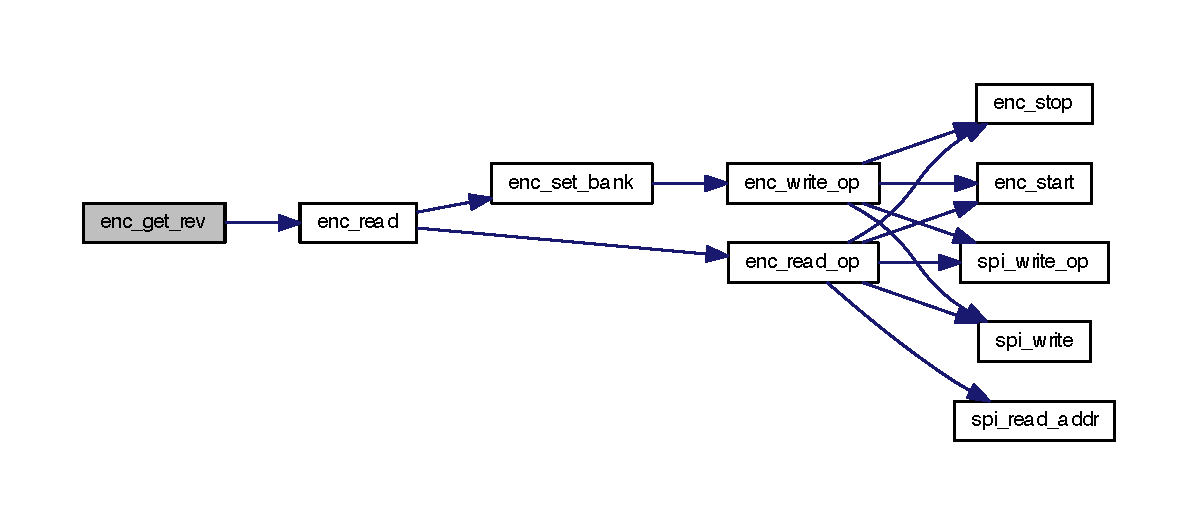
\includegraphics[width=350pt]{enc28j60_8h_a7ac8a98005477e34c31c67395851fc80_cgraph}
\end{center}
\end{figure}


\hypertarget{enc28j60_8h_a9c0a8d055c8531d4ca1aa8e691acf70a}{\index{enc28j60.\+h@{enc28j60.\+h}!enc\+\_\+init@{enc\+\_\+init}}
\index{enc\+\_\+init@{enc\+\_\+init}!enc28j60.\+h@{enc28j60.\+h}}
\subsubsection[{enc\+\_\+init}]{\setlength{\rightskip}{0pt plus 5cm}void enc\+\_\+init (
\begin{DoxyParamCaption}
\item[{uint8\+\_\+t $\ast$}]{}
\end{DoxyParamCaption}
)}}\label{enc28j60_8h_a9c0a8d055c8531d4ca1aa8e691acf70a}


Referenced by main().

\hypertarget{enc28j60_8h_aa75a4325284e67324bcee6b18f882b54}{\index{enc28j60.\+h@{enc28j60.\+h}!enc\+\_\+init\+\_\+phy@{enc\+\_\+init\+\_\+phy}}
\index{enc\+\_\+init\+\_\+phy@{enc\+\_\+init\+\_\+phy}!enc28j60.\+h@{enc28j60.\+h}}
\subsubsection[{enc\+\_\+init\+\_\+phy}]{\setlength{\rightskip}{0pt plus 5cm}void enc\+\_\+init\+\_\+phy (
\begin{DoxyParamCaption}
\item[{void}]{}
\end{DoxyParamCaption}
)}}\label{enc28j60_8h_aa75a4325284e67324bcee6b18f882b54}


initialize the physical interface of E\+N\+C28\+J60 



Definition at line 270 of file enc28j60.\+c.



References enc\+\_\+write\+\_\+phy(), and P\+H\+L\+C\+O\+N.



Referenced by main().



Here is the call graph for this function\+:
\nopagebreak
\begin{figure}[H]
\begin{center}
\leavevmode
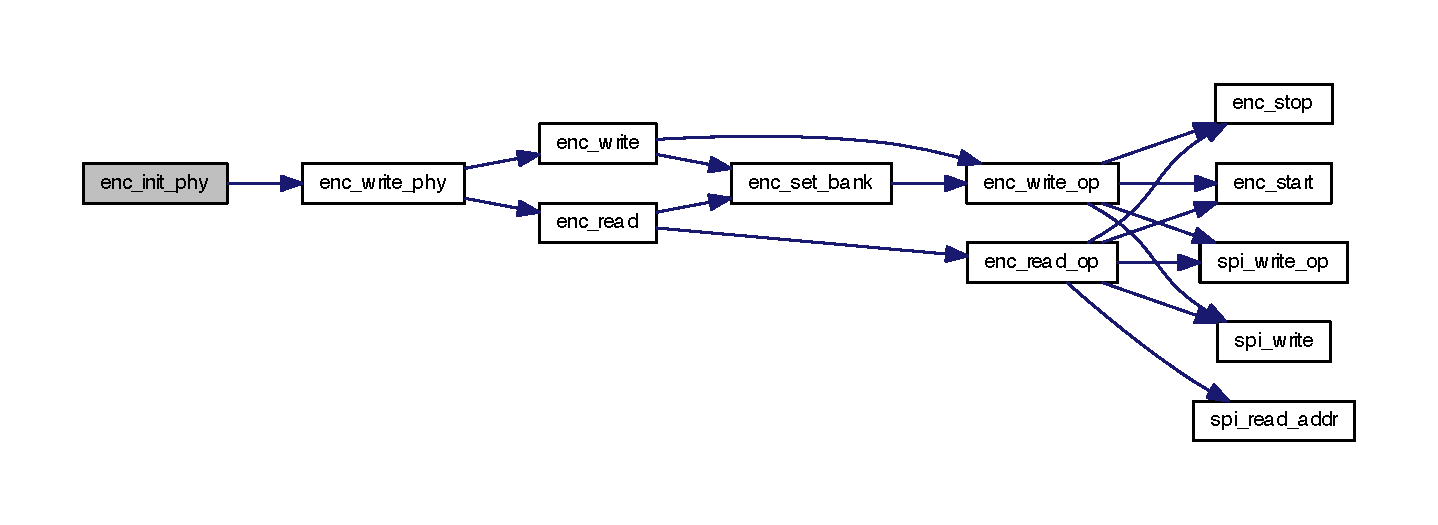
\includegraphics[width=350pt]{enc28j60_8h_aa75a4325284e67324bcee6b18f882b54_cgraph}
\end{center}
\end{figure}


\hypertarget{enc28j60_8h_a42714a50e71f68faacb88f6d09f30e73}{\index{enc28j60.\+h@{enc28j60.\+h}!enc\+\_\+read@{enc\+\_\+read}}
\index{enc\+\_\+read@{enc\+\_\+read}!enc28j60.\+h@{enc28j60.\+h}}
\subsubsection[{enc\+\_\+read}]{\setlength{\rightskip}{0pt plus 5cm}uint8\+\_\+t enc\+\_\+read (
\begin{DoxyParamCaption}
\item[{uint8\+\_\+t}]{addr}
\end{DoxyParamCaption}
)}}\label{enc28j60_8h_a42714a50e71f68faacb88f6d09f30e73}


read from from address of E\+N\+C28\+J60 


\begin{DoxyParams}{Parameters}
{\em addr} & address\\
\hline
\end{DoxyParams}
\begin{DoxyReturn}{Returns}
operation 
\end{DoxyReturn}


Definition at line 235 of file enc28j60.\+c.



References enc\+\_\+read\+\_\+op(), enc\+\_\+set\+\_\+bank(), and R\+E\+A\+D\+\_\+\+C\+T\+R\+L\+\_\+\+R\+E\+G.



Referenced by enc\+\_\+get\+\_\+rev(), enc\+\_\+init(), enc\+\_\+read\+\_\+phy(), enc\+\_\+recv\+\_\+packet(), and enc\+\_\+write\+\_\+phy().



Here is the call graph for this function\+:
\nopagebreak
\begin{figure}[H]
\begin{center}
\leavevmode
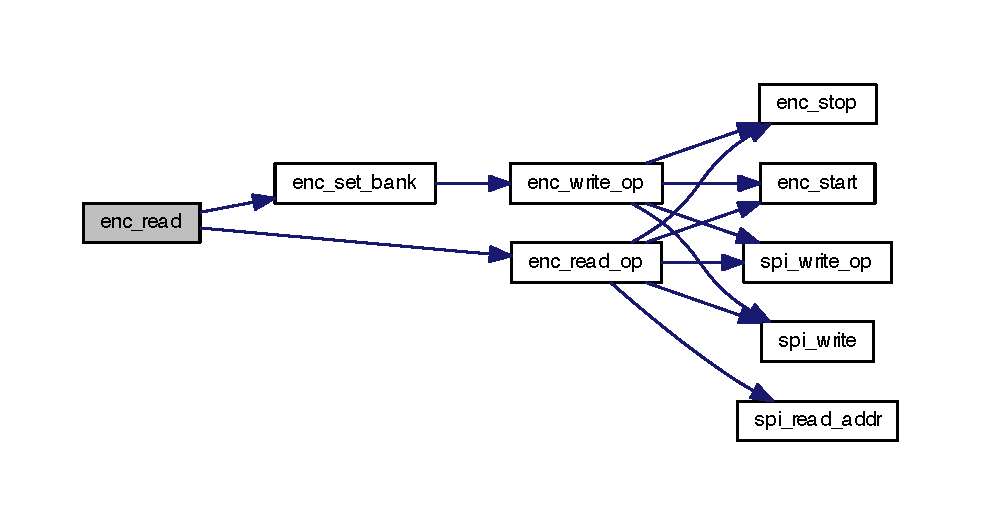
\includegraphics[width=350pt]{enc28j60_8h_a42714a50e71f68faacb88f6d09f30e73_cgraph}
\end{center}
\end{figure}


\hypertarget{enc28j60_8h_a64c815aeeeac3323b0fe272d90a5c0f0}{\index{enc28j60.\+h@{enc28j60.\+h}!enc\+\_\+read\+\_\+buf@{enc\+\_\+read\+\_\+buf}}
\index{enc\+\_\+read\+\_\+buf@{enc\+\_\+read\+\_\+buf}!enc28j60.\+h@{enc28j60.\+h}}
\subsubsection[{enc\+\_\+read\+\_\+buf}]{\setlength{\rightskip}{0pt plus 5cm}void enc\+\_\+read\+\_\+buf (
\begin{DoxyParamCaption}
\item[{uint16\+\_\+t}]{len, }
\item[{uint8\+\_\+t $\ast$}]{data}
\end{DoxyParamCaption}
)}}\label{enc28j60_8h_a64c815aeeeac3323b0fe272d90a5c0f0}


read from the buffer 


\begin{DoxyParams}{Parameters}
{\em len} & length of data \\
\hline
{\em data} & data to read \\
\hline
\end{DoxyParams}


Definition at line 295 of file enc28j60.\+c.



References enc\+\_\+start(), enc\+\_\+stop(), R\+E\+A\+D\+\_\+\+B\+U\+F\+\_\+\+M\+E\+M, spi\+\_\+read(), and spi\+\_\+write().



Referenced by enc\+\_\+recv\+\_\+packet().



Here is the call graph for this function\+:
\nopagebreak
\begin{figure}[H]
\begin{center}
\leavevmode
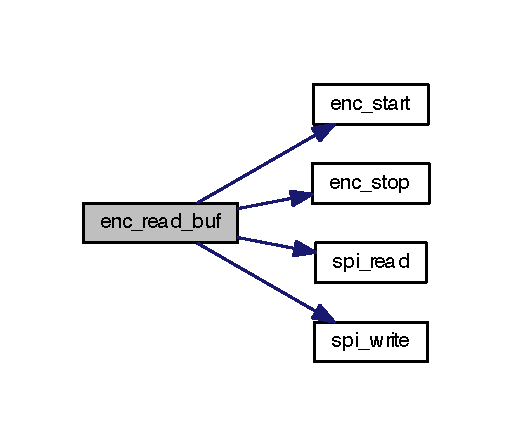
\includegraphics[width=246pt]{enc28j60_8h_a64c815aeeeac3323b0fe272d90a5c0f0_cgraph}
\end{center}
\end{figure}


\hypertarget{enc28j60_8h_aaa5de360d4e46ac044b911c01769f0c4}{\index{enc28j60.\+h@{enc28j60.\+h}!enc\+\_\+read\+\_\+op@{enc\+\_\+read\+\_\+op}}
\index{enc\+\_\+read\+\_\+op@{enc\+\_\+read\+\_\+op}!enc28j60.\+h@{enc28j60.\+h}}
\subsubsection[{enc\+\_\+read\+\_\+op}]{\setlength{\rightskip}{0pt plus 5cm}uint8\+\_\+t enc\+\_\+read\+\_\+op (
\begin{DoxyParamCaption}
\item[{uint8\+\_\+t}]{op, }
\item[{uint8\+\_\+t}]{addr}
\end{DoxyParamCaption}
)}}\label{enc28j60_8h_aaa5de360d4e46ac044b911c01769f0c4}


read the operation from address of E\+N\+C28\+J60 


\begin{DoxyParams}{Parameters}
{\em op} & operation \\
\hline
{\em addr} & address\\
\hline
\end{DoxyParams}
\begin{DoxyReturn}{Returns}
data from S\+P\+I 
\end{DoxyReturn}


Definition at line 251 of file enc28j60.\+c.



References enc\+\_\+start(), enc\+\_\+stop(), spi\+\_\+read\+\_\+addr(), spi\+\_\+write(), and spi\+\_\+write\+\_\+op().



Referenced by enc\+\_\+read(), and enc\+\_\+recv\+\_\+packet().



Here is the call graph for this function\+:
\nopagebreak
\begin{figure}[H]
\begin{center}
\leavevmode
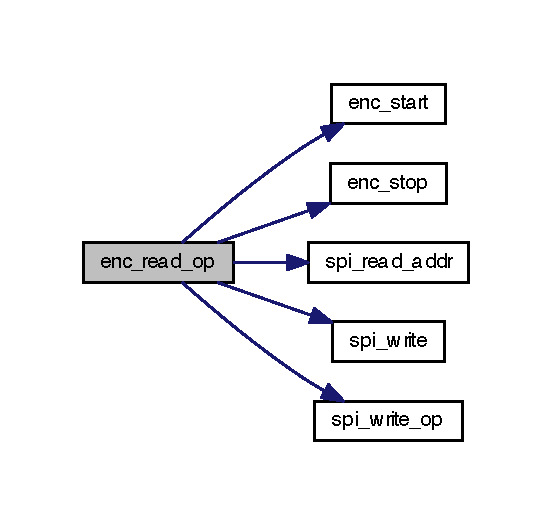
\includegraphics[width=265pt]{enc28j60_8h_aaa5de360d4e46ac044b911c01769f0c4_cgraph}
\end{center}
\end{figure}


\hypertarget{enc28j60_8h_aacaf641612f593cef8136d1fdf8d7bee}{\index{enc28j60.\+h@{enc28j60.\+h}!enc\+\_\+read\+\_\+phy@{enc\+\_\+read\+\_\+phy}}
\index{enc\+\_\+read\+\_\+phy@{enc\+\_\+read\+\_\+phy}!enc28j60.\+h@{enc28j60.\+h}}
\subsubsection[{enc\+\_\+read\+\_\+phy}]{\setlength{\rightskip}{0pt plus 5cm}uint16\+\_\+t enc\+\_\+read\+\_\+phy (
\begin{DoxyParamCaption}
\item[{uint8\+\_\+t}]{addr}
\end{DoxyParamCaption}
)}}\label{enc28j60_8h_aacaf641612f593cef8136d1fdf8d7bee}


read from physical address of E\+N\+C28\+J60 


\begin{DoxyParams}{Parameters}
{\em addr} & address\\
\hline
\end{DoxyParams}
\begin{DoxyReturn}{Returns}
data 
\end{DoxyReturn}


Definition at line 209 of file enc28j60.\+c.



References B\+U\+S\+Y, enc\+\_\+read(), enc\+\_\+write(), M\+I\+C\+M\+D, M\+I\+I\+R\+D, M\+I\+R\+D\+H, M\+I\+R\+D\+L, M\+I\+R\+E\+G\+A\+D\+R, and M\+I\+S\+T\+A\+T.



Here is the call graph for this function\+:
\nopagebreak
\begin{figure}[H]
\begin{center}
\leavevmode
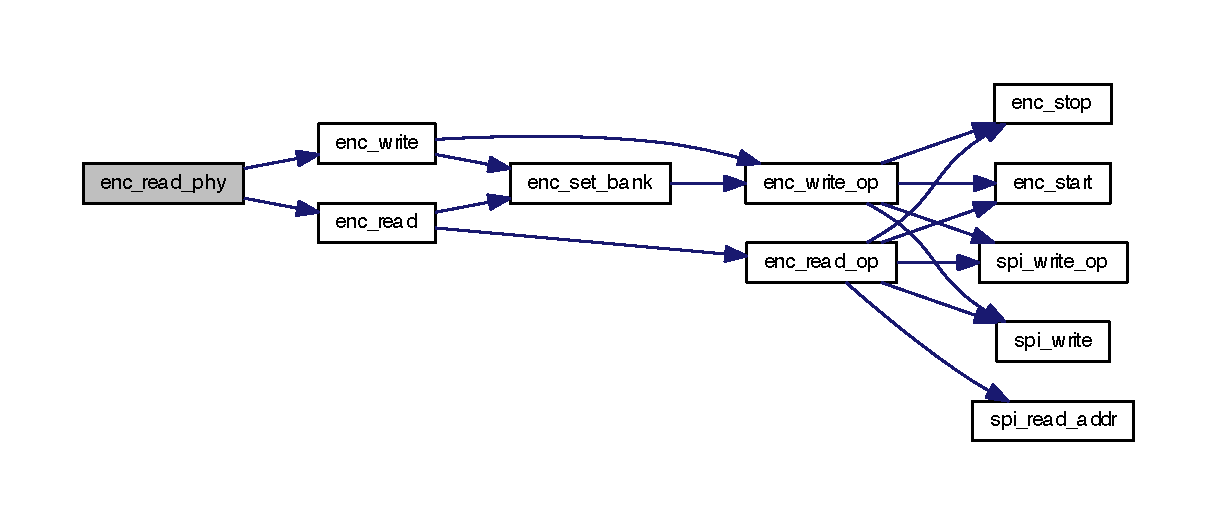
\includegraphics[width=350pt]{enc28j60_8h_aacaf641612f593cef8136d1fdf8d7bee_cgraph}
\end{center}
\end{figure}


\hypertarget{enc28j60_8h_a955683da076de3f92da57d7d06951ae7}{\index{enc28j60.\+h@{enc28j60.\+h}!enc\+\_\+recv\+\_\+packet@{enc\+\_\+recv\+\_\+packet}}
\index{enc\+\_\+recv\+\_\+packet@{enc\+\_\+recv\+\_\+packet}!enc28j60.\+h@{enc28j60.\+h}}
\subsubsection[{enc\+\_\+recv\+\_\+packet}]{\setlength{\rightskip}{0pt plus 5cm}uint16\+\_\+t enc\+\_\+recv\+\_\+packet (
\begin{DoxyParamCaption}
\item[{uint16\+\_\+t}]{maxlen, }
\item[{uint8\+\_\+t $\ast$}]{packet}
\end{DoxyParamCaption}
)}}\label{enc28j60_8h_a955683da076de3f92da57d7d06951ae7}


receive a packet from ethernet 


\begin{DoxyParams}{Parameters}
{\em maxlen} & maximum length of packet to receive \\
\hline
{\em packet} & packet to receive\\
\hline
\end{DoxyParams}
\begin{DoxyReturn}{Returns}
length of received packet 
\end{DoxyReturn}


Definition at line 368 of file enc28j60.\+c.



References B\+I\+T\+\_\+\+F\+I\+E\+L\+D\+\_\+\+S\+E\+T, E\+C\+O\+N2, enc\+\_\+read(), enc\+\_\+read\+\_\+buf(), enc\+\_\+read\+\_\+op(), enc\+\_\+write(), enc\+\_\+write\+\_\+op(), E\+P\+K\+T\+C\+N\+T, E\+R\+D\+P\+T\+H, E\+R\+D\+P\+T\+L, E\+R\+X\+R\+D\+P\+T\+H, E\+R\+X\+R\+D\+P\+T\+L, M\+I\+N, p\+\_\+next, P\+K\+T\+D\+E\+C, and R\+E\+A\+D\+\_\+\+B\+U\+F\+\_\+\+M\+E\+M.



Referenced by main().



Here is the call graph for this function\+:
\nopagebreak
\begin{figure}[H]
\begin{center}
\leavevmode
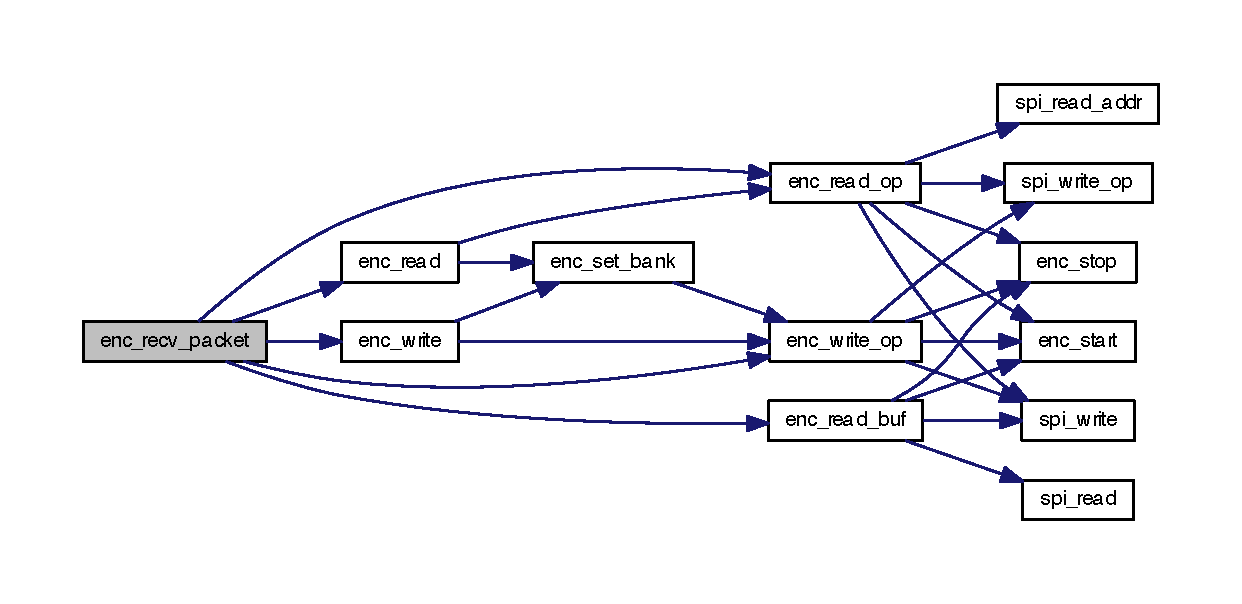
\includegraphics[width=350pt]{enc28j60_8h_a955683da076de3f92da57d7d06951ae7_cgraph}
\end{center}
\end{figure}


\hypertarget{enc28j60_8h_abcc7d56a9babb64610bd346cdaef81a6}{\index{enc28j60.\+h@{enc28j60.\+h}!enc\+\_\+send\+\_\+packet@{enc\+\_\+send\+\_\+packet}}
\index{enc\+\_\+send\+\_\+packet@{enc\+\_\+send\+\_\+packet}!enc28j60.\+h@{enc28j60.\+h}}
\subsubsection[{enc\+\_\+send\+\_\+packet}]{\setlength{\rightskip}{0pt plus 5cm}void enc\+\_\+send\+\_\+packet (
\begin{DoxyParamCaption}
\item[{uint16\+\_\+t}]{len, }
\item[{uint8\+\_\+t $\ast$}]{packet}
\end{DoxyParamCaption}
)}}\label{enc28j60_8h_abcc7d56a9babb64610bd346cdaef81a6}


send a packet to ethernet 


\begin{DoxyParams}{Parameters}
{\em len} & length of packet \\
\hline
{\em packet} & packet to send \\
\hline
\end{DoxyParams}


Definition at line 344 of file enc28j60.\+c.



References B\+I\+T\+\_\+\+F\+I\+E\+L\+D\+\_\+\+S\+E\+T, E\+C\+O\+N1, enc\+\_\+write(), enc\+\_\+write\+\_\+buf(), enc\+\_\+write\+\_\+op(), E\+T\+X\+N\+D\+H, E\+T\+X\+N\+D\+L, E\+W\+R\+P\+T\+H, E\+W\+R\+P\+T\+L, T\+X\+\_\+\+S\+T\+A\+R\+T\+\_\+\+I\+N\+I\+T, T\+X\+R\+T\+S, and W\+R\+I\+T\+E\+\_\+\+B\+U\+F\+\_\+\+M\+E\+M.



Referenced by arp\+\_\+answer(), echo\+\_\+reply(), and udp\+\_\+reply().



Here is the call graph for this function\+:
\nopagebreak
\begin{figure}[H]
\begin{center}
\leavevmode
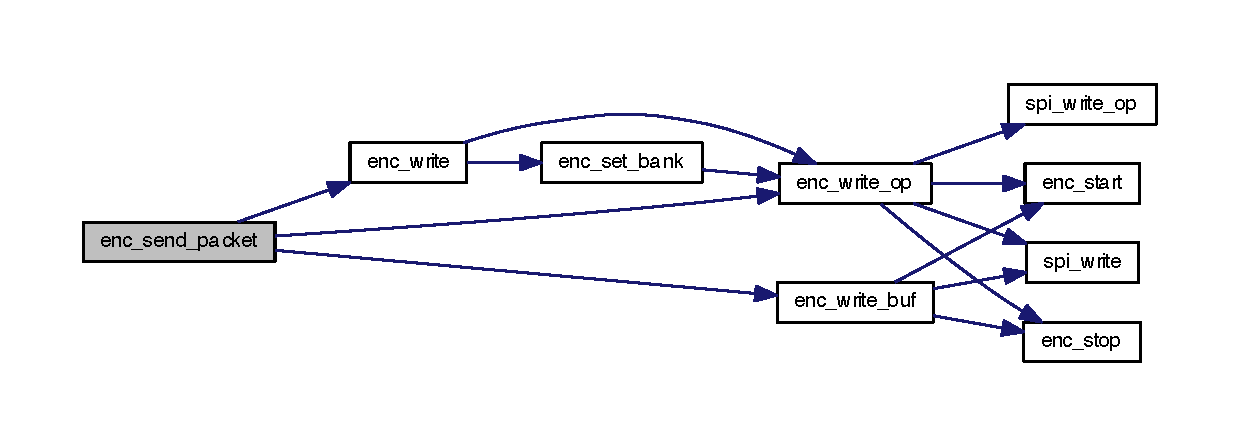
\includegraphics[width=350pt]{enc28j60_8h_abcc7d56a9babb64610bd346cdaef81a6_cgraph}
\end{center}
\end{figure}


\hypertarget{enc28j60_8h_ac9481db892dd46048540a834032f8ef7}{\index{enc28j60.\+h@{enc28j60.\+h}!enc\+\_\+set\+\_\+bank@{enc\+\_\+set\+\_\+bank}}
\index{enc\+\_\+set\+\_\+bank@{enc\+\_\+set\+\_\+bank}!enc28j60.\+h@{enc28j60.\+h}}
\subsubsection[{enc\+\_\+set\+\_\+bank}]{\setlength{\rightskip}{0pt plus 5cm}void enc\+\_\+set\+\_\+bank (
\begin{DoxyParamCaption}
\item[{uint8\+\_\+t}]{addr}
\end{DoxyParamCaption}
)}}\label{enc28j60_8h_ac9481db892dd46048540a834032f8ef7}


set the bank on address 


\begin{DoxyParams}{Parameters}
{\em addr} & address to set \\
\hline
\end{DoxyParams}


Definition at line 174 of file enc28j60.\+c.



References A\+D\+D\+R\+\_\+\+M\+A\+S\+K, B\+A\+N\+K\+\_\+\+M\+A\+S\+K, B\+I\+T\+\_\+\+F\+I\+E\+L\+D\+\_\+\+C\+L\+R, B\+I\+T\+\_\+\+F\+I\+E\+L\+D\+\_\+\+S\+E\+T, B\+S\+E\+L0, B\+S\+E\+L1, E\+C\+O\+N1, enc\+\_\+bank, and enc\+\_\+write\+\_\+op().



Referenced by enc\+\_\+init(), enc\+\_\+read(), and enc\+\_\+write().



Here is the call graph for this function\+:
\nopagebreak
\begin{figure}[H]
\begin{center}
\leavevmode
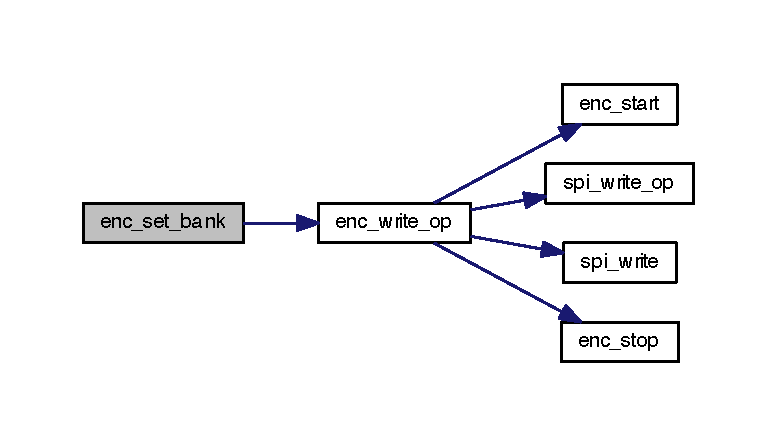
\includegraphics[width=350pt]{enc28j60_8h_ac9481db892dd46048540a834032f8ef7_cgraph}
\end{center}
\end{figure}


\hypertarget{enc28j60_8h_aa518d6801d39ef8d7ad828b0f35684f0}{\index{enc28j60.\+h@{enc28j60.\+h}!enc\+\_\+set\+\_\+mac@{enc\+\_\+set\+\_\+mac}}
\index{enc\+\_\+set\+\_\+mac@{enc\+\_\+set\+\_\+mac}!enc28j60.\+h@{enc28j60.\+h}}
\subsubsection[{enc\+\_\+set\+\_\+mac}]{\setlength{\rightskip}{0pt plus 5cm}void enc\+\_\+set\+\_\+mac (
\begin{DoxyParamCaption}
\item[{uint8\+\_\+t $\ast$}]{}
\end{DoxyParamCaption}
)}}\label{enc28j60_8h_aa518d6801d39ef8d7ad828b0f35684f0}
\hypertarget{enc28j60_8h_a6ae6915ab4363819a3492bd8509263e5}{\index{enc28j60.\+h@{enc28j60.\+h}!enc\+\_\+start@{enc\+\_\+start}}
\index{enc\+\_\+start@{enc\+\_\+start}!enc28j60.\+h@{enc28j60.\+h}}
\subsubsection[{enc\+\_\+start}]{\setlength{\rightskip}{0pt plus 5cm}void enc\+\_\+start (
\begin{DoxyParamCaption}
\item[{void}]{}
\end{DoxyParamCaption}
)}}\label{enc28j60_8h_a6ae6915ab4363819a3492bd8509263e5}


start E\+N\+C28\+J60 pin to write or to read 



Definition at line 38 of file enc28j60.\+c.



References E\+N\+C\+\_\+\+C\+T\+R\+L\+\_\+\+C\+S, and E\+N\+C\+\_\+\+C\+T\+R\+L\+\_\+\+P\+O\+R\+T.



Referenced by enc\+\_\+read\+\_\+buf(), enc\+\_\+read\+\_\+op(), enc\+\_\+write\+\_\+buf(), and enc\+\_\+write\+\_\+op().

\hypertarget{enc28j60_8h_a63e6002e7cdb7ac2433fcb6fb4fc0b16}{\index{enc28j60.\+h@{enc28j60.\+h}!enc\+\_\+stop@{enc\+\_\+stop}}
\index{enc\+\_\+stop@{enc\+\_\+stop}!enc28j60.\+h@{enc28j60.\+h}}
\subsubsection[{enc\+\_\+stop}]{\setlength{\rightskip}{0pt plus 5cm}void enc\+\_\+stop (
\begin{DoxyParamCaption}
\item[{void}]{}
\end{DoxyParamCaption}
)}}\label{enc28j60_8h_a63e6002e7cdb7ac2433fcb6fb4fc0b16}


stop the E\+N\+C28\+J60 pin 



Definition at line 47 of file enc28j60.\+c.



References E\+N\+C\+\_\+\+C\+T\+R\+L\+\_\+\+C\+S, and E\+N\+C\+\_\+\+C\+T\+R\+L\+\_\+\+P\+O\+R\+T.



Referenced by enc\+\_\+read\+\_\+buf(), enc\+\_\+read\+\_\+op(), enc\+\_\+write\+\_\+buf(), and enc\+\_\+write\+\_\+op().

\hypertarget{enc28j60_8h_a9baf5880395c0b49cd2cfccf3dc690e2}{\index{enc28j60.\+h@{enc28j60.\+h}!enc\+\_\+write@{enc\+\_\+write}}
\index{enc\+\_\+write@{enc\+\_\+write}!enc28j60.\+h@{enc28j60.\+h}}
\subsubsection[{enc\+\_\+write}]{\setlength{\rightskip}{0pt plus 5cm}void enc\+\_\+write (
\begin{DoxyParamCaption}
\item[{uint8\+\_\+t}]{addr, }
\item[{uint8\+\_\+t}]{data}
\end{DoxyParamCaption}
)}}\label{enc28j60_8h_a9baf5880395c0b49cd2cfccf3dc690e2}


write on E\+N\+C28\+J60 


\begin{DoxyParams}{Parameters}
{\em addr} & address to write \\
\hline
{\em data} & data to send \\
\hline
\end{DoxyParams}


Definition at line 162 of file enc28j60.\+c.



References enc\+\_\+set\+\_\+bank(), enc\+\_\+write\+\_\+op(), and W\+R\+I\+T\+E\+\_\+\+C\+T\+R\+L\+\_\+\+R\+E\+G.



Referenced by enc\+\_\+init(), enc\+\_\+read\+\_\+phy(), enc\+\_\+recv\+\_\+packet(), enc\+\_\+send\+\_\+packet(), enc\+\_\+set\+\_\+mac(), and enc\+\_\+write\+\_\+phy().



Here is the call graph for this function\+:
\nopagebreak
\begin{figure}[H]
\begin{center}
\leavevmode
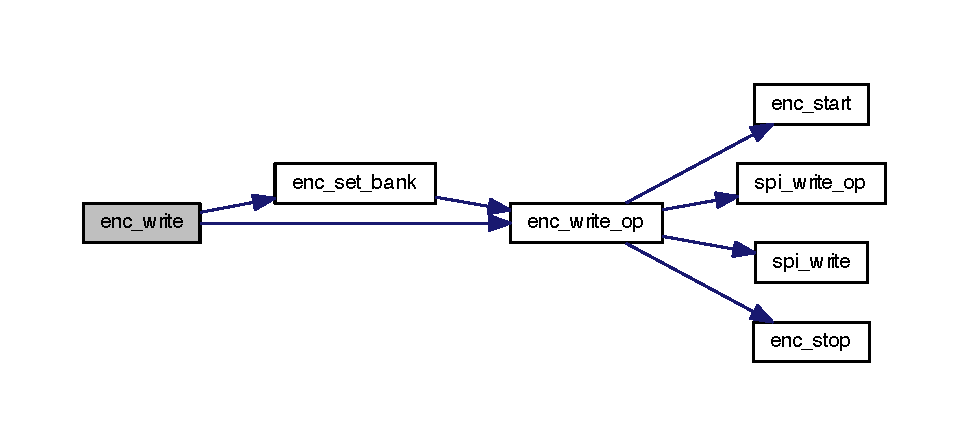
\includegraphics[width=350pt]{enc28j60_8h_a9baf5880395c0b49cd2cfccf3dc690e2_cgraph}
\end{center}
\end{figure}


\hypertarget{enc28j60_8h_a22151e93b50167d60ea05a0806bed7d0}{\index{enc28j60.\+h@{enc28j60.\+h}!enc\+\_\+write\+\_\+buf@{enc\+\_\+write\+\_\+buf}}
\index{enc\+\_\+write\+\_\+buf@{enc\+\_\+write\+\_\+buf}!enc28j60.\+h@{enc28j60.\+h}}
\subsubsection[{enc\+\_\+write\+\_\+buf}]{\setlength{\rightskip}{0pt plus 5cm}void enc\+\_\+write\+\_\+buf (
\begin{DoxyParamCaption}
\item[{uint16\+\_\+t}]{len, }
\item[{uint8\+\_\+t $\ast$}]{data}
\end{DoxyParamCaption}
)}}\label{enc28j60_8h_a22151e93b50167d60ea05a0806bed7d0}


write the buffer 


\begin{DoxyParams}{Parameters}
{\em len} & length of data \\
\hline
{\em data} & data \\
\hline
\end{DoxyParams}


Definition at line 314 of file enc28j60.\+c.



References enc\+\_\+start(), enc\+\_\+stop(), spi\+\_\+write(), and W\+R\+I\+T\+E\+\_\+\+B\+U\+F\+\_\+\+M\+E\+M.



Referenced by enc\+\_\+send\+\_\+packet().



Here is the call graph for this function\+:
\nopagebreak
\begin{figure}[H]
\begin{center}
\leavevmode
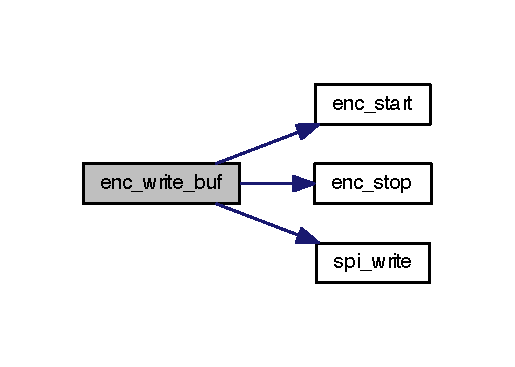
\includegraphics[width=247pt]{enc28j60_8h_a22151e93b50167d60ea05a0806bed7d0_cgraph}
\end{center}
\end{figure}


\hypertarget{enc28j60_8h_a7b7b73cf7da394dcfd8425e69eb866c5}{\index{enc28j60.\+h@{enc28j60.\+h}!enc\+\_\+write\+\_\+op@{enc\+\_\+write\+\_\+op}}
\index{enc\+\_\+write\+\_\+op@{enc\+\_\+write\+\_\+op}!enc28j60.\+h@{enc28j60.\+h}}
\subsubsection[{enc\+\_\+write\+\_\+op}]{\setlength{\rightskip}{0pt plus 5cm}void enc\+\_\+write\+\_\+op (
\begin{DoxyParamCaption}
\item[{uint8\+\_\+t}]{op, }
\item[{uint8\+\_\+t}]{addr, }
\item[{uint8\+\_\+t}]{data}
\end{DoxyParamCaption}
)}}\label{enc28j60_8h_a7b7b73cf7da394dcfd8425e69eb866c5}


write the operation 


\begin{DoxyParams}{Parameters}
{\em op} & operation to write on S\+P\+I \\
\hline
{\em addr} & address to write \\
\hline
{\em data} & data to send on S\+P\+I \\
\hline
\end{DoxyParams}


Definition at line 145 of file enc28j60.\+c.



References enc\+\_\+start(), enc\+\_\+stop(), spi\+\_\+write(), and spi\+\_\+write\+\_\+op().



Referenced by enc\+\_\+init(), enc\+\_\+recv\+\_\+packet(), enc\+\_\+send\+\_\+packet(), enc\+\_\+set\+\_\+bank(), and enc\+\_\+write().



Here is the call graph for this function\+:
\nopagebreak
\begin{figure}[H]
\begin{center}
\leavevmode
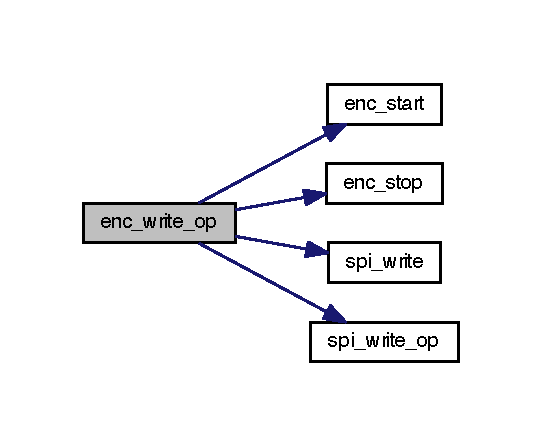
\includegraphics[width=260pt]{enc28j60_8h_a7b7b73cf7da394dcfd8425e69eb866c5_cgraph}
\end{center}
\end{figure}


\hypertarget{enc28j60_8h_ab2e6a8f9117e6c212139571a96f0e001}{\index{enc28j60.\+h@{enc28j60.\+h}!enc\+\_\+write\+\_\+phy@{enc\+\_\+write\+\_\+phy}}
\index{enc\+\_\+write\+\_\+phy@{enc\+\_\+write\+\_\+phy}!enc28j60.\+h@{enc28j60.\+h}}
\subsubsection[{enc\+\_\+write\+\_\+phy}]{\setlength{\rightskip}{0pt plus 5cm}void enc\+\_\+write\+\_\+phy (
\begin{DoxyParamCaption}
\item[{uint8\+\_\+t}]{addr, }
\item[{uint16\+\_\+t}]{data}
\end{DoxyParamCaption}
)}}\label{enc28j60_8h_ab2e6a8f9117e6c212139571a96f0e001}


write the data on E\+N\+C28\+J60 physical address 


\begin{DoxyParams}{Parameters}
{\em addr} & address \\
\hline
{\em data} & data \\
\hline
\end{DoxyParams}


Definition at line 190 of file enc28j60.\+c.



References B\+U\+S\+Y, enc\+\_\+read(), enc\+\_\+write(), M\+I\+R\+E\+G\+A\+D\+R, M\+I\+S\+T\+A\+T, M\+I\+W\+R\+H, and M\+I\+W\+R\+L.



Referenced by enc\+\_\+init(), and enc\+\_\+init\+\_\+phy().



Here is the call graph for this function\+:
\nopagebreak
\begin{figure}[H]
\begin{center}
\leavevmode
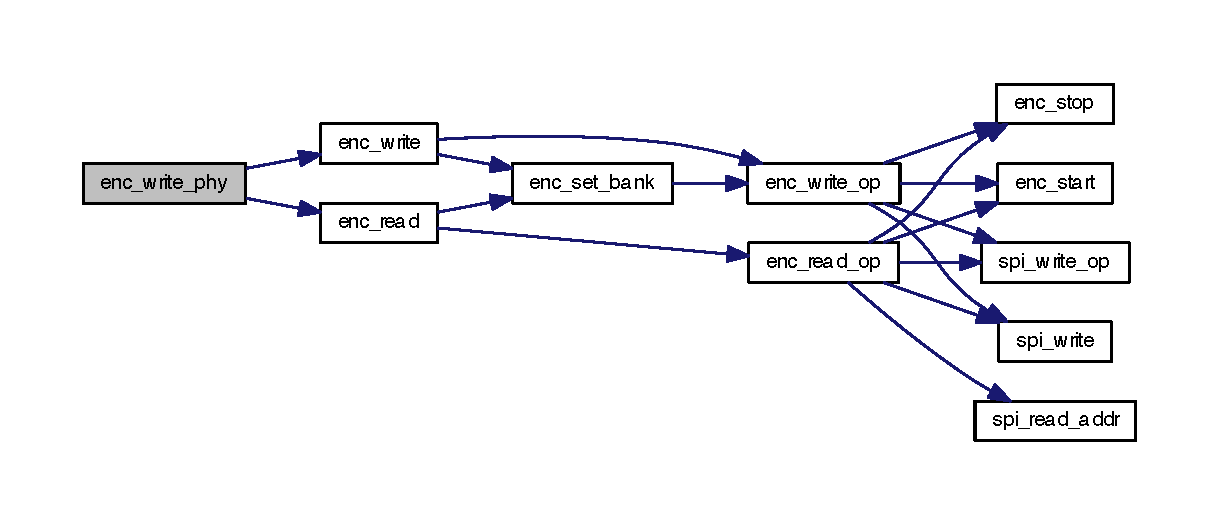
\includegraphics[width=350pt]{enc28j60_8h_ab2e6a8f9117e6c212139571a96f0e001_cgraph}
\end{center}
\end{figure}



\hypertarget{enc28j60_8c}{\section{driver/enc28j60.c File Reference}
\label{enc28j60_8c}\index{driver/enc28j60.\+c@{driver/enc28j60.\+c}}
}


E\+N\+C28\+J60 ethernet driver.  


{\ttfamily \#include $<$board/freq.\+h$>$}\\*
{\ttfamily \#include $<$device/enc28j60.\+h$>$}\\*
{\ttfamily \#include $<$driver/spi.\+h$>$}\\*
Include dependency graph for enc28j60.\+c\+:
\nopagebreak
\begin{figure}[H]
\begin{center}
\leavevmode
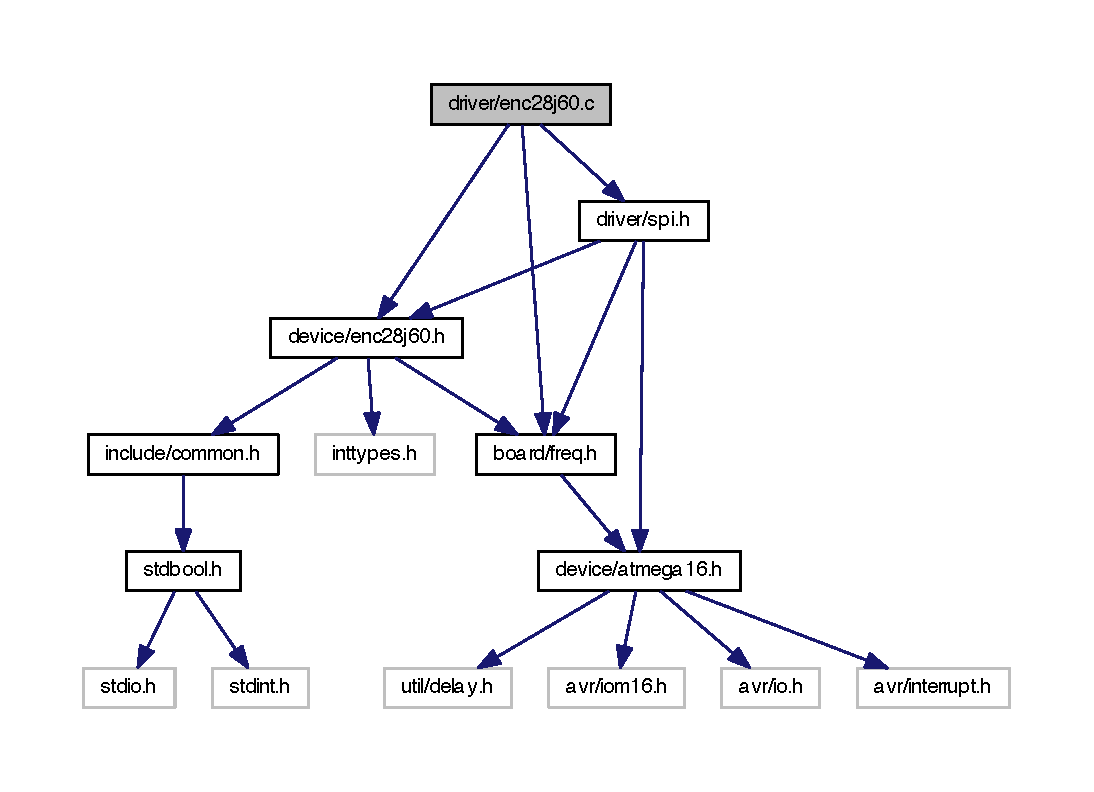
\includegraphics[width=350pt]{enc28j60_8c__incl}
\end{center}
\end{figure}
\subsection*{Functions}
\begin{DoxyCompactItemize}
\item 
void \hyperlink{enc28j60_8c_a6ae6915ab4363819a3492bd8509263e5}{enc\+\_\+start} (void)
\begin{DoxyCompactList}\small\item\em start E\+N\+C28\+J60 pin to write or to read \end{DoxyCompactList}\item 
void \hyperlink{enc28j60_8c_a63e6002e7cdb7ac2433fcb6fb4fc0b16}{enc\+\_\+stop} (void)
\begin{DoxyCompactList}\small\item\em stop the E\+N\+C28\+J60 pin \end{DoxyCompactList}\item 
void \hyperlink{enc28j60_8c_a3de012f2c3b25ad182f94f5b1ab9a771}{enc\+\_\+set\+\_\+mac} (uint8\+\_\+t \hyperlink{main_8c_ae0177d7710b28f95720d54e2b1d37d65}{mymac}\mbox{[}$\,$\mbox{]})
\begin{DoxyCompactList}\small\item\em set the mac-\/address to B\+A\+N\+K3 register \end{DoxyCompactList}\item 
void \hyperlink{enc28j60_8c_a786c5765ce9469049ee56d2ca66dcf25}{enc\+\_\+init} (uint8\+\_\+t \hyperlink{main_8c_ae0177d7710b28f95720d54e2b1d37d65}{mymac}\mbox{[}$\,$\mbox{]})
\begin{DoxyCompactList}\small\item\em initialize the E\+N\+C28\+J60 \end{DoxyCompactList}\item 
void \hyperlink{enc28j60_8c_ab64d8270b5a710a2ff635d4449c91a08}{enc\+\_\+write\+\_\+op} (uint8\+\_\+t op, uint8\+\_\+t addr, uint8\+\_\+t data)
\begin{DoxyCompactList}\small\item\em write the operation \end{DoxyCompactList}\item 
void \hyperlink{enc28j60_8c_a7520f33b52393de8d0e3caa796e0baa2}{enc\+\_\+write} (uint8\+\_\+t addr, uint8\+\_\+t data)
\begin{DoxyCompactList}\small\item\em write on E\+N\+C28\+J60 \end{DoxyCompactList}\item 
void \hyperlink{enc28j60_8c_ac175ce9462129e5d35f06935aa42c9f6}{enc\+\_\+set\+\_\+bank} (uint8\+\_\+t addr)
\begin{DoxyCompactList}\small\item\em set the bank on address \end{DoxyCompactList}\item 
void \hyperlink{enc28j60_8c_ab6908af0f98d4b54d35cbcd699119346}{enc\+\_\+write\+\_\+phy} (uint8\+\_\+t addr, uint16\+\_\+t data)
\begin{DoxyCompactList}\small\item\em write the data on E\+N\+C28\+J60 physical address \end{DoxyCompactList}\item 
uint16\+\_\+t \hyperlink{enc28j60_8c_ab1b8f7c1f5dbcb0e500da8ed87219cd7}{enc\+\_\+read\+\_\+phy} (uint8\+\_\+t addr)
\begin{DoxyCompactList}\small\item\em read from physical address of E\+N\+C28\+J60 \end{DoxyCompactList}\item 
uint8\+\_\+t \hyperlink{enc28j60_8c_a0619a7608315f0484d493da171ee37ae}{enc\+\_\+read} (uint8\+\_\+t addr)
\begin{DoxyCompactList}\small\item\em read from from address of E\+N\+C28\+J60 \end{DoxyCompactList}\item 
uint8\+\_\+t \hyperlink{enc28j60_8c_a28f10fce3f5c8c1e29efcce27932d149}{enc\+\_\+read\+\_\+op} (uint8\+\_\+t op, uint8\+\_\+t addr)
\begin{DoxyCompactList}\small\item\em read the operation from address of E\+N\+C28\+J60 \end{DoxyCompactList}\item 
void \hyperlink{enc28j60_8c_aa75a4325284e67324bcee6b18f882b54}{enc\+\_\+init\+\_\+phy} (void)
\begin{DoxyCompactList}\small\item\em initialize the physical interface of E\+N\+C28\+J60 \end{DoxyCompactList}\item 
void \hyperlink{enc28j60_8c_ae07e529513d99c8612e7878b7524109d}{enc\+\_\+read\+\_\+buf} (uint16\+\_\+t len, uint8\+\_\+t $\ast$data)
\begin{DoxyCompactList}\small\item\em read from the buffer \end{DoxyCompactList}\item 
void \hyperlink{enc28j60_8c_a8ae17d4efc162d054952cc4cb80d422c}{enc\+\_\+write\+\_\+buf} (uint16\+\_\+t len, uint8\+\_\+t $\ast$data)
\begin{DoxyCompactList}\small\item\em write the buffer \end{DoxyCompactList}\item 
uint8\+\_\+t \hyperlink{enc28j60_8c_a7ac8a98005477e34c31c67395851fc80}{enc\+\_\+get\+\_\+rev} (void)
\begin{DoxyCompactList}\small\item\em get the revision of E\+N\+C28\+J60 \end{DoxyCompactList}\item 
void \hyperlink{enc28j60_8c_a094a800fcadc3033c6d1e90d2eecba23}{enc\+\_\+send\+\_\+packet} (uint16\+\_\+t len, uint8\+\_\+t $\ast$packet)
\begin{DoxyCompactList}\small\item\em send a packet to ethernet \end{DoxyCompactList}\item 
uint16\+\_\+t \hyperlink{enc28j60_8c_a412f11a9dbdb9cf9bf812751044f4d4f}{enc\+\_\+recv\+\_\+packet} (uint16\+\_\+t maxlen, uint8\+\_\+t $\ast$packet)
\begin{DoxyCompactList}\small\item\em receive a packet from ethernet \end{DoxyCompactList}\end{DoxyCompactItemize}
\subsection*{Variables}
\begin{DoxyCompactItemize}
\item 
uint8\+\_\+t \hyperlink{enc28j60_8c_a8cf887c83e16783a97183adf9b0bd5eb}{enc\+\_\+bank}
\item 
unsigned int \hyperlink{enc28j60_8c_ad7e304a214204367dd0528e5df3c59f0}{p\+\_\+next}
\end{DoxyCompactItemize}


\subsection{Detailed Description}
E\+N\+C28\+J60 ethernet driver. 

\begin{DoxyAuthor}{Author}
M. Ozgan, \href{mailto:mozgan@mozgan.org}{\tt mozgan@mozgan.\+org} 
\end{DoxyAuthor}
\begin{DoxyVersion}{Version}
1.\+0 
\end{DoxyVersion}
\begin{DoxyDate}{Date}
19.\+08.\+2013 18\+:51\+:18 
\end{DoxyDate}
\begin{DoxyParagraph}{Compiler}
gcc (on Mac, and 4.\+4\+B\+S\+D) 
\end{DoxyParagraph}
\begin{DoxyParagraph}{Company}
T\+U Wien 
\end{DoxyParagraph}


\begin{DoxyRefDesc}{Bug}
\item[\hyperlink{bug__bug000004}{Bug}]'enc\+\_\+send\+\_\+packet' gives a warning with compiler option '-\/\+Woverflow'. You can devide as bytes the 16-\/bit registers. \end{DoxyRefDesc}
\begin{DoxyRefDesc}{Todo}
\item[\hyperlink{todo__todo000004}{Todo}]none \end{DoxyRefDesc}


Definition in file \hyperlink{enc28j60_8c_source}{enc28j60.\+c}.



\subsection{Function Documentation}
\hypertarget{enc28j60_8c_a7ac8a98005477e34c31c67395851fc80}{\index{enc28j60.\+c@{enc28j60.\+c}!enc\+\_\+get\+\_\+rev@{enc\+\_\+get\+\_\+rev}}
\index{enc\+\_\+get\+\_\+rev@{enc\+\_\+get\+\_\+rev}!enc28j60.\+c@{enc28j60.\+c}}
\subsubsection[{enc\+\_\+get\+\_\+rev}]{\setlength{\rightskip}{0pt plus 5cm}uint8\+\_\+t enc\+\_\+get\+\_\+rev (
\begin{DoxyParamCaption}
\item[{void}]{}
\end{DoxyParamCaption}
)}}\label{enc28j60_8c_a7ac8a98005477e34c31c67395851fc80}


get the revision of E\+N\+C28\+J60 

\begin{DoxyReturn}{Returns}
revision 
\end{DoxyReturn}


Definition at line 332 of file enc28j60.\+c.



References enc\+\_\+read(), and E\+R\+E\+V\+I\+D.



Here is the call graph for this function\+:
\nopagebreak
\begin{figure}[H]
\begin{center}
\leavevmode
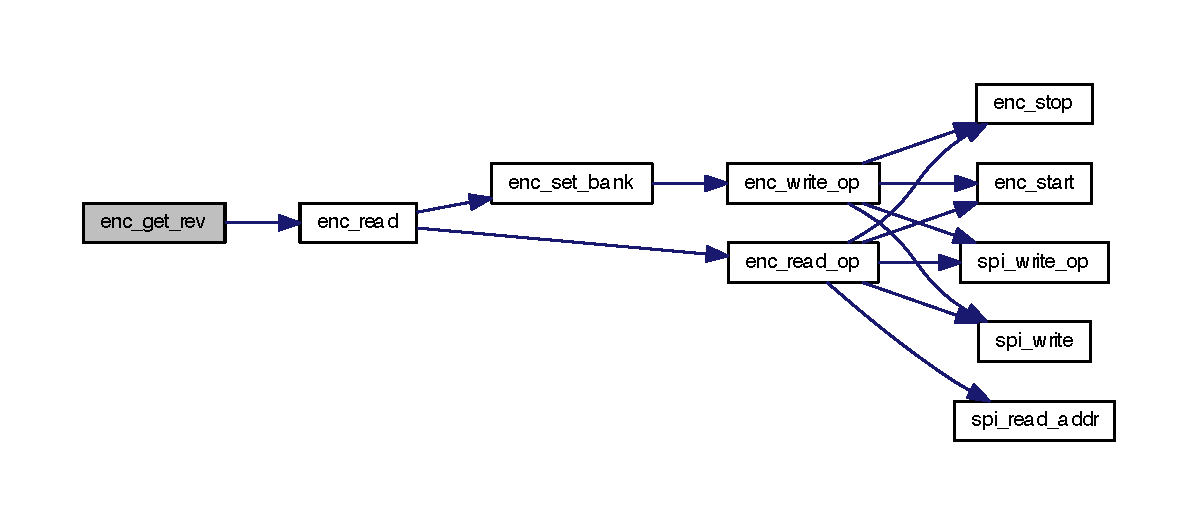
\includegraphics[width=350pt]{enc28j60_8c_a7ac8a98005477e34c31c67395851fc80_cgraph}
\end{center}
\end{figure}


\hypertarget{enc28j60_8c_a786c5765ce9469049ee56d2ca66dcf25}{\index{enc28j60.\+c@{enc28j60.\+c}!enc\+\_\+init@{enc\+\_\+init}}
\index{enc\+\_\+init@{enc\+\_\+init}!enc28j60.\+c@{enc28j60.\+c}}
\subsubsection[{enc\+\_\+init}]{\setlength{\rightskip}{0pt plus 5cm}void enc\+\_\+init (
\begin{DoxyParamCaption}
\item[{uint8\+\_\+t}]{mymac\mbox{[}$\,$\mbox{]}}
\end{DoxyParamCaption}
)}}\label{enc28j60_8c_a786c5765ce9469049ee56d2ca66dcf25}


initialize the E\+N\+C28\+J60 


\begin{DoxyParams}{Parameters}
{\em mymac\mbox{[}$\,$\mbox{]}} & my mac address \\
\hline
\end{DoxyParams}


Definition at line 74 of file enc28j60.\+c.



References B\+I\+T\+\_\+\+F\+I\+E\+L\+D\+\_\+\+S\+E\+T, C\+L\+K\+R\+D\+Y, C\+R\+C\+E\+N, E\+\_\+\+R\+X\+E\+N, E\+C\+O\+N1, E\+I\+E, E\+N\+C\+\_\+\+C\+T\+R\+L\+\_\+\+C\+S, E\+N\+C\+\_\+\+C\+T\+R\+L\+\_\+\+D\+D\+R, E\+N\+C\+\_\+\+C\+T\+R\+L\+\_\+\+P\+O\+R\+T, enc\+\_\+read(), enc\+\_\+set\+\_\+bank(), enc\+\_\+set\+\_\+mac(), enc\+\_\+write(), enc\+\_\+write\+\_\+op(), enc\+\_\+write\+\_\+phy(), E\+P\+M\+C\+S\+H, E\+P\+M\+C\+S\+L, E\+P\+M\+M0, E\+P\+M\+M1, E\+R\+X\+F\+C\+O\+N, E\+R\+X\+N\+D\+H, E\+R\+X\+N\+D\+L, E\+R\+X\+R\+D\+P\+T\+H, E\+R\+X\+R\+D\+P\+T\+L, E\+R\+X\+S\+T\+H, E\+R\+X\+S\+T\+L, E\+S\+T\+A\+T, E\+T\+X\+N\+D\+H, E\+T\+X\+N\+D\+L, E\+T\+X\+S\+T\+H, E\+T\+X\+S\+T\+L, F\+R\+M\+L\+N\+E\+N, H\+D\+L\+D\+I\+S, I\+N\+T\+I\+E, M\+A\+B\+B\+I\+P\+G, M\+A\+C\+O\+N1, M\+A\+C\+O\+N2, M\+A\+C\+O\+N3, M\+A\+I\+P\+G\+H, M\+A\+I\+P\+G\+L, M\+A\+M\+X\+F\+L\+H, M\+A\+M\+X\+F\+L\+L, M\+A\+R\+X\+E\+N, M\+A\+X\+\_\+\+F\+R\+A\+M\+E\+\_\+\+L\+E\+N, p\+\_\+next, P\+A\+D\+C\+F\+G0, P\+H\+C\+O\+N2, P\+K\+T\+I\+E, P\+M\+E\+N, R\+X\+\_\+\+S\+T\+A\+R\+T\+\_\+\+I\+N\+I\+T, R\+X\+\_\+\+S\+T\+O\+P\+\_\+\+I\+N\+I\+T, R\+X\+P\+A\+U\+S, S\+O\+F\+T\+\_\+\+R\+E\+S\+E\+T, spi\+\_\+init(), T\+X\+\_\+\+S\+T\+A\+R\+T\+\_\+\+I\+N\+I\+T, T\+X\+\_\+\+S\+T\+O\+P\+\_\+\+I\+N\+I\+T, T\+X\+C\+R\+C\+E\+N, T\+X\+P\+A\+U\+S, and U\+C\+E\+N.



Here is the call graph for this function\+:
\nopagebreak
\begin{figure}[H]
\begin{center}
\leavevmode
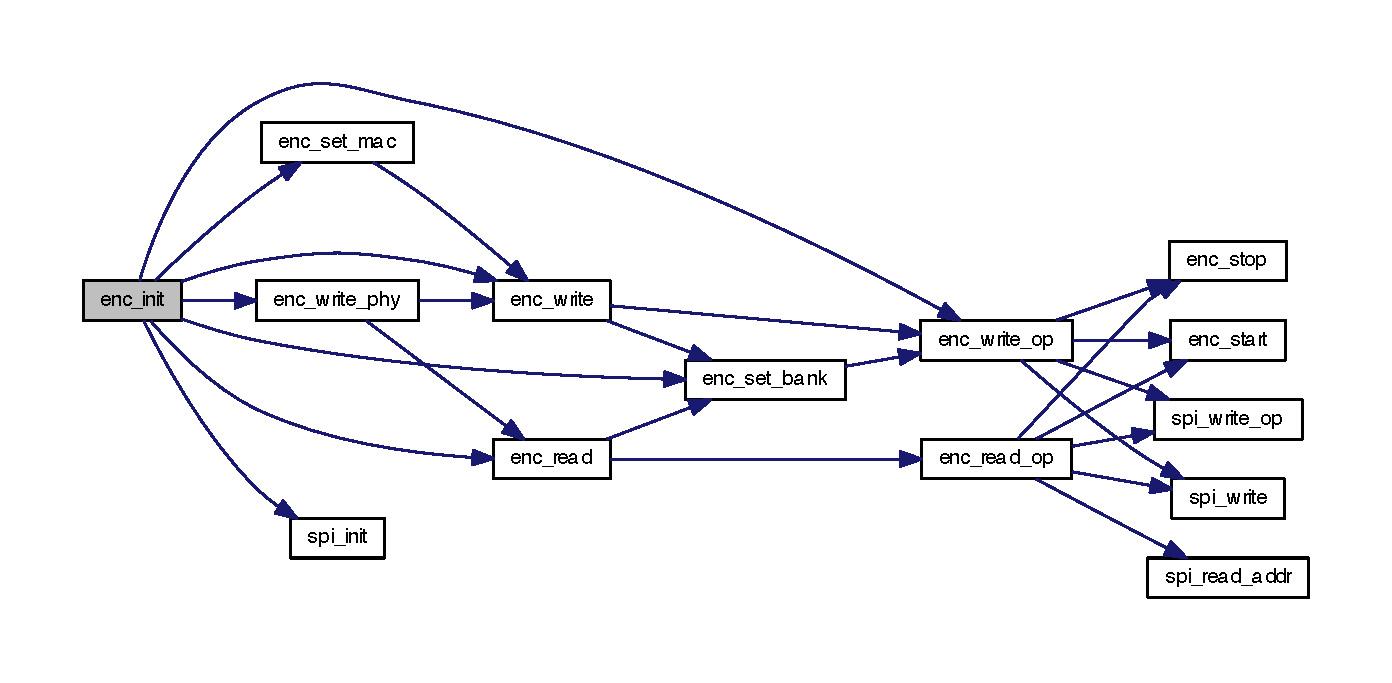
\includegraphics[width=350pt]{enc28j60_8c_a786c5765ce9469049ee56d2ca66dcf25_cgraph}
\end{center}
\end{figure}


\hypertarget{enc28j60_8c_aa75a4325284e67324bcee6b18f882b54}{\index{enc28j60.\+c@{enc28j60.\+c}!enc\+\_\+init\+\_\+phy@{enc\+\_\+init\+\_\+phy}}
\index{enc\+\_\+init\+\_\+phy@{enc\+\_\+init\+\_\+phy}!enc28j60.\+c@{enc28j60.\+c}}
\subsubsection[{enc\+\_\+init\+\_\+phy}]{\setlength{\rightskip}{0pt plus 5cm}void enc\+\_\+init\+\_\+phy (
\begin{DoxyParamCaption}
\item[{void}]{}
\end{DoxyParamCaption}
)}}\label{enc28j60_8c_aa75a4325284e67324bcee6b18f882b54}


initialize the physical interface of E\+N\+C28\+J60 



Definition at line 270 of file enc28j60.\+c.



References enc\+\_\+write\+\_\+phy(), and P\+H\+L\+C\+O\+N.



Referenced by main().



Here is the call graph for this function\+:
\nopagebreak
\begin{figure}[H]
\begin{center}
\leavevmode
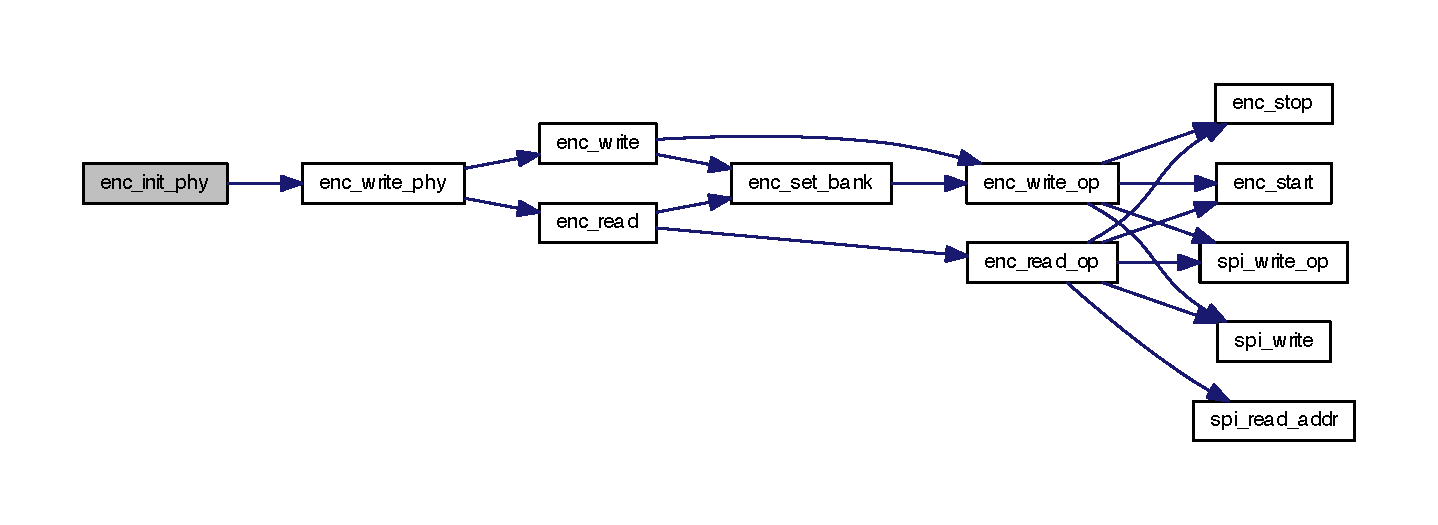
\includegraphics[width=350pt]{enc28j60_8c_aa75a4325284e67324bcee6b18f882b54_cgraph}
\end{center}
\end{figure}


\hypertarget{enc28j60_8c_a0619a7608315f0484d493da171ee37ae}{\index{enc28j60.\+c@{enc28j60.\+c}!enc\+\_\+read@{enc\+\_\+read}}
\index{enc\+\_\+read@{enc\+\_\+read}!enc28j60.\+c@{enc28j60.\+c}}
\subsubsection[{enc\+\_\+read}]{\setlength{\rightskip}{0pt plus 5cm}uint8\+\_\+t enc\+\_\+read (
\begin{DoxyParamCaption}
\item[{uint8\+\_\+t}]{addr}
\end{DoxyParamCaption}
)}}\label{enc28j60_8c_a0619a7608315f0484d493da171ee37ae}


read from from address of E\+N\+C28\+J60 


\begin{DoxyParams}{Parameters}
{\em addr} & address\\
\hline
\end{DoxyParams}
\begin{DoxyReturn}{Returns}
operation 
\end{DoxyReturn}


Definition at line 235 of file enc28j60.\+c.



References enc\+\_\+read\+\_\+op(), enc\+\_\+set\+\_\+bank(), and R\+E\+A\+D\+\_\+\+C\+T\+R\+L\+\_\+\+R\+E\+G.



Referenced by enc\+\_\+get\+\_\+rev(), enc\+\_\+init(), enc\+\_\+read\+\_\+phy(), enc\+\_\+recv\+\_\+packet(), and enc\+\_\+write\+\_\+phy().



Here is the call graph for this function\+:
\nopagebreak
\begin{figure}[H]
\begin{center}
\leavevmode
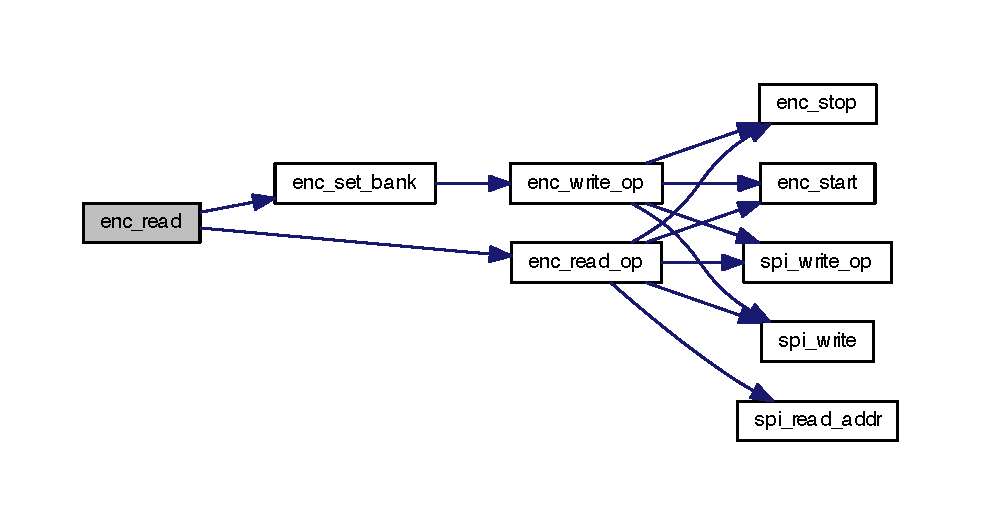
\includegraphics[width=350pt]{enc28j60_8c_a0619a7608315f0484d493da171ee37ae_cgraph}
\end{center}
\end{figure}


\hypertarget{enc28j60_8c_ae07e529513d99c8612e7878b7524109d}{\index{enc28j60.\+c@{enc28j60.\+c}!enc\+\_\+read\+\_\+buf@{enc\+\_\+read\+\_\+buf}}
\index{enc\+\_\+read\+\_\+buf@{enc\+\_\+read\+\_\+buf}!enc28j60.\+c@{enc28j60.\+c}}
\subsubsection[{enc\+\_\+read\+\_\+buf}]{\setlength{\rightskip}{0pt plus 5cm}void enc\+\_\+read\+\_\+buf (
\begin{DoxyParamCaption}
\item[{uint16\+\_\+t}]{len, }
\item[{uint8\+\_\+t $\ast$}]{data}
\end{DoxyParamCaption}
)}}\label{enc28j60_8c_ae07e529513d99c8612e7878b7524109d}


read from the buffer 


\begin{DoxyParams}{Parameters}
{\em len} & length of data \\
\hline
{\em data} & data to read \\
\hline
\end{DoxyParams}


Definition at line 295 of file enc28j60.\+c.



References enc\+\_\+start(), enc\+\_\+stop(), R\+E\+A\+D\+\_\+\+B\+U\+F\+\_\+\+M\+E\+M, spi\+\_\+read(), and spi\+\_\+write().



Referenced by enc\+\_\+recv\+\_\+packet().



Here is the call graph for this function\+:
\nopagebreak
\begin{figure}[H]
\begin{center}
\leavevmode
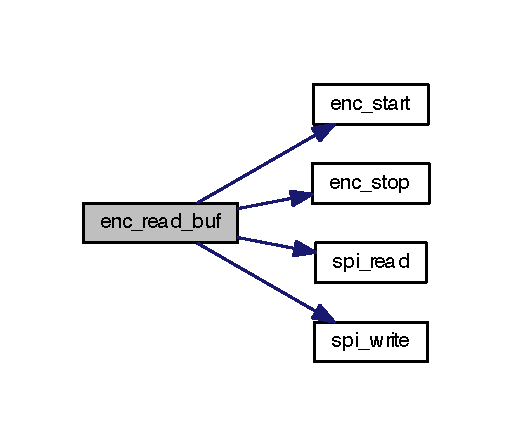
\includegraphics[width=246pt]{enc28j60_8c_ae07e529513d99c8612e7878b7524109d_cgraph}
\end{center}
\end{figure}


\hypertarget{enc28j60_8c_a28f10fce3f5c8c1e29efcce27932d149}{\index{enc28j60.\+c@{enc28j60.\+c}!enc\+\_\+read\+\_\+op@{enc\+\_\+read\+\_\+op}}
\index{enc\+\_\+read\+\_\+op@{enc\+\_\+read\+\_\+op}!enc28j60.\+c@{enc28j60.\+c}}
\subsubsection[{enc\+\_\+read\+\_\+op}]{\setlength{\rightskip}{0pt plus 5cm}uint8\+\_\+t enc\+\_\+read\+\_\+op (
\begin{DoxyParamCaption}
\item[{uint8\+\_\+t}]{op, }
\item[{uint8\+\_\+t}]{addr}
\end{DoxyParamCaption}
)}}\label{enc28j60_8c_a28f10fce3f5c8c1e29efcce27932d149}


read the operation from address of E\+N\+C28\+J60 


\begin{DoxyParams}{Parameters}
{\em op} & operation \\
\hline
{\em addr} & address\\
\hline
\end{DoxyParams}
\begin{DoxyReturn}{Returns}
data from S\+P\+I 
\end{DoxyReturn}


Definition at line 251 of file enc28j60.\+c.



References enc\+\_\+start(), enc\+\_\+stop(), spi\+\_\+read\+\_\+addr(), spi\+\_\+write(), and spi\+\_\+write\+\_\+op().



Referenced by enc\+\_\+read(), and enc\+\_\+recv\+\_\+packet().



Here is the call graph for this function\+:
\nopagebreak
\begin{figure}[H]
\begin{center}
\leavevmode
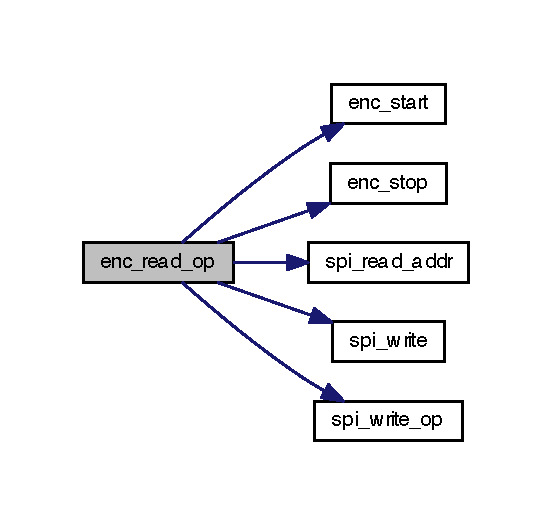
\includegraphics[width=265pt]{enc28j60_8c_a28f10fce3f5c8c1e29efcce27932d149_cgraph}
\end{center}
\end{figure}


\hypertarget{enc28j60_8c_ab1b8f7c1f5dbcb0e500da8ed87219cd7}{\index{enc28j60.\+c@{enc28j60.\+c}!enc\+\_\+read\+\_\+phy@{enc\+\_\+read\+\_\+phy}}
\index{enc\+\_\+read\+\_\+phy@{enc\+\_\+read\+\_\+phy}!enc28j60.\+c@{enc28j60.\+c}}
\subsubsection[{enc\+\_\+read\+\_\+phy}]{\setlength{\rightskip}{0pt plus 5cm}uint16\+\_\+t enc\+\_\+read\+\_\+phy (
\begin{DoxyParamCaption}
\item[{uint8\+\_\+t}]{addr}
\end{DoxyParamCaption}
)}}\label{enc28j60_8c_ab1b8f7c1f5dbcb0e500da8ed87219cd7}


read from physical address of E\+N\+C28\+J60 


\begin{DoxyParams}{Parameters}
{\em addr} & address\\
\hline
\end{DoxyParams}
\begin{DoxyReturn}{Returns}
data 
\end{DoxyReturn}


Definition at line 209 of file enc28j60.\+c.



References B\+U\+S\+Y, enc\+\_\+read(), enc\+\_\+write(), M\+I\+C\+M\+D, M\+I\+I\+R\+D, M\+I\+R\+D\+H, M\+I\+R\+D\+L, M\+I\+R\+E\+G\+A\+D\+R, and M\+I\+S\+T\+A\+T.



Here is the call graph for this function\+:
\nopagebreak
\begin{figure}[H]
\begin{center}
\leavevmode
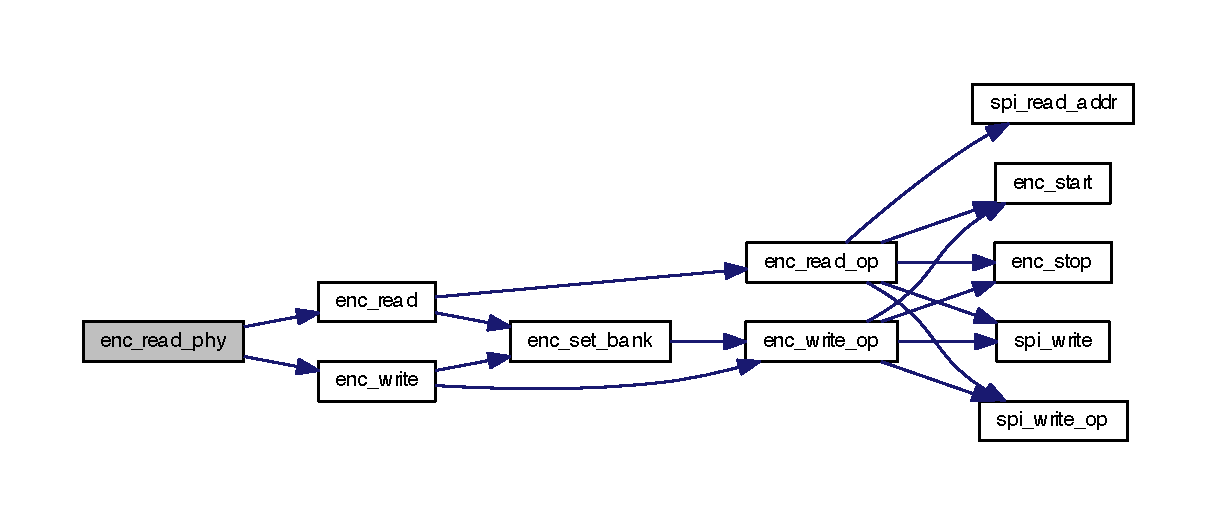
\includegraphics[width=350pt]{enc28j60_8c_ab1b8f7c1f5dbcb0e500da8ed87219cd7_cgraph}
\end{center}
\end{figure}


\hypertarget{enc28j60_8c_a412f11a9dbdb9cf9bf812751044f4d4f}{\index{enc28j60.\+c@{enc28j60.\+c}!enc\+\_\+recv\+\_\+packet@{enc\+\_\+recv\+\_\+packet}}
\index{enc\+\_\+recv\+\_\+packet@{enc\+\_\+recv\+\_\+packet}!enc28j60.\+c@{enc28j60.\+c}}
\subsubsection[{enc\+\_\+recv\+\_\+packet}]{\setlength{\rightskip}{0pt plus 5cm}uint16\+\_\+t enc\+\_\+recv\+\_\+packet (
\begin{DoxyParamCaption}
\item[{uint16\+\_\+t}]{maxlen, }
\item[{uint8\+\_\+t $\ast$}]{packet}
\end{DoxyParamCaption}
)}}\label{enc28j60_8c_a412f11a9dbdb9cf9bf812751044f4d4f}


receive a packet from ethernet 


\begin{DoxyParams}{Parameters}
{\em maxlen} & maximum length of packet to receive \\
\hline
{\em packet} & packet to receive\\
\hline
\end{DoxyParams}
\begin{DoxyReturn}{Returns}
length of received packet 
\end{DoxyReturn}


Definition at line 368 of file enc28j60.\+c.



References B\+I\+T\+\_\+\+F\+I\+E\+L\+D\+\_\+\+S\+E\+T, E\+C\+O\+N2, enc\+\_\+read(), enc\+\_\+read\+\_\+buf(), enc\+\_\+read\+\_\+op(), enc\+\_\+write(), enc\+\_\+write\+\_\+op(), E\+P\+K\+T\+C\+N\+T, E\+R\+D\+P\+T\+H, E\+R\+D\+P\+T\+L, E\+R\+X\+R\+D\+P\+T\+H, E\+R\+X\+R\+D\+P\+T\+L, M\+I\+N, p\+\_\+next, P\+K\+T\+D\+E\+C, and R\+E\+A\+D\+\_\+\+B\+U\+F\+\_\+\+M\+E\+M.



Referenced by main().



Here is the call graph for this function\+:
\nopagebreak
\begin{figure}[H]
\begin{center}
\leavevmode
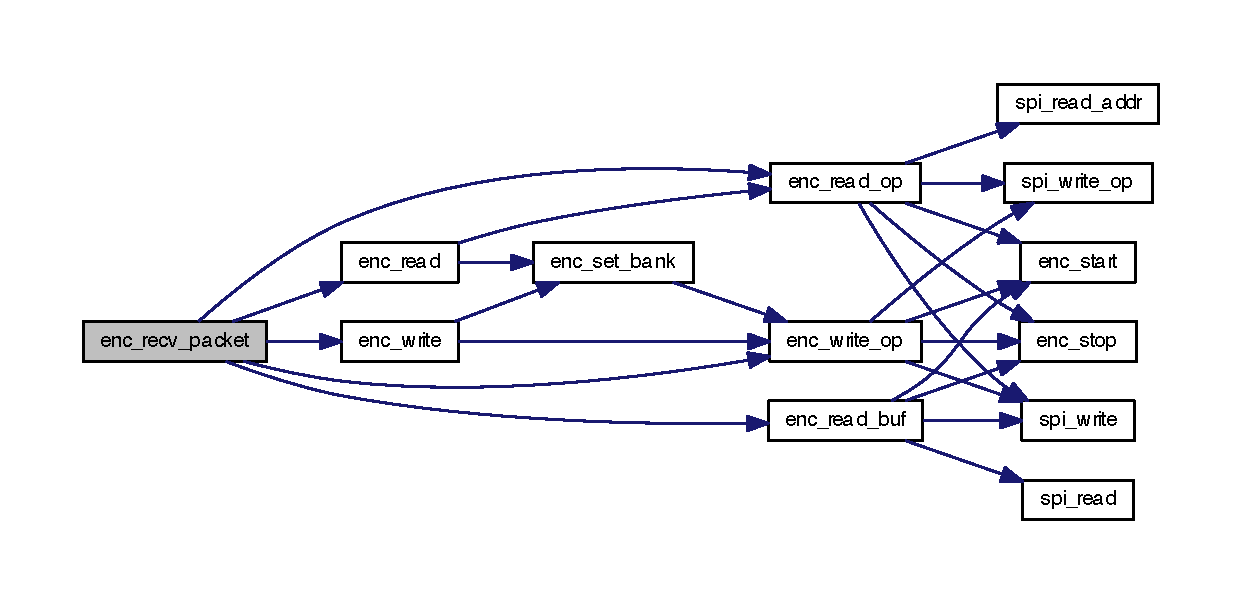
\includegraphics[width=350pt]{enc28j60_8c_a412f11a9dbdb9cf9bf812751044f4d4f_cgraph}
\end{center}
\end{figure}


\hypertarget{enc28j60_8c_a094a800fcadc3033c6d1e90d2eecba23}{\index{enc28j60.\+c@{enc28j60.\+c}!enc\+\_\+send\+\_\+packet@{enc\+\_\+send\+\_\+packet}}
\index{enc\+\_\+send\+\_\+packet@{enc\+\_\+send\+\_\+packet}!enc28j60.\+c@{enc28j60.\+c}}
\subsubsection[{enc\+\_\+send\+\_\+packet}]{\setlength{\rightskip}{0pt plus 5cm}void enc\+\_\+send\+\_\+packet (
\begin{DoxyParamCaption}
\item[{uint16\+\_\+t}]{len, }
\item[{uint8\+\_\+t $\ast$}]{packet}
\end{DoxyParamCaption}
)}}\label{enc28j60_8c_a094a800fcadc3033c6d1e90d2eecba23}


send a packet to ethernet 


\begin{DoxyParams}{Parameters}
{\em len} & length of packet \\
\hline
{\em packet} & packet to send \\
\hline
\end{DoxyParams}


Definition at line 344 of file enc28j60.\+c.



References B\+I\+T\+\_\+\+F\+I\+E\+L\+D\+\_\+\+S\+E\+T, E\+C\+O\+N1, enc\+\_\+write(), enc\+\_\+write\+\_\+buf(), enc\+\_\+write\+\_\+op(), E\+T\+X\+N\+D\+H, E\+T\+X\+N\+D\+L, E\+W\+R\+P\+T\+H, E\+W\+R\+P\+T\+L, T\+X\+\_\+\+S\+T\+A\+R\+T\+\_\+\+I\+N\+I\+T, T\+X\+R\+T\+S, and W\+R\+I\+T\+E\+\_\+\+B\+U\+F\+\_\+\+M\+E\+M.



Referenced by arp\+\_\+answer(), echo\+\_\+reply(), and udp\+\_\+reply().



Here is the call graph for this function\+:
\nopagebreak
\begin{figure}[H]
\begin{center}
\leavevmode
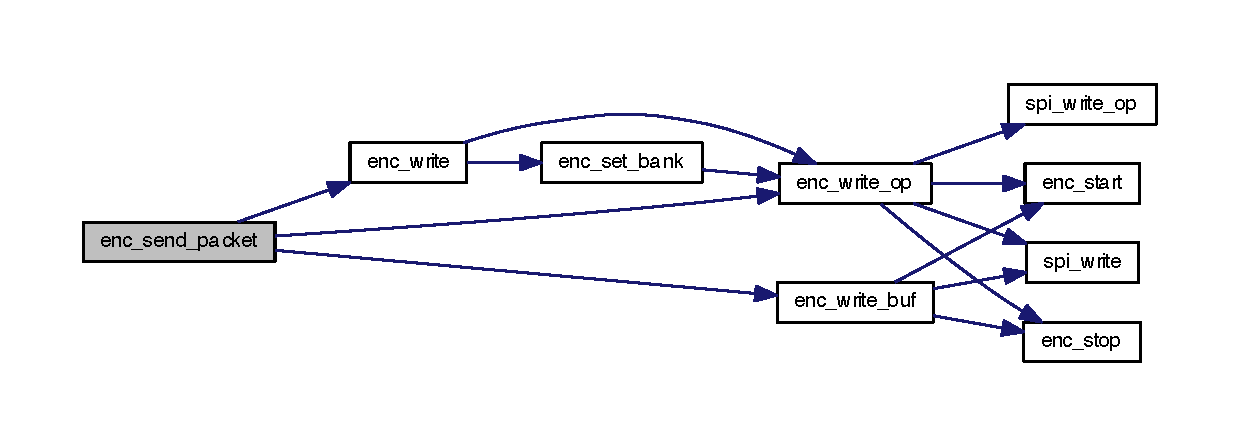
\includegraphics[width=350pt]{enc28j60_8c_a094a800fcadc3033c6d1e90d2eecba23_cgraph}
\end{center}
\end{figure}


\hypertarget{enc28j60_8c_ac175ce9462129e5d35f06935aa42c9f6}{\index{enc28j60.\+c@{enc28j60.\+c}!enc\+\_\+set\+\_\+bank@{enc\+\_\+set\+\_\+bank}}
\index{enc\+\_\+set\+\_\+bank@{enc\+\_\+set\+\_\+bank}!enc28j60.\+c@{enc28j60.\+c}}
\subsubsection[{enc\+\_\+set\+\_\+bank}]{\setlength{\rightskip}{0pt plus 5cm}void enc\+\_\+set\+\_\+bank (
\begin{DoxyParamCaption}
\item[{uint8\+\_\+t}]{addr}
\end{DoxyParamCaption}
)}}\label{enc28j60_8c_ac175ce9462129e5d35f06935aa42c9f6}


set the bank on address 


\begin{DoxyParams}{Parameters}
{\em addr} & address to set \\
\hline
\end{DoxyParams}


Definition at line 174 of file enc28j60.\+c.



References A\+D\+D\+R\+\_\+\+M\+A\+S\+K, B\+A\+N\+K\+\_\+\+M\+A\+S\+K, B\+I\+T\+\_\+\+F\+I\+E\+L\+D\+\_\+\+C\+L\+R, B\+I\+T\+\_\+\+F\+I\+E\+L\+D\+\_\+\+S\+E\+T, B\+S\+E\+L0, B\+S\+E\+L1, E\+C\+O\+N1, enc\+\_\+bank, and enc\+\_\+write\+\_\+op().



Referenced by enc\+\_\+init(), enc\+\_\+read(), and enc\+\_\+write().



Here is the call graph for this function\+:
\nopagebreak
\begin{figure}[H]
\begin{center}
\leavevmode
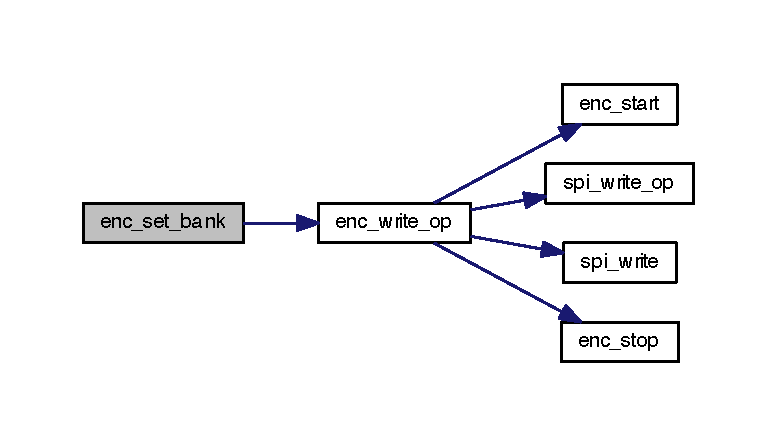
\includegraphics[width=350pt]{enc28j60_8c_ac175ce9462129e5d35f06935aa42c9f6_cgraph}
\end{center}
\end{figure}


\hypertarget{enc28j60_8c_a3de012f2c3b25ad182f94f5b1ab9a771}{\index{enc28j60.\+c@{enc28j60.\+c}!enc\+\_\+set\+\_\+mac@{enc\+\_\+set\+\_\+mac}}
\index{enc\+\_\+set\+\_\+mac@{enc\+\_\+set\+\_\+mac}!enc28j60.\+c@{enc28j60.\+c}}
\subsubsection[{enc\+\_\+set\+\_\+mac}]{\setlength{\rightskip}{0pt plus 5cm}void enc\+\_\+set\+\_\+mac (
\begin{DoxyParamCaption}
\item[{uint8\+\_\+t}]{mymac\mbox{[}$\,$\mbox{]}}
\end{DoxyParamCaption}
)}}\label{enc28j60_8c_a3de012f2c3b25ad182f94f5b1ab9a771}


set the mac-\/address to B\+A\+N\+K3 register 


\begin{DoxyParams}{Parameters}
{\em mymac\mbox{[}$\,$\mbox{]}} & my mac address \\
\hline
\end{DoxyParams}


Definition at line 58 of file enc28j60.\+c.



References enc\+\_\+write(), M\+A\+A\+D\+R0, M\+A\+A\+D\+R1, M\+A\+A\+D\+R2, M\+A\+A\+D\+R3, M\+A\+A\+D\+R4, and M\+A\+A\+D\+R5.



Referenced by enc\+\_\+init().



Here is the call graph for this function\+:
\nopagebreak
\begin{figure}[H]
\begin{center}
\leavevmode
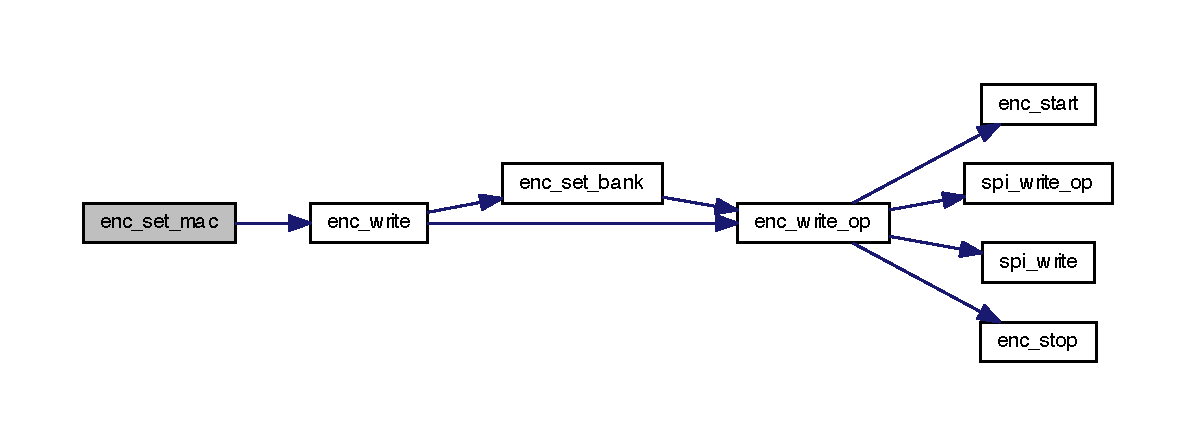
\includegraphics[width=350pt]{enc28j60_8c_a3de012f2c3b25ad182f94f5b1ab9a771_cgraph}
\end{center}
\end{figure}


\hypertarget{enc28j60_8c_a6ae6915ab4363819a3492bd8509263e5}{\index{enc28j60.\+c@{enc28j60.\+c}!enc\+\_\+start@{enc\+\_\+start}}
\index{enc\+\_\+start@{enc\+\_\+start}!enc28j60.\+c@{enc28j60.\+c}}
\subsubsection[{enc\+\_\+start}]{\setlength{\rightskip}{0pt plus 5cm}void enc\+\_\+start (
\begin{DoxyParamCaption}
\item[{void}]{}
\end{DoxyParamCaption}
)}}\label{enc28j60_8c_a6ae6915ab4363819a3492bd8509263e5}


start E\+N\+C28\+J60 pin to write or to read 



Definition at line 38 of file enc28j60.\+c.



References E\+N\+C\+\_\+\+C\+T\+R\+L\+\_\+\+C\+S, and E\+N\+C\+\_\+\+C\+T\+R\+L\+\_\+\+P\+O\+R\+T.



Referenced by enc\+\_\+read\+\_\+buf(), enc\+\_\+read\+\_\+op(), enc\+\_\+write\+\_\+buf(), and enc\+\_\+write\+\_\+op().

\hypertarget{enc28j60_8c_a63e6002e7cdb7ac2433fcb6fb4fc0b16}{\index{enc28j60.\+c@{enc28j60.\+c}!enc\+\_\+stop@{enc\+\_\+stop}}
\index{enc\+\_\+stop@{enc\+\_\+stop}!enc28j60.\+c@{enc28j60.\+c}}
\subsubsection[{enc\+\_\+stop}]{\setlength{\rightskip}{0pt plus 5cm}void enc\+\_\+stop (
\begin{DoxyParamCaption}
\item[{void}]{}
\end{DoxyParamCaption}
)}}\label{enc28j60_8c_a63e6002e7cdb7ac2433fcb6fb4fc0b16}


stop the E\+N\+C28\+J60 pin 



Definition at line 47 of file enc28j60.\+c.



References E\+N\+C\+\_\+\+C\+T\+R\+L\+\_\+\+C\+S, and E\+N\+C\+\_\+\+C\+T\+R\+L\+\_\+\+P\+O\+R\+T.



Referenced by enc\+\_\+read\+\_\+buf(), enc\+\_\+read\+\_\+op(), enc\+\_\+write\+\_\+buf(), and enc\+\_\+write\+\_\+op().

\hypertarget{enc28j60_8c_a7520f33b52393de8d0e3caa796e0baa2}{\index{enc28j60.\+c@{enc28j60.\+c}!enc\+\_\+write@{enc\+\_\+write}}
\index{enc\+\_\+write@{enc\+\_\+write}!enc28j60.\+c@{enc28j60.\+c}}
\subsubsection[{enc\+\_\+write}]{\setlength{\rightskip}{0pt plus 5cm}void enc\+\_\+write (
\begin{DoxyParamCaption}
\item[{uint8\+\_\+t}]{addr, }
\item[{uint8\+\_\+t}]{data}
\end{DoxyParamCaption}
)}}\label{enc28j60_8c_a7520f33b52393de8d0e3caa796e0baa2}


write on E\+N\+C28\+J60 


\begin{DoxyParams}{Parameters}
{\em addr} & address to write \\
\hline
{\em data} & data to send \\
\hline
\end{DoxyParams}


Definition at line 162 of file enc28j60.\+c.



References enc\+\_\+set\+\_\+bank(), enc\+\_\+write\+\_\+op(), and W\+R\+I\+T\+E\+\_\+\+C\+T\+R\+L\+\_\+\+R\+E\+G.



Referenced by enc\+\_\+init(), enc\+\_\+read\+\_\+phy(), enc\+\_\+recv\+\_\+packet(), enc\+\_\+send\+\_\+packet(), enc\+\_\+set\+\_\+mac(), and enc\+\_\+write\+\_\+phy().



Here is the call graph for this function\+:
\nopagebreak
\begin{figure}[H]
\begin{center}
\leavevmode
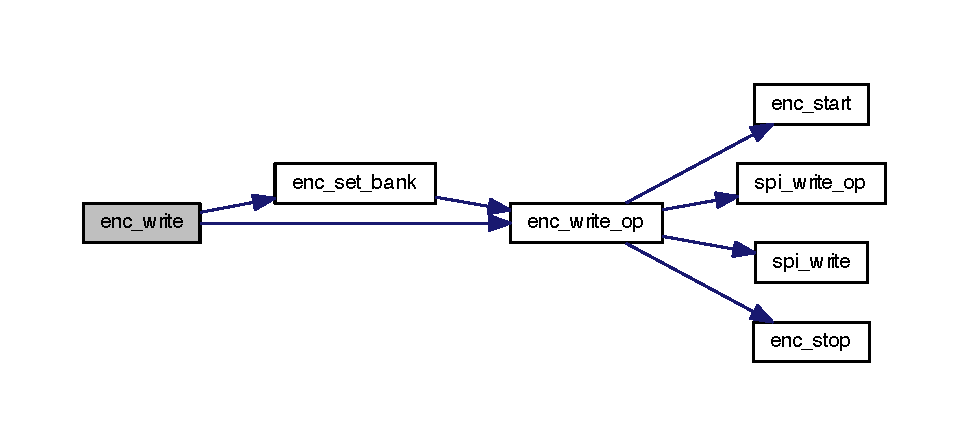
\includegraphics[width=350pt]{enc28j60_8c_a7520f33b52393de8d0e3caa796e0baa2_cgraph}
\end{center}
\end{figure}


\hypertarget{enc28j60_8c_a8ae17d4efc162d054952cc4cb80d422c}{\index{enc28j60.\+c@{enc28j60.\+c}!enc\+\_\+write\+\_\+buf@{enc\+\_\+write\+\_\+buf}}
\index{enc\+\_\+write\+\_\+buf@{enc\+\_\+write\+\_\+buf}!enc28j60.\+c@{enc28j60.\+c}}
\subsubsection[{enc\+\_\+write\+\_\+buf}]{\setlength{\rightskip}{0pt plus 5cm}void enc\+\_\+write\+\_\+buf (
\begin{DoxyParamCaption}
\item[{uint16\+\_\+t}]{len, }
\item[{uint8\+\_\+t $\ast$}]{data}
\end{DoxyParamCaption}
)}}\label{enc28j60_8c_a8ae17d4efc162d054952cc4cb80d422c}


write the buffer 


\begin{DoxyParams}{Parameters}
{\em len} & length of data \\
\hline
{\em data} & data \\
\hline
\end{DoxyParams}


Definition at line 314 of file enc28j60.\+c.



References enc\+\_\+start(), enc\+\_\+stop(), spi\+\_\+write(), and W\+R\+I\+T\+E\+\_\+\+B\+U\+F\+\_\+\+M\+E\+M.



Referenced by enc\+\_\+send\+\_\+packet().



Here is the call graph for this function\+:
\nopagebreak
\begin{figure}[H]
\begin{center}
\leavevmode
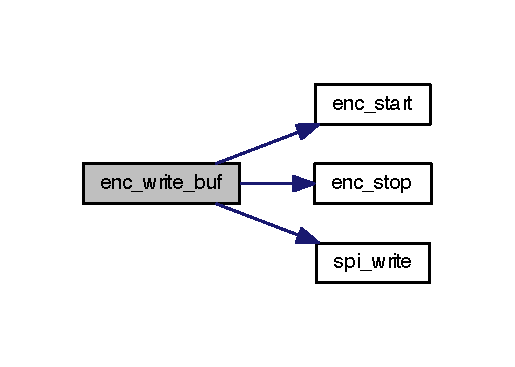
\includegraphics[width=247pt]{enc28j60_8c_a8ae17d4efc162d054952cc4cb80d422c_cgraph}
\end{center}
\end{figure}


\hypertarget{enc28j60_8c_ab64d8270b5a710a2ff635d4449c91a08}{\index{enc28j60.\+c@{enc28j60.\+c}!enc\+\_\+write\+\_\+op@{enc\+\_\+write\+\_\+op}}
\index{enc\+\_\+write\+\_\+op@{enc\+\_\+write\+\_\+op}!enc28j60.\+c@{enc28j60.\+c}}
\subsubsection[{enc\+\_\+write\+\_\+op}]{\setlength{\rightskip}{0pt plus 5cm}void enc\+\_\+write\+\_\+op (
\begin{DoxyParamCaption}
\item[{uint8\+\_\+t}]{op, }
\item[{uint8\+\_\+t}]{addr, }
\item[{uint8\+\_\+t}]{data}
\end{DoxyParamCaption}
)}}\label{enc28j60_8c_ab64d8270b5a710a2ff635d4449c91a08}


write the operation 


\begin{DoxyParams}{Parameters}
{\em op} & operation to write on S\+P\+I \\
\hline
{\em addr} & address to write \\
\hline
{\em data} & data to send on S\+P\+I \\
\hline
\end{DoxyParams}


Definition at line 145 of file enc28j60.\+c.



References enc\+\_\+start(), enc\+\_\+stop(), spi\+\_\+write(), and spi\+\_\+write\+\_\+op().



Referenced by enc\+\_\+init(), enc\+\_\+recv\+\_\+packet(), enc\+\_\+send\+\_\+packet(), enc\+\_\+set\+\_\+bank(), and enc\+\_\+write().



Here is the call graph for this function\+:
\nopagebreak
\begin{figure}[H]
\begin{center}
\leavevmode
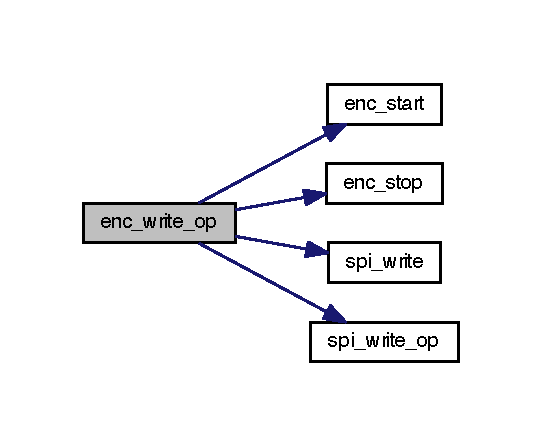
\includegraphics[width=260pt]{enc28j60_8c_ab64d8270b5a710a2ff635d4449c91a08_cgraph}
\end{center}
\end{figure}


\hypertarget{enc28j60_8c_ab6908af0f98d4b54d35cbcd699119346}{\index{enc28j60.\+c@{enc28j60.\+c}!enc\+\_\+write\+\_\+phy@{enc\+\_\+write\+\_\+phy}}
\index{enc\+\_\+write\+\_\+phy@{enc\+\_\+write\+\_\+phy}!enc28j60.\+c@{enc28j60.\+c}}
\subsubsection[{enc\+\_\+write\+\_\+phy}]{\setlength{\rightskip}{0pt plus 5cm}void enc\+\_\+write\+\_\+phy (
\begin{DoxyParamCaption}
\item[{uint8\+\_\+t}]{addr, }
\item[{uint16\+\_\+t}]{data}
\end{DoxyParamCaption}
)}}\label{enc28j60_8c_ab6908af0f98d4b54d35cbcd699119346}


write the data on E\+N\+C28\+J60 physical address 


\begin{DoxyParams}{Parameters}
{\em addr} & address \\
\hline
{\em data} & data \\
\hline
\end{DoxyParams}


Definition at line 190 of file enc28j60.\+c.



References B\+U\+S\+Y, enc\+\_\+read(), enc\+\_\+write(), M\+I\+R\+E\+G\+A\+D\+R, M\+I\+S\+T\+A\+T, M\+I\+W\+R\+H, and M\+I\+W\+R\+L.



Referenced by enc\+\_\+init(), and enc\+\_\+init\+\_\+phy().



Here is the call graph for this function\+:
\nopagebreak
\begin{figure}[H]
\begin{center}
\leavevmode
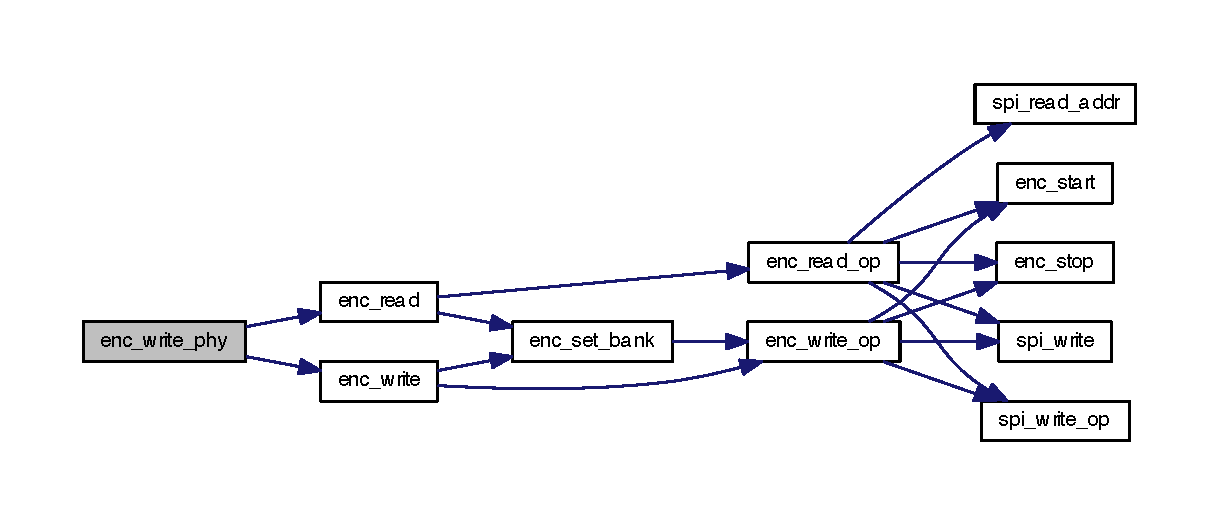
\includegraphics[width=350pt]{enc28j60_8c_ab6908af0f98d4b54d35cbcd699119346_cgraph}
\end{center}
\end{figure}




\subsection{Variable Documentation}
\hypertarget{enc28j60_8c_a8cf887c83e16783a97183adf9b0bd5eb}{\index{enc28j60.\+c@{enc28j60.\+c}!enc\+\_\+bank@{enc\+\_\+bank}}
\index{enc\+\_\+bank@{enc\+\_\+bank}!enc28j60.\+c@{enc28j60.\+c}}
\subsubsection[{enc\+\_\+bank}]{\setlength{\rightskip}{0pt plus 5cm}uint8\+\_\+t enc\+\_\+bank}}\label{enc28j60_8c_a8cf887c83e16783a97183adf9b0bd5eb}


Definition at line 31 of file enc28j60.\+c.



Referenced by enc\+\_\+set\+\_\+bank().

\hypertarget{enc28j60_8c_ad7e304a214204367dd0528e5df3c59f0}{\index{enc28j60.\+c@{enc28j60.\+c}!p\+\_\+next@{p\+\_\+next}}
\index{p\+\_\+next@{p\+\_\+next}!enc28j60.\+c@{enc28j60.\+c}}
\subsubsection[{p\+\_\+next}]{\setlength{\rightskip}{0pt plus 5cm}unsigned int p\+\_\+next}}\label{enc28j60_8c_ad7e304a214204367dd0528e5df3c59f0}


Definition at line 32 of file enc28j60.\+c.



Referenced by enc\+\_\+init(), and enc\+\_\+recv\+\_\+packet().


\hypertarget{icp_8c}{\section{driver/icp.c File Reference}
\label{icp_8c}\index{driver/icp.\+c@{driver/icp.\+c}}
}


driver for input capture pin operations  


{\ttfamily \#include $<$driver/leds.\+h$>$}\\*
{\ttfamily \#include $<$driver/icp.\+h$>$}\\*
Include dependency graph for icp.\+c\+:
\nopagebreak
\begin{figure}[H]
\begin{center}
\leavevmode
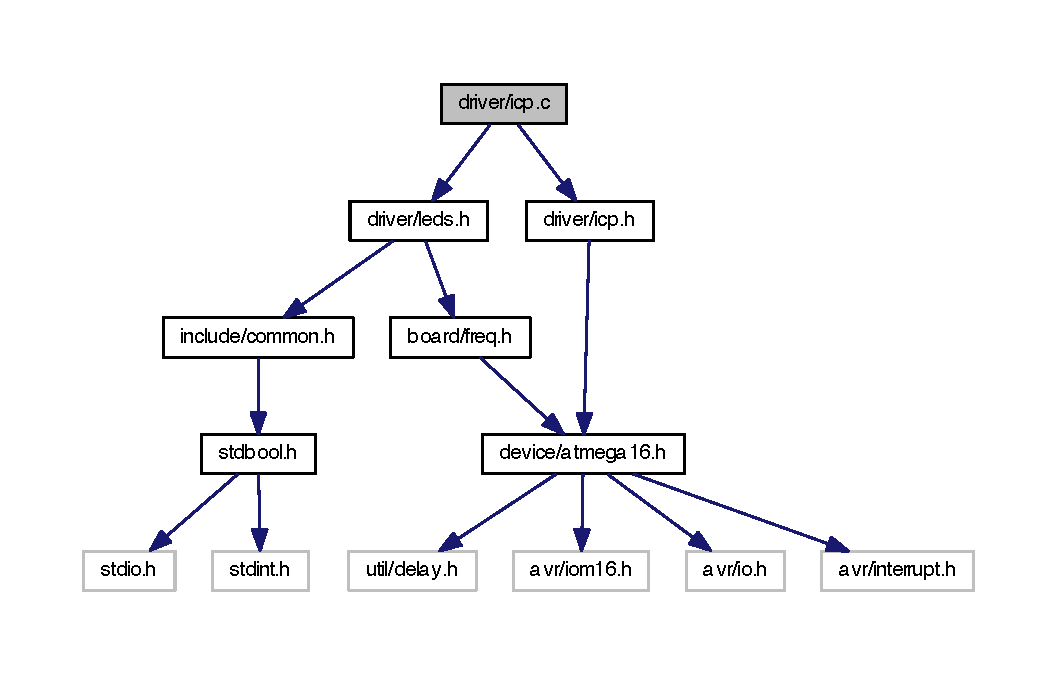
\includegraphics[width=350pt]{icp_8c__incl}
\end{center}
\end{figure}
\subsection*{Functions}
\begin{DoxyCompactItemize}
\item 
void \hyperlink{icp_8c_a9aea3198ad5628ffd740d6dc46d0f640}{icp\+\_\+init} (void($\ast$call\+\_\+back)(uint16\+\_\+t))
\begin{DoxyCompactList}\small\item\em initialize the input capture pin on timer 1 \end{DoxyCompactList}\item 
\hyperlink{icp_8c_a5da59e05fa5ade4be7c7656aee78291a}{I\+S\+R} (T\+I\+M\+E\+R1\+\_\+\+C\+A\+P\+T\+\_\+vect)
\begin{DoxyCompactList}\small\item\em Timer1 Input Capture Interrupt. \end{DoxyCompactList}\end{DoxyCompactItemize}


\subsection{Detailed Description}
driver for input capture pin operations 

\begin{DoxyAuthor}{Author}
M. Ozgan, \href{mailto:mozgan@mozgan.org}{\tt mozgan@mozgan.\+org} 
\end{DoxyAuthor}
\begin{DoxyVersion}{Version}
0.\+1 
\end{DoxyVersion}
\begin{DoxyDate}{Date}
22.\+08.\+2013 15\+:57\+:28 
\end{DoxyDate}
\begin{DoxyParagraph}{Compiler}
gcc (on Mac, and 4.\+4\+B\+S\+D) 
\end{DoxyParagraph}
\begin{DoxyParagraph}{Company}
T\+U Wien 
\end{DoxyParagraph}


\begin{DoxyRefDesc}{Bug}
\item[\hyperlink{bug__bug000005}{Bug}]none \end{DoxyRefDesc}
\begin{DoxyRefDesc}{Todo}
\item[\hyperlink{todo__todo000005}{Todo}]none \end{DoxyRefDesc}


Definition in file \hyperlink{icp_8c_source}{icp.\+c}.



\subsection{Function Documentation}
\hypertarget{icp_8c_a9aea3198ad5628ffd740d6dc46d0f640}{\index{icp.\+c@{icp.\+c}!icp\+\_\+init@{icp\+\_\+init}}
\index{icp\+\_\+init@{icp\+\_\+init}!icp.\+c@{icp.\+c}}
\subsubsection[{icp\+\_\+init}]{\setlength{\rightskip}{0pt plus 5cm}void icp\+\_\+init (
\begin{DoxyParamCaption}
\item[{void($\ast$)(uint16\+\_\+t)}]{call\+\_\+back}
\end{DoxyParamCaption}
)}}\label{icp_8c_a9aea3198ad5628ffd740d6dc46d0f640}


initialize the input capture pin on timer 1 


\begin{DoxyParams}{Parameters}
{\em call\+\_\+back} & call back function from interrupt to call \\
\hline
\end{DoxyParams}


Definition at line 36 of file icp.\+c.



References F\+\_\+\+C\+P\+U, icp\+\_\+handler, and N\+U\+L\+L.



Referenced by main().

\hypertarget{icp_8c_a5da59e05fa5ade4be7c7656aee78291a}{\index{icp.\+c@{icp.\+c}!I\+S\+R@{I\+S\+R}}
\index{I\+S\+R@{I\+S\+R}!icp.\+c@{icp.\+c}}
\subsubsection[{I\+S\+R}]{\setlength{\rightskip}{0pt plus 5cm}I\+S\+R (
\begin{DoxyParamCaption}
\item[{T\+I\+M\+E\+R1\+\_\+\+C\+A\+P\+T\+\_\+vect}]{}
\end{DoxyParamCaption}
)}}\label{icp_8c_a5da59e05fa5ade4be7c7656aee78291a}


Timer1 Input Capture Interrupt. 


\begin{DoxyParams}{Parameters}
{\em T\+I\+M\+E\+R1\+\_\+\+C\+A\+P\+T\+\_\+vect} & interrupt name \\
\hline
\end{DoxyParams}


Definition at line 86 of file icp.\+c.



References icp\+\_\+handler, and N\+U\+L\+L.


\hypertarget{icp_8h}{\section{driver/icp.h File Reference}
\label{icp_8h}\index{driver/icp.\+h@{driver/icp.\+h}}
}


header file for input capture pin operations  


{\ttfamily \#include $<$device/atmega16.\+h$>$}\\*
Include dependency graph for icp.\+h\+:
\nopagebreak
\begin{figure}[H]
\begin{center}
\leavevmode
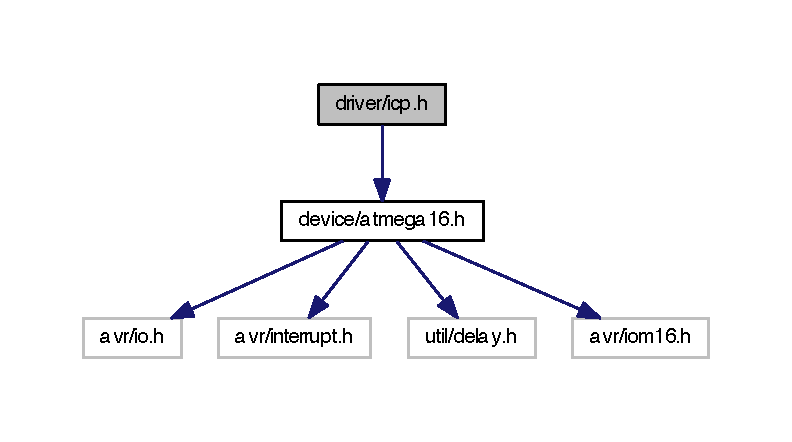
\includegraphics[width=350pt]{icp_8h__incl}
\end{center}
\end{figure}
This graph shows which files directly or indirectly include this file\+:
\nopagebreak
\begin{figure}[H]
\begin{center}
\leavevmode
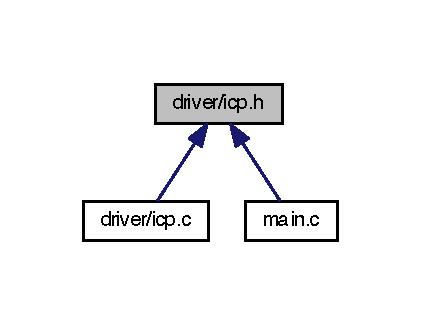
\includegraphics[width=202pt]{icp_8h__dep__incl}
\end{center}
\end{figure}
\subsection*{Functions}
\begin{DoxyCompactItemize}
\item 
void \hyperlink{icp_8h_ae5e07be4f0f76ab7430624248ad51771}{icp\+\_\+init} (void($\ast$)(uint16\+\_\+t))
\begin{DoxyCompactList}\small\item\em initialize the input capture pin on timer 1 \end{DoxyCompactList}\end{DoxyCompactItemize}
\subsection*{Variables}
\begin{DoxyCompactItemize}
\item 
void($\ast$ \hyperlink{icp_8h_a7da0b6c4aa82795dc56e20bc06f8f9d3}{icp\+\_\+handler} )(uint16\+\_\+t)
\end{DoxyCompactItemize}


\subsection{Detailed Description}
header file for input capture pin operations 

\begin{DoxyAuthor}{Author}
M. Ozgan, \href{mailto:mozgan@mozgan.org}{\tt mozgan@mozgan.\+org} 
\end{DoxyAuthor}
\begin{DoxyVersion}{Version}
0.\+1 
\end{DoxyVersion}
\begin{DoxyDate}{Date}
22.\+08.\+2013 15\+:56\+:37 
\end{DoxyDate}
\begin{DoxyParagraph}{Compiler}
gcc (on Mac, and 4.\+4\+B\+S\+D) 
\end{DoxyParagraph}
\begin{DoxyParagraph}{Company}
T\+U Wien 
\end{DoxyParagraph}


\begin{DoxyRefDesc}{Bug}
\item[\hyperlink{bug__bug000006}{Bug}]none \end{DoxyRefDesc}
\begin{DoxyRefDesc}{Todo}
\item[\hyperlink{todo__todo000006}{Todo}]none \end{DoxyRefDesc}


Definition in file \hyperlink{icp_8h_source}{icp.\+h}.



\subsection{Function Documentation}
\hypertarget{icp_8h_ae5e07be4f0f76ab7430624248ad51771}{\index{icp.\+h@{icp.\+h}!icp\+\_\+init@{icp\+\_\+init}}
\index{icp\+\_\+init@{icp\+\_\+init}!icp.\+h@{icp.\+h}}
\subsubsection[{icp\+\_\+init}]{\setlength{\rightskip}{0pt plus 5cm}void icp\+\_\+init (
\begin{DoxyParamCaption}
\item[{void($\ast$)(uint16\+\_\+t)}]{call\+\_\+back}
\end{DoxyParamCaption}
)}}\label{icp_8h_ae5e07be4f0f76ab7430624248ad51771}


initialize the input capture pin on timer 1 


\begin{DoxyParams}{Parameters}
{\em call\+\_\+back} & call back function from interrupt to call \\
\hline
\end{DoxyParams}


Definition at line 36 of file icp.\+c.



References F\+\_\+\+C\+P\+U, icp\+\_\+handler, and N\+U\+L\+L.



Referenced by main().



\subsection{Variable Documentation}
\hypertarget{icp_8h_a7da0b6c4aa82795dc56e20bc06f8f9d3}{\index{icp.\+h@{icp.\+h}!icp\+\_\+handler@{icp\+\_\+handler}}
\index{icp\+\_\+handler@{icp\+\_\+handler}!icp.\+h@{icp.\+h}}
\subsubsection[{icp\+\_\+handler}]{\setlength{\rightskip}{0pt plus 5cm}void($\ast$ icp\+\_\+handler)(uint16\+\_\+t)}}\label{icp_8h_a7da0b6c4aa82795dc56e20bc06f8f9d3}
call back function 

Definition at line 34 of file icp.\+h.



Referenced by icp\+\_\+init(), and I\+S\+R().


\hypertarget{leds_8c}{\section{driver/leds.c File Reference}
\label{leds_8c}\index{driver/leds.\+c@{driver/leds.\+c}}
}


driver for leds (to use for debugging)  


{\ttfamily \#include $<$driver/leds.\+h$>$}\\*
Include dependency graph for leds.\+c\+:
\nopagebreak
\begin{figure}[H]
\begin{center}
\leavevmode
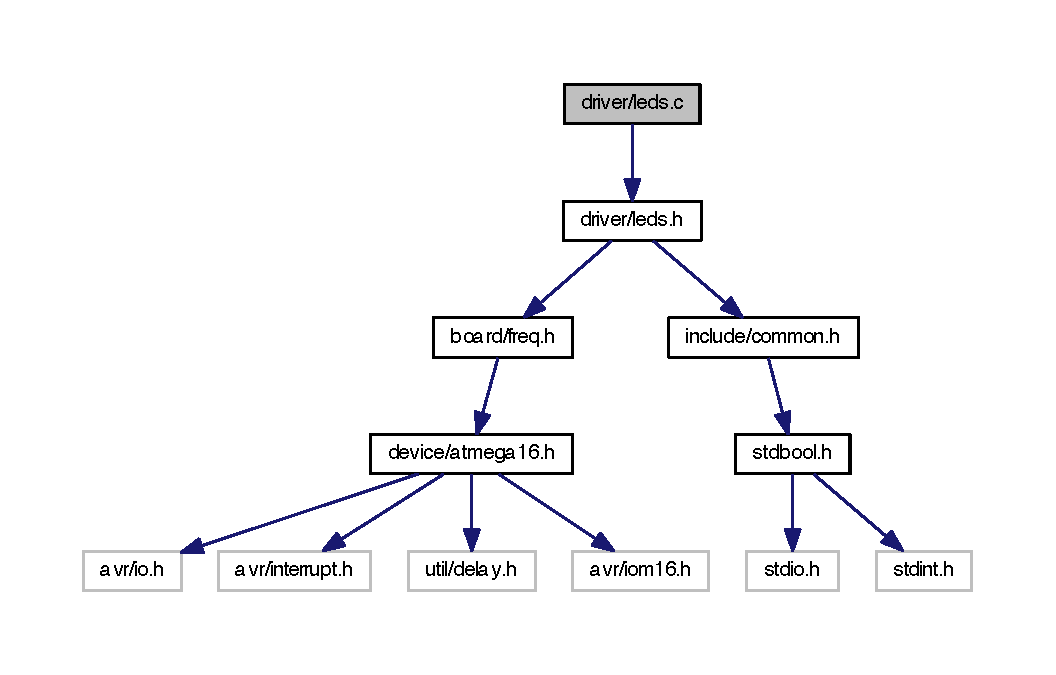
\includegraphics[width=350pt]{leds_8c__incl}
\end{center}
\end{figure}
\subsection*{Functions}
\begin{DoxyCompactItemize}
\item 
void \hyperlink{leds_8c_a67cfc3137a465e560792490e81365254}{leds\+\_\+init} (void)
\begin{DoxyCompactList}\small\item\em initialize all L\+E\+Ds \end{DoxyCompactList}\item 
void \hyperlink{leds_8c_a2c5ea08ddf7fca2dbc2e74128df07075}{led\+\_\+init} (uint8\+\_\+t led)
\begin{DoxyCompactList}\small\item\em initialize a led \end{DoxyCompactList}\item 
void \hyperlink{leds_8c_a4e79f1752d7b67cfed2c7831307cf32c}{leds\+\_\+on} (void)
\begin{DoxyCompactList}\small\item\em turn on all L\+E\+Ds \end{DoxyCompactList}\item 
void \hyperlink{leds_8c_a8a1a7cc3d6801ed463c63127ac4ed627}{led\+\_\+on} (uint8\+\_\+t led)
\begin{DoxyCompactList}\small\item\em turn on a led \end{DoxyCompactList}\item 
void \hyperlink{leds_8c_a4bf53abfd4d628a2791bf1783de96b27}{leds\+\_\+off} (void)
\begin{DoxyCompactList}\small\item\em turn off all L\+E\+Ds \end{DoxyCompactList}\item 
void \hyperlink{leds_8c_aac10c6d29c0a4b744a60e941f002c47f}{led\+\_\+off} (uint8\+\_\+t led)
\begin{DoxyCompactList}\small\item\em turn off a led \end{DoxyCompactList}\item 
void \hyperlink{leds_8c_a779f03508ef6685f03e64616c7c2fc58}{leds\+\_\+toggle} (void)
\begin{DoxyCompactList}\small\item\em toggle all L\+E\+Ds \end{DoxyCompactList}\item 
void \hyperlink{leds_8c_a15aeb6fd48b8cbb5fb0c0380f88fa676}{led\+\_\+toggle} (uint8\+\_\+t led)
\begin{DoxyCompactList}\small\item\em toggle a led \end{DoxyCompactList}\end{DoxyCompactItemize}


\subsection{Detailed Description}
driver for leds (to use for debugging) 

\begin{DoxyAuthor}{Author}
M. Ozgan, \href{mailto:mozgan@mozgan.org}{\tt mozgan@mozgan.\+org} 
\end{DoxyAuthor}
\begin{DoxyVersion}{Version}
1.\+0 
\end{DoxyVersion}
\begin{DoxyDate}{Date}
19.\+08.\+2013 15\+:27\+:38 
\end{DoxyDate}
\begin{DoxyParagraph}{Compiler}
gcc (on Mac, G\+N\+U/\+Linux, 4.\+4\+B\+S\+D) 
\end{DoxyParagraph}
\begin{DoxyParagraph}{Company}
T\+U Wien 
\end{DoxyParagraph}


\begin{DoxyRefDesc}{Bug}
\item[\hyperlink{bug__bug000007}{Bug}]none \end{DoxyRefDesc}
\begin{DoxyRefDesc}{Todo}
\item[\hyperlink{todo__todo000007}{Todo}]none \end{DoxyRefDesc}


Definition in file \hyperlink{leds_8c_source}{leds.\+c}.



\subsection{Function Documentation}
\hypertarget{leds_8c_a2c5ea08ddf7fca2dbc2e74128df07075}{\index{leds.\+c@{leds.\+c}!led\+\_\+init@{led\+\_\+init}}
\index{led\+\_\+init@{led\+\_\+init}!leds.\+c@{leds.\+c}}
\subsubsection[{led\+\_\+init}]{\setlength{\rightskip}{0pt plus 5cm}void led\+\_\+init (
\begin{DoxyParamCaption}
\item[{uint8\+\_\+t}]{led}
\end{DoxyParamCaption}
)}}\label{leds_8c_a2c5ea08ddf7fca2dbc2e74128df07075}


initialize a led 


\begin{DoxyParams}{Parameters}
{\em led} & the number of led \\
\hline
\end{DoxyParams}


Definition at line 45 of file leds.\+c.



References L\+E\+D\+\_\+\+D\+D\+R, and L\+E\+D\+\_\+\+P\+O\+R\+T.

\hypertarget{leds_8c_aac10c6d29c0a4b744a60e941f002c47f}{\index{leds.\+c@{leds.\+c}!led\+\_\+off@{led\+\_\+off}}
\index{led\+\_\+off@{led\+\_\+off}!leds.\+c@{leds.\+c}}
\subsubsection[{led\+\_\+off}]{\setlength{\rightskip}{0pt plus 5cm}void led\+\_\+off (
\begin{DoxyParamCaption}
\item[{uint8\+\_\+t}]{led}
\end{DoxyParamCaption}
)}}\label{leds_8c_aac10c6d29c0a4b744a60e941f002c47f}


turn off a led 


\begin{DoxyParams}{Parameters}
{\em led} & the number of led \\
\hline
\end{DoxyParams}


Definition at line 86 of file leds.\+c.



References L\+E\+D\+\_\+\+P\+O\+R\+T.

\hypertarget{leds_8c_a8a1a7cc3d6801ed463c63127ac4ed627}{\index{leds.\+c@{leds.\+c}!led\+\_\+on@{led\+\_\+on}}
\index{led\+\_\+on@{led\+\_\+on}!leds.\+c@{leds.\+c}}
\subsubsection[{led\+\_\+on}]{\setlength{\rightskip}{0pt plus 5cm}void led\+\_\+on (
\begin{DoxyParamCaption}
\item[{uint8\+\_\+t}]{led}
\end{DoxyParamCaption}
)}}\label{leds_8c_a8a1a7cc3d6801ed463c63127ac4ed627}


turn on a led 


\begin{DoxyParams}{Parameters}
{\em led} & the number of led \\
\hline
\end{DoxyParams}


Definition at line 66 of file leds.\+c.



References L\+E\+D\+\_\+\+P\+O\+R\+T.

\hypertarget{leds_8c_a15aeb6fd48b8cbb5fb0c0380f88fa676}{\index{leds.\+c@{leds.\+c}!led\+\_\+toggle@{led\+\_\+toggle}}
\index{led\+\_\+toggle@{led\+\_\+toggle}!leds.\+c@{leds.\+c}}
\subsubsection[{led\+\_\+toggle}]{\setlength{\rightskip}{0pt plus 5cm}void led\+\_\+toggle (
\begin{DoxyParamCaption}
\item[{uint8\+\_\+t}]{led}
\end{DoxyParamCaption}
)}}\label{leds_8c_a15aeb6fd48b8cbb5fb0c0380f88fa676}


toggle a led 


\begin{DoxyParams}{Parameters}
{\em led} & the number of led \\
\hline
\end{DoxyParams}


Definition at line 106 of file leds.\+c.



References L\+E\+D\+\_\+\+P\+O\+R\+T.



Referenced by trigger().

\hypertarget{leds_8c_a67cfc3137a465e560792490e81365254}{\index{leds.\+c@{leds.\+c}!leds\+\_\+init@{leds\+\_\+init}}
\index{leds\+\_\+init@{leds\+\_\+init}!leds.\+c@{leds.\+c}}
\subsubsection[{leds\+\_\+init}]{\setlength{\rightskip}{0pt plus 5cm}void leds\+\_\+init (
\begin{DoxyParamCaption}
\item[{void}]{}
\end{DoxyParamCaption}
)}}\label{leds_8c_a67cfc3137a465e560792490e81365254}


initialize all L\+E\+Ds 



Definition at line 33 of file leds.\+c.



References L\+E\+D\+\_\+\+A\+L\+L, L\+E\+D\+\_\+\+D\+D\+R, L\+E\+D\+\_\+\+O\+F\+F, and L\+E\+D\+\_\+\+P\+O\+R\+T.



Referenced by main().

\hypertarget{leds_8c_a4bf53abfd4d628a2791bf1783de96b27}{\index{leds.\+c@{leds.\+c}!leds\+\_\+off@{leds\+\_\+off}}
\index{leds\+\_\+off@{leds\+\_\+off}!leds.\+c@{leds.\+c}}
\subsubsection[{leds\+\_\+off}]{\setlength{\rightskip}{0pt plus 5cm}void leds\+\_\+off (
\begin{DoxyParamCaption}
\item[{void}]{}
\end{DoxyParamCaption}
)}}\label{leds_8c_a4bf53abfd4d628a2791bf1783de96b27}


turn off all L\+E\+Ds 



Definition at line 75 of file leds.\+c.



References L\+E\+D\+\_\+\+O\+F\+F, and L\+E\+D\+\_\+\+P\+O\+R\+T.

\hypertarget{leds_8c_a4e79f1752d7b67cfed2c7831307cf32c}{\index{leds.\+c@{leds.\+c}!leds\+\_\+on@{leds\+\_\+on}}
\index{leds\+\_\+on@{leds\+\_\+on}!leds.\+c@{leds.\+c}}
\subsubsection[{leds\+\_\+on}]{\setlength{\rightskip}{0pt plus 5cm}void leds\+\_\+on (
\begin{DoxyParamCaption}
\item[{void}]{}
\end{DoxyParamCaption}
)}}\label{leds_8c_a4e79f1752d7b67cfed2c7831307cf32c}


turn on all L\+E\+Ds 



Definition at line 55 of file leds.\+c.



References L\+E\+D\+\_\+\+A\+L\+L, and L\+E\+D\+\_\+\+P\+O\+R\+T.

\hypertarget{leds_8c_a779f03508ef6685f03e64616c7c2fc58}{\index{leds.\+c@{leds.\+c}!leds\+\_\+toggle@{leds\+\_\+toggle}}
\index{leds\+\_\+toggle@{leds\+\_\+toggle}!leds.\+c@{leds.\+c}}
\subsubsection[{leds\+\_\+toggle}]{\setlength{\rightskip}{0pt plus 5cm}void leds\+\_\+toggle (
\begin{DoxyParamCaption}
\item[{void}]{}
\end{DoxyParamCaption}
)}}\label{leds_8c_a779f03508ef6685f03e64616c7c2fc58}


toggle all L\+E\+Ds 



Definition at line 95 of file leds.\+c.



References L\+E\+D\+\_\+\+A\+L\+L, and L\+E\+D\+\_\+\+P\+O\+R\+T.


\hypertarget{leds_8h}{\section{driver/leds.h File Reference}
\label{leds_8h}\index{driver/leds.\+h@{driver/leds.\+h}}
}


specific header file for leds driver  


{\ttfamily \#include $<$board/freq.\+h$>$}\\*
{\ttfamily \#include $<$include/common.\+h$>$}\\*
Include dependency graph for leds.\+h\+:
\nopagebreak
\begin{figure}[H]
\begin{center}
\leavevmode
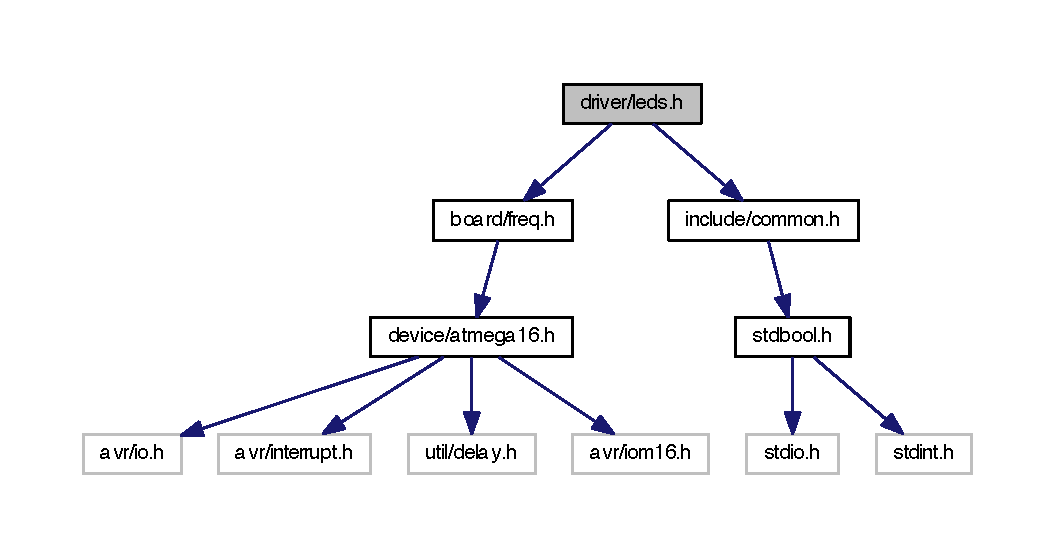
\includegraphics[width=350pt]{leds_8h__incl}
\end{center}
\end{figure}
This graph shows which files directly or indirectly include this file\+:
\nopagebreak
\begin{figure}[H]
\begin{center}
\leavevmode
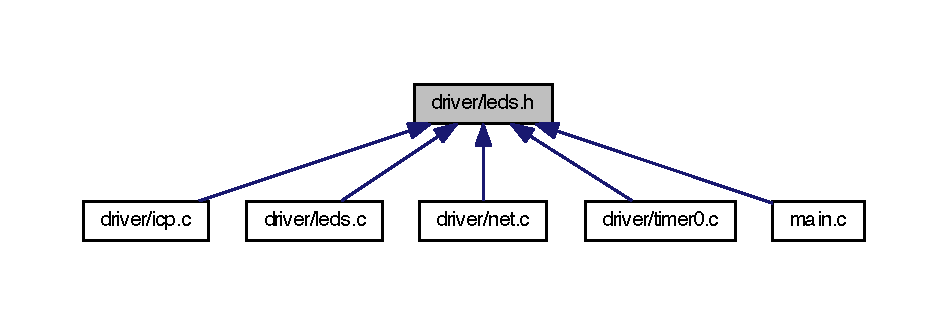
\includegraphics[width=350pt]{leds_8h__dep__incl}
\end{center}
\end{figure}
\subsection*{Functions}
\begin{DoxyCompactItemize}
\item 
void \hyperlink{leds_8h_a67cfc3137a465e560792490e81365254}{leds\+\_\+init} (void)
\begin{DoxyCompactList}\small\item\em initialize all L\+E\+Ds \end{DoxyCompactList}\item 
void \hyperlink{leds_8h_a6f9e25a266d32b9a09b420fcaf8696aa}{led\+\_\+init} (uint8\+\_\+t)
\begin{DoxyCompactList}\small\item\em initialize a led \end{DoxyCompactList}\item 
void \hyperlink{leds_8h_a4e79f1752d7b67cfed2c7831307cf32c}{leds\+\_\+on} (void)
\begin{DoxyCompactList}\small\item\em turn on all L\+E\+Ds \end{DoxyCompactList}\item 
void \hyperlink{leds_8h_af8d5030cf60431c05c249bcc2dc8b9c3}{led\+\_\+on} (uint8\+\_\+t)
\begin{DoxyCompactList}\small\item\em turn on a led \end{DoxyCompactList}\item 
void \hyperlink{leds_8h_a4bf53abfd4d628a2791bf1783de96b27}{leds\+\_\+off} (void)
\begin{DoxyCompactList}\small\item\em turn off all L\+E\+Ds \end{DoxyCompactList}\item 
void \hyperlink{leds_8h_aeb2c51827769b70ddb6a63692130c9fc}{led\+\_\+off} (uint8\+\_\+t)
\begin{DoxyCompactList}\small\item\em turn off a led \end{DoxyCompactList}\item 
void \hyperlink{leds_8h_a779f03508ef6685f03e64616c7c2fc58}{leds\+\_\+toggle} (void)
\begin{DoxyCompactList}\small\item\em toggle all L\+E\+Ds \end{DoxyCompactList}\item 
void \hyperlink{leds_8h_a5ab3085ed00fb0edf7180e9d6d8a2630}{led\+\_\+toggle} (uint8\+\_\+t)
\begin{DoxyCompactList}\small\item\em toggle a led \end{DoxyCompactList}\end{DoxyCompactItemize}


\subsection{Detailed Description}
specific header file for leds driver 

\begin{DoxyAuthor}{Author}
M. Ozgan, \href{mailto:mozgan@mozgan.org}{\tt mozgan@mozgan.\+org} 
\end{DoxyAuthor}
\begin{DoxyVersion}{Version}
1.\+0 
\end{DoxyVersion}
\begin{DoxyDate}{Date}
19.\+08.\+2013 15\+:28\+:53 
\end{DoxyDate}
\begin{DoxyParagraph}{Compiler}
gcc (on Mac, and 4.\+4\+B\+S\+D) 
\end{DoxyParagraph}
\begin{DoxyParagraph}{Company}
T\+U Wien 
\end{DoxyParagraph}


\begin{DoxyRefDesc}{Bug}
\item[\hyperlink{bug__bug000008}{Bug}]none \end{DoxyRefDesc}
\begin{DoxyRefDesc}{Todo}
\item[\hyperlink{todo__todo000008}{Todo}]none \end{DoxyRefDesc}


Definition in file \hyperlink{leds_8h_source}{leds.\+h}.



\subsection{Function Documentation}
\hypertarget{leds_8h_a6f9e25a266d32b9a09b420fcaf8696aa}{\index{leds.\+h@{leds.\+h}!led\+\_\+init@{led\+\_\+init}}
\index{led\+\_\+init@{led\+\_\+init}!leds.\+h@{leds.\+h}}
\subsubsection[{led\+\_\+init}]{\setlength{\rightskip}{0pt plus 5cm}void led\+\_\+init (
\begin{DoxyParamCaption}
\item[{uint8\+\_\+t}]{led}
\end{DoxyParamCaption}
)}}\label{leds_8h_a6f9e25a266d32b9a09b420fcaf8696aa}


initialize a led 


\begin{DoxyParams}{Parameters}
{\em led} & the number of led \\
\hline
\end{DoxyParams}


Definition at line 45 of file leds.\+c.



References L\+E\+D\+\_\+\+D\+D\+R, and L\+E\+D\+\_\+\+P\+O\+R\+T.

\hypertarget{leds_8h_aeb2c51827769b70ddb6a63692130c9fc}{\index{leds.\+h@{leds.\+h}!led\+\_\+off@{led\+\_\+off}}
\index{led\+\_\+off@{led\+\_\+off}!leds.\+h@{leds.\+h}}
\subsubsection[{led\+\_\+off}]{\setlength{\rightskip}{0pt plus 5cm}void led\+\_\+off (
\begin{DoxyParamCaption}
\item[{uint8\+\_\+t}]{led}
\end{DoxyParamCaption}
)}}\label{leds_8h_aeb2c51827769b70ddb6a63692130c9fc}


turn off a led 


\begin{DoxyParams}{Parameters}
{\em led} & the number of led \\
\hline
\end{DoxyParams}


Definition at line 86 of file leds.\+c.



References L\+E\+D\+\_\+\+P\+O\+R\+T.

\hypertarget{leds_8h_af8d5030cf60431c05c249bcc2dc8b9c3}{\index{leds.\+h@{leds.\+h}!led\+\_\+on@{led\+\_\+on}}
\index{led\+\_\+on@{led\+\_\+on}!leds.\+h@{leds.\+h}}
\subsubsection[{led\+\_\+on}]{\setlength{\rightskip}{0pt plus 5cm}void led\+\_\+on (
\begin{DoxyParamCaption}
\item[{uint8\+\_\+t}]{led}
\end{DoxyParamCaption}
)}}\label{leds_8h_af8d5030cf60431c05c249bcc2dc8b9c3}


turn on a led 


\begin{DoxyParams}{Parameters}
{\em led} & the number of led \\
\hline
\end{DoxyParams}


Definition at line 66 of file leds.\+c.



References L\+E\+D\+\_\+\+P\+O\+R\+T.

\hypertarget{leds_8h_a5ab3085ed00fb0edf7180e9d6d8a2630}{\index{leds.\+h@{leds.\+h}!led\+\_\+toggle@{led\+\_\+toggle}}
\index{led\+\_\+toggle@{led\+\_\+toggle}!leds.\+h@{leds.\+h}}
\subsubsection[{led\+\_\+toggle}]{\setlength{\rightskip}{0pt plus 5cm}void led\+\_\+toggle (
\begin{DoxyParamCaption}
\item[{uint8\+\_\+t}]{led}
\end{DoxyParamCaption}
)}}\label{leds_8h_a5ab3085ed00fb0edf7180e9d6d8a2630}


toggle a led 


\begin{DoxyParams}{Parameters}
{\em led} & the number of led \\
\hline
\end{DoxyParams}


Definition at line 106 of file leds.\+c.



References L\+E\+D\+\_\+\+P\+O\+R\+T.



Referenced by trigger().

\hypertarget{leds_8h_a67cfc3137a465e560792490e81365254}{\index{leds.\+h@{leds.\+h}!leds\+\_\+init@{leds\+\_\+init}}
\index{leds\+\_\+init@{leds\+\_\+init}!leds.\+h@{leds.\+h}}
\subsubsection[{leds\+\_\+init}]{\setlength{\rightskip}{0pt plus 5cm}void leds\+\_\+init (
\begin{DoxyParamCaption}
\item[{void}]{}
\end{DoxyParamCaption}
)}}\label{leds_8h_a67cfc3137a465e560792490e81365254}


initialize all L\+E\+Ds 



Definition at line 33 of file leds.\+c.



References L\+E\+D\+\_\+\+A\+L\+L, L\+E\+D\+\_\+\+D\+D\+R, L\+E\+D\+\_\+\+O\+F\+F, and L\+E\+D\+\_\+\+P\+O\+R\+T.



Referenced by main().

\hypertarget{leds_8h_a4bf53abfd4d628a2791bf1783de96b27}{\index{leds.\+h@{leds.\+h}!leds\+\_\+off@{leds\+\_\+off}}
\index{leds\+\_\+off@{leds\+\_\+off}!leds.\+h@{leds.\+h}}
\subsubsection[{leds\+\_\+off}]{\setlength{\rightskip}{0pt plus 5cm}void leds\+\_\+off (
\begin{DoxyParamCaption}
\item[{void}]{}
\end{DoxyParamCaption}
)}}\label{leds_8h_a4bf53abfd4d628a2791bf1783de96b27}


turn off all L\+E\+Ds 



Definition at line 75 of file leds.\+c.



References L\+E\+D\+\_\+\+O\+F\+F, and L\+E\+D\+\_\+\+P\+O\+R\+T.

\hypertarget{leds_8h_a4e79f1752d7b67cfed2c7831307cf32c}{\index{leds.\+h@{leds.\+h}!leds\+\_\+on@{leds\+\_\+on}}
\index{leds\+\_\+on@{leds\+\_\+on}!leds.\+h@{leds.\+h}}
\subsubsection[{leds\+\_\+on}]{\setlength{\rightskip}{0pt plus 5cm}void leds\+\_\+on (
\begin{DoxyParamCaption}
\item[{void}]{}
\end{DoxyParamCaption}
)}}\label{leds_8h_a4e79f1752d7b67cfed2c7831307cf32c}


turn on all L\+E\+Ds 



Definition at line 55 of file leds.\+c.



References L\+E\+D\+\_\+\+A\+L\+L, and L\+E\+D\+\_\+\+P\+O\+R\+T.

\hypertarget{leds_8h_a779f03508ef6685f03e64616c7c2fc58}{\index{leds.\+h@{leds.\+h}!leds\+\_\+toggle@{leds\+\_\+toggle}}
\index{leds\+\_\+toggle@{leds\+\_\+toggle}!leds.\+h@{leds.\+h}}
\subsubsection[{leds\+\_\+toggle}]{\setlength{\rightskip}{0pt plus 5cm}void leds\+\_\+toggle (
\begin{DoxyParamCaption}
\item[{void}]{}
\end{DoxyParamCaption}
)}}\label{leds_8h_a779f03508ef6685f03e64616c7c2fc58}


toggle all L\+E\+Ds 



Definition at line 95 of file leds.\+c.



References L\+E\+D\+\_\+\+A\+L\+L, and L\+E\+D\+\_\+\+P\+O\+R\+T.


\hypertarget{net_8c}{\section{driver/net.c File Reference}
\label{net_8c}\index{driver/net.\+c@{driver/net.\+c}}
}


driver for network communication  


{\ttfamily \#include $<$board/freq.\+h$>$}\\*
{\ttfamily \#include $<$device/enc28j60.\+h$>$}\\*
{\ttfamily \#include $<$driver/net.\+h$>$}\\*
{\ttfamily \#include $<$driver/leds.\+h$>$}\\*
Include dependency graph for net.\+c\+:
\nopagebreak
\begin{figure}[H]
\begin{center}
\leavevmode
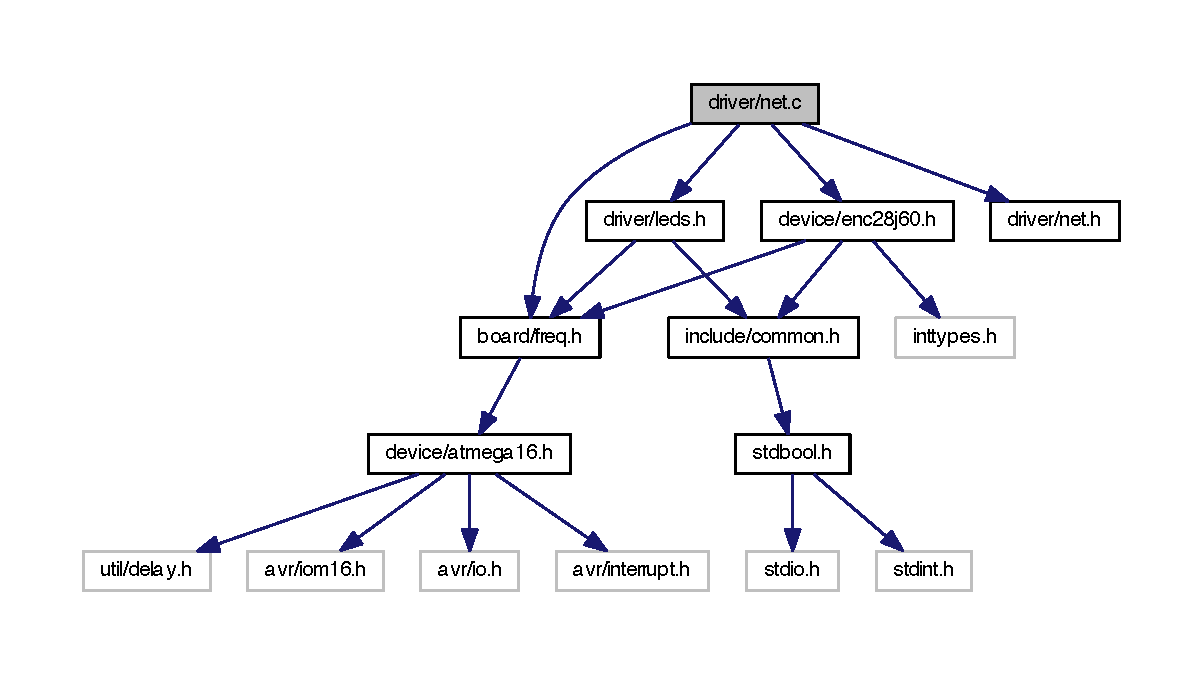
\includegraphics[width=350pt]{net_8c__incl}
\end{center}
\end{figure}
\subsection*{Functions}
\begin{DoxyCompactItemize}
\item 
void \hyperlink{net_8c_a044265f0081346e76e9686ec54badf5b}{net\+\_\+init} (uint8\+\_\+t $\ast$\hyperlink{main_8c_ae0177d7710b28f95720d54e2b1d37d65}{mymac}, uint8\+\_\+t $\ast$\hyperlink{main_8c_a60983d0ff040975723414a8f21375c77}{myip})
\begin{DoxyCompactList}\small\item\em initialize the network \end{DoxyCompactList}\item 
uint8\+\_\+t \hyperlink{net_8c_a2e5cb2f2e4db612d3ac1262da515f20f}{eth\+\_\+arp} (uint8\+\_\+t $\ast$\hyperlink{main_8c_aef549d19c508d258c21e95059b300d13}{buf}, uint8\+\_\+t len)
\begin{DoxyCompactList}\small\item\em make the network wirh arp \end{DoxyCompactList}\item 
uint8\+\_\+t \hyperlink{net_8c_af0b4a02ade3a716c6b10ce1fc821770b}{eth\+\_\+ip} (uint8\+\_\+t $\ast$\hyperlink{main_8c_aef549d19c508d258c21e95059b300d13}{buf}, uint8\+\_\+t len)
\begin{DoxyCompactList}\small\item\em make the network communication with ip address \end{DoxyCompactList}\item 
void \hyperlink{net_8c_ad8c59c931bff8fe806ce7598efb6047c}{arp\+\_\+answer} (uint8\+\_\+t $\ast$\hyperlink{main_8c_aef549d19c508d258c21e95059b300d13}{buf}, uint8\+\_\+t len)
\begin{DoxyCompactList}\small\item\em make an answer if request \end{DoxyCompactList}\item 
void \hyperlink{net_8c_a4f72e5a5ef17368554a9b5368d05b5bd}{echo\+\_\+reply} (uint8\+\_\+t $\ast$\hyperlink{main_8c_aef549d19c508d258c21e95059b300d13}{buf}, uint8\+\_\+t len)
\begin{DoxyCompactList}\small\item\em make an echo answer (ping -\/ pong) if request \end{DoxyCompactList}\item 
void \hyperlink{net_8c_a26c789f4ef67752529324ebba5ac51a1}{udp\+\_\+reply} (uint8\+\_\+t $\ast$\hyperlink{main_8c_aef549d19c508d258c21e95059b300d13}{buf}, char $\ast$data, uint8\+\_\+t len, uint16\+\_\+t port)
\begin{DoxyCompactList}\small\item\em make the U\+D\+P protocol \end{DoxyCompactList}\item 
void \hyperlink{net_8c_a0b1ae978a785d4da05a5c17be80f6314}{make\+\_\+eth} (uint8\+\_\+t $\ast$\hyperlink{main_8c_aef549d19c508d258c21e95059b300d13}{buf})
\begin{DoxyCompactList}\small\item\em make the ethernet header \end{DoxyCompactList}\item 
void \hyperlink{net_8c_a03c6b5196ad75d2eeca9ff69537a3214}{make\+\_\+ip} (uint8\+\_\+t $\ast$\hyperlink{main_8c_aef549d19c508d258c21e95059b300d13}{buf})
\begin{DoxyCompactList}\small\item\em make the ip header \end{DoxyCompactList}\item 
uint16\+\_\+t \hyperlink{net_8c_acda4291ff558e4c9c4ca87e87679e4a7}{checksum} (uint8\+\_\+t $\ast$\hyperlink{main_8c_aef549d19c508d258c21e95059b300d13}{buf}, uint16\+\_\+t len, uint8\+\_\+t type)
\begin{DoxyCompactList}\small\item\em checksum \end{DoxyCompactList}\end{DoxyCompactItemize}
\subsection*{Variables}
\begin{DoxyCompactItemize}
\item 
static uint8\+\_\+t \hyperlink{net_8c_ad6ffa7743848d35021d59a06df02d7cb}{macaddr} \mbox{[}6\mbox{]}
\item 
static uint8\+\_\+t \hyperlink{net_8c_a1c5949b1405b137e3beb728106cb127d}{ipaddr} \mbox{[}4\mbox{]}
\end{DoxyCompactItemize}


\subsection{Detailed Description}
driver for network communication 

\begin{DoxyAuthor}{Author}
M. Ozgan, \href{mailto:mozgan@mozgan.org}{\tt mozgan@mozgan.\+org} 
\end{DoxyAuthor}
\begin{DoxyVersion}{Version}
0.\+2 
\end{DoxyVersion}
\begin{DoxyDate}{Date}
20.\+08.\+2013 13\+:29\+:36 
\end{DoxyDate}
\begin{DoxyParagraph}{Compiler}
gcc (on Mac, G\+N\+U/\+Linux, 4.\+4\+B\+S\+D) 
\end{DoxyParagraph}
\begin{DoxyParagraph}{Company}
T\+U Wien 
\end{DoxyParagraph}


\begin{DoxyRefDesc}{Bug}
\item[\hyperlink{bug__bug000009}{Bug}]none \end{DoxyRefDesc}
\begin{DoxyRefDesc}{Todo}
\item[\hyperlink{todo__todo000009}{Todo}]none \end{DoxyRefDesc}


Definition in file \hyperlink{net_8c_source}{net.\+c}.



\subsection{Function Documentation}
\hypertarget{net_8c_ad8c59c931bff8fe806ce7598efb6047c}{\index{net.\+c@{net.\+c}!arp\+\_\+answer@{arp\+\_\+answer}}
\index{arp\+\_\+answer@{arp\+\_\+answer}!net.\+c@{net.\+c}}
\subsubsection[{arp\+\_\+answer}]{\setlength{\rightskip}{0pt plus 5cm}void arp\+\_\+answer (
\begin{DoxyParamCaption}
\item[{uint8\+\_\+t $\ast$}]{buf, }
\item[{uint8\+\_\+t}]{len}
\end{DoxyParamCaption}
)}}\label{net_8c_ad8c59c931bff8fe806ce7598efb6047c}


make an answer if request 


\begin{DoxyParams}{Parameters}
{\em buf} & buffer \\
\hline
{\em len} & length of buffer \\
\hline
\end{DoxyParams}


Definition at line 125 of file net.\+c.



References A\+R\+P\+\_\+\+D\+E\+S\+T\+\_\+\+I\+P\+\_\+\+P, A\+R\+P\+\_\+\+D\+E\+S\+T\+\_\+\+M\+A\+C\+\_\+\+P, A\+R\+P\+\_\+\+O\+P\+C\+O\+D\+E\+\_\+\+H\+\_\+\+P, A\+R\+P\+\_\+\+O\+P\+C\+O\+D\+E\+\_\+\+L\+\_\+\+P, A\+R\+P\+\_\+\+O\+P\+C\+O\+D\+E\+\_\+\+R\+E\+P\+L\+Y\+\_\+\+H\+\_\+\+V, A\+R\+P\+\_\+\+O\+P\+C\+O\+D\+E\+\_\+\+R\+E\+P\+L\+Y\+\_\+\+L\+\_\+\+V, A\+R\+P\+\_\+\+S\+R\+C\+\_\+\+I\+P\+\_\+\+P, A\+R\+P\+\_\+\+S\+R\+C\+\_\+\+M\+A\+C\+\_\+\+P, enc\+\_\+send\+\_\+packet(), ipaddr, macaddr, and make\+\_\+eth().



Referenced by main().



Here is the call graph for this function\+:
\nopagebreak
\begin{figure}[H]
\begin{center}
\leavevmode
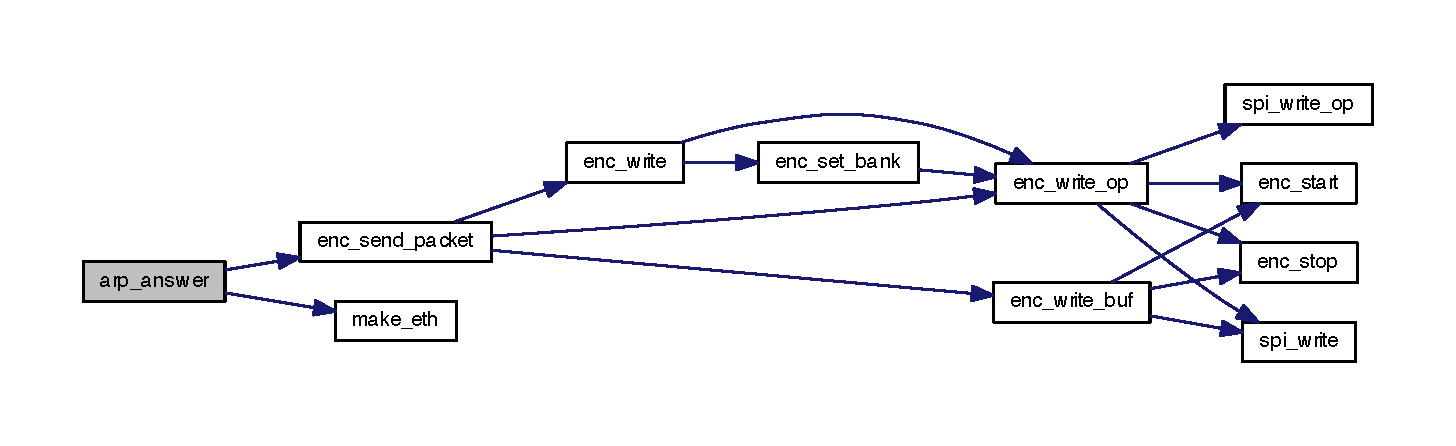
\includegraphics[width=350pt]{net_8c_ad8c59c931bff8fe806ce7598efb6047c_cgraph}
\end{center}
\end{figure}


\hypertarget{net_8c_acda4291ff558e4c9c4ca87e87679e4a7}{\index{net.\+c@{net.\+c}!checksum@{checksum}}
\index{checksum@{checksum}!net.\+c@{net.\+c}}
\subsubsection[{checksum}]{\setlength{\rightskip}{0pt plus 5cm}uint16\+\_\+t checksum (
\begin{DoxyParamCaption}
\item[{uint8\+\_\+t $\ast$}]{buf, }
\item[{uint16\+\_\+t}]{len, }
\item[{uint8\+\_\+t}]{type}
\end{DoxyParamCaption}
)}}\label{net_8c_acda4291ff558e4c9c4ca87e87679e4a7}


checksum 


\begin{DoxyParams}{Parameters}
{\em buf} & buffer \\
\hline
{\em len} & length \\
\hline
{\em type} & type\\
\hline
\end{DoxyParams}
\begin{DoxyReturn}{Returns}
sum 
\end{DoxyReturn}


Definition at line 277 of file net.\+c.



References buf, I\+P\+\_\+\+P\+R\+O\+T\+O\+\_\+\+T\+C\+P\+\_\+\+V, and I\+P\+\_\+\+P\+R\+O\+T\+O\+\_\+\+U\+D\+P\+\_\+\+V.



Referenced by make\+\_\+ip(), and udp\+\_\+reply().

\hypertarget{net_8c_a4f72e5a5ef17368554a9b5368d05b5bd}{\index{net.\+c@{net.\+c}!echo\+\_\+reply@{echo\+\_\+reply}}
\index{echo\+\_\+reply@{echo\+\_\+reply}!net.\+c@{net.\+c}}
\subsubsection[{echo\+\_\+reply}]{\setlength{\rightskip}{0pt plus 5cm}void echo\+\_\+reply (
\begin{DoxyParamCaption}
\item[{uint8\+\_\+t $\ast$}]{buf, }
\item[{uint8\+\_\+t}]{len}
\end{DoxyParamCaption}
)}}\label{net_8c_a4f72e5a5ef17368554a9b5368d05b5bd}


make an echo answer (ping -\/ pong) if request 


\begin{DoxyParams}{Parameters}
{\em buf} & buffer \\
\hline
{\em len} & length of buffer \\
\hline
\end{DoxyParams}


Definition at line 158 of file net.\+c.



References enc\+\_\+send\+\_\+packet(), I\+C\+M\+P\+\_\+\+C\+H\+E\+C\+K\+S\+U\+M\+\_\+\+P, I\+C\+M\+P\+\_\+\+R\+E\+P\+L\+Y\+\_\+\+V, I\+C\+M\+P\+\_\+\+T\+Y\+P\+E\+\_\+\+P, make\+\_\+eth(), and make\+\_\+ip().



Referenced by main().



Here is the call graph for this function\+:
\nopagebreak
\begin{figure}[H]
\begin{center}
\leavevmode
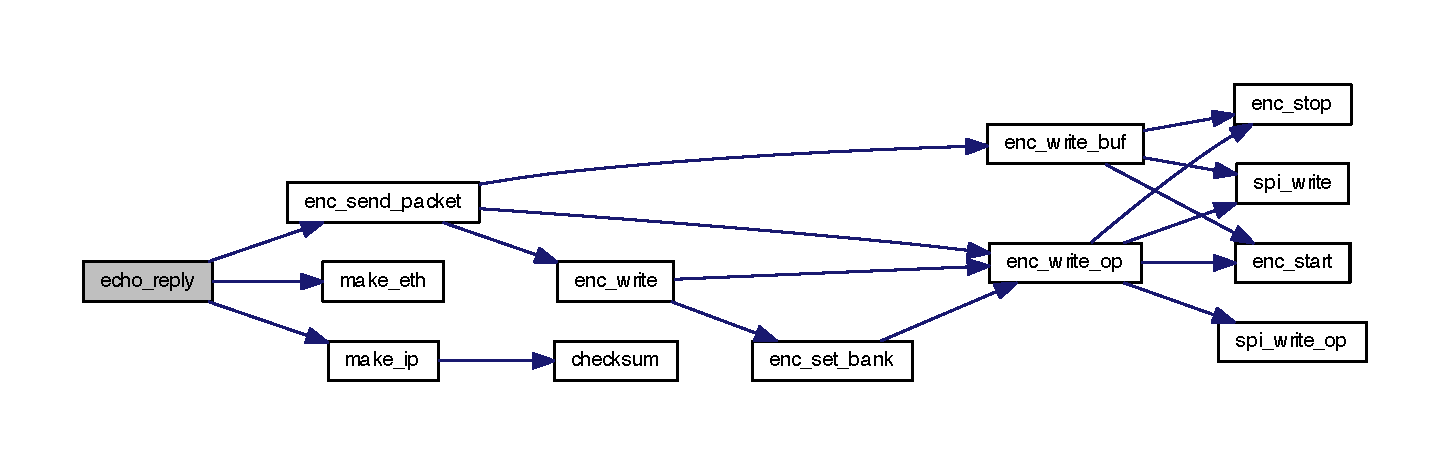
\includegraphics[width=350pt]{net_8c_a4f72e5a5ef17368554a9b5368d05b5bd_cgraph}
\end{center}
\end{figure}


\hypertarget{net_8c_a2e5cb2f2e4db612d3ac1262da515f20f}{\index{net.\+c@{net.\+c}!eth\+\_\+arp@{eth\+\_\+arp}}
\index{eth\+\_\+arp@{eth\+\_\+arp}!net.\+c@{net.\+c}}
\subsubsection[{eth\+\_\+arp}]{\setlength{\rightskip}{0pt plus 5cm}uint8\+\_\+t eth\+\_\+arp (
\begin{DoxyParamCaption}
\item[{uint8\+\_\+t $\ast$}]{buf, }
\item[{uint8\+\_\+t}]{len}
\end{DoxyParamCaption}
)}}\label{net_8c_a2e5cb2f2e4db612d3ac1262da515f20f}


make the network wirh arp 


\begin{DoxyParams}{Parameters}
{\em buf} & buffer \\
\hline
{\em len} & length of buffer\\
\hline
\end{DoxyParams}
\begin{DoxyReturn}{Returns}
return 1 if success, otherwise zero 
\end{DoxyReturn}


Definition at line 67 of file net.\+c.



References A\+R\+P\+\_\+\+D\+E\+S\+T\+\_\+\+I\+P\+\_\+\+P, E\+T\+H\+\_\+\+T\+Y\+P\+E\+\_\+\+H\+\_\+\+P, E\+T\+H\+\_\+\+T\+Y\+P\+E\+\_\+\+L\+\_\+\+P, E\+T\+H\+T\+Y\+P\+E\+\_\+\+A\+R\+P\+\_\+\+H\+\_\+\+V, E\+T\+H\+T\+Y\+P\+E\+\_\+\+A\+R\+P\+\_\+\+L\+\_\+\+V, and ipaddr.



Referenced by main().

\hypertarget{net_8c_af0b4a02ade3a716c6b10ce1fc821770b}{\index{net.\+c@{net.\+c}!eth\+\_\+ip@{eth\+\_\+ip}}
\index{eth\+\_\+ip@{eth\+\_\+ip}!net.\+c@{net.\+c}}
\subsubsection[{eth\+\_\+ip}]{\setlength{\rightskip}{0pt plus 5cm}uint8\+\_\+t eth\+\_\+ip (
\begin{DoxyParamCaption}
\item[{uint8\+\_\+t $\ast$}]{buf, }
\item[{uint8\+\_\+t}]{len}
\end{DoxyParamCaption}
)}}\label{net_8c_af0b4a02ade3a716c6b10ce1fc821770b}


make the network communication with ip address 


\begin{DoxyParams}{Parameters}
{\em buf} & buffer \\
\hline
{\em len} & length of buffer\\
\hline
\end{DoxyParams}
\begin{DoxyReturn}{Returns}
returns 1 if success, otherwise zero 
\end{DoxyReturn}


Definition at line 97 of file net.\+c.



References E\+T\+H\+\_\+\+T\+Y\+P\+E\+\_\+\+H\+\_\+\+P, E\+T\+H\+\_\+\+T\+Y\+P\+E\+\_\+\+L\+\_\+\+P, E\+T\+H\+T\+Y\+P\+E\+\_\+\+I\+P\+\_\+\+H\+\_\+\+V, E\+T\+H\+T\+Y\+P\+E\+\_\+\+I\+P\+\_\+\+L\+\_\+\+V, I\+P\+\_\+\+D\+E\+S\+T\+\_\+\+P, and ipaddr.



Referenced by main().

\hypertarget{net_8c_a0b1ae978a785d4da05a5c17be80f6314}{\index{net.\+c@{net.\+c}!make\+\_\+eth@{make\+\_\+eth}}
\index{make\+\_\+eth@{make\+\_\+eth}!net.\+c@{net.\+c}}
\subsubsection[{make\+\_\+eth}]{\setlength{\rightskip}{0pt plus 5cm}void make\+\_\+eth (
\begin{DoxyParamCaption}
\item[{uint8\+\_\+t $\ast$}]{buf}
\end{DoxyParamCaption}
)}}\label{net_8c_a0b1ae978a785d4da05a5c17be80f6314}


make the ethernet header 


\begin{DoxyParams}{Parameters}
{\em buf} & buffer \\
\hline
\end{DoxyParams}


Definition at line 225 of file net.\+c.



References E\+T\+H\+\_\+\+D\+E\+S\+T\+\_\+\+M\+A\+C, E\+T\+H\+\_\+\+S\+R\+C\+\_\+\+M\+A\+C, and macaddr.



Referenced by arp\+\_\+answer(), echo\+\_\+reply(), and udp\+\_\+reply().

\hypertarget{net_8c_a03c6b5196ad75d2eeca9ff69537a3214}{\index{net.\+c@{net.\+c}!make\+\_\+ip@{make\+\_\+ip}}
\index{make\+\_\+ip@{make\+\_\+ip}!net.\+c@{net.\+c}}
\subsubsection[{make\+\_\+ip}]{\setlength{\rightskip}{0pt plus 5cm}void make\+\_\+ip (
\begin{DoxyParamCaption}
\item[{uint8\+\_\+t $\ast$}]{buf}
\end{DoxyParamCaption}
)}}\label{net_8c_a03c6b5196ad75d2eeca9ff69537a3214}


make the ip header 


\begin{DoxyParams}{Parameters}
{\em buf} & \\
\hline
\end{DoxyParams}


Definition at line 242 of file net.\+c.



References checksum(), I\+P\+\_\+\+C\+H\+E\+C\+K\+S\+U\+M\+\_\+\+P, I\+P\+\_\+\+D\+E\+S\+T\+\_\+\+P, I\+P\+\_\+\+F\+L\+A\+G\+S\+\_\+\+P, I\+P\+\_\+\+H\+E\+A\+D\+E\+R\+\_\+\+L\+E\+N, I\+P\+\_\+\+P, I\+P\+\_\+\+S\+R\+C\+\_\+\+P, I\+P\+\_\+\+T\+T\+L\+\_\+\+P, and ipaddr.



Referenced by echo\+\_\+reply(), and udp\+\_\+reply().



Here is the call graph for this function\+:
\nopagebreak
\begin{figure}[H]
\begin{center}
\leavevmode
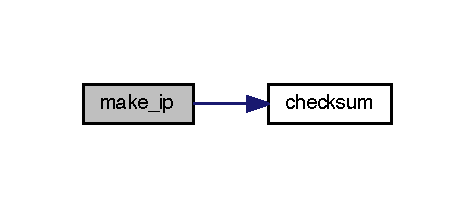
\includegraphics[width=228pt]{net_8c_a03c6b5196ad75d2eeca9ff69537a3214_cgraph}
\end{center}
\end{figure}


\hypertarget{net_8c_a044265f0081346e76e9686ec54badf5b}{\index{net.\+c@{net.\+c}!net\+\_\+init@{net\+\_\+init}}
\index{net\+\_\+init@{net\+\_\+init}!net.\+c@{net.\+c}}
\subsubsection[{net\+\_\+init}]{\setlength{\rightskip}{0pt plus 5cm}void net\+\_\+init (
\begin{DoxyParamCaption}
\item[{uint8\+\_\+t $\ast$}]{mymac, }
\item[{uint8\+\_\+t $\ast$}]{myip}
\end{DoxyParamCaption}
)}}\label{net_8c_a044265f0081346e76e9686ec54badf5b}


initialize the network 


\begin{DoxyParams}{Parameters}
{\em mymac} & my mac address \\
\hline
{\em myip} & my ip address \\
\hline
\end{DoxyParams}


Definition at line 43 of file net.\+c.



References ipaddr, and macaddr.



Referenced by main().

\hypertarget{net_8c_a26c789f4ef67752529324ebba5ac51a1}{\index{net.\+c@{net.\+c}!udp\+\_\+reply@{udp\+\_\+reply}}
\index{udp\+\_\+reply@{udp\+\_\+reply}!net.\+c@{net.\+c}}
\subsubsection[{udp\+\_\+reply}]{\setlength{\rightskip}{0pt plus 5cm}void udp\+\_\+reply (
\begin{DoxyParamCaption}
\item[{uint8\+\_\+t $\ast$}]{buf, }
\item[{char $\ast$}]{data, }
\item[{uint8\+\_\+t}]{len, }
\item[{uint16\+\_\+t}]{port}
\end{DoxyParamCaption}
)}}\label{net_8c_a26c789f4ef67752529324ebba5ac51a1}


make the U\+D\+P protocol 


\begin{DoxyParams}{Parameters}
{\em buf} & buffer \\
\hline
{\em data} & data \\
\hline
{\em len} & length \\
\hline
{\em port} & port number \\
\hline
\end{DoxyParams}


Definition at line 182 of file net.\+c.



References checksum(), enc\+\_\+send\+\_\+packet(), E\+T\+H\+\_\+\+H\+E\+A\+D\+E\+R\+\_\+\+L\+E\+N, I\+P\+\_\+\+H\+E\+A\+D\+E\+R\+\_\+\+L\+E\+N, I\+P\+\_\+\+S\+R\+C\+\_\+\+P, I\+P\+\_\+\+T\+O\+T\+L\+E\+N\+\_\+\+H\+\_\+\+P, I\+P\+\_\+\+T\+O\+T\+L\+E\+N\+\_\+\+L\+\_\+\+P, make\+\_\+eth(), make\+\_\+ip(), U\+D\+P\+\_\+\+C\+H\+E\+C\+K\+S\+U\+M\+\_\+\+H\+\_\+\+P, U\+D\+P\+\_\+\+C\+H\+E\+C\+K\+S\+U\+M\+\_\+\+L\+\_\+\+P, U\+D\+P\+\_\+\+D\+A\+T\+A\+\_\+\+P, U\+D\+P\+\_\+\+D\+E\+S\+T\+\_\+\+P\+O\+R\+T\+\_\+\+H\+\_\+\+P, U\+D\+P\+\_\+\+D\+E\+S\+T\+\_\+\+P\+O\+R\+T\+\_\+\+L\+\_\+\+P, U\+D\+P\+\_\+\+H\+E\+A\+D\+E\+R\+\_\+\+L\+E\+N, U\+D\+P\+\_\+\+L\+E\+N\+\_\+\+H\+\_\+\+P, U\+D\+P\+\_\+\+L\+E\+N\+\_\+\+L\+\_\+\+P, U\+D\+P\+\_\+\+S\+R\+C\+\_\+\+P\+O\+R\+T\+\_\+\+H\+\_\+\+P, and U\+D\+P\+\_\+\+S\+R\+C\+\_\+\+P\+O\+R\+T\+\_\+\+L\+\_\+\+P.



Referenced by main().



Here is the call graph for this function\+:
\nopagebreak
\begin{figure}[H]
\begin{center}
\leavevmode
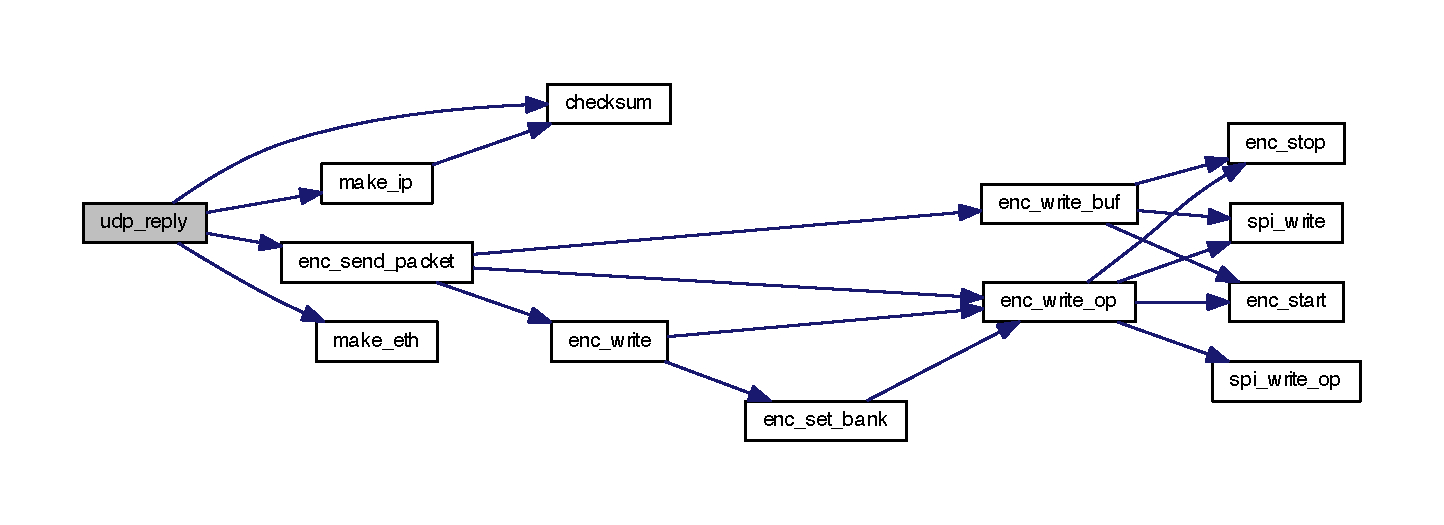
\includegraphics[width=350pt]{net_8c_a26c789f4ef67752529324ebba5ac51a1_cgraph}
\end{center}
\end{figure}




\subsection{Variable Documentation}
\hypertarget{net_8c_a1c5949b1405b137e3beb728106cb127d}{\index{net.\+c@{net.\+c}!ipaddr@{ipaddr}}
\index{ipaddr@{ipaddr}!net.\+c@{net.\+c}}
\subsubsection[{ipaddr}]{\setlength{\rightskip}{0pt plus 5cm}uint8\+\_\+t ipaddr\mbox{[}4\mbox{]}\hspace{0.3cm}{\ttfamily [static]}}}\label{net_8c_a1c5949b1405b137e3beb728106cb127d}


Definition at line 34 of file net.\+c.



Referenced by arp\+\_\+answer(), eth\+\_\+arp(), eth\+\_\+ip(), make\+\_\+ip(), and net\+\_\+init().

\hypertarget{net_8c_ad6ffa7743848d35021d59a06df02d7cb}{\index{net.\+c@{net.\+c}!macaddr@{macaddr}}
\index{macaddr@{macaddr}!net.\+c@{net.\+c}}
\subsubsection[{macaddr}]{\setlength{\rightskip}{0pt plus 5cm}uint8\+\_\+t macaddr\mbox{[}6\mbox{]}\hspace{0.3cm}{\ttfamily [static]}}}\label{net_8c_ad6ffa7743848d35021d59a06df02d7cb}


Definition at line 33 of file net.\+c.



Referenced by arp\+\_\+answer(), make\+\_\+eth(), and net\+\_\+init().


\hypertarget{net_8h}{\section{driver/net.h File Reference}
\label{net_8h}\index{driver/net.\+h@{driver/net.\+h}}
}


header file for network communication  


This graph shows which files directly or indirectly include this file\+:
\nopagebreak
\begin{figure}[H]
\begin{center}
\leavevmode
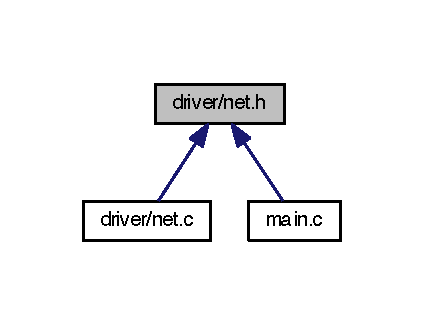
\includegraphics[width=204pt]{net_8h__dep__incl}
\end{center}
\end{figure}
\subsection*{Macros}
\begin{DoxyCompactItemize}
\item 
\#define \hyperlink{net_8h_a055d3f576495c1e6018012e1d952da1f}{E\+T\+H\+\_\+\+H\+E\+A\+D\+E\+R\+\_\+\+L\+E\+N}~14
\item 
\#define \hyperlink{net_8h_abe5d0b955430ac312d3b2fd96a5f67b5}{E\+T\+H\+T\+Y\+P\+E\+\_\+\+A\+R\+P\+\_\+\+H\+\_\+\+V}~0x08
\item 
\#define \hyperlink{net_8h_a77f5c72342c7d1813f76ee28382c9fa7}{E\+T\+H\+T\+Y\+P\+E\+\_\+\+A\+R\+P\+\_\+\+L\+\_\+\+V}~0x06
\item 
\#define \hyperlink{net_8h_abd570c69c474bff5874030a29ce83e80}{E\+T\+H\+T\+Y\+P\+E\+\_\+\+I\+P\+\_\+\+H\+\_\+\+V}~0x08
\item 
\#define \hyperlink{net_8h_a838baeea7a95a1fae5c01212d3ea699a}{E\+T\+H\+T\+Y\+P\+E\+\_\+\+I\+P\+\_\+\+L\+\_\+\+V}~0x00
\item 
\#define \hyperlink{net_8h_afa6d3ef1566c3290aab9916e63bf5fc5}{E\+T\+H\+\_\+\+T\+Y\+P\+E\+\_\+\+H\+\_\+\+P}~12
\item 
\#define \hyperlink{net_8h_a27cff6edf78472708f78ad7a90ef4be8}{E\+T\+H\+\_\+\+T\+Y\+P\+E\+\_\+\+L\+\_\+\+P}~13
\item 
\#define \hyperlink{net_8h_a9cff666f2a46f9b6e2bf5fccb3cd4bf5}{E\+T\+H\+\_\+\+D\+E\+S\+T\+\_\+\+M\+A\+C}~0
\item 
\#define \hyperlink{net_8h_a08c7f7257dfd57b273f26a044c83583a}{E\+T\+H\+\_\+\+S\+R\+C\+\_\+\+M\+A\+C}~6
\item 
\#define \hyperlink{net_8h_af5150574d180879e1aaddf354efbb8d8}{A\+R\+P\+\_\+\+O\+P\+C\+O\+D\+E\+\_\+\+R\+E\+P\+L\+Y\+\_\+\+H\+\_\+\+V}~0x00
\item 
\#define \hyperlink{net_8h_aebb42d1fdd50fc05c6cfac1d9d9a921c}{A\+R\+P\+\_\+\+O\+P\+C\+O\+D\+E\+\_\+\+R\+E\+P\+L\+Y\+\_\+\+L\+\_\+\+V}~0x02
\item 
\#define \hyperlink{net_8h_ae214faf8b2134cf18ca9977f6f00ff27}{A\+R\+P\+\_\+\+L\+\_\+\+V}~0x06
\item 
\#define \hyperlink{net_8h_a24cb4d09ea3c57338f540e097d8e5c67}{A\+R\+P\+\_\+\+D\+E\+S\+T\+\_\+\+I\+P\+\_\+\+P}~0x26
\item 
\#define \hyperlink{net_8h_ab61b9675756588bd594b80ce642c2d3c}{A\+R\+P\+\_\+\+O\+P\+C\+O\+D\+E\+\_\+\+H\+\_\+\+P}~0x14
\item 
\#define \hyperlink{net_8h_a3549c08e735441fe5d6963dbc377fc22}{A\+R\+P\+\_\+\+O\+P\+C\+O\+D\+E\+\_\+\+L\+\_\+\+P}~0x15
\item 
\#define \hyperlink{net_8h_a9948fcfc68fa12b340c92f086bbecc6e}{A\+R\+P\+\_\+\+S\+R\+C\+\_\+\+M\+A\+C\+\_\+\+P}~0x16
\item 
\#define \hyperlink{net_8h_a5b1093f70c64545b8282c49b0c23c60e}{A\+R\+P\+\_\+\+S\+R\+C\+\_\+\+I\+P\+\_\+\+P}~0x1\+C
\item 
\#define \hyperlink{net_8h_ad001cbaeab73f9da78a29b6b03a89a78}{A\+R\+P\+\_\+\+D\+E\+S\+T\+\_\+\+M\+A\+C\+\_\+\+P}~0x20
\item 
\#define \hyperlink{net_8h_a24cb4d09ea3c57338f540e097d8e5c67}{A\+R\+P\+\_\+\+D\+E\+S\+T\+\_\+\+I\+P\+\_\+\+P}~0x26
\item 
\#define \hyperlink{net_8h_a956b187f1ee557ac6c330bc95bad53e9}{I\+P\+\_\+\+H\+E\+A\+D\+E\+R\+\_\+\+L\+E\+N}~20
\item 
\#define \hyperlink{net_8h_a9288e7acf3c9011f0f99eed5ea866698}{I\+P\+\_\+\+S\+R\+C\+\_\+\+P}~0x1\+A
\item 
\#define \hyperlink{net_8h_af8aa92ed67ae1b8c9e0ee96107b7f8cd}{I\+P\+\_\+\+D\+E\+S\+T\+\_\+\+P}~0x1\+E
\item 
\#define \hyperlink{net_8h_ad3e2eb9acb5d5e133af3ce68a3cd5b2a}{I\+P\+\_\+\+C\+H\+E\+C\+K\+S\+U\+M\+\_\+\+P}~0x18
\item 
\#define \hyperlink{net_8h_a5c6cdbd7479e284f33e2b291d40fe389}{I\+P\+\_\+\+T\+T\+L\+\_\+\+P}~0x16
\item 
\#define \hyperlink{net_8h_a1101d91e0c5eae35609dd0a3df5a196b}{I\+P\+\_\+\+F\+L\+A\+G\+S\+\_\+\+P}~0x14
\item 
\#define \hyperlink{net_8h_a971527e7fb194f5f15b6c7ffcfcc3916}{I\+P\+\_\+\+P}~0x0\+E
\item 
\#define \hyperlink{net_8h_a07afbd22b129e73427b7ff01463b24ea}{I\+P\+\_\+\+T\+O\+T\+L\+E\+N\+\_\+\+H\+\_\+\+P}~0x10
\item 
\#define \hyperlink{net_8h_a970d4973348f49ab866cabd98ebf06f8}{I\+P\+\_\+\+T\+O\+T\+L\+E\+N\+\_\+\+L\+\_\+\+P}~0x11
\item 
\#define \hyperlink{net_8h_a94a24147ac9e4282e3dc3109916eceee}{I\+P\+\_\+\+P\+R\+O\+T\+O\+\_\+\+P}~0x17
\item 
\#define \hyperlink{net_8h_a5ac4d574d1b2e5119c7ab8c2b74be434}{I\+P\+\_\+\+P\+R\+O\+T\+O\+\_\+\+I\+C\+M\+P\+\_\+\+V}~1
\item 
\#define \hyperlink{net_8h_a9c81cf21add56a1f1fb3d59df1d6a5c8}{I\+P\+\_\+\+P\+R\+O\+T\+O\+\_\+\+T\+C\+P\+\_\+\+V}~6
\item 
\#define \hyperlink{net_8h_af197bd006505ea01b4cafbf596916af7}{I\+P\+\_\+\+P\+R\+O\+T\+O\+\_\+\+U\+D\+P\+\_\+\+V}~17
\item 
\#define \hyperlink{net_8h_a8bf333ae8f88e31ca100f3eba691a67d}{I\+C\+M\+P\+\_\+\+R\+E\+P\+L\+Y\+\_\+\+V}~0
\item 
\#define \hyperlink{net_8h_a7759a689bdd28850817c7de8869d35c4}{I\+C\+M\+P\+\_\+\+R\+E\+Q\+U\+E\+S\+T\+\_\+\+V}~8
\item 
\#define \hyperlink{net_8h_af4d84ceabffe9baf6af2687d56657dfe}{I\+C\+M\+P\+\_\+\+T\+Y\+P\+E\+\_\+\+P}~0x22
\item 
\#define \hyperlink{net_8h_a2d857ee9bba69c4511b2acad46b23e49}{I\+C\+M\+P\+\_\+\+C\+H\+E\+C\+K\+S\+U\+M\+\_\+\+P}~0x24
\item 
\#define \hyperlink{net_8h_ac8932031ba2c6d324056a751296553ba}{U\+D\+P\+\_\+\+H\+E\+A\+D\+E\+R\+\_\+\+L\+E\+N}~8
\item 
\#define \hyperlink{net_8h_acc96829b7e154cccadc0e5211f16a803}{U\+D\+P\+\_\+\+S\+R\+C\+\_\+\+P\+O\+R\+T\+\_\+\+H\+\_\+\+P}~0x22
\item 
\#define \hyperlink{net_8h_abcb0833d59b139c4641ae397f2dd2067}{U\+D\+P\+\_\+\+S\+R\+C\+\_\+\+P\+O\+R\+T\+\_\+\+L\+\_\+\+P}~0x23
\item 
\#define \hyperlink{net_8h_afb844f54f480d81c927f6e619433f80d}{U\+D\+P\+\_\+\+D\+E\+S\+T\+\_\+\+P\+O\+R\+T\+\_\+\+H\+\_\+\+P}~0x24
\item 
\#define \hyperlink{net_8h_a1c49b298edc29ffd4770cf202d91f672}{U\+D\+P\+\_\+\+D\+E\+S\+T\+\_\+\+P\+O\+R\+T\+\_\+\+L\+\_\+\+P}~0x25
\item 
\#define \hyperlink{net_8h_ad09eed4965e5328be4c917e1ffd78e54}{U\+D\+P\+\_\+\+L\+E\+N\+\_\+\+H\+\_\+\+P}~0x26
\item 
\#define \hyperlink{net_8h_abce857433254bf3e2b5e5f1b65dc2e45}{U\+D\+P\+\_\+\+L\+E\+N\+\_\+\+L\+\_\+\+P}~0x27
\item 
\#define \hyperlink{net_8h_af823ef0dbb12f00f8bdcf6f8bb44cb96}{U\+D\+P\+\_\+\+C\+H\+E\+C\+K\+S\+U\+M\+\_\+\+H\+\_\+\+P}~0x28
\item 
\#define \hyperlink{net_8h_a56590a4e078c15a9992b81d0e4071950}{U\+D\+P\+\_\+\+C\+H\+E\+C\+K\+S\+U\+M\+\_\+\+L\+\_\+\+P}~0x29
\item 
\#define \hyperlink{net_8h_ac885920a5ba75634915351b35c577928}{U\+D\+P\+\_\+\+D\+A\+T\+A\+\_\+\+P}~0x2\+A
\end{DoxyCompactItemize}
\subsection*{Functions}
\begin{DoxyCompactItemize}
\item 
void \hyperlink{net_8h_ae66d6e0f4a7fee030d0b181873fd3c43}{net\+\_\+init} (uint8\+\_\+t $\ast$, uint8\+\_\+t $\ast$)
\begin{DoxyCompactList}\small\item\em initialize the network \end{DoxyCompactList}\item 
uint8\+\_\+t \hyperlink{net_8h_adad2aa706a7d44a4993c12aeeb0f3ee5}{eth\+\_\+arp} (uint8\+\_\+t $\ast$, uint8\+\_\+t)
\begin{DoxyCompactList}\small\item\em make the network wirh arp \end{DoxyCompactList}\item 
uint8\+\_\+t \hyperlink{net_8h_a29b7bf9dc451b96400620066cfd4122a}{eth\+\_\+ip} (uint8\+\_\+t $\ast$, uint8\+\_\+t)
\begin{DoxyCompactList}\small\item\em make the network communication with ip address \end{DoxyCompactList}\item 
void \hyperlink{net_8h_a28773a34ece2b6d44dd567c8b110a4d0}{arp\+\_\+answer} (uint8\+\_\+t $\ast$, uint8\+\_\+t)
\begin{DoxyCompactList}\small\item\em make an answer if request \end{DoxyCompactList}\item 
void \hyperlink{net_8h_a373984d10afb4fc42dca8b356b39d245}{echo\+\_\+reply} (uint8\+\_\+t $\ast$, uint8\+\_\+t)
\begin{DoxyCompactList}\small\item\em make an echo answer (ping -\/ pong) if request \end{DoxyCompactList}\item 
void \hyperlink{net_8h_ad6dd37c1e1e4f4a907f53c406a088cb3}{udp\+\_\+reply} (uint8\+\_\+t $\ast$, char $\ast$, uint8\+\_\+t, uint16\+\_\+t)
\begin{DoxyCompactList}\small\item\em make the U\+D\+P protocol \end{DoxyCompactList}\item 
void \hyperlink{net_8h_af8b6b03bdab2ed94c16fa6370cf806d6}{make\+\_\+eth} (uint8\+\_\+t $\ast$)
\begin{DoxyCompactList}\small\item\em make the ethernet header \end{DoxyCompactList}\item 
void \hyperlink{net_8h_a57c50aa78a3b5d2dc8d8fd21d7ced975}{make\+\_\+ip} (uint8\+\_\+t $\ast$)
\begin{DoxyCompactList}\small\item\em make the ip header \end{DoxyCompactList}\item 
uint16\+\_\+t \hyperlink{net_8h_ae7ef39d9ed2b416c9fa575806e63ecb6}{checksum} (uint8\+\_\+t $\ast$, uint16\+\_\+t, uint8\+\_\+t)
\begin{DoxyCompactList}\small\item\em checksum \end{DoxyCompactList}\end{DoxyCompactItemize}


\subsection{Detailed Description}
header file for network communication 

\begin{DoxyAuthor}{Author}
M. Ozgan, \href{mailto:mozgan@mozgan.org}{\tt mozgan@mozgan.\+org} 
\end{DoxyAuthor}
\begin{DoxyVersion}{Version}
0.\+2 
\end{DoxyVersion}
\begin{DoxyDate}{Date}
20.\+08.\+2013 13\+:27\+:19 
\end{DoxyDate}
\begin{DoxyParagraph}{Compiler}
gcc (on Mac, G\+N\+U/\+Linux and 4.\+4\+B\+S\+D) 
\end{DoxyParagraph}
\begin{DoxyParagraph}{Company}
T\+U Wien 
\end{DoxyParagraph}


\begin{DoxyRefDesc}{Bug}
\item[\hyperlink{bug__bug000010}{Bug}]none \end{DoxyRefDesc}
\begin{DoxyRefDesc}{Todo}
\item[\hyperlink{todo__todo000010}{Todo}]none \end{DoxyRefDesc}


Definition in file \hyperlink{net_8h_source}{net.\+h}.



\subsection{Macro Definition Documentation}
\hypertarget{net_8h_a24cb4d09ea3c57338f540e097d8e5c67}{\index{net.\+h@{net.\+h}!A\+R\+P\+\_\+\+D\+E\+S\+T\+\_\+\+I\+P\+\_\+\+P@{A\+R\+P\+\_\+\+D\+E\+S\+T\+\_\+\+I\+P\+\_\+\+P}}
\index{A\+R\+P\+\_\+\+D\+E\+S\+T\+\_\+\+I\+P\+\_\+\+P@{A\+R\+P\+\_\+\+D\+E\+S\+T\+\_\+\+I\+P\+\_\+\+P}!net.\+h@{net.\+h}}
\subsubsection[{A\+R\+P\+\_\+\+D\+E\+S\+T\+\_\+\+I\+P\+\_\+\+P}]{\setlength{\rightskip}{0pt plus 5cm}\#define A\+R\+P\+\_\+\+D\+E\+S\+T\+\_\+\+I\+P\+\_\+\+P~0x26}}\label{net_8h_a24cb4d09ea3c57338f540e097d8e5c67}


Definition at line 88 of file net.\+h.



Referenced by arp\+\_\+answer(), and eth\+\_\+arp().

\hypertarget{net_8h_a24cb4d09ea3c57338f540e097d8e5c67}{\index{net.\+h@{net.\+h}!A\+R\+P\+\_\+\+D\+E\+S\+T\+\_\+\+I\+P\+\_\+\+P@{A\+R\+P\+\_\+\+D\+E\+S\+T\+\_\+\+I\+P\+\_\+\+P}}
\index{A\+R\+P\+\_\+\+D\+E\+S\+T\+\_\+\+I\+P\+\_\+\+P@{A\+R\+P\+\_\+\+D\+E\+S\+T\+\_\+\+I\+P\+\_\+\+P}!net.\+h@{net.\+h}}
\subsubsection[{A\+R\+P\+\_\+\+D\+E\+S\+T\+\_\+\+I\+P\+\_\+\+P}]{\setlength{\rightskip}{0pt plus 5cm}\#define A\+R\+P\+\_\+\+D\+E\+S\+T\+\_\+\+I\+P\+\_\+\+P~0x26}}\label{net_8h_a24cb4d09ea3c57338f540e097d8e5c67}


Definition at line 88 of file net.\+h.

\hypertarget{net_8h_ad001cbaeab73f9da78a29b6b03a89a78}{\index{net.\+h@{net.\+h}!A\+R\+P\+\_\+\+D\+E\+S\+T\+\_\+\+M\+A\+C\+\_\+\+P@{A\+R\+P\+\_\+\+D\+E\+S\+T\+\_\+\+M\+A\+C\+\_\+\+P}}
\index{A\+R\+P\+\_\+\+D\+E\+S\+T\+\_\+\+M\+A\+C\+\_\+\+P@{A\+R\+P\+\_\+\+D\+E\+S\+T\+\_\+\+M\+A\+C\+\_\+\+P}!net.\+h@{net.\+h}}
\subsubsection[{A\+R\+P\+\_\+\+D\+E\+S\+T\+\_\+\+M\+A\+C\+\_\+\+P}]{\setlength{\rightskip}{0pt plus 5cm}\#define A\+R\+P\+\_\+\+D\+E\+S\+T\+\_\+\+M\+A\+C\+\_\+\+P~0x20}}\label{net_8h_ad001cbaeab73f9da78a29b6b03a89a78}


Definition at line 87 of file net.\+h.



Referenced by arp\+\_\+answer().

\hypertarget{net_8h_ae214faf8b2134cf18ca9977f6f00ff27}{\index{net.\+h@{net.\+h}!A\+R\+P\+\_\+\+L\+\_\+\+V@{A\+R\+P\+\_\+\+L\+\_\+\+V}}
\index{A\+R\+P\+\_\+\+L\+\_\+\+V@{A\+R\+P\+\_\+\+L\+\_\+\+V}!net.\+h@{net.\+h}}
\subsubsection[{A\+R\+P\+\_\+\+L\+\_\+\+V}]{\setlength{\rightskip}{0pt plus 5cm}\#define A\+R\+P\+\_\+\+L\+\_\+\+V~0x06}}\label{net_8h_ae214faf8b2134cf18ca9977f6f00ff27}


Definition at line 79 of file net.\+h.

\hypertarget{net_8h_ab61b9675756588bd594b80ce642c2d3c}{\index{net.\+h@{net.\+h}!A\+R\+P\+\_\+\+O\+P\+C\+O\+D\+E\+\_\+\+H\+\_\+\+P@{A\+R\+P\+\_\+\+O\+P\+C\+O\+D\+E\+\_\+\+H\+\_\+\+P}}
\index{A\+R\+P\+\_\+\+O\+P\+C\+O\+D\+E\+\_\+\+H\+\_\+\+P@{A\+R\+P\+\_\+\+O\+P\+C\+O\+D\+E\+\_\+\+H\+\_\+\+P}!net.\+h@{net.\+h}}
\subsubsection[{A\+R\+P\+\_\+\+O\+P\+C\+O\+D\+E\+\_\+\+H\+\_\+\+P}]{\setlength{\rightskip}{0pt plus 5cm}\#define A\+R\+P\+\_\+\+O\+P\+C\+O\+D\+E\+\_\+\+H\+\_\+\+P~0x14}}\label{net_8h_ab61b9675756588bd594b80ce642c2d3c}


Definition at line 82 of file net.\+h.



Referenced by arp\+\_\+answer().

\hypertarget{net_8h_a3549c08e735441fe5d6963dbc377fc22}{\index{net.\+h@{net.\+h}!A\+R\+P\+\_\+\+O\+P\+C\+O\+D\+E\+\_\+\+L\+\_\+\+P@{A\+R\+P\+\_\+\+O\+P\+C\+O\+D\+E\+\_\+\+L\+\_\+\+P}}
\index{A\+R\+P\+\_\+\+O\+P\+C\+O\+D\+E\+\_\+\+L\+\_\+\+P@{A\+R\+P\+\_\+\+O\+P\+C\+O\+D\+E\+\_\+\+L\+\_\+\+P}!net.\+h@{net.\+h}}
\subsubsection[{A\+R\+P\+\_\+\+O\+P\+C\+O\+D\+E\+\_\+\+L\+\_\+\+P}]{\setlength{\rightskip}{0pt plus 5cm}\#define A\+R\+P\+\_\+\+O\+P\+C\+O\+D\+E\+\_\+\+L\+\_\+\+P~0x15}}\label{net_8h_a3549c08e735441fe5d6963dbc377fc22}


Definition at line 83 of file net.\+h.



Referenced by arp\+\_\+answer().

\hypertarget{net_8h_af5150574d180879e1aaddf354efbb8d8}{\index{net.\+h@{net.\+h}!A\+R\+P\+\_\+\+O\+P\+C\+O\+D\+E\+\_\+\+R\+E\+P\+L\+Y\+\_\+\+H\+\_\+\+V@{A\+R\+P\+\_\+\+O\+P\+C\+O\+D\+E\+\_\+\+R\+E\+P\+L\+Y\+\_\+\+H\+\_\+\+V}}
\index{A\+R\+P\+\_\+\+O\+P\+C\+O\+D\+E\+\_\+\+R\+E\+P\+L\+Y\+\_\+\+H\+\_\+\+V@{A\+R\+P\+\_\+\+O\+P\+C\+O\+D\+E\+\_\+\+R\+E\+P\+L\+Y\+\_\+\+H\+\_\+\+V}!net.\+h@{net.\+h}}
\subsubsection[{A\+R\+P\+\_\+\+O\+P\+C\+O\+D\+E\+\_\+\+R\+E\+P\+L\+Y\+\_\+\+H\+\_\+\+V}]{\setlength{\rightskip}{0pt plus 5cm}\#define A\+R\+P\+\_\+\+O\+P\+C\+O\+D\+E\+\_\+\+R\+E\+P\+L\+Y\+\_\+\+H\+\_\+\+V~0x00}}\label{net_8h_af5150574d180879e1aaddf354efbb8d8}


Definition at line 76 of file net.\+h.



Referenced by arp\+\_\+answer().

\hypertarget{net_8h_aebb42d1fdd50fc05c6cfac1d9d9a921c}{\index{net.\+h@{net.\+h}!A\+R\+P\+\_\+\+O\+P\+C\+O\+D\+E\+\_\+\+R\+E\+P\+L\+Y\+\_\+\+L\+\_\+\+V@{A\+R\+P\+\_\+\+O\+P\+C\+O\+D\+E\+\_\+\+R\+E\+P\+L\+Y\+\_\+\+L\+\_\+\+V}}
\index{A\+R\+P\+\_\+\+O\+P\+C\+O\+D\+E\+\_\+\+R\+E\+P\+L\+Y\+\_\+\+L\+\_\+\+V@{A\+R\+P\+\_\+\+O\+P\+C\+O\+D\+E\+\_\+\+R\+E\+P\+L\+Y\+\_\+\+L\+\_\+\+V}!net.\+h@{net.\+h}}
\subsubsection[{A\+R\+P\+\_\+\+O\+P\+C\+O\+D\+E\+\_\+\+R\+E\+P\+L\+Y\+\_\+\+L\+\_\+\+V}]{\setlength{\rightskip}{0pt plus 5cm}\#define A\+R\+P\+\_\+\+O\+P\+C\+O\+D\+E\+\_\+\+R\+E\+P\+L\+Y\+\_\+\+L\+\_\+\+V~0x02}}\label{net_8h_aebb42d1fdd50fc05c6cfac1d9d9a921c}


Definition at line 77 of file net.\+h.



Referenced by arp\+\_\+answer().

\hypertarget{net_8h_a5b1093f70c64545b8282c49b0c23c60e}{\index{net.\+h@{net.\+h}!A\+R\+P\+\_\+\+S\+R\+C\+\_\+\+I\+P\+\_\+\+P@{A\+R\+P\+\_\+\+S\+R\+C\+\_\+\+I\+P\+\_\+\+P}}
\index{A\+R\+P\+\_\+\+S\+R\+C\+\_\+\+I\+P\+\_\+\+P@{A\+R\+P\+\_\+\+S\+R\+C\+\_\+\+I\+P\+\_\+\+P}!net.\+h@{net.\+h}}
\subsubsection[{A\+R\+P\+\_\+\+S\+R\+C\+\_\+\+I\+P\+\_\+\+P}]{\setlength{\rightskip}{0pt plus 5cm}\#define A\+R\+P\+\_\+\+S\+R\+C\+\_\+\+I\+P\+\_\+\+P~0x1\+C}}\label{net_8h_a5b1093f70c64545b8282c49b0c23c60e}


Definition at line 86 of file net.\+h.



Referenced by arp\+\_\+answer().

\hypertarget{net_8h_a9948fcfc68fa12b340c92f086bbecc6e}{\index{net.\+h@{net.\+h}!A\+R\+P\+\_\+\+S\+R\+C\+\_\+\+M\+A\+C\+\_\+\+P@{A\+R\+P\+\_\+\+S\+R\+C\+\_\+\+M\+A\+C\+\_\+\+P}}
\index{A\+R\+P\+\_\+\+S\+R\+C\+\_\+\+M\+A\+C\+\_\+\+P@{A\+R\+P\+\_\+\+S\+R\+C\+\_\+\+M\+A\+C\+\_\+\+P}!net.\+h@{net.\+h}}
\subsubsection[{A\+R\+P\+\_\+\+S\+R\+C\+\_\+\+M\+A\+C\+\_\+\+P}]{\setlength{\rightskip}{0pt plus 5cm}\#define A\+R\+P\+\_\+\+S\+R\+C\+\_\+\+M\+A\+C\+\_\+\+P~0x16}}\label{net_8h_a9948fcfc68fa12b340c92f086bbecc6e}


Definition at line 85 of file net.\+h.



Referenced by arp\+\_\+answer().

\hypertarget{net_8h_a9cff666f2a46f9b6e2bf5fccb3cd4bf5}{\index{net.\+h@{net.\+h}!E\+T\+H\+\_\+\+D\+E\+S\+T\+\_\+\+M\+A\+C@{E\+T\+H\+\_\+\+D\+E\+S\+T\+\_\+\+M\+A\+C}}
\index{E\+T\+H\+\_\+\+D\+E\+S\+T\+\_\+\+M\+A\+C@{E\+T\+H\+\_\+\+D\+E\+S\+T\+\_\+\+M\+A\+C}!net.\+h@{net.\+h}}
\subsubsection[{E\+T\+H\+\_\+\+D\+E\+S\+T\+\_\+\+M\+A\+C}]{\setlength{\rightskip}{0pt plus 5cm}\#define E\+T\+H\+\_\+\+D\+E\+S\+T\+\_\+\+M\+A\+C~0}}\label{net_8h_a9cff666f2a46f9b6e2bf5fccb3cd4bf5}


Definition at line 72 of file net.\+h.



Referenced by make\+\_\+eth().

\hypertarget{net_8h_a055d3f576495c1e6018012e1d952da1f}{\index{net.\+h@{net.\+h}!E\+T\+H\+\_\+\+H\+E\+A\+D\+E\+R\+\_\+\+L\+E\+N@{E\+T\+H\+\_\+\+H\+E\+A\+D\+E\+R\+\_\+\+L\+E\+N}}
\index{E\+T\+H\+\_\+\+H\+E\+A\+D\+E\+R\+\_\+\+L\+E\+N@{E\+T\+H\+\_\+\+H\+E\+A\+D\+E\+R\+\_\+\+L\+E\+N}!net.\+h@{net.\+h}}
\subsubsection[{E\+T\+H\+\_\+\+H\+E\+A\+D\+E\+R\+\_\+\+L\+E\+N}]{\setlength{\rightskip}{0pt plus 5cm}\#define E\+T\+H\+\_\+\+H\+E\+A\+D\+E\+R\+\_\+\+L\+E\+N~14}}\label{net_8h_a055d3f576495c1e6018012e1d952da1f}


Definition at line 61 of file net.\+h.



Referenced by udp\+\_\+reply().

\hypertarget{net_8h_a08c7f7257dfd57b273f26a044c83583a}{\index{net.\+h@{net.\+h}!E\+T\+H\+\_\+\+S\+R\+C\+\_\+\+M\+A\+C@{E\+T\+H\+\_\+\+S\+R\+C\+\_\+\+M\+A\+C}}
\index{E\+T\+H\+\_\+\+S\+R\+C\+\_\+\+M\+A\+C@{E\+T\+H\+\_\+\+S\+R\+C\+\_\+\+M\+A\+C}!net.\+h@{net.\+h}}
\subsubsection[{E\+T\+H\+\_\+\+S\+R\+C\+\_\+\+M\+A\+C}]{\setlength{\rightskip}{0pt plus 5cm}\#define E\+T\+H\+\_\+\+S\+R\+C\+\_\+\+M\+A\+C~6}}\label{net_8h_a08c7f7257dfd57b273f26a044c83583a}


Definition at line 73 of file net.\+h.



Referenced by make\+\_\+eth().

\hypertarget{net_8h_afa6d3ef1566c3290aab9916e63bf5fc5}{\index{net.\+h@{net.\+h}!E\+T\+H\+\_\+\+T\+Y\+P\+E\+\_\+\+H\+\_\+\+P@{E\+T\+H\+\_\+\+T\+Y\+P\+E\+\_\+\+H\+\_\+\+P}}
\index{E\+T\+H\+\_\+\+T\+Y\+P\+E\+\_\+\+H\+\_\+\+P@{E\+T\+H\+\_\+\+T\+Y\+P\+E\+\_\+\+H\+\_\+\+P}!net.\+h@{net.\+h}}
\subsubsection[{E\+T\+H\+\_\+\+T\+Y\+P\+E\+\_\+\+H\+\_\+\+P}]{\setlength{\rightskip}{0pt plus 5cm}\#define E\+T\+H\+\_\+\+T\+Y\+P\+E\+\_\+\+H\+\_\+\+P~12}}\label{net_8h_afa6d3ef1566c3290aab9916e63bf5fc5}


Definition at line 69 of file net.\+h.



Referenced by eth\+\_\+arp(), and eth\+\_\+ip().

\hypertarget{net_8h_a27cff6edf78472708f78ad7a90ef4be8}{\index{net.\+h@{net.\+h}!E\+T\+H\+\_\+\+T\+Y\+P\+E\+\_\+\+L\+\_\+\+P@{E\+T\+H\+\_\+\+T\+Y\+P\+E\+\_\+\+L\+\_\+\+P}}
\index{E\+T\+H\+\_\+\+T\+Y\+P\+E\+\_\+\+L\+\_\+\+P@{E\+T\+H\+\_\+\+T\+Y\+P\+E\+\_\+\+L\+\_\+\+P}!net.\+h@{net.\+h}}
\subsubsection[{E\+T\+H\+\_\+\+T\+Y\+P\+E\+\_\+\+L\+\_\+\+P}]{\setlength{\rightskip}{0pt plus 5cm}\#define E\+T\+H\+\_\+\+T\+Y\+P\+E\+\_\+\+L\+\_\+\+P~13}}\label{net_8h_a27cff6edf78472708f78ad7a90ef4be8}


Definition at line 70 of file net.\+h.



Referenced by eth\+\_\+arp(), and eth\+\_\+ip().

\hypertarget{net_8h_abe5d0b955430ac312d3b2fd96a5f67b5}{\index{net.\+h@{net.\+h}!E\+T\+H\+T\+Y\+P\+E\+\_\+\+A\+R\+P\+\_\+\+H\+\_\+\+V@{E\+T\+H\+T\+Y\+P\+E\+\_\+\+A\+R\+P\+\_\+\+H\+\_\+\+V}}
\index{E\+T\+H\+T\+Y\+P\+E\+\_\+\+A\+R\+P\+\_\+\+H\+\_\+\+V@{E\+T\+H\+T\+Y\+P\+E\+\_\+\+A\+R\+P\+\_\+\+H\+\_\+\+V}!net.\+h@{net.\+h}}
\subsubsection[{E\+T\+H\+T\+Y\+P\+E\+\_\+\+A\+R\+P\+\_\+\+H\+\_\+\+V}]{\setlength{\rightskip}{0pt plus 5cm}\#define E\+T\+H\+T\+Y\+P\+E\+\_\+\+A\+R\+P\+\_\+\+H\+\_\+\+V~0x08}}\label{net_8h_abe5d0b955430ac312d3b2fd96a5f67b5}


Definition at line 63 of file net.\+h.



Referenced by eth\+\_\+arp().

\hypertarget{net_8h_a77f5c72342c7d1813f76ee28382c9fa7}{\index{net.\+h@{net.\+h}!E\+T\+H\+T\+Y\+P\+E\+\_\+\+A\+R\+P\+\_\+\+L\+\_\+\+V@{E\+T\+H\+T\+Y\+P\+E\+\_\+\+A\+R\+P\+\_\+\+L\+\_\+\+V}}
\index{E\+T\+H\+T\+Y\+P\+E\+\_\+\+A\+R\+P\+\_\+\+L\+\_\+\+V@{E\+T\+H\+T\+Y\+P\+E\+\_\+\+A\+R\+P\+\_\+\+L\+\_\+\+V}!net.\+h@{net.\+h}}
\subsubsection[{E\+T\+H\+T\+Y\+P\+E\+\_\+\+A\+R\+P\+\_\+\+L\+\_\+\+V}]{\setlength{\rightskip}{0pt plus 5cm}\#define E\+T\+H\+T\+Y\+P\+E\+\_\+\+A\+R\+P\+\_\+\+L\+\_\+\+V~0x06}}\label{net_8h_a77f5c72342c7d1813f76ee28382c9fa7}


Definition at line 64 of file net.\+h.



Referenced by eth\+\_\+arp().

\hypertarget{net_8h_abd570c69c474bff5874030a29ce83e80}{\index{net.\+h@{net.\+h}!E\+T\+H\+T\+Y\+P\+E\+\_\+\+I\+P\+\_\+\+H\+\_\+\+V@{E\+T\+H\+T\+Y\+P\+E\+\_\+\+I\+P\+\_\+\+H\+\_\+\+V}}
\index{E\+T\+H\+T\+Y\+P\+E\+\_\+\+I\+P\+\_\+\+H\+\_\+\+V@{E\+T\+H\+T\+Y\+P\+E\+\_\+\+I\+P\+\_\+\+H\+\_\+\+V}!net.\+h@{net.\+h}}
\subsubsection[{E\+T\+H\+T\+Y\+P\+E\+\_\+\+I\+P\+\_\+\+H\+\_\+\+V}]{\setlength{\rightskip}{0pt plus 5cm}\#define E\+T\+H\+T\+Y\+P\+E\+\_\+\+I\+P\+\_\+\+H\+\_\+\+V~0x08}}\label{net_8h_abd570c69c474bff5874030a29ce83e80}


Definition at line 65 of file net.\+h.



Referenced by eth\+\_\+ip().

\hypertarget{net_8h_a838baeea7a95a1fae5c01212d3ea699a}{\index{net.\+h@{net.\+h}!E\+T\+H\+T\+Y\+P\+E\+\_\+\+I\+P\+\_\+\+L\+\_\+\+V@{E\+T\+H\+T\+Y\+P\+E\+\_\+\+I\+P\+\_\+\+L\+\_\+\+V}}
\index{E\+T\+H\+T\+Y\+P\+E\+\_\+\+I\+P\+\_\+\+L\+\_\+\+V@{E\+T\+H\+T\+Y\+P\+E\+\_\+\+I\+P\+\_\+\+L\+\_\+\+V}!net.\+h@{net.\+h}}
\subsubsection[{E\+T\+H\+T\+Y\+P\+E\+\_\+\+I\+P\+\_\+\+L\+\_\+\+V}]{\setlength{\rightskip}{0pt plus 5cm}\#define E\+T\+H\+T\+Y\+P\+E\+\_\+\+I\+P\+\_\+\+L\+\_\+\+V~0x00}}\label{net_8h_a838baeea7a95a1fae5c01212d3ea699a}


Definition at line 66 of file net.\+h.



Referenced by eth\+\_\+ip().

\hypertarget{net_8h_a2d857ee9bba69c4511b2acad46b23e49}{\index{net.\+h@{net.\+h}!I\+C\+M\+P\+\_\+\+C\+H\+E\+C\+K\+S\+U\+M\+\_\+\+P@{I\+C\+M\+P\+\_\+\+C\+H\+E\+C\+K\+S\+U\+M\+\_\+\+P}}
\index{I\+C\+M\+P\+\_\+\+C\+H\+E\+C\+K\+S\+U\+M\+\_\+\+P@{I\+C\+M\+P\+\_\+\+C\+H\+E\+C\+K\+S\+U\+M\+\_\+\+P}!net.\+h@{net.\+h}}
\subsubsection[{I\+C\+M\+P\+\_\+\+C\+H\+E\+C\+K\+S\+U\+M\+\_\+\+P}]{\setlength{\rightskip}{0pt plus 5cm}\#define I\+C\+M\+P\+\_\+\+C\+H\+E\+C\+K\+S\+U\+M\+\_\+\+P~0x24}}\label{net_8h_a2d857ee9bba69c4511b2acad46b23e49}


Definition at line 160 of file net.\+h.



Referenced by echo\+\_\+reply().

\hypertarget{net_8h_a8bf333ae8f88e31ca100f3eba691a67d}{\index{net.\+h@{net.\+h}!I\+C\+M\+P\+\_\+\+R\+E\+P\+L\+Y\+\_\+\+V@{I\+C\+M\+P\+\_\+\+R\+E\+P\+L\+Y\+\_\+\+V}}
\index{I\+C\+M\+P\+\_\+\+R\+E\+P\+L\+Y\+\_\+\+V@{I\+C\+M\+P\+\_\+\+R\+E\+P\+L\+Y\+\_\+\+V}!net.\+h@{net.\+h}}
\subsubsection[{I\+C\+M\+P\+\_\+\+R\+E\+P\+L\+Y\+\_\+\+V}]{\setlength{\rightskip}{0pt plus 5cm}\#define I\+C\+M\+P\+\_\+\+R\+E\+P\+L\+Y\+\_\+\+V~0}}\label{net_8h_a8bf333ae8f88e31ca100f3eba691a67d}


Definition at line 156 of file net.\+h.



Referenced by echo\+\_\+reply().

\hypertarget{net_8h_a7759a689bdd28850817c7de8869d35c4}{\index{net.\+h@{net.\+h}!I\+C\+M\+P\+\_\+\+R\+E\+Q\+U\+E\+S\+T\+\_\+\+V@{I\+C\+M\+P\+\_\+\+R\+E\+Q\+U\+E\+S\+T\+\_\+\+V}}
\index{I\+C\+M\+P\+\_\+\+R\+E\+Q\+U\+E\+S\+T\+\_\+\+V@{I\+C\+M\+P\+\_\+\+R\+E\+Q\+U\+E\+S\+T\+\_\+\+V}!net.\+h@{net.\+h}}
\subsubsection[{I\+C\+M\+P\+\_\+\+R\+E\+Q\+U\+E\+S\+T\+\_\+\+V}]{\setlength{\rightskip}{0pt plus 5cm}\#define I\+C\+M\+P\+\_\+\+R\+E\+Q\+U\+E\+S\+T\+\_\+\+V~8}}\label{net_8h_a7759a689bdd28850817c7de8869d35c4}


Definition at line 157 of file net.\+h.



Referenced by main().

\hypertarget{net_8h_af4d84ceabffe9baf6af2687d56657dfe}{\index{net.\+h@{net.\+h}!I\+C\+M\+P\+\_\+\+T\+Y\+P\+E\+\_\+\+P@{I\+C\+M\+P\+\_\+\+T\+Y\+P\+E\+\_\+\+P}}
\index{I\+C\+M\+P\+\_\+\+T\+Y\+P\+E\+\_\+\+P@{I\+C\+M\+P\+\_\+\+T\+Y\+P\+E\+\_\+\+P}!net.\+h@{net.\+h}}
\subsubsection[{I\+C\+M\+P\+\_\+\+T\+Y\+P\+E\+\_\+\+P}]{\setlength{\rightskip}{0pt plus 5cm}\#define I\+C\+M\+P\+\_\+\+T\+Y\+P\+E\+\_\+\+P~0x22}}\label{net_8h_af4d84ceabffe9baf6af2687d56657dfe}


Definition at line 159 of file net.\+h.



Referenced by echo\+\_\+reply(), and main().

\hypertarget{net_8h_ad3e2eb9acb5d5e133af3ce68a3cd5b2a}{\index{net.\+h@{net.\+h}!I\+P\+\_\+\+C\+H\+E\+C\+K\+S\+U\+M\+\_\+\+P@{I\+P\+\_\+\+C\+H\+E\+C\+K\+S\+U\+M\+\_\+\+P}}
\index{I\+P\+\_\+\+C\+H\+E\+C\+K\+S\+U\+M\+\_\+\+P@{I\+P\+\_\+\+C\+H\+E\+C\+K\+S\+U\+M\+\_\+\+P}!net.\+h@{net.\+h}}
\subsubsection[{I\+P\+\_\+\+C\+H\+E\+C\+K\+S\+U\+M\+\_\+\+P}]{\setlength{\rightskip}{0pt plus 5cm}\#define I\+P\+\_\+\+C\+H\+E\+C\+K\+S\+U\+M\+\_\+\+P~0x18}}\label{net_8h_ad3e2eb9acb5d5e133af3ce68a3cd5b2a}


Definition at line 121 of file net.\+h.



Referenced by make\+\_\+ip().

\hypertarget{net_8h_af8aa92ed67ae1b8c9e0ee96107b7f8cd}{\index{net.\+h@{net.\+h}!I\+P\+\_\+\+D\+E\+S\+T\+\_\+\+P@{I\+P\+\_\+\+D\+E\+S\+T\+\_\+\+P}}
\index{I\+P\+\_\+\+D\+E\+S\+T\+\_\+\+P@{I\+P\+\_\+\+D\+E\+S\+T\+\_\+\+P}!net.\+h@{net.\+h}}
\subsubsection[{I\+P\+\_\+\+D\+E\+S\+T\+\_\+\+P}]{\setlength{\rightskip}{0pt plus 5cm}\#define I\+P\+\_\+\+D\+E\+S\+T\+\_\+\+P~0x1\+E}}\label{net_8h_af8aa92ed67ae1b8c9e0ee96107b7f8cd}


Definition at line 120 of file net.\+h.



Referenced by eth\+\_\+ip(), and make\+\_\+ip().

\hypertarget{net_8h_a1101d91e0c5eae35609dd0a3df5a196b}{\index{net.\+h@{net.\+h}!I\+P\+\_\+\+F\+L\+A\+G\+S\+\_\+\+P@{I\+P\+\_\+\+F\+L\+A\+G\+S\+\_\+\+P}}
\index{I\+P\+\_\+\+F\+L\+A\+G\+S\+\_\+\+P@{I\+P\+\_\+\+F\+L\+A\+G\+S\+\_\+\+P}!net.\+h@{net.\+h}}
\subsubsection[{I\+P\+\_\+\+F\+L\+A\+G\+S\+\_\+\+P}]{\setlength{\rightskip}{0pt plus 5cm}\#define I\+P\+\_\+\+F\+L\+A\+G\+S\+\_\+\+P~0x14}}\label{net_8h_a1101d91e0c5eae35609dd0a3df5a196b}


Definition at line 123 of file net.\+h.



Referenced by make\+\_\+ip().

\hypertarget{net_8h_a956b187f1ee557ac6c330bc95bad53e9}{\index{net.\+h@{net.\+h}!I\+P\+\_\+\+H\+E\+A\+D\+E\+R\+\_\+\+L\+E\+N@{I\+P\+\_\+\+H\+E\+A\+D\+E\+R\+\_\+\+L\+E\+N}}
\index{I\+P\+\_\+\+H\+E\+A\+D\+E\+R\+\_\+\+L\+E\+N@{I\+P\+\_\+\+H\+E\+A\+D\+E\+R\+\_\+\+L\+E\+N}!net.\+h@{net.\+h}}
\subsubsection[{I\+P\+\_\+\+H\+E\+A\+D\+E\+R\+\_\+\+L\+E\+N}]{\setlength{\rightskip}{0pt plus 5cm}\#define I\+P\+\_\+\+H\+E\+A\+D\+E\+R\+\_\+\+L\+E\+N~20}}\label{net_8h_a956b187f1ee557ac6c330bc95bad53e9}


Definition at line 117 of file net.\+h.



Referenced by make\+\_\+ip(), and udp\+\_\+reply().

\hypertarget{net_8h_a971527e7fb194f5f15b6c7ffcfcc3916}{\index{net.\+h@{net.\+h}!I\+P\+\_\+\+P@{I\+P\+\_\+\+P}}
\index{I\+P\+\_\+\+P@{I\+P\+\_\+\+P}!net.\+h@{net.\+h}}
\subsubsection[{I\+P\+\_\+\+P}]{\setlength{\rightskip}{0pt plus 5cm}\#define I\+P\+\_\+\+P~0x0\+E}}\label{net_8h_a971527e7fb194f5f15b6c7ffcfcc3916}


Definition at line 124 of file net.\+h.



Referenced by make\+\_\+ip().

\hypertarget{net_8h_a5ac4d574d1b2e5119c7ab8c2b74be434}{\index{net.\+h@{net.\+h}!I\+P\+\_\+\+P\+R\+O\+T\+O\+\_\+\+I\+C\+M\+P\+\_\+\+V@{I\+P\+\_\+\+P\+R\+O\+T\+O\+\_\+\+I\+C\+M\+P\+\_\+\+V}}
\index{I\+P\+\_\+\+P\+R\+O\+T\+O\+\_\+\+I\+C\+M\+P\+\_\+\+V@{I\+P\+\_\+\+P\+R\+O\+T\+O\+\_\+\+I\+C\+M\+P\+\_\+\+V}!net.\+h@{net.\+h}}
\subsubsection[{I\+P\+\_\+\+P\+R\+O\+T\+O\+\_\+\+I\+C\+M\+P\+\_\+\+V}]{\setlength{\rightskip}{0pt plus 5cm}\#define I\+P\+\_\+\+P\+R\+O\+T\+O\+\_\+\+I\+C\+M\+P\+\_\+\+V~1}}\label{net_8h_a5ac4d574d1b2e5119c7ab8c2b74be434}


Definition at line 130 of file net.\+h.



Referenced by main().

\hypertarget{net_8h_a94a24147ac9e4282e3dc3109916eceee}{\index{net.\+h@{net.\+h}!I\+P\+\_\+\+P\+R\+O\+T\+O\+\_\+\+P@{I\+P\+\_\+\+P\+R\+O\+T\+O\+\_\+\+P}}
\index{I\+P\+\_\+\+P\+R\+O\+T\+O\+\_\+\+P@{I\+P\+\_\+\+P\+R\+O\+T\+O\+\_\+\+P}!net.\+h@{net.\+h}}
\subsubsection[{I\+P\+\_\+\+P\+R\+O\+T\+O\+\_\+\+P}]{\setlength{\rightskip}{0pt plus 5cm}\#define I\+P\+\_\+\+P\+R\+O\+T\+O\+\_\+\+P~0x17}}\label{net_8h_a94a24147ac9e4282e3dc3109916eceee}


Definition at line 128 of file net.\+h.



Referenced by main().

\hypertarget{net_8h_a9c81cf21add56a1f1fb3d59df1d6a5c8}{\index{net.\+h@{net.\+h}!I\+P\+\_\+\+P\+R\+O\+T\+O\+\_\+\+T\+C\+P\+\_\+\+V@{I\+P\+\_\+\+P\+R\+O\+T\+O\+\_\+\+T\+C\+P\+\_\+\+V}}
\index{I\+P\+\_\+\+P\+R\+O\+T\+O\+\_\+\+T\+C\+P\+\_\+\+V@{I\+P\+\_\+\+P\+R\+O\+T\+O\+\_\+\+T\+C\+P\+\_\+\+V}!net.\+h@{net.\+h}}
\subsubsection[{I\+P\+\_\+\+P\+R\+O\+T\+O\+\_\+\+T\+C\+P\+\_\+\+V}]{\setlength{\rightskip}{0pt plus 5cm}\#define I\+P\+\_\+\+P\+R\+O\+T\+O\+\_\+\+T\+C\+P\+\_\+\+V~6}}\label{net_8h_a9c81cf21add56a1f1fb3d59df1d6a5c8}


Definition at line 131 of file net.\+h.



Referenced by checksum().

\hypertarget{net_8h_af197bd006505ea01b4cafbf596916af7}{\index{net.\+h@{net.\+h}!I\+P\+\_\+\+P\+R\+O\+T\+O\+\_\+\+U\+D\+P\+\_\+\+V@{I\+P\+\_\+\+P\+R\+O\+T\+O\+\_\+\+U\+D\+P\+\_\+\+V}}
\index{I\+P\+\_\+\+P\+R\+O\+T\+O\+\_\+\+U\+D\+P\+\_\+\+V@{I\+P\+\_\+\+P\+R\+O\+T\+O\+\_\+\+U\+D\+P\+\_\+\+V}!net.\+h@{net.\+h}}
\subsubsection[{I\+P\+\_\+\+P\+R\+O\+T\+O\+\_\+\+U\+D\+P\+\_\+\+V}]{\setlength{\rightskip}{0pt plus 5cm}\#define I\+P\+\_\+\+P\+R\+O\+T\+O\+\_\+\+U\+D\+P\+\_\+\+V~17}}\label{net_8h_af197bd006505ea01b4cafbf596916af7}


Definition at line 132 of file net.\+h.



Referenced by checksum(), and main().

\hypertarget{net_8h_a9288e7acf3c9011f0f99eed5ea866698}{\index{net.\+h@{net.\+h}!I\+P\+\_\+\+S\+R\+C\+\_\+\+P@{I\+P\+\_\+\+S\+R\+C\+\_\+\+P}}
\index{I\+P\+\_\+\+S\+R\+C\+\_\+\+P@{I\+P\+\_\+\+S\+R\+C\+\_\+\+P}!net.\+h@{net.\+h}}
\subsubsection[{I\+P\+\_\+\+S\+R\+C\+\_\+\+P}]{\setlength{\rightskip}{0pt plus 5cm}\#define I\+P\+\_\+\+S\+R\+C\+\_\+\+P~0x1\+A}}\label{net_8h_a9288e7acf3c9011f0f99eed5ea866698}


Definition at line 119 of file net.\+h.



Referenced by make\+\_\+ip(), and udp\+\_\+reply().

\hypertarget{net_8h_a07afbd22b129e73427b7ff01463b24ea}{\index{net.\+h@{net.\+h}!I\+P\+\_\+\+T\+O\+T\+L\+E\+N\+\_\+\+H\+\_\+\+P@{I\+P\+\_\+\+T\+O\+T\+L\+E\+N\+\_\+\+H\+\_\+\+P}}
\index{I\+P\+\_\+\+T\+O\+T\+L\+E\+N\+\_\+\+H\+\_\+\+P@{I\+P\+\_\+\+T\+O\+T\+L\+E\+N\+\_\+\+H\+\_\+\+P}!net.\+h@{net.\+h}}
\subsubsection[{I\+P\+\_\+\+T\+O\+T\+L\+E\+N\+\_\+\+H\+\_\+\+P}]{\setlength{\rightskip}{0pt plus 5cm}\#define I\+P\+\_\+\+T\+O\+T\+L\+E\+N\+\_\+\+H\+\_\+\+P~0x10}}\label{net_8h_a07afbd22b129e73427b7ff01463b24ea}


Definition at line 125 of file net.\+h.



Referenced by udp\+\_\+reply().

\hypertarget{net_8h_a970d4973348f49ab866cabd98ebf06f8}{\index{net.\+h@{net.\+h}!I\+P\+\_\+\+T\+O\+T\+L\+E\+N\+\_\+\+L\+\_\+\+P@{I\+P\+\_\+\+T\+O\+T\+L\+E\+N\+\_\+\+L\+\_\+\+P}}
\index{I\+P\+\_\+\+T\+O\+T\+L\+E\+N\+\_\+\+L\+\_\+\+P@{I\+P\+\_\+\+T\+O\+T\+L\+E\+N\+\_\+\+L\+\_\+\+P}!net.\+h@{net.\+h}}
\subsubsection[{I\+P\+\_\+\+T\+O\+T\+L\+E\+N\+\_\+\+L\+\_\+\+P}]{\setlength{\rightskip}{0pt plus 5cm}\#define I\+P\+\_\+\+T\+O\+T\+L\+E\+N\+\_\+\+L\+\_\+\+P~0x11}}\label{net_8h_a970d4973348f49ab866cabd98ebf06f8}


Definition at line 126 of file net.\+h.



Referenced by udp\+\_\+reply().

\hypertarget{net_8h_a5c6cdbd7479e284f33e2b291d40fe389}{\index{net.\+h@{net.\+h}!I\+P\+\_\+\+T\+T\+L\+\_\+\+P@{I\+P\+\_\+\+T\+T\+L\+\_\+\+P}}
\index{I\+P\+\_\+\+T\+T\+L\+\_\+\+P@{I\+P\+\_\+\+T\+T\+L\+\_\+\+P}!net.\+h@{net.\+h}}
\subsubsection[{I\+P\+\_\+\+T\+T\+L\+\_\+\+P}]{\setlength{\rightskip}{0pt plus 5cm}\#define I\+P\+\_\+\+T\+T\+L\+\_\+\+P~0x16}}\label{net_8h_a5c6cdbd7479e284f33e2b291d40fe389}


Definition at line 122 of file net.\+h.



Referenced by make\+\_\+ip().

\hypertarget{net_8h_af823ef0dbb12f00f8bdcf6f8bb44cb96}{\index{net.\+h@{net.\+h}!U\+D\+P\+\_\+\+C\+H\+E\+C\+K\+S\+U\+M\+\_\+\+H\+\_\+\+P@{U\+D\+P\+\_\+\+C\+H\+E\+C\+K\+S\+U\+M\+\_\+\+H\+\_\+\+P}}
\index{U\+D\+P\+\_\+\+C\+H\+E\+C\+K\+S\+U\+M\+\_\+\+H\+\_\+\+P@{U\+D\+P\+\_\+\+C\+H\+E\+C\+K\+S\+U\+M\+\_\+\+H\+\_\+\+P}!net.\+h@{net.\+h}}
\subsubsection[{U\+D\+P\+\_\+\+C\+H\+E\+C\+K\+S\+U\+M\+\_\+\+H\+\_\+\+P}]{\setlength{\rightskip}{0pt plus 5cm}\#define U\+D\+P\+\_\+\+C\+H\+E\+C\+K\+S\+U\+M\+\_\+\+H\+\_\+\+P~0x28}}\label{net_8h_af823ef0dbb12f00f8bdcf6f8bb44cb96}


Definition at line 200 of file net.\+h.



Referenced by udp\+\_\+reply().

\hypertarget{net_8h_a56590a4e078c15a9992b81d0e4071950}{\index{net.\+h@{net.\+h}!U\+D\+P\+\_\+\+C\+H\+E\+C\+K\+S\+U\+M\+\_\+\+L\+\_\+\+P@{U\+D\+P\+\_\+\+C\+H\+E\+C\+K\+S\+U\+M\+\_\+\+L\+\_\+\+P}}
\index{U\+D\+P\+\_\+\+C\+H\+E\+C\+K\+S\+U\+M\+\_\+\+L\+\_\+\+P@{U\+D\+P\+\_\+\+C\+H\+E\+C\+K\+S\+U\+M\+\_\+\+L\+\_\+\+P}!net.\+h@{net.\+h}}
\subsubsection[{U\+D\+P\+\_\+\+C\+H\+E\+C\+K\+S\+U\+M\+\_\+\+L\+\_\+\+P}]{\setlength{\rightskip}{0pt plus 5cm}\#define U\+D\+P\+\_\+\+C\+H\+E\+C\+K\+S\+U\+M\+\_\+\+L\+\_\+\+P~0x29}}\label{net_8h_a56590a4e078c15a9992b81d0e4071950}


Definition at line 201 of file net.\+h.



Referenced by udp\+\_\+reply().

\hypertarget{net_8h_ac885920a5ba75634915351b35c577928}{\index{net.\+h@{net.\+h}!U\+D\+P\+\_\+\+D\+A\+T\+A\+\_\+\+P@{U\+D\+P\+\_\+\+D\+A\+T\+A\+\_\+\+P}}
\index{U\+D\+P\+\_\+\+D\+A\+T\+A\+\_\+\+P@{U\+D\+P\+\_\+\+D\+A\+T\+A\+\_\+\+P}!net.\+h@{net.\+h}}
\subsubsection[{U\+D\+P\+\_\+\+D\+A\+T\+A\+\_\+\+P}]{\setlength{\rightskip}{0pt plus 5cm}\#define U\+D\+P\+\_\+\+D\+A\+T\+A\+\_\+\+P~0x2\+A}}\label{net_8h_ac885920a5ba75634915351b35c577928}


Definition at line 202 of file net.\+h.



Referenced by udp\+\_\+reply().

\hypertarget{net_8h_afb844f54f480d81c927f6e619433f80d}{\index{net.\+h@{net.\+h}!U\+D\+P\+\_\+\+D\+E\+S\+T\+\_\+\+P\+O\+R\+T\+\_\+\+H\+\_\+\+P@{U\+D\+P\+\_\+\+D\+E\+S\+T\+\_\+\+P\+O\+R\+T\+\_\+\+H\+\_\+\+P}}
\index{U\+D\+P\+\_\+\+D\+E\+S\+T\+\_\+\+P\+O\+R\+T\+\_\+\+H\+\_\+\+P@{U\+D\+P\+\_\+\+D\+E\+S\+T\+\_\+\+P\+O\+R\+T\+\_\+\+H\+\_\+\+P}!net.\+h@{net.\+h}}
\subsubsection[{U\+D\+P\+\_\+\+D\+E\+S\+T\+\_\+\+P\+O\+R\+T\+\_\+\+H\+\_\+\+P}]{\setlength{\rightskip}{0pt plus 5cm}\#define U\+D\+P\+\_\+\+D\+E\+S\+T\+\_\+\+P\+O\+R\+T\+\_\+\+H\+\_\+\+P~0x24}}\label{net_8h_afb844f54f480d81c927f6e619433f80d}


Definition at line 195 of file net.\+h.



Referenced by udp\+\_\+reply().

\hypertarget{net_8h_a1c49b298edc29ffd4770cf202d91f672}{\index{net.\+h@{net.\+h}!U\+D\+P\+\_\+\+D\+E\+S\+T\+\_\+\+P\+O\+R\+T\+\_\+\+L\+\_\+\+P@{U\+D\+P\+\_\+\+D\+E\+S\+T\+\_\+\+P\+O\+R\+T\+\_\+\+L\+\_\+\+P}}
\index{U\+D\+P\+\_\+\+D\+E\+S\+T\+\_\+\+P\+O\+R\+T\+\_\+\+L\+\_\+\+P@{U\+D\+P\+\_\+\+D\+E\+S\+T\+\_\+\+P\+O\+R\+T\+\_\+\+L\+\_\+\+P}!net.\+h@{net.\+h}}
\subsubsection[{U\+D\+P\+\_\+\+D\+E\+S\+T\+\_\+\+P\+O\+R\+T\+\_\+\+L\+\_\+\+P}]{\setlength{\rightskip}{0pt plus 5cm}\#define U\+D\+P\+\_\+\+D\+E\+S\+T\+\_\+\+P\+O\+R\+T\+\_\+\+L\+\_\+\+P~0x25}}\label{net_8h_a1c49b298edc29ffd4770cf202d91f672}


Definition at line 196 of file net.\+h.



Referenced by udp\+\_\+reply().

\hypertarget{net_8h_ac8932031ba2c6d324056a751296553ba}{\index{net.\+h@{net.\+h}!U\+D\+P\+\_\+\+H\+E\+A\+D\+E\+R\+\_\+\+L\+E\+N@{U\+D\+P\+\_\+\+H\+E\+A\+D\+E\+R\+\_\+\+L\+E\+N}}
\index{U\+D\+P\+\_\+\+H\+E\+A\+D\+E\+R\+\_\+\+L\+E\+N@{U\+D\+P\+\_\+\+H\+E\+A\+D\+E\+R\+\_\+\+L\+E\+N}!net.\+h@{net.\+h}}
\subsubsection[{U\+D\+P\+\_\+\+H\+E\+A\+D\+E\+R\+\_\+\+L\+E\+N}]{\setlength{\rightskip}{0pt plus 5cm}\#define U\+D\+P\+\_\+\+H\+E\+A\+D\+E\+R\+\_\+\+L\+E\+N~8}}\label{net_8h_ac8932031ba2c6d324056a751296553ba}


Definition at line 191 of file net.\+h.



Referenced by udp\+\_\+reply().

\hypertarget{net_8h_ad09eed4965e5328be4c917e1ffd78e54}{\index{net.\+h@{net.\+h}!U\+D\+P\+\_\+\+L\+E\+N\+\_\+\+H\+\_\+\+P@{U\+D\+P\+\_\+\+L\+E\+N\+\_\+\+H\+\_\+\+P}}
\index{U\+D\+P\+\_\+\+L\+E\+N\+\_\+\+H\+\_\+\+P@{U\+D\+P\+\_\+\+L\+E\+N\+\_\+\+H\+\_\+\+P}!net.\+h@{net.\+h}}
\subsubsection[{U\+D\+P\+\_\+\+L\+E\+N\+\_\+\+H\+\_\+\+P}]{\setlength{\rightskip}{0pt plus 5cm}\#define U\+D\+P\+\_\+\+L\+E\+N\+\_\+\+H\+\_\+\+P~0x26}}\label{net_8h_ad09eed4965e5328be4c917e1ffd78e54}


Definition at line 198 of file net.\+h.



Referenced by udp\+\_\+reply().

\hypertarget{net_8h_abce857433254bf3e2b5e5f1b65dc2e45}{\index{net.\+h@{net.\+h}!U\+D\+P\+\_\+\+L\+E\+N\+\_\+\+L\+\_\+\+P@{U\+D\+P\+\_\+\+L\+E\+N\+\_\+\+L\+\_\+\+P}}
\index{U\+D\+P\+\_\+\+L\+E\+N\+\_\+\+L\+\_\+\+P@{U\+D\+P\+\_\+\+L\+E\+N\+\_\+\+L\+\_\+\+P}!net.\+h@{net.\+h}}
\subsubsection[{U\+D\+P\+\_\+\+L\+E\+N\+\_\+\+L\+\_\+\+P}]{\setlength{\rightskip}{0pt plus 5cm}\#define U\+D\+P\+\_\+\+L\+E\+N\+\_\+\+L\+\_\+\+P~0x27}}\label{net_8h_abce857433254bf3e2b5e5f1b65dc2e45}


Definition at line 199 of file net.\+h.



Referenced by udp\+\_\+reply().

\hypertarget{net_8h_acc96829b7e154cccadc0e5211f16a803}{\index{net.\+h@{net.\+h}!U\+D\+P\+\_\+\+S\+R\+C\+\_\+\+P\+O\+R\+T\+\_\+\+H\+\_\+\+P@{U\+D\+P\+\_\+\+S\+R\+C\+\_\+\+P\+O\+R\+T\+\_\+\+H\+\_\+\+P}}
\index{U\+D\+P\+\_\+\+S\+R\+C\+\_\+\+P\+O\+R\+T\+\_\+\+H\+\_\+\+P@{U\+D\+P\+\_\+\+S\+R\+C\+\_\+\+P\+O\+R\+T\+\_\+\+H\+\_\+\+P}!net.\+h@{net.\+h}}
\subsubsection[{U\+D\+P\+\_\+\+S\+R\+C\+\_\+\+P\+O\+R\+T\+\_\+\+H\+\_\+\+P}]{\setlength{\rightskip}{0pt plus 5cm}\#define U\+D\+P\+\_\+\+S\+R\+C\+\_\+\+P\+O\+R\+T\+\_\+\+H\+\_\+\+P~0x22}}\label{net_8h_acc96829b7e154cccadc0e5211f16a803}


Definition at line 193 of file net.\+h.



Referenced by udp\+\_\+reply().

\hypertarget{net_8h_abcb0833d59b139c4641ae397f2dd2067}{\index{net.\+h@{net.\+h}!U\+D\+P\+\_\+\+S\+R\+C\+\_\+\+P\+O\+R\+T\+\_\+\+L\+\_\+\+P@{U\+D\+P\+\_\+\+S\+R\+C\+\_\+\+P\+O\+R\+T\+\_\+\+L\+\_\+\+P}}
\index{U\+D\+P\+\_\+\+S\+R\+C\+\_\+\+P\+O\+R\+T\+\_\+\+L\+\_\+\+P@{U\+D\+P\+\_\+\+S\+R\+C\+\_\+\+P\+O\+R\+T\+\_\+\+L\+\_\+\+P}!net.\+h@{net.\+h}}
\subsubsection[{U\+D\+P\+\_\+\+S\+R\+C\+\_\+\+P\+O\+R\+T\+\_\+\+L\+\_\+\+P}]{\setlength{\rightskip}{0pt plus 5cm}\#define U\+D\+P\+\_\+\+S\+R\+C\+\_\+\+P\+O\+R\+T\+\_\+\+L\+\_\+\+P~0x23}}\label{net_8h_abcb0833d59b139c4641ae397f2dd2067}


Definition at line 194 of file net.\+h.



Referenced by udp\+\_\+reply().



\subsection{Function Documentation}
\hypertarget{net_8h_a28773a34ece2b6d44dd567c8b110a4d0}{\index{net.\+h@{net.\+h}!arp\+\_\+answer@{arp\+\_\+answer}}
\index{arp\+\_\+answer@{arp\+\_\+answer}!net.\+h@{net.\+h}}
\subsubsection[{arp\+\_\+answer}]{\setlength{\rightskip}{0pt plus 5cm}void arp\+\_\+answer (
\begin{DoxyParamCaption}
\item[{uint8\+\_\+t $\ast$}]{buf, }
\item[{uint8\+\_\+t}]{len}
\end{DoxyParamCaption}
)}}\label{net_8h_a28773a34ece2b6d44dd567c8b110a4d0}


make an answer if request 


\begin{DoxyParams}{Parameters}
{\em buf} & buffer \\
\hline
{\em len} & length of buffer \\
\hline
\end{DoxyParams}


Definition at line 125 of file net.\+c.



References A\+R\+P\+\_\+\+D\+E\+S\+T\+\_\+\+I\+P\+\_\+\+P, A\+R\+P\+\_\+\+D\+E\+S\+T\+\_\+\+M\+A\+C\+\_\+\+P, A\+R\+P\+\_\+\+O\+P\+C\+O\+D\+E\+\_\+\+H\+\_\+\+P, A\+R\+P\+\_\+\+O\+P\+C\+O\+D\+E\+\_\+\+L\+\_\+\+P, A\+R\+P\+\_\+\+O\+P\+C\+O\+D\+E\+\_\+\+R\+E\+P\+L\+Y\+\_\+\+H\+\_\+\+V, A\+R\+P\+\_\+\+O\+P\+C\+O\+D\+E\+\_\+\+R\+E\+P\+L\+Y\+\_\+\+L\+\_\+\+V, A\+R\+P\+\_\+\+S\+R\+C\+\_\+\+I\+P\+\_\+\+P, A\+R\+P\+\_\+\+S\+R\+C\+\_\+\+M\+A\+C\+\_\+\+P, enc\+\_\+send\+\_\+packet(), ipaddr, macaddr, and make\+\_\+eth().



Referenced by main().



Here is the call graph for this function\+:
\nopagebreak
\begin{figure}[H]
\begin{center}
\leavevmode
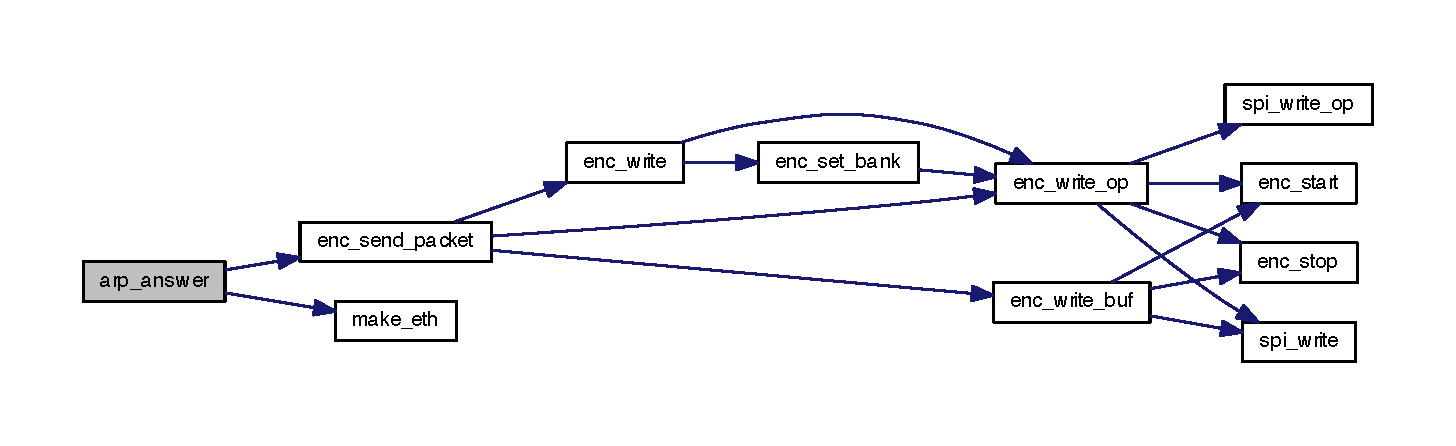
\includegraphics[width=350pt]{net_8h_a28773a34ece2b6d44dd567c8b110a4d0_cgraph}
\end{center}
\end{figure}


\hypertarget{net_8h_ae7ef39d9ed2b416c9fa575806e63ecb6}{\index{net.\+h@{net.\+h}!checksum@{checksum}}
\index{checksum@{checksum}!net.\+h@{net.\+h}}
\subsubsection[{checksum}]{\setlength{\rightskip}{0pt plus 5cm}uint16\+\_\+t checksum (
\begin{DoxyParamCaption}
\item[{uint8\+\_\+t $\ast$}]{buf, }
\item[{uint16\+\_\+t}]{len, }
\item[{uint8\+\_\+t}]{type}
\end{DoxyParamCaption}
)}}\label{net_8h_ae7ef39d9ed2b416c9fa575806e63ecb6}


checksum 


\begin{DoxyParams}{Parameters}
{\em buf} & buffer \\
\hline
{\em len} & length \\
\hline
{\em type} & type\\
\hline
\end{DoxyParams}
\begin{DoxyReturn}{Returns}
sum 
\end{DoxyReturn}


Definition at line 277 of file net.\+c.



References buf, I\+P\+\_\+\+P\+R\+O\+T\+O\+\_\+\+T\+C\+P\+\_\+\+V, and I\+P\+\_\+\+P\+R\+O\+T\+O\+\_\+\+U\+D\+P\+\_\+\+V.



Referenced by make\+\_\+ip(), and udp\+\_\+reply().

\hypertarget{net_8h_a373984d10afb4fc42dca8b356b39d245}{\index{net.\+h@{net.\+h}!echo\+\_\+reply@{echo\+\_\+reply}}
\index{echo\+\_\+reply@{echo\+\_\+reply}!net.\+h@{net.\+h}}
\subsubsection[{echo\+\_\+reply}]{\setlength{\rightskip}{0pt plus 5cm}void echo\+\_\+reply (
\begin{DoxyParamCaption}
\item[{uint8\+\_\+t $\ast$}]{buf, }
\item[{uint8\+\_\+t}]{len}
\end{DoxyParamCaption}
)}}\label{net_8h_a373984d10afb4fc42dca8b356b39d245}


make an echo answer (ping -\/ pong) if request 


\begin{DoxyParams}{Parameters}
{\em buf} & buffer \\
\hline
{\em len} & length of buffer \\
\hline
\end{DoxyParams}


Definition at line 158 of file net.\+c.



References enc\+\_\+send\+\_\+packet(), I\+C\+M\+P\+\_\+\+C\+H\+E\+C\+K\+S\+U\+M\+\_\+\+P, I\+C\+M\+P\+\_\+\+R\+E\+P\+L\+Y\+\_\+\+V, I\+C\+M\+P\+\_\+\+T\+Y\+P\+E\+\_\+\+P, make\+\_\+eth(), and make\+\_\+ip().



Referenced by main().



Here is the call graph for this function\+:
\nopagebreak
\begin{figure}[H]
\begin{center}
\leavevmode
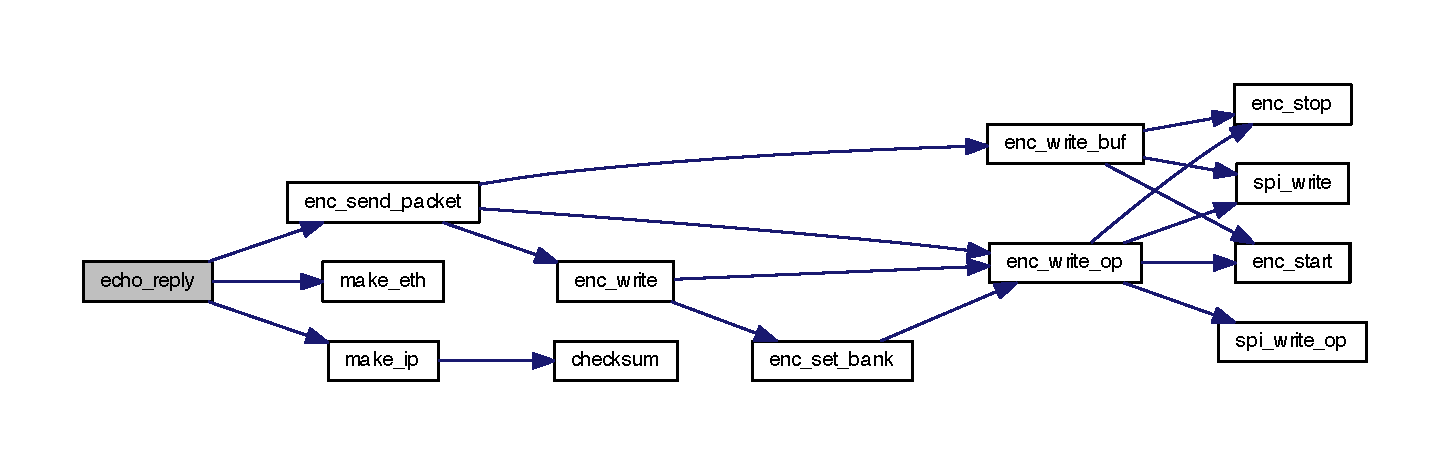
\includegraphics[width=350pt]{net_8h_a373984d10afb4fc42dca8b356b39d245_cgraph}
\end{center}
\end{figure}


\hypertarget{net_8h_adad2aa706a7d44a4993c12aeeb0f3ee5}{\index{net.\+h@{net.\+h}!eth\+\_\+arp@{eth\+\_\+arp}}
\index{eth\+\_\+arp@{eth\+\_\+arp}!net.\+h@{net.\+h}}
\subsubsection[{eth\+\_\+arp}]{\setlength{\rightskip}{0pt plus 5cm}uint8\+\_\+t eth\+\_\+arp (
\begin{DoxyParamCaption}
\item[{uint8\+\_\+t $\ast$}]{buf, }
\item[{uint8\+\_\+t}]{len}
\end{DoxyParamCaption}
)}}\label{net_8h_adad2aa706a7d44a4993c12aeeb0f3ee5}


make the network wirh arp 


\begin{DoxyParams}{Parameters}
{\em buf} & buffer \\
\hline
{\em len} & length of buffer\\
\hline
\end{DoxyParams}
\begin{DoxyReturn}{Returns}
return 1 if success, otherwise zero 
\end{DoxyReturn}


Definition at line 67 of file net.\+c.



References A\+R\+P\+\_\+\+D\+E\+S\+T\+\_\+\+I\+P\+\_\+\+P, E\+T\+H\+\_\+\+T\+Y\+P\+E\+\_\+\+H\+\_\+\+P, E\+T\+H\+\_\+\+T\+Y\+P\+E\+\_\+\+L\+\_\+\+P, E\+T\+H\+T\+Y\+P\+E\+\_\+\+A\+R\+P\+\_\+\+H\+\_\+\+V, E\+T\+H\+T\+Y\+P\+E\+\_\+\+A\+R\+P\+\_\+\+L\+\_\+\+V, and ipaddr.



Referenced by main().

\hypertarget{net_8h_a29b7bf9dc451b96400620066cfd4122a}{\index{net.\+h@{net.\+h}!eth\+\_\+ip@{eth\+\_\+ip}}
\index{eth\+\_\+ip@{eth\+\_\+ip}!net.\+h@{net.\+h}}
\subsubsection[{eth\+\_\+ip}]{\setlength{\rightskip}{0pt plus 5cm}uint8\+\_\+t eth\+\_\+ip (
\begin{DoxyParamCaption}
\item[{uint8\+\_\+t $\ast$}]{buf, }
\item[{uint8\+\_\+t}]{len}
\end{DoxyParamCaption}
)}}\label{net_8h_a29b7bf9dc451b96400620066cfd4122a}


make the network communication with ip address 


\begin{DoxyParams}{Parameters}
{\em buf} & buffer \\
\hline
{\em len} & length of buffer\\
\hline
\end{DoxyParams}
\begin{DoxyReturn}{Returns}
returns 1 if success, otherwise zero 
\end{DoxyReturn}


Definition at line 97 of file net.\+c.



References E\+T\+H\+\_\+\+T\+Y\+P\+E\+\_\+\+H\+\_\+\+P, E\+T\+H\+\_\+\+T\+Y\+P\+E\+\_\+\+L\+\_\+\+P, E\+T\+H\+T\+Y\+P\+E\+\_\+\+I\+P\+\_\+\+H\+\_\+\+V, E\+T\+H\+T\+Y\+P\+E\+\_\+\+I\+P\+\_\+\+L\+\_\+\+V, I\+P\+\_\+\+D\+E\+S\+T\+\_\+\+P, and ipaddr.



Referenced by main().

\hypertarget{net_8h_af8b6b03bdab2ed94c16fa6370cf806d6}{\index{net.\+h@{net.\+h}!make\+\_\+eth@{make\+\_\+eth}}
\index{make\+\_\+eth@{make\+\_\+eth}!net.\+h@{net.\+h}}
\subsubsection[{make\+\_\+eth}]{\setlength{\rightskip}{0pt plus 5cm}void make\+\_\+eth (
\begin{DoxyParamCaption}
\item[{uint8\+\_\+t $\ast$}]{buf}
\end{DoxyParamCaption}
)}}\label{net_8h_af8b6b03bdab2ed94c16fa6370cf806d6}


make the ethernet header 


\begin{DoxyParams}{Parameters}
{\em buf} & buffer \\
\hline
\end{DoxyParams}


Definition at line 225 of file net.\+c.



References E\+T\+H\+\_\+\+D\+E\+S\+T\+\_\+\+M\+A\+C, E\+T\+H\+\_\+\+S\+R\+C\+\_\+\+M\+A\+C, and macaddr.



Referenced by arp\+\_\+answer(), echo\+\_\+reply(), and udp\+\_\+reply().

\hypertarget{net_8h_a57c50aa78a3b5d2dc8d8fd21d7ced975}{\index{net.\+h@{net.\+h}!make\+\_\+ip@{make\+\_\+ip}}
\index{make\+\_\+ip@{make\+\_\+ip}!net.\+h@{net.\+h}}
\subsubsection[{make\+\_\+ip}]{\setlength{\rightskip}{0pt plus 5cm}void make\+\_\+ip (
\begin{DoxyParamCaption}
\item[{uint8\+\_\+t $\ast$}]{buf}
\end{DoxyParamCaption}
)}}\label{net_8h_a57c50aa78a3b5d2dc8d8fd21d7ced975}


make the ip header 


\begin{DoxyParams}{Parameters}
{\em buf} & \\
\hline
\end{DoxyParams}


Definition at line 242 of file net.\+c.



References checksum(), I\+P\+\_\+\+C\+H\+E\+C\+K\+S\+U\+M\+\_\+\+P, I\+P\+\_\+\+D\+E\+S\+T\+\_\+\+P, I\+P\+\_\+\+F\+L\+A\+G\+S\+\_\+\+P, I\+P\+\_\+\+H\+E\+A\+D\+E\+R\+\_\+\+L\+E\+N, I\+P\+\_\+\+P, I\+P\+\_\+\+S\+R\+C\+\_\+\+P, I\+P\+\_\+\+T\+T\+L\+\_\+\+P, and ipaddr.



Referenced by echo\+\_\+reply(), and udp\+\_\+reply().



Here is the call graph for this function\+:
\nopagebreak
\begin{figure}[H]
\begin{center}
\leavevmode
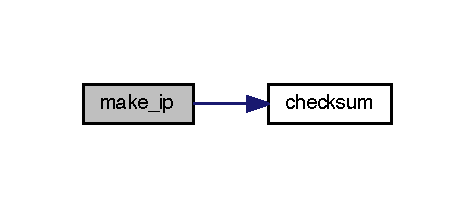
\includegraphics[width=228pt]{net_8h_a57c50aa78a3b5d2dc8d8fd21d7ced975_cgraph}
\end{center}
\end{figure}


\hypertarget{net_8h_ae66d6e0f4a7fee030d0b181873fd3c43}{\index{net.\+h@{net.\+h}!net\+\_\+init@{net\+\_\+init}}
\index{net\+\_\+init@{net\+\_\+init}!net.\+h@{net.\+h}}
\subsubsection[{net\+\_\+init}]{\setlength{\rightskip}{0pt plus 5cm}void net\+\_\+init (
\begin{DoxyParamCaption}
\item[{uint8\+\_\+t $\ast$}]{mymac, }
\item[{uint8\+\_\+t $\ast$}]{myip}
\end{DoxyParamCaption}
)}}\label{net_8h_ae66d6e0f4a7fee030d0b181873fd3c43}


initialize the network 


\begin{DoxyParams}{Parameters}
{\em mymac} & my mac address \\
\hline
{\em myip} & my ip address \\
\hline
\end{DoxyParams}


Definition at line 43 of file net.\+c.



References ipaddr, and macaddr.



Referenced by main().

\hypertarget{net_8h_ad6dd37c1e1e4f4a907f53c406a088cb3}{\index{net.\+h@{net.\+h}!udp\+\_\+reply@{udp\+\_\+reply}}
\index{udp\+\_\+reply@{udp\+\_\+reply}!net.\+h@{net.\+h}}
\subsubsection[{udp\+\_\+reply}]{\setlength{\rightskip}{0pt plus 5cm}void udp\+\_\+reply (
\begin{DoxyParamCaption}
\item[{uint8\+\_\+t $\ast$}]{buf, }
\item[{char $\ast$}]{data, }
\item[{uint8\+\_\+t}]{len, }
\item[{uint16\+\_\+t}]{port}
\end{DoxyParamCaption}
)}}\label{net_8h_ad6dd37c1e1e4f4a907f53c406a088cb3}


make the U\+D\+P protocol 


\begin{DoxyParams}{Parameters}
{\em buf} & buffer \\
\hline
{\em data} & data \\
\hline
{\em len} & length \\
\hline
{\em port} & port number \\
\hline
\end{DoxyParams}


Definition at line 182 of file net.\+c.



References checksum(), enc\+\_\+send\+\_\+packet(), E\+T\+H\+\_\+\+H\+E\+A\+D\+E\+R\+\_\+\+L\+E\+N, I\+P\+\_\+\+H\+E\+A\+D\+E\+R\+\_\+\+L\+E\+N, I\+P\+\_\+\+S\+R\+C\+\_\+\+P, I\+P\+\_\+\+T\+O\+T\+L\+E\+N\+\_\+\+H\+\_\+\+P, I\+P\+\_\+\+T\+O\+T\+L\+E\+N\+\_\+\+L\+\_\+\+P, make\+\_\+eth(), make\+\_\+ip(), U\+D\+P\+\_\+\+C\+H\+E\+C\+K\+S\+U\+M\+\_\+\+H\+\_\+\+P, U\+D\+P\+\_\+\+C\+H\+E\+C\+K\+S\+U\+M\+\_\+\+L\+\_\+\+P, U\+D\+P\+\_\+\+D\+A\+T\+A\+\_\+\+P, U\+D\+P\+\_\+\+D\+E\+S\+T\+\_\+\+P\+O\+R\+T\+\_\+\+H\+\_\+\+P, U\+D\+P\+\_\+\+D\+E\+S\+T\+\_\+\+P\+O\+R\+T\+\_\+\+L\+\_\+\+P, U\+D\+P\+\_\+\+H\+E\+A\+D\+E\+R\+\_\+\+L\+E\+N, U\+D\+P\+\_\+\+L\+E\+N\+\_\+\+H\+\_\+\+P, U\+D\+P\+\_\+\+L\+E\+N\+\_\+\+L\+\_\+\+P, U\+D\+P\+\_\+\+S\+R\+C\+\_\+\+P\+O\+R\+T\+\_\+\+H\+\_\+\+P, and U\+D\+P\+\_\+\+S\+R\+C\+\_\+\+P\+O\+R\+T\+\_\+\+L\+\_\+\+P.



Referenced by main().



Here is the call graph for this function\+:
\nopagebreak
\begin{figure}[H]
\begin{center}
\leavevmode
\includegraphics[width=350pt]{net_8h_ad6dd37c1e1e4f4a907f53c406a088cb3_cgraph}
\end{center}
\end{figure}



\hypertarget{spi_8c}{\section{driver/spi.c File Reference}
\label{spi_8c}\index{driver/spi.\+c@{driver/spi.\+c}}
}


driver for spi interface  


{\ttfamily \#include $<$driver/spi.\+h$>$}\\*
Include dependency graph for spi.\+c\+:
\nopagebreak
\begin{figure}[H]
\begin{center}
\leavevmode
\includegraphics[width=350pt]{spi_8c__incl}
\end{center}
\end{figure}
\subsection*{Functions}
\begin{DoxyCompactItemize}
\item 
void \hyperlink{spi_8c_ae909944aa85ae98323073c628be541aa}{spi\+\_\+init} (void)
\begin{DoxyCompactList}\small\item\em initialize S\+P\+I communication \end{DoxyCompactList}\item 
void \hyperlink{spi_8c_afd67d0a4eba1be3a38b0234274f477d8}{spi\+\_\+write\+\_\+op} (uint8\+\_\+t op, uint8\+\_\+t addr)
\begin{DoxyCompactList}\small\item\em write an operation to address \end{DoxyCompactList}\item 
void \hyperlink{spi_8c_a656cafaeae25fbe893fb580a06360dba}{spi\+\_\+write} (uint8\+\_\+t data)
\begin{DoxyCompactList}\small\item\em write the data to S\+P\+I \end{DoxyCompactList}\item 
uint8\+\_\+t \hyperlink{spi_8c_a14e73be3886cad229afafebc98c4c66d}{spi\+\_\+read\+\_\+addr} (uint8\+\_\+t addr)
\begin{DoxyCompactList}\small\item\em read from address \end{DoxyCompactList}\item 
uint8\+\_\+t \hyperlink{spi_8c_a82a4ec3bb6d4bdaf7453f2ccc19b2243}{spi\+\_\+read} (void)
\begin{DoxyCompactList}\small\item\em read from S\+P\+I data register \end{DoxyCompactList}\end{DoxyCompactItemize}


\subsection{Detailed Description}
driver for spi interface 

\begin{DoxyAuthor}{Author}
M. Ozgan, \href{mailto:mozgan@mozgan.org}{\tt mozgan@mozgan.\+org} 
\end{DoxyAuthor}
\begin{DoxyVersion}{Version}
0.\+1 
\end{DoxyVersion}
\begin{DoxyDate}{Date}
20.\+08.\+2013 14\+:52\+:49 
\end{DoxyDate}
\begin{DoxyParagraph}{Compiler}
gcc (on Mac, and 4.\+4\+B\+S\+D) 
\end{DoxyParagraph}
\begin{DoxyParagraph}{Company}
T\+U Wien 
\end{DoxyParagraph}


\begin{DoxyRefDesc}{Bug}
\item[\hyperlink{bug__bug000011}{Bug}]none \end{DoxyRefDesc}
\begin{DoxyRefDesc}{Todo}
\item[\hyperlink{todo__todo000011}{Todo}]none \end{DoxyRefDesc}


Definition in file \hyperlink{spi_8c_source}{spi.\+c}.



\subsection{Function Documentation}
\hypertarget{spi_8c_ae909944aa85ae98323073c628be541aa}{\index{spi.\+c@{spi.\+c}!spi\+\_\+init@{spi\+\_\+init}}
\index{spi\+\_\+init@{spi\+\_\+init}!spi.\+c@{spi.\+c}}
\subsubsection[{spi\+\_\+init}]{\setlength{\rightskip}{0pt plus 5cm}void spi\+\_\+init (
\begin{DoxyParamCaption}
\item[{void}]{}
\end{DoxyParamCaption}
)}}\label{spi_8c_ae909944aa85ae98323073c628be541aa}


initialize S\+P\+I communication 



Definition at line 33 of file spi.\+c.



References S\+P\+I\+\_\+\+C\+O\+N\+T\+R\+O\+L\+\_\+\+R\+E\+G, S\+P\+I\+\_\+\+D\+D\+R, S\+P\+I\+\_\+\+D\+O\+U\+B\+L\+E\+\_\+\+S\+P\+E\+E\+D, S\+P\+I\+\_\+\+E\+N\+A\+B\+L\+E, S\+P\+I\+\_\+\+M\+A\+S\+T\+E\+R, S\+P\+I\+\_\+\+M\+I\+S\+O, S\+P\+I\+\_\+\+M\+O\+S\+I, S\+P\+I\+\_\+\+P\+O\+R\+T, S\+P\+I\+\_\+\+S\+C\+K, S\+P\+I\+\_\+\+S\+S, and S\+P\+I\+\_\+\+S\+T\+A\+T\+U\+S\+\_\+\+R\+E\+G.



Referenced by enc\+\_\+init().

\hypertarget{spi_8c_a82a4ec3bb6d4bdaf7453f2ccc19b2243}{\index{spi.\+c@{spi.\+c}!spi\+\_\+read@{spi\+\_\+read}}
\index{spi\+\_\+read@{spi\+\_\+read}!spi.\+c@{spi.\+c}}
\subsubsection[{spi\+\_\+read}]{\setlength{\rightskip}{0pt plus 5cm}uint8\+\_\+t spi\+\_\+read (
\begin{DoxyParamCaption}
\item[{void}]{}
\end{DoxyParamCaption}
)}}\label{spi_8c_a82a4ec3bb6d4bdaf7453f2ccc19b2243}


read from S\+P\+I data register 

\begin{DoxyReturn}{Returns}
value of S\+P\+I data register 
\end{DoxyReturn}


Definition at line 102 of file spi.\+c.



Referenced by enc\+\_\+read\+\_\+buf().

\hypertarget{spi_8c_a14e73be3886cad229afafebc98c4c66d}{\index{spi.\+c@{spi.\+c}!spi\+\_\+read\+\_\+addr@{spi\+\_\+read\+\_\+addr}}
\index{spi\+\_\+read\+\_\+addr@{spi\+\_\+read\+\_\+addr}!spi.\+c@{spi.\+c}}
\subsubsection[{spi\+\_\+read\+\_\+addr}]{\setlength{\rightskip}{0pt plus 5cm}uint8\+\_\+t spi\+\_\+read\+\_\+addr (
\begin{DoxyParamCaption}
\item[{uint8\+\_\+t}]{addr}
\end{DoxyParamCaption}
)}}\label{spi_8c_a14e73be3886cad229afafebc98c4c66d}


read from address 


\begin{DoxyParams}{Parameters}
{\em addr} & address\\
\hline
\end{DoxyParams}
\begin{DoxyReturn}{Returns}

\end{DoxyReturn}


Definition at line 84 of file spi.\+c.



Referenced by enc\+\_\+read\+\_\+op().

\hypertarget{spi_8c_a656cafaeae25fbe893fb580a06360dba}{\index{spi.\+c@{spi.\+c}!spi\+\_\+write@{spi\+\_\+write}}
\index{spi\+\_\+write@{spi\+\_\+write}!spi.\+c@{spi.\+c}}
\subsubsection[{spi\+\_\+write}]{\setlength{\rightskip}{0pt plus 5cm}void spi\+\_\+write (
\begin{DoxyParamCaption}
\item[{uint8\+\_\+t}]{data}
\end{DoxyParamCaption}
)}}\label{spi_8c_a656cafaeae25fbe893fb580a06360dba}


write the data to S\+P\+I 


\begin{DoxyParams}{Parameters}
{\em data} & data \\
\hline
\end{DoxyParams}


Definition at line 68 of file spi.\+c.



References S\+P\+I\+\_\+\+I\+N\+T\+\_\+\+F\+L\+A\+G, and S\+P\+I\+\_\+\+S\+T\+A\+T\+U\+S\+\_\+\+R\+E\+G.



Referenced by enc\+\_\+read\+\_\+buf(), enc\+\_\+read\+\_\+op(), enc\+\_\+write\+\_\+buf(), and enc\+\_\+write\+\_\+op().

\hypertarget{spi_8c_afd67d0a4eba1be3a38b0234274f477d8}{\index{spi.\+c@{spi.\+c}!spi\+\_\+write\+\_\+op@{spi\+\_\+write\+\_\+op}}
\index{spi\+\_\+write\+\_\+op@{spi\+\_\+write\+\_\+op}!spi.\+c@{spi.\+c}}
\subsubsection[{spi\+\_\+write\+\_\+op}]{\setlength{\rightskip}{0pt plus 5cm}void spi\+\_\+write\+\_\+op (
\begin{DoxyParamCaption}
\item[{uint8\+\_\+t}]{op, }
\item[{uint8\+\_\+t}]{addr}
\end{DoxyParamCaption}
)}}\label{spi_8c_afd67d0a4eba1be3a38b0234274f477d8}


write an operation to address 


\begin{DoxyParams}{Parameters}
{\em op} & operation \\
\hline
{\em addr} & address \\
\hline
\end{DoxyParams}


Definition at line 54 of file spi.\+c.



References A\+D\+D\+R\+\_\+\+M\+A\+S\+K, S\+P\+I\+\_\+\+D\+A\+T\+A\+\_\+\+R\+E\+G, S\+P\+I\+\_\+\+I\+N\+T\+\_\+\+F\+L\+A\+G, and S\+P\+I\+\_\+\+S\+T\+A\+T\+U\+S\+\_\+\+R\+E\+G.



Referenced by enc\+\_\+read\+\_\+op(), and enc\+\_\+write\+\_\+op().


\hypertarget{spi_8h}{\section{driver/spi.h File Reference}
\label{spi_8h}\index{driver/spi.\+h@{driver/spi.\+h}}
}


header file for spi interface  


{\ttfamily \#include $<$board/freq.\+h$>$}\\*
{\ttfamily \#include $<$device/atmega16.\+h$>$}\\*
{\ttfamily \#include $<$device/enc28j60.\+h$>$}\\*
Include dependency graph for spi.\+h\+:
\nopagebreak
\begin{figure}[H]
\begin{center}
\leavevmode
\includegraphics[width=350pt]{spi_8h__incl}
\end{center}
\end{figure}
This graph shows which files directly or indirectly include this file\+:
\nopagebreak
\begin{figure}[H]
\begin{center}
\leavevmode
\includegraphics[width=246pt]{spi_8h__dep__incl}
\end{center}
\end{figure}
\subsection*{Functions}
\begin{DoxyCompactItemize}
\item 
void \hyperlink{spi_8h_ae909944aa85ae98323073c628be541aa}{spi\+\_\+init} (void)
\begin{DoxyCompactList}\small\item\em initialize S\+P\+I communication \end{DoxyCompactList}\item 
void \hyperlink{spi_8h_a02743643e4a5d72bcff3f5d3f9f16a5b}{spi\+\_\+write\+\_\+op} (uint8\+\_\+t, uint8\+\_\+t)
\begin{DoxyCompactList}\small\item\em write an operation to address \end{DoxyCompactList}\item 
void \hyperlink{spi_8h_a96e2d807e16c3fb283b044ea0e90e7b2}{spi\+\_\+write} (uint8\+\_\+t)
\begin{DoxyCompactList}\small\item\em write the data to S\+P\+I \end{DoxyCompactList}\item 
uint8\+\_\+t \hyperlink{spi_8h_a1d77032a366b1c4e5d6e9f49712b9518}{spi\+\_\+read\+\_\+addr} (uint8\+\_\+t)
\begin{DoxyCompactList}\small\item\em read from address \end{DoxyCompactList}\item 
uint8\+\_\+t \hyperlink{spi_8h_a82a4ec3bb6d4bdaf7453f2ccc19b2243}{spi\+\_\+read} (void)
\begin{DoxyCompactList}\small\item\em read from S\+P\+I data register \end{DoxyCompactList}\end{DoxyCompactItemize}


\subsection{Detailed Description}
header file for spi interface 

\begin{DoxyAuthor}{Author}
M. Ozgan, \href{mailto:mozgan@mozgan.org}{\tt mozgan@mozgan.\+org} 
\end{DoxyAuthor}
\begin{DoxyVersion}{Version}
0.\+1 
\end{DoxyVersion}
\begin{DoxyDate}{Date}
20.\+08.\+2013 14\+:52\+:02 
\end{DoxyDate}
\begin{DoxyParagraph}{Compiler}
gcc (on Mac, G\+N\+U/\+Linux and 4.\+4\+B\+S\+D) 
\end{DoxyParagraph}
\begin{DoxyParagraph}{Company}
T\+U Wien 
\end{DoxyParagraph}


\begin{DoxyRefDesc}{Bug}
\item[\hyperlink{bug__bug000012}{Bug}]none \end{DoxyRefDesc}
\begin{DoxyRefDesc}{Todo}
\item[\hyperlink{todo__todo000012}{Todo}]none \end{DoxyRefDesc}


Definition in file \hyperlink{spi_8h_source}{spi.\+h}.



\subsection{Function Documentation}
\hypertarget{spi_8h_ae909944aa85ae98323073c628be541aa}{\index{spi.\+h@{spi.\+h}!spi\+\_\+init@{spi\+\_\+init}}
\index{spi\+\_\+init@{spi\+\_\+init}!spi.\+h@{spi.\+h}}
\subsubsection[{spi\+\_\+init}]{\setlength{\rightskip}{0pt plus 5cm}void spi\+\_\+init (
\begin{DoxyParamCaption}
\item[{void}]{}
\end{DoxyParamCaption}
)}}\label{spi_8h_ae909944aa85ae98323073c628be541aa}


initialize S\+P\+I communication 



Definition at line 33 of file spi.\+c.



References S\+P\+I\+\_\+\+C\+O\+N\+T\+R\+O\+L\+\_\+\+R\+E\+G, S\+P\+I\+\_\+\+D\+D\+R, S\+P\+I\+\_\+\+D\+O\+U\+B\+L\+E\+\_\+\+S\+P\+E\+E\+D, S\+P\+I\+\_\+\+E\+N\+A\+B\+L\+E, S\+P\+I\+\_\+\+M\+A\+S\+T\+E\+R, S\+P\+I\+\_\+\+M\+I\+S\+O, S\+P\+I\+\_\+\+M\+O\+S\+I, S\+P\+I\+\_\+\+P\+O\+R\+T, S\+P\+I\+\_\+\+S\+C\+K, S\+P\+I\+\_\+\+S\+S, and S\+P\+I\+\_\+\+S\+T\+A\+T\+U\+S\+\_\+\+R\+E\+G.



Referenced by enc\+\_\+init().

\hypertarget{spi_8h_a82a4ec3bb6d4bdaf7453f2ccc19b2243}{\index{spi.\+h@{spi.\+h}!spi\+\_\+read@{spi\+\_\+read}}
\index{spi\+\_\+read@{spi\+\_\+read}!spi.\+h@{spi.\+h}}
\subsubsection[{spi\+\_\+read}]{\setlength{\rightskip}{0pt plus 5cm}uint8\+\_\+t spi\+\_\+read (
\begin{DoxyParamCaption}
\item[{void}]{}
\end{DoxyParamCaption}
)}}\label{spi_8h_a82a4ec3bb6d4bdaf7453f2ccc19b2243}


read from S\+P\+I data register 

\begin{DoxyReturn}{Returns}
value of S\+P\+I data register 
\end{DoxyReturn}


Definition at line 102 of file spi.\+c.



Referenced by enc\+\_\+read\+\_\+buf().

\hypertarget{spi_8h_a1d77032a366b1c4e5d6e9f49712b9518}{\index{spi.\+h@{spi.\+h}!spi\+\_\+read\+\_\+addr@{spi\+\_\+read\+\_\+addr}}
\index{spi\+\_\+read\+\_\+addr@{spi\+\_\+read\+\_\+addr}!spi.\+h@{spi.\+h}}
\subsubsection[{spi\+\_\+read\+\_\+addr}]{\setlength{\rightskip}{0pt plus 5cm}uint8\+\_\+t spi\+\_\+read\+\_\+addr (
\begin{DoxyParamCaption}
\item[{uint8\+\_\+t}]{addr}
\end{DoxyParamCaption}
)}}\label{spi_8h_a1d77032a366b1c4e5d6e9f49712b9518}


read from address 


\begin{DoxyParams}{Parameters}
{\em addr} & address\\
\hline
\end{DoxyParams}
\begin{DoxyReturn}{Returns}

\end{DoxyReturn}


Definition at line 84 of file spi.\+c.



Referenced by enc\+\_\+read\+\_\+op().

\hypertarget{spi_8h_a96e2d807e16c3fb283b044ea0e90e7b2}{\index{spi.\+h@{spi.\+h}!spi\+\_\+write@{spi\+\_\+write}}
\index{spi\+\_\+write@{spi\+\_\+write}!spi.\+h@{spi.\+h}}
\subsubsection[{spi\+\_\+write}]{\setlength{\rightskip}{0pt plus 5cm}void spi\+\_\+write (
\begin{DoxyParamCaption}
\item[{uint8\+\_\+t}]{data}
\end{DoxyParamCaption}
)}}\label{spi_8h_a96e2d807e16c3fb283b044ea0e90e7b2}


write the data to S\+P\+I 


\begin{DoxyParams}{Parameters}
{\em data} & data \\
\hline
\end{DoxyParams}


Definition at line 68 of file spi.\+c.



References S\+P\+I\+\_\+\+I\+N\+T\+\_\+\+F\+L\+A\+G, and S\+P\+I\+\_\+\+S\+T\+A\+T\+U\+S\+\_\+\+R\+E\+G.



Referenced by enc\+\_\+read\+\_\+buf(), enc\+\_\+read\+\_\+op(), enc\+\_\+write\+\_\+buf(), and enc\+\_\+write\+\_\+op().

\hypertarget{spi_8h_a02743643e4a5d72bcff3f5d3f9f16a5b}{\index{spi.\+h@{spi.\+h}!spi\+\_\+write\+\_\+op@{spi\+\_\+write\+\_\+op}}
\index{spi\+\_\+write\+\_\+op@{spi\+\_\+write\+\_\+op}!spi.\+h@{spi.\+h}}
\subsubsection[{spi\+\_\+write\+\_\+op}]{\setlength{\rightskip}{0pt plus 5cm}void spi\+\_\+write\+\_\+op (
\begin{DoxyParamCaption}
\item[{uint8\+\_\+t}]{op, }
\item[{uint8\+\_\+t}]{addr}
\end{DoxyParamCaption}
)}}\label{spi_8h_a02743643e4a5d72bcff3f5d3f9f16a5b}


write an operation to address 


\begin{DoxyParams}{Parameters}
{\em op} & operation \\
\hline
{\em addr} & address \\
\hline
\end{DoxyParams}


Definition at line 54 of file spi.\+c.



References A\+D\+D\+R\+\_\+\+M\+A\+S\+K, S\+P\+I\+\_\+\+D\+A\+T\+A\+\_\+\+R\+E\+G, S\+P\+I\+\_\+\+I\+N\+T\+\_\+\+F\+L\+A\+G, and S\+P\+I\+\_\+\+S\+T\+A\+T\+U\+S\+\_\+\+R\+E\+G.



Referenced by enc\+\_\+read\+\_\+op(), and enc\+\_\+write\+\_\+op().


\hypertarget{timer0_8c}{\section{driver/timer0.c File Reference}
\label{timer0_8c}\index{driver/timer0.\+c@{driver/timer0.\+c}}
}


driver of timer/counter 0  


{\ttfamily \#include $<$driver/timer0.\+h$>$}\\*
{\ttfamily \#include $<$driver/leds.\+h$>$}\\*
Include dependency graph for timer0.\+c\+:
\nopagebreak
\begin{figure}[H]
\begin{center}
\leavevmode
\includegraphics[width=350pt]{timer0_8c__incl}
\end{center}
\end{figure}
\subsection*{Functions}
\begin{DoxyCompactItemize}
\item 
void \hyperlink{timer0_8c_abf7b90cef43b44a249288fbd506fc711}{timer0\+\_\+init\+\_\+f} (uint16\+\_\+t \hyperlink{main_8c_a74796ad69e9a5ee4a0448582ba5b1bb7}{freq}, void($\ast$call\+\_\+back)(void))
\begin{DoxyCompactList}\small\item\em initialize timer/counter 0 with frequency \end{DoxyCompactList}\item 
void \hyperlink{timer0_8c_a813c0dbc5c9118e5c6ef1203b73aced3}{timer0\+\_\+stop} (void)
\begin{DoxyCompactList}\small\item\em stop the timer 0 \end{DoxyCompactList}\item 
\hyperlink{timer0_8c_ada481aa6f700b24e2f7cb2bbb6a0227a}{I\+S\+R} (T\+I\+M\+E\+R0\+\_\+\+C\+O\+M\+P\+\_\+vect)
\begin{DoxyCompactList}\small\item\em Interrupt for timer/counter 0 of campare output match mode. \end{DoxyCompactList}\end{DoxyCompactItemize}
\subsection*{Variables}
\begin{DoxyCompactItemize}
\item 
volatile int \hyperlink{timer0_8c_a9c245a703414df52e903e8df8857392a}{cnt0} = 0
\end{DoxyCompactItemize}


\subsection{Detailed Description}
driver of timer/counter 0 

\begin{DoxyAuthor}{Author}
M. Ozgan, \href{mailto:mozgan@mozgan.org}{\tt mozgan@mozgan.\+org} 
\end{DoxyAuthor}
\begin{DoxyVersion}{Version}
0.\+2 
\end{DoxyVersion}
\begin{DoxyDate}{Date}
19.\+08.\+2013 15\+:55\+:03 
\end{DoxyDate}
\begin{DoxyParagraph}{Compiler}
gcc (on Mac, and 4.\+4\+B\+S\+D) 
\end{DoxyParagraph}
\begin{DoxyParagraph}{Company}
T\+U Wien 
\end{DoxyParagraph}


\begin{DoxyRefDesc}{Bug}
\item[\hyperlink{bug__bug000013}{Bug}]none \end{DoxyRefDesc}
\begin{DoxyRefDesc}{Todo}
\item[\hyperlink{todo__todo000013}{Todo}]none \end{DoxyRefDesc}


Definition in file \hyperlink{timer0_8c_source}{timer0.\+c}.



\subsection{Function Documentation}
\hypertarget{timer0_8c_ada481aa6f700b24e2f7cb2bbb6a0227a}{\index{timer0.\+c@{timer0.\+c}!I\+S\+R@{I\+S\+R}}
\index{I\+S\+R@{I\+S\+R}!timer0.\+c@{timer0.\+c}}
\subsubsection[{I\+S\+R}]{\setlength{\rightskip}{0pt plus 5cm}I\+S\+R (
\begin{DoxyParamCaption}
\item[{T\+I\+M\+E\+R0\+\_\+\+C\+O\+M\+P\+\_\+vect}]{}
\end{DoxyParamCaption}
)}}\label{timer0_8c_ada481aa6f700b24e2f7cb2bbb6a0227a}


Interrupt for timer/counter 0 of campare output match mode. 


\begin{DoxyParams}{Parameters}
{\em T\+I\+M\+E\+R0\+\_\+\+C\+O\+M\+P\+\_\+vect} & Interrupt vector \\
\hline
\end{DoxyParams}


Definition at line 78 of file timer0.\+c.



References cnt0, int\+\_\+cnt0, N\+U\+L\+L, and timer0\+\_\+handler.

\hypertarget{timer0_8c_abf7b90cef43b44a249288fbd506fc711}{\index{timer0.\+c@{timer0.\+c}!timer0\+\_\+init\+\_\+f@{timer0\+\_\+init\+\_\+f}}
\index{timer0\+\_\+init\+\_\+f@{timer0\+\_\+init\+\_\+f}!timer0.\+c@{timer0.\+c}}
\subsubsection[{timer0\+\_\+init\+\_\+f}]{\setlength{\rightskip}{0pt plus 5cm}void timer0\+\_\+init\+\_\+f (
\begin{DoxyParamCaption}
\item[{uint16\+\_\+t}]{freq, }
\item[{void($\ast$)(void)}]{call\+\_\+back}
\end{DoxyParamCaption}
)}}\label{timer0_8c_abf7b90cef43b44a249288fbd506fc711}


initialize timer/counter 0 with frequency 


\begin{DoxyParams}{Parameters}
{\em freq} & timer frequency \\
\hline
{\em call\+\_\+back} & if timer interrupt request, returns to call\+\_\+back function \\
\hline
\end{DoxyParams}


Definition at line 39 of file timer0.\+c.



References F\+\_\+\+C\+P\+U, int\+\_\+cnt0, T\+I\+M\+E\+R0\+\_\+\+C\+N\+T, T\+I\+M\+E\+R0\+\_\+\+C\+T\+C, timer0\+\_\+handler, T\+I\+M\+E\+R0\+\_\+\+O\+C\+R, T\+I\+M\+E\+R0\+\_\+\+P\+R\+E\+S\+\_\+256, T\+I\+M\+E\+R0\+\_\+\+T\+C\+C\+R, T\+I\+M\+E\+R\+\_\+\+I\+N\+T\+\_\+\+F\+L\+G, and T\+I\+M\+E\+R\+\_\+\+I\+N\+T\+\_\+\+M\+A\+S\+K.

\hypertarget{timer0_8c_a813c0dbc5c9118e5c6ef1203b73aced3}{\index{timer0.\+c@{timer0.\+c}!timer0\+\_\+stop@{timer0\+\_\+stop}}
\index{timer0\+\_\+stop@{timer0\+\_\+stop}!timer0.\+c@{timer0.\+c}}
\subsubsection[{timer0\+\_\+stop}]{\setlength{\rightskip}{0pt plus 5cm}void timer0\+\_\+stop (
\begin{DoxyParamCaption}
\item[{void}]{}
\end{DoxyParamCaption}
)}}\label{timer0_8c_a813c0dbc5c9118e5c6ef1203b73aced3}


stop the timer 0 



Definition at line 68 of file timer0.\+c.



References T\+I\+M\+E\+R0\+\_\+\+N\+O\+\_\+\+C\+L\+K, and T\+I\+M\+E\+R0\+\_\+\+T\+C\+C\+R.



\subsection{Variable Documentation}
\hypertarget{timer0_8c_a9c245a703414df52e903e8df8857392a}{\index{timer0.\+c@{timer0.\+c}!cnt0@{cnt0}}
\index{cnt0@{cnt0}!timer0.\+c@{timer0.\+c}}
\subsubsection[{cnt0}]{\setlength{\rightskip}{0pt plus 5cm}volatile int cnt0 = 0}}\label{timer0_8c_a9c245a703414df52e903e8df8857392a}


Definition at line 30 of file timer0.\+c.



Referenced by I\+S\+R().


\hypertarget{timer0_8h}{\section{driver/timer0.h File Reference}
\label{timer0_8h}\index{driver/timer0.\+h@{driver/timer0.\+h}}
}


specific header file for timer/counter 0  


{\ttfamily \#include $<$board/freq.\+h$>$}\\*
{\ttfamily \#include $<$include/common.\+h$>$}\\*
Include dependency graph for timer0.\+h\+:
\nopagebreak
\begin{figure}[H]
\begin{center}
\leavevmode
\includegraphics[width=350pt]{timer0_8h__incl}
\end{center}
\end{figure}
This graph shows which files directly or indirectly include this file\+:
\nopagebreak
\begin{figure}[H]
\begin{center}
\leavevmode
\includegraphics[width=153pt]{timer0_8h__dep__incl}
\end{center}
\end{figure}
\subsection*{Functions}
\begin{DoxyCompactItemize}
\item 
void \hyperlink{timer0_8h_a9a3f7b6014a4ecdca7559692b40bf775}{timer0\+\_\+init\+\_\+f} (uint16\+\_\+t, void($\ast$)(void))
\begin{DoxyCompactList}\small\item\em initialize timer/counter 0 with frequency \end{DoxyCompactList}\item 
void \hyperlink{timer0_8h_a813c0dbc5c9118e5c6ef1203b73aced3}{timer0\+\_\+stop} (void)
\begin{DoxyCompactList}\small\item\em stop the timer 0 \end{DoxyCompactList}\end{DoxyCompactItemize}
\subsection*{Variables}
\begin{DoxyCompactItemize}
\item 
uint16\+\_\+t \hyperlink{timer0_8h_ab2b9d07ca040864058eb11c1c317489f}{int\+\_\+cnt0}
\item 
void($\ast$ \hyperlink{timer0_8h_ae6cf6e76e3ec6d8493d00da37ec2db6e}{timer0\+\_\+handler} )(void)
\end{DoxyCompactItemize}


\subsection{Detailed Description}
specific header file for timer/counter 0 

\begin{DoxyAuthor}{Author}
M. Ozgan, \href{mailto:mozgan@mozgan.org}{\tt mozgan@mozgan.\+org} 
\end{DoxyAuthor}
\begin{DoxyVersion}{Version}
0.\+2 
\end{DoxyVersion}
\begin{DoxyDate}{Date}
19.\+08.\+2013 15\+:54\+:58 
\end{DoxyDate}
\begin{DoxyParagraph}{Compiler}
gcc (on Mac, and 4.\+4\+B\+S\+D) 
\end{DoxyParagraph}
\begin{DoxyParagraph}{Company}
T\+U Wien 
\end{DoxyParagraph}


\begin{DoxyRefDesc}{Bug}
\item[\hyperlink{bug__bug000014}{Bug}]none \end{DoxyRefDesc}
\begin{DoxyRefDesc}{Todo}
\item[\hyperlink{todo__todo000014}{Todo}]none \end{DoxyRefDesc}


Definition in file \hyperlink{timer0_8h_source}{timer0.\+h}.



\subsection{Function Documentation}
\hypertarget{timer0_8h_a9a3f7b6014a4ecdca7559692b40bf775}{\index{timer0.\+h@{timer0.\+h}!timer0\+\_\+init\+\_\+f@{timer0\+\_\+init\+\_\+f}}
\index{timer0\+\_\+init\+\_\+f@{timer0\+\_\+init\+\_\+f}!timer0.\+h@{timer0.\+h}}
\subsubsection[{timer0\+\_\+init\+\_\+f}]{\setlength{\rightskip}{0pt plus 5cm}void timer0\+\_\+init\+\_\+f (
\begin{DoxyParamCaption}
\item[{uint16\+\_\+t}]{freq, }
\item[{void($\ast$)(void)}]{call\+\_\+back}
\end{DoxyParamCaption}
)}}\label{timer0_8h_a9a3f7b6014a4ecdca7559692b40bf775}


initialize timer/counter 0 with frequency 


\begin{DoxyParams}{Parameters}
{\em freq} & timer frequency \\
\hline
{\em call\+\_\+back} & if timer interrupt request, returns to call\+\_\+back function \\
\hline
\end{DoxyParams}


Definition at line 39 of file timer0.\+c.



References F\+\_\+\+C\+P\+U, int\+\_\+cnt0, T\+I\+M\+E\+R0\+\_\+\+C\+N\+T, T\+I\+M\+E\+R0\+\_\+\+C\+T\+C, timer0\+\_\+handler, T\+I\+M\+E\+R0\+\_\+\+O\+C\+R, T\+I\+M\+E\+R0\+\_\+\+P\+R\+E\+S\+\_\+256, T\+I\+M\+E\+R0\+\_\+\+T\+C\+C\+R, T\+I\+M\+E\+R\+\_\+\+I\+N\+T\+\_\+\+F\+L\+G, and T\+I\+M\+E\+R\+\_\+\+I\+N\+T\+\_\+\+M\+A\+S\+K.

\hypertarget{timer0_8h_a813c0dbc5c9118e5c6ef1203b73aced3}{\index{timer0.\+h@{timer0.\+h}!timer0\+\_\+stop@{timer0\+\_\+stop}}
\index{timer0\+\_\+stop@{timer0\+\_\+stop}!timer0.\+h@{timer0.\+h}}
\subsubsection[{timer0\+\_\+stop}]{\setlength{\rightskip}{0pt plus 5cm}void timer0\+\_\+stop (
\begin{DoxyParamCaption}
\item[{void}]{}
\end{DoxyParamCaption}
)}}\label{timer0_8h_a813c0dbc5c9118e5c6ef1203b73aced3}


stop the timer 0 



Definition at line 68 of file timer0.\+c.



References T\+I\+M\+E\+R0\+\_\+\+N\+O\+\_\+\+C\+L\+K, and T\+I\+M\+E\+R0\+\_\+\+T\+C\+C\+R.



\subsection{Variable Documentation}
\hypertarget{timer0_8h_ab2b9d07ca040864058eb11c1c317489f}{\index{timer0.\+h@{timer0.\+h}!int\+\_\+cnt0@{int\+\_\+cnt0}}
\index{int\+\_\+cnt0@{int\+\_\+cnt0}!timer0.\+h@{timer0.\+h}}
\subsubsection[{int\+\_\+cnt0}]{\setlength{\rightskip}{0pt plus 5cm}uint16\+\_\+t int\+\_\+cnt0}}\label{timer0_8h_ab2b9d07ca040864058eb11c1c317489f}
timer 0 interrupt counter 

Definition at line 33 of file timer0.\+h.



Referenced by I\+S\+R(), and timer0\+\_\+init\+\_\+f().

\hypertarget{timer0_8h_ae6cf6e76e3ec6d8493d00da37ec2db6e}{\index{timer0.\+h@{timer0.\+h}!timer0\+\_\+handler@{timer0\+\_\+handler}}
\index{timer0\+\_\+handler@{timer0\+\_\+handler}!timer0.\+h@{timer0.\+h}}
\subsubsection[{timer0\+\_\+handler}]{\setlength{\rightskip}{0pt plus 5cm}void($\ast$ timer0\+\_\+handler)(void)}}\label{timer0_8h_ae6cf6e76e3ec6d8493d00da37ec2db6e}
call back function from interrupt 

Definition at line 37 of file timer0.\+h.



Referenced by I\+S\+R(), and timer0\+\_\+init\+\_\+f().


\hypertarget{common_8h}{\section{include/common.h File Reference}
\label{common_8h}\index{include/common.\+h@{include/common.\+h}}
}


some useful definitions  


{\ttfamily \#include $<$stdbool.\+h$>$}\\*
Include dependency graph for common.\+h\+:
\nopagebreak
\begin{figure}[H]
\begin{center}
\leavevmode
\includegraphics[width=188pt]{common_8h__incl}
\end{center}
\end{figure}
This graph shows which files directly or indirectly include this file\+:
\nopagebreak
\begin{figure}[H]
\begin{center}
\leavevmode
\includegraphics[width=350pt]{common_8h__dep__incl}
\end{center}
\end{figure}
\subsection*{Macros}
\begin{DoxyCompactItemize}
\item 
\#define \hyperlink{common_8h_a74e75242132eaabbc1c512488a135926}{M\+I\+N}(x, y)~(((x) $<$ (y)) ? (x) \+: (y))
\begin{DoxyCompactList}\small\item\em find minimum \end{DoxyCompactList}\item 
\#define \hyperlink{common_8h_aacc3ee1a7f283f8ef65cea31f4436a95}{M\+A\+X}(x, y)~(((x) $>$ (y)) ? (x) \+: (y))
\begin{DoxyCompactList}\small\item\em find maximum \end{DoxyCompactList}\item 
\#define \hyperlink{common_8h_aa8cecfc5c5c054d2875c03e77b7be15d}{T\+R\+U\+E}~(\hyperlink{stdbool_8h_abb452686968e48b67397da5f97445f5b}{bool})(1)
\item 
\#define \hyperlink{common_8h_aa93f0eb578d23995850d61f7d61c55c1}{F\+A\+L\+S\+E}~(\hyperlink{stdbool_8h_abb452686968e48b67397da5f97445f5b}{bool})(0)
\item 
\#define \hyperlink{common_8h_a41f9c5fb8b08eb5dc3edce4dcb37fee7}{true}~(\hyperlink{stdbool_8h_abb452686968e48b67397da5f97445f5b}{bool})(1)
\item 
\#define \hyperlink{common_8h_a65e9886d74aaee76545e83dd09011727}{false}~(\hyperlink{stdbool_8h_abb452686968e48b67397da5f97445f5b}{bool})(0)
\item 
\#define \hyperlink{common_8h_a070d2ce7b6bb7e5c05602aa8c308d0c4}{N\+U\+L\+L}~(void $\ast$)(0)
\end{DoxyCompactItemize}


\subsection{Detailed Description}
some useful definitions 

\begin{DoxyAuthor}{Author}
M. Ozgan, \href{mailto:mozgan@mozgan.org}{\tt mozgan@mozgan.\+org} 
\end{DoxyAuthor}
\begin{DoxyVersion}{Version}
0.\+1 
\end{DoxyVersion}
\begin{DoxyDate}{Date}
19.\+08.\+2013 15\+:06\+:36 
\end{DoxyDate}
\begin{DoxyParagraph}{Compiler}
gcc (on Mac and 4.\+4\+B\+S\+D) 
\end{DoxyParagraph}
\begin{DoxyParagraph}{Company}
T\+U Wien 
\end{DoxyParagraph}


\begin{DoxyRefDesc}{Bug}
\item[\hyperlink{bug__bug000015}{Bug}]none \end{DoxyRefDesc}
\begin{DoxyRefDesc}{Todo}
\item[\hyperlink{todo__todo000015}{Todo}]none \end{DoxyRefDesc}


Definition in file \hyperlink{common_8h_source}{common.\+h}.



\subsection{Macro Definition Documentation}
\hypertarget{common_8h_aa93f0eb578d23995850d61f7d61c55c1}{\index{common.\+h@{common.\+h}!F\+A\+L\+S\+E@{F\+A\+L\+S\+E}}
\index{F\+A\+L\+S\+E@{F\+A\+L\+S\+E}!common.\+h@{common.\+h}}
\subsubsection[{F\+A\+L\+S\+E}]{\setlength{\rightskip}{0pt plus 5cm}\#define F\+A\+L\+S\+E~({\bf bool})(0)}}\label{common_8h_aa93f0eb578d23995850d61f7d61c55c1}
if true not defined, define it 

Definition at line 59 of file common.\+h.

\hypertarget{common_8h_a65e9886d74aaee76545e83dd09011727}{\index{common.\+h@{common.\+h}!false@{false}}
\index{false@{false}!common.\+h@{common.\+h}}
\subsubsection[{false}]{\setlength{\rightskip}{0pt plus 5cm}\#define false~({\bf bool})(0)}}\label{common_8h_a65e9886d74aaee76545e83dd09011727}
if N\+U\+L\+L not defined, define it 

Definition at line 67 of file common.\+h.

\hypertarget{common_8h_aacc3ee1a7f283f8ef65cea31f4436a95}{\index{common.\+h@{common.\+h}!M\+A\+X@{M\+A\+X}}
\index{M\+A\+X@{M\+A\+X}!common.\+h@{common.\+h}}
\subsubsection[{M\+A\+X}]{\setlength{\rightskip}{0pt plus 5cm}\#define M\+A\+X(
\begin{DoxyParamCaption}
\item[{}]{x, }
\item[{}]{y}
\end{DoxyParamCaption}
)~(((x) $>$ (y)) ? (x) \+: (y))}}\label{common_8h_aacc3ee1a7f283f8ef65cea31f4436a95}


find maximum 


\begin{DoxyParams}{Parameters}
{\em x} & first parameter \\
\hline
{\em y} & second parameter\\
\hline
\end{DoxyParams}
\begin{DoxyReturn}{Returns}
returns the maximumif T\+R\+U\+E not defined, define it 
\end{DoxyReturn}


Definition at line 50 of file common.\+h.

\hypertarget{common_8h_a74e75242132eaabbc1c512488a135926}{\index{common.\+h@{common.\+h}!M\+I\+N@{M\+I\+N}}
\index{M\+I\+N@{M\+I\+N}!common.\+h@{common.\+h}}
\subsubsection[{M\+I\+N}]{\setlength{\rightskip}{0pt plus 5cm}\#define M\+I\+N(
\begin{DoxyParamCaption}
\item[{}]{x, }
\item[{}]{y}
\end{DoxyParamCaption}
)~(((x) $<$ (y)) ? (x) \+: (y))}}\label{common_8h_a74e75242132eaabbc1c512488a135926}


find minimum 


\begin{DoxyParams}{Parameters}
{\em x} & first parameter \\
\hline
{\em y} & second parameter\\
\hline
\end{DoxyParams}
\begin{DoxyReturn}{Returns}
returns the minimum 
\end{DoxyReturn}


Definition at line 40 of file common.\+h.



Referenced by enc\+\_\+recv\+\_\+packet().

\hypertarget{common_8h_a070d2ce7b6bb7e5c05602aa8c308d0c4}{\index{common.\+h@{common.\+h}!N\+U\+L\+L@{N\+U\+L\+L}}
\index{N\+U\+L\+L@{N\+U\+L\+L}!common.\+h@{common.\+h}}
\subsubsection[{N\+U\+L\+L}]{\setlength{\rightskip}{0pt plus 5cm}\#define N\+U\+L\+L~(void $\ast$)(0)}}\label{common_8h_a070d2ce7b6bb7e5c05602aa8c308d0c4}


Definition at line 71 of file common.\+h.



Referenced by icp\+\_\+init(), and I\+S\+R().

\hypertarget{common_8h_aa8cecfc5c5c054d2875c03e77b7be15d}{\index{common.\+h@{common.\+h}!T\+R\+U\+E@{T\+R\+U\+E}}
\index{T\+R\+U\+E@{T\+R\+U\+E}!common.\+h@{common.\+h}}
\subsubsection[{T\+R\+U\+E}]{\setlength{\rightskip}{0pt plus 5cm}\#define T\+R\+U\+E~({\bf bool})(1)}}\label{common_8h_aa8cecfc5c5c054d2875c03e77b7be15d}
if F\+A\+L\+S\+E not defined, define it 

Definition at line 55 of file common.\+h.



Referenced by main().

\hypertarget{common_8h_a41f9c5fb8b08eb5dc3edce4dcb37fee7}{\index{common.\+h@{common.\+h}!true@{true}}
\index{true@{true}!common.\+h@{common.\+h}}
\subsubsection[{true}]{\setlength{\rightskip}{0pt plus 5cm}\#define true~({\bf bool})(1)}}\label{common_8h_a41f9c5fb8b08eb5dc3edce4dcb37fee7}
if false not defined, define it 

Definition at line 63 of file common.\+h.


\hypertarget{stdbool_8h}{\section{include/stdbool.h File Reference}
\label{stdbool_8h}\index{include/stdbool.\+h@{include/stdbool.\+h}}
}


boolean definitions  


{\ttfamily \#include $<$stdio.\+h$>$}\\*
{\ttfamily \#include $<$stdint.\+h$>$}\\*
Include dependency graph for stdbool.\+h\+:
\nopagebreak
\begin{figure}[H]
\begin{center}
\leavevmode
\includegraphics[width=188pt]{stdbool_8h__incl}
\end{center}
\end{figure}
This graph shows which files directly or indirectly include this file\+:
\nopagebreak
\begin{figure}[H]
\begin{center}
\leavevmode
\includegraphics[width=350pt]{stdbool_8h__dep__incl}
\end{center}
\end{figure}
\subsection*{Macros}
\begin{DoxyCompactItemize}
\item 
\#define \hyperlink{stdbool_8h_abb452686968e48b67397da5f97445f5b}{bool}~\hyperlink{stdbool_8h_a94711ddf42bc7b24c952e3e498d758ab}{\+\_\+\+B\+O\+O\+L}
\item 
\#define \hyperlink{stdbool_8h_a94711ddf42bc7b24c952e3e498d758ab}{\+\_\+\+B\+O\+O\+L}~int
\end{DoxyCompactItemize}


\subsection{Detailed Description}
boolean definitions 

\begin{DoxyAuthor}{Author}
M. Ozgan, \href{mailto:mozgan@mozgan.org}{\tt mozgan@mozgan.\+org} 
\end{DoxyAuthor}
\begin{DoxyVersion}{Version}
0.\+1 
\end{DoxyVersion}
\begin{DoxyDate}{Date}
19.\+08.\+2013 15\+:07\+:52 
\end{DoxyDate}
\begin{DoxyParagraph}{Compiler}
gcc (on Mac and 4.\+4\+B\+S\+D) 
\end{DoxyParagraph}
\begin{DoxyParagraph}{Company}
T\+U Wien 
\end{DoxyParagraph}


\begin{DoxyRefDesc}{Bug}
\item[\hyperlink{bug__bug000016}{Bug}]none \end{DoxyRefDesc}
\begin{DoxyRefDesc}{Todo}
\item[\hyperlink{todo__todo000016}{Todo}]none \end{DoxyRefDesc}


Definition in file \hyperlink{stdbool_8h_source}{stdbool.\+h}.



\subsection{Macro Definition Documentation}
\hypertarget{stdbool_8h_a94711ddf42bc7b24c952e3e498d758ab}{\index{stdbool.\+h@{stdbool.\+h}!\+\_\+\+B\+O\+O\+L@{\+\_\+\+B\+O\+O\+L}}
\index{\+\_\+\+B\+O\+O\+L@{\+\_\+\+B\+O\+O\+L}!stdbool.\+h@{stdbool.\+h}}
\subsubsection[{\+\_\+\+B\+O\+O\+L}]{\setlength{\rightskip}{0pt plus 5cm}\#define \+\_\+\+B\+O\+O\+L~int}}\label{stdbool_8h_a94711ddf42bc7b24c952e3e498d758ab}


Definition at line 38 of file stdbool.\+h.

\hypertarget{stdbool_8h_abb452686968e48b67397da5f97445f5b}{\index{stdbool.\+h@{stdbool.\+h}!bool@{bool}}
\index{bool@{bool}!stdbool.\+h@{stdbool.\+h}}
\subsubsection[{bool}]{\setlength{\rightskip}{0pt plus 5cm}\#define bool~{\bf \+\_\+\+B\+O\+O\+L}}}\label{stdbool_8h_abb452686968e48b67397da5f97445f5b}
$<$ define the boolean data typ, if not defined 

Definition at line 34 of file stdbool.\+h.


\hypertarget{buffer_8c}{\section{lib/buffer.c File Reference}
\label{buffer_8c}\index{lib/buffer.\+c@{lib/buffer.\+c}}
}


library for ring-\/buffer  


{\ttfamily \#include $<$lib/buffer.\+h$>$}\\*
Include dependency graph for buffer.\+c\+:
\nopagebreak
\begin{figure}[H]
\begin{center}
\leavevmode
\includegraphics[width=217pt]{buffer_8c__incl}
\end{center}
\end{figure}
\subsection*{Functions}
\begin{DoxyCompactItemize}
\item 
void \hyperlink{buffer_8c_ae4a17adb1fbf755574c338b7d17a68e6}{buffer\+\_\+init} (void)
\begin{DoxyCompactList}\small\item\em initialize the ring buffer \end{DoxyCompactList}\item 
void \hyperlink{buffer_8c_a7760b3d8ac8ebcf70f3ec2b91efb6dc5}{buffer\+\_\+write} (uint16\+\_\+t c)
\begin{DoxyCompactList}\small\item\em write the new data in ring buffer \end{DoxyCompactList}\item 
float \hyperlink{buffer_8c_ab4c57bf12ec39024ce3d6d56ad70abe9}{buffer\+\_\+medium} (void)
\begin{DoxyCompactList}\small\item\em calculate the medium of ring buffer \end{DoxyCompactList}\end{DoxyCompactItemize}


\subsection{Detailed Description}
library for ring-\/buffer 

\begin{DoxyAuthor}{Author}
M. Ozgan, \href{mailto:mozgan@mozgan.org}{\tt mozgan@mozgan.\+org} 
\end{DoxyAuthor}
\begin{DoxyVersion}{Version}
0.\+5 
\end{DoxyVersion}
\begin{DoxyDate}{Date}
20.\+08.\+2013 20\+:28\+:03 
\end{DoxyDate}
\begin{DoxyParagraph}{Compiler}
gcc (on Mac, and 4.\+4\+B\+S\+D) 
\end{DoxyParagraph}
\begin{DoxyParagraph}{Company}
T\+U Wien 
\end{DoxyParagraph}


\begin{DoxyRefDesc}{Bug}
\item[\hyperlink{bug__bug000017}{Bug}]none \end{DoxyRefDesc}
\begin{DoxyRefDesc}{Todo}
\item[\hyperlink{todo__todo000017}{Todo}]none \end{DoxyRefDesc}


Definition in file \hyperlink{buffer_8c_source}{buffer.\+c}.



\subsection{Function Documentation}
\hypertarget{buffer_8c_ae4a17adb1fbf755574c338b7d17a68e6}{\index{buffer.\+c@{buffer.\+c}!buffer\+\_\+init@{buffer\+\_\+init}}
\index{buffer\+\_\+init@{buffer\+\_\+init}!buffer.\+c@{buffer.\+c}}
\subsubsection[{buffer\+\_\+init}]{\setlength{\rightskip}{0pt plus 5cm}void buffer\+\_\+init (
\begin{DoxyParamCaption}
\item[{void}]{}
\end{DoxyParamCaption}
)}}\label{buffer_8c_ae4a17adb1fbf755574c338b7d17a68e6}


initialize the ring buffer 



Definition at line 33 of file buffer.\+c.



References head, and tail.



Referenced by main().

\hypertarget{buffer_8c_ab4c57bf12ec39024ce3d6d56ad70abe9}{\index{buffer.\+c@{buffer.\+c}!buffer\+\_\+medium@{buffer\+\_\+medium}}
\index{buffer\+\_\+medium@{buffer\+\_\+medium}!buffer.\+c@{buffer.\+c}}
\subsubsection[{buffer\+\_\+medium}]{\setlength{\rightskip}{0pt plus 5cm}float buffer\+\_\+medium (
\begin{DoxyParamCaption}
\item[{void}]{}
\end{DoxyParamCaption}
)}}\label{buffer_8c_ab4c57bf12ec39024ce3d6d56ad70abe9}


calculate the medium of ring buffer 

\begin{DoxyReturn}{Returns}

\end{DoxyReturn}


Definition at line 59 of file buffer.\+c.



References buffer, and L\+E\+N.



Referenced by main().

\hypertarget{buffer_8c_a7760b3d8ac8ebcf70f3ec2b91efb6dc5}{\index{buffer.\+c@{buffer.\+c}!buffer\+\_\+write@{buffer\+\_\+write}}
\index{buffer\+\_\+write@{buffer\+\_\+write}!buffer.\+c@{buffer.\+c}}
\subsubsection[{buffer\+\_\+write}]{\setlength{\rightskip}{0pt plus 5cm}void buffer\+\_\+write (
\begin{DoxyParamCaption}
\item[{uint16\+\_\+t}]{c}
\end{DoxyParamCaption}
)}}\label{buffer_8c_a7760b3d8ac8ebcf70f3ec2b91efb6dc5}


write the new data in ring buffer 


\begin{DoxyParams}{Parameters}
{\em c} & new data to write in ring buffer \\
\hline
\end{DoxyParams}


Definition at line 45 of file buffer.\+c.



References buffer, head, and L\+E\+N.



Referenced by trigger().


\hypertarget{buffer_8h}{\section{lib/buffer.h File Reference}
\label{buffer_8h}\index{lib/buffer.\+h@{lib/buffer.\+h}}
}


header file for ring buffer  


{\ttfamily \#include $<$stdio.\+h$>$}\\*
{\ttfamily \#include $<$include/common.\+h$>$}\\*
Include dependency graph for buffer.\+h\+:
\nopagebreak
\begin{figure}[H]
\begin{center}
\leavevmode
\includegraphics[width=217pt]{buffer_8h__incl}
\end{center}
\end{figure}
This graph shows which files directly or indirectly include this file\+:
\nopagebreak
\begin{figure}[H]
\begin{center}
\leavevmode
\includegraphics[width=202pt]{buffer_8h__dep__incl}
\end{center}
\end{figure}
\subsection*{Macros}
\begin{DoxyCompactItemize}
\item 
\#define \hyperlink{buffer_8h_a05b49c662c073f89e86804f7856622a0}{L\+E\+N}~10
\end{DoxyCompactItemize}
\subsection*{Functions}
\begin{DoxyCompactItemize}
\item 
void \hyperlink{buffer_8h_ae4a17adb1fbf755574c338b7d17a68e6}{buffer\+\_\+init} (void)
\begin{DoxyCompactList}\small\item\em initialize the ring buffer \end{DoxyCompactList}\item 
void \hyperlink{buffer_8h_a6877d39cb4f8447fd311634feadee37f}{buffer\+\_\+write} (uint16\+\_\+t)
\begin{DoxyCompactList}\small\item\em write the new data in ring buffer \end{DoxyCompactList}\item 
float \hyperlink{buffer_8h_ab4c57bf12ec39024ce3d6d56ad70abe9}{buffer\+\_\+medium} (void)
\begin{DoxyCompactList}\small\item\em calculate the medium of ring buffer \end{DoxyCompactList}\end{DoxyCompactItemize}
\subsection*{Variables}
\begin{DoxyCompactItemize}
\item 
volatile uint16\+\_\+t \hyperlink{buffer_8h_a4db531aa05826b3ece7d6ebce1ba1ab4}{buffer} \mbox{[}\hyperlink{buffer_8h_a05b49c662c073f89e86804f7856622a0}{L\+E\+N}\mbox{]}
\item 
volatile uint8\+\_\+t \hyperlink{buffer_8h_aae22e2b3b3f930af186a18d70c863648}{head}
\item 
volatile uint8\+\_\+t \hyperlink{buffer_8h_a7d299975a87db769b08769ea6b6561eb}{tail}
\end{DoxyCompactItemize}


\subsection{Detailed Description}
header file for ring buffer 

\begin{DoxyAuthor}{Author}
M. Ozgan, \href{mailto:mozgan@mozgan.org}{\tt mozgan@mozgan.\+org} 
\end{DoxyAuthor}
\begin{DoxyVersion}{Version}
0.\+5 
\end{DoxyVersion}
\begin{DoxyDate}{Date}
20.\+08.\+2013 20\+:24\+:11 
\end{DoxyDate}
\begin{DoxyParagraph}{Compiler}
gcc (on Mac, and 4.\+4\+B\+S\+D) 
\end{DoxyParagraph}
\begin{DoxyParagraph}{Company}
T\+U Wien 
\end{DoxyParagraph}


\begin{DoxyRefDesc}{Bug}
\item[\hyperlink{bug__bug000018}{Bug}]none \end{DoxyRefDesc}
\begin{DoxyRefDesc}{Todo}
\item[\hyperlink{todo__todo000018}{Todo}]none \end{DoxyRefDesc}


Definition in file \hyperlink{buffer_8h_source}{buffer.\+h}.



\subsection{Macro Definition Documentation}
\hypertarget{buffer_8h_a05b49c662c073f89e86804f7856622a0}{\index{buffer.\+h@{buffer.\+h}!L\+E\+N@{L\+E\+N}}
\index{L\+E\+N@{L\+E\+N}!buffer.\+h@{buffer.\+h}}
\subsubsection[{L\+E\+N}]{\setlength{\rightskip}{0pt plus 5cm}\#define L\+E\+N~10}}\label{buffer_8h_a05b49c662c073f89e86804f7856622a0}
max. length of ring buffer 

Definition at line 33 of file buffer.\+h.



Referenced by buffer\+\_\+medium(), buffer\+\_\+write(), main(), and trigger().



\subsection{Function Documentation}
\hypertarget{buffer_8h_ae4a17adb1fbf755574c338b7d17a68e6}{\index{buffer.\+h@{buffer.\+h}!buffer\+\_\+init@{buffer\+\_\+init}}
\index{buffer\+\_\+init@{buffer\+\_\+init}!buffer.\+h@{buffer.\+h}}
\subsubsection[{buffer\+\_\+init}]{\setlength{\rightskip}{0pt plus 5cm}void buffer\+\_\+init (
\begin{DoxyParamCaption}
\item[{void}]{}
\end{DoxyParamCaption}
)}}\label{buffer_8h_ae4a17adb1fbf755574c338b7d17a68e6}


initialize the ring buffer 



Definition at line 33 of file buffer.\+c.



References head, and tail.



Referenced by main().

\hypertarget{buffer_8h_ab4c57bf12ec39024ce3d6d56ad70abe9}{\index{buffer.\+h@{buffer.\+h}!buffer\+\_\+medium@{buffer\+\_\+medium}}
\index{buffer\+\_\+medium@{buffer\+\_\+medium}!buffer.\+h@{buffer.\+h}}
\subsubsection[{buffer\+\_\+medium}]{\setlength{\rightskip}{0pt plus 5cm}float buffer\+\_\+medium (
\begin{DoxyParamCaption}
\item[{void}]{}
\end{DoxyParamCaption}
)}}\label{buffer_8h_ab4c57bf12ec39024ce3d6d56ad70abe9}


calculate the medium of ring buffer 

\begin{DoxyReturn}{Returns}

\end{DoxyReturn}


Definition at line 59 of file buffer.\+c.



References buffer, and L\+E\+N.



Referenced by main().

\hypertarget{buffer_8h_a6877d39cb4f8447fd311634feadee37f}{\index{buffer.\+h@{buffer.\+h}!buffer\+\_\+write@{buffer\+\_\+write}}
\index{buffer\+\_\+write@{buffer\+\_\+write}!buffer.\+h@{buffer.\+h}}
\subsubsection[{buffer\+\_\+write}]{\setlength{\rightskip}{0pt plus 5cm}void buffer\+\_\+write (
\begin{DoxyParamCaption}
\item[{uint16\+\_\+t}]{c}
\end{DoxyParamCaption}
)}}\label{buffer_8h_a6877d39cb4f8447fd311634feadee37f}


write the new data in ring buffer 


\begin{DoxyParams}{Parameters}
{\em c} & new data to write in ring buffer \\
\hline
\end{DoxyParams}


Definition at line 45 of file buffer.\+c.



References buffer, head, and L\+E\+N.



Referenced by trigger().



\subsection{Variable Documentation}
\hypertarget{buffer_8h_a4db531aa05826b3ece7d6ebce1ba1ab4}{\index{buffer.\+h@{buffer.\+h}!buffer@{buffer}}
\index{buffer@{buffer}!buffer.\+h@{buffer.\+h}}
\subsubsection[{buffer}]{\setlength{\rightskip}{0pt plus 5cm}volatile uint16\+\_\+t buffer\mbox{[}{\bf L\+E\+N}\mbox{]}}}\label{buffer_8h_a4db531aa05826b3ece7d6ebce1ba1ab4}
ring buffer 

Definition at line 35 of file buffer.\+h.



Referenced by buffer\+\_\+medium(), and buffer\+\_\+write().

\hypertarget{buffer_8h_aae22e2b3b3f930af186a18d70c863648}{\index{buffer.\+h@{buffer.\+h}!head@{head}}
\index{head@{head}!buffer.\+h@{buffer.\+h}}
\subsubsection[{head}]{\setlength{\rightskip}{0pt plus 5cm}volatile uint8\+\_\+t head}}\label{buffer_8h_aae22e2b3b3f930af186a18d70c863648}
point the head of ring buffer 

Definition at line 36 of file buffer.\+h.



Referenced by buffer\+\_\+init(), and buffer\+\_\+write().

\hypertarget{buffer_8h_a7d299975a87db769b08769ea6b6561eb}{\index{buffer.\+h@{buffer.\+h}!tail@{tail}}
\index{tail@{tail}!buffer.\+h@{buffer.\+h}}
\subsubsection[{tail}]{\setlength{\rightskip}{0pt plus 5cm}volatile uint8\+\_\+t tail}}\label{buffer_8h_a7d299975a87db769b08769ea6b6561eb}
point the tail of ring buffer 

Definition at line 37 of file buffer.\+h.



Referenced by buffer\+\_\+init().


\hypertarget{main_8c}{\section{main.\+c File Reference}
\label{main_8c}\index{main.\+c@{main.\+c}}
}


main program  


{\ttfamily \#include $<$stdio.\+h$>$}\\*
{\ttfamily \#include $<$stdlib.\+h$>$}\\*
{\ttfamily \#include $<$string.\+h$>$}\\*
{\ttfamily \#include $<$avr/io.\+h$>$}\\*
{\ttfamily \#include $<$util/delay.\+h$>$}\\*
{\ttfamily \#include $<$include/common.\+h$>$}\\*
{\ttfamily \#include $<$board/freq.\+h$>$}\\*
{\ttfamily \#include $<$lib/buffer.\+h$>$}\\*
{\ttfamily \#include $<$driver/leds.\+h$>$}\\*
{\ttfamily \#include $<$device/enc28j60.\+h$>$}\\*
{\ttfamily \#include $<$driver/net.\+h$>$}\\*
{\ttfamily \#include $<$driver/icp.\+h$>$}\\*
Include dependency graph for main.\+c\+:
\nopagebreak
\begin{figure}[H]
\begin{center}
\leavevmode
\includegraphics[width=350pt]{main_8c__incl}
\end{center}
\end{figure}
\subsection*{Macros}
\begin{DoxyCompactItemize}
\item 
\#define \hyperlink{main_8c_a6821bafc3c88dfb2e433a095df9940c6}{B\+U\+F\+\_\+\+S\+I\+Z\+E}~150
\end{DoxyCompactItemize}
\subsection*{Functions}
\begin{DoxyCompactItemize}
\item 
void \hyperlink{main_8c_aedb0558a93e7ad957d3186ba04578ca0}{trigger} (uint16\+\_\+t icr)
\begin{DoxyCompactList}\small\item\em return-\/function from input capture interrupt routine \end{DoxyCompactList}\item 
int \hyperlink{main_8c_a840291bc02cba5474a4cb46a9b9566fe}{main} (void)
\begin{DoxyCompactList}\small\item\em main function (program start) \end{DoxyCompactList}\end{DoxyCompactItemize}
\subsection*{Variables}
\begin{DoxyCompactItemize}
\item 
static uint8\+\_\+t \hyperlink{main_8c_aef549d19c508d258c21e95059b300d13}{buf} \mbox{[}\hyperlink{main_8c_a6821bafc3c88dfb2e433a095df9940c6}{B\+U\+F\+\_\+\+S\+I\+Z\+E}\mbox{]}
\item 
uint8\+\_\+t \hyperlink{main_8c_ae0177d7710b28f95720d54e2b1d37d65}{mymac} \mbox{[}6\mbox{]} = \{0xab,0xbc,0x6f,0x55,0x1c,0xc2\}
\item 
uint8\+\_\+t \hyperlink{main_8c_a60983d0ff040975723414a8f21375c77}{myip} \mbox{[}4\mbox{]} = \{192, 168, 0, 3\}
\item 
uint16\+\_\+t \hyperlink{main_8c_a2a1db0f1bf946876695219e06137df07}{myport} = 1200
\item 
volatile uint16\+\_\+t \hyperlink{main_8c_a1ec087735cb1d1e6da0c0a04fff747ba}{plen}
\item 
volatile uint16\+\_\+t \hyperlink{main_8c_a2e83eeb88a19fb6982fa4bce5235b0ad}{new}
\item 
volatile uint16\+\_\+t \hyperlink{main_8c_ae4e727681d08ae8c9618bb026716a532}{old}
\item 
volatile uint16\+\_\+t \hyperlink{main_8c_ace59d817931830cd94f04ac3f853bb76}{diff}
\item 
volatile float \hyperlink{main_8c_a74796ad69e9a5ee4a0448582ba5b1bb7}{freq}
\item 
volatile int \hyperlink{main_8c_a602b7b139bc6244cb09fedcdbb06e85e}{snd} = 0
\end{DoxyCompactItemize}


\subsection{Detailed Description}
main program 

\begin{DoxyAuthor}{Author}
M. Ozgan, \href{mailto:mozgan@mozgan.org}{\tt mozgan@mozgan.\+org} 
\end{DoxyAuthor}
\begin{DoxyVersion}{Version}
0.\+5 
\end{DoxyVersion}
\begin{DoxyDate}{Date}
19.\+08.\+2013 15\+:20\+:15 
\end{DoxyDate}
\begin{DoxyParagraph}{Compiler}
gcc (on Mac, and 4.\+4\+B\+S\+D) 
\end{DoxyParagraph}
\begin{DoxyParagraph}{Company}
T\+U Wien 
\end{DoxyParagraph}


\begin{DoxyRefDesc}{Bug}
\item[\hyperlink{bug__bug000019}{Bug}]
\begin{DoxyEnumerate}
\item signal has not readed! 
\end{DoxyEnumerate}\end{DoxyRefDesc}
\begin{DoxyRefDesc}{Todo}
\item[\hyperlink{todo__todo000019}{Todo}]none \end{DoxyRefDesc}


Definition in file \hyperlink{main_8c_source}{main.\+c}.



\subsection{Macro Definition Documentation}
\hypertarget{main_8c_a6821bafc3c88dfb2e433a095df9940c6}{\index{main.\+c@{main.\+c}!B\+U\+F\+\_\+\+S\+I\+Z\+E@{B\+U\+F\+\_\+\+S\+I\+Z\+E}}
\index{B\+U\+F\+\_\+\+S\+I\+Z\+E@{B\+U\+F\+\_\+\+S\+I\+Z\+E}!main.\+c@{main.\+c}}
\subsubsection[{B\+U\+F\+\_\+\+S\+I\+Z\+E}]{\setlength{\rightskip}{0pt plus 5cm}\#define B\+U\+F\+\_\+\+S\+I\+Z\+E~150}}\label{main_8c_a6821bafc3c88dfb2e433a095df9940c6}


Definition at line 43 of file main.\+c.



Referenced by main().



\subsection{Function Documentation}
\hypertarget{main_8c_a840291bc02cba5474a4cb46a9b9566fe}{\index{main.\+c@{main.\+c}!main@{main}}
\index{main@{main}!main.\+c@{main.\+c}}
\subsubsection[{main}]{\setlength{\rightskip}{0pt plus 5cm}int main (
\begin{DoxyParamCaption}
\item[{void}]{}
\end{DoxyParamCaption}
)}}\label{main_8c_a840291bc02cba5474a4cb46a9b9566fe}


main function (program start) 

\begin{DoxyReturn}{Returns}
returns zero if S\+U\+C\+C\+E\+S\+S, otherwise non-\/zero 
\end{DoxyReturn}


Definition at line 89 of file main.\+c.



References arp\+\_\+answer(), buf, B\+U\+F\+\_\+\+S\+I\+Z\+E, buffer\+\_\+init(), buffer\+\_\+medium(), diff, echo\+\_\+reply(), enc\+\_\+init(), enc\+\_\+init\+\_\+phy(), enc\+\_\+recv\+\_\+packet(), eth\+\_\+arp(), eth\+\_\+ip(), F\+\_\+\+C\+P\+U, freq, I\+C\+M\+P\+\_\+\+R\+E\+Q\+U\+E\+S\+T\+\_\+\+V, I\+C\+M\+P\+\_\+\+T\+Y\+P\+E\+\_\+\+P, icp\+\_\+init(), I\+P\+\_\+\+P\+R\+O\+T\+O\+\_\+\+I\+C\+M\+P\+\_\+\+V, I\+P\+\_\+\+P\+R\+O\+T\+O\+\_\+\+P, I\+P\+\_\+\+P\+R\+O\+T\+O\+\_\+\+U\+D\+P\+\_\+\+V, leds\+\_\+init(), L\+E\+N, myip, mymac, myport, net\+\_\+init(), plen, snd, trigger(), T\+R\+U\+E, and udp\+\_\+reply().



Here is the call graph for this function\+:
\nopagebreak
\begin{figure}[H]
\begin{center}
\leavevmode
\includegraphics[width=350pt]{main_8c_a840291bc02cba5474a4cb46a9b9566fe_cgraph}
\end{center}
\end{figure}


\hypertarget{main_8c_aedb0558a93e7ad957d3186ba04578ca0}{\index{main.\+c@{main.\+c}!trigger@{trigger}}
\index{trigger@{trigger}!main.\+c@{main.\+c}}
\subsubsection[{trigger}]{\setlength{\rightskip}{0pt plus 5cm}void trigger (
\begin{DoxyParamCaption}
\item[{uint16\+\_\+t}]{icr}
\end{DoxyParamCaption}
)}}\label{main_8c_aedb0558a93e7ad957d3186ba04578ca0}


return-\/function from input capture interrupt routine 


\begin{DoxyParams}{Parameters}
{\em icr} & input capture timer state \\
\hline
\end{DoxyParams}


Definition at line 65 of file main.\+c.



References buffer\+\_\+write(), led\+\_\+toggle(), L\+E\+N, old, and snd.



Referenced by main().



Here is the call graph for this function\+:
\nopagebreak
\begin{figure}[H]
\begin{center}
\leavevmode
\includegraphics[width=222pt]{main_8c_aedb0558a93e7ad957d3186ba04578ca0_cgraph}
\end{center}
\end{figure}




\subsection{Variable Documentation}
\hypertarget{main_8c_aef549d19c508d258c21e95059b300d13}{\index{main.\+c@{main.\+c}!buf@{buf}}
\index{buf@{buf}!main.\+c@{main.\+c}}
\subsubsection[{buf}]{\setlength{\rightskip}{0pt plus 5cm}uint8\+\_\+t buf\mbox{[}{\bf B\+U\+F\+\_\+\+S\+I\+Z\+E}\mbox{]}\hspace{0.3cm}{\ttfamily [static]}}}\label{main_8c_aef549d19c508d258c21e95059b300d13}


Definition at line 45 of file main.\+c.



Referenced by checksum(), and main().

\hypertarget{main_8c_ace59d817931830cd94f04ac3f853bb76}{\index{main.\+c@{main.\+c}!diff@{diff}}
\index{diff@{diff}!main.\+c@{main.\+c}}
\subsubsection[{diff}]{\setlength{\rightskip}{0pt plus 5cm}volatile uint16\+\_\+t diff}}\label{main_8c_ace59d817931830cd94f04ac3f853bb76}


Definition at line 54 of file main.\+c.



Referenced by main().

\hypertarget{main_8c_a74796ad69e9a5ee4a0448582ba5b1bb7}{\index{main.\+c@{main.\+c}!freq@{freq}}
\index{freq@{freq}!main.\+c@{main.\+c}}
\subsubsection[{freq}]{\setlength{\rightskip}{0pt plus 5cm}volatile float freq}}\label{main_8c_a74796ad69e9a5ee4a0448582ba5b1bb7}


Definition at line 55 of file main.\+c.



Referenced by main().

\hypertarget{main_8c_a60983d0ff040975723414a8f21375c77}{\index{main.\+c@{main.\+c}!myip@{myip}}
\index{myip@{myip}!main.\+c@{main.\+c}}
\subsubsection[{myip}]{\setlength{\rightskip}{0pt plus 5cm}uint8\+\_\+t myip\mbox{[}4\mbox{]} = \{192, 168, 0, 3\}}}\label{main_8c_a60983d0ff040975723414a8f21375c77}


Definition at line 48 of file main.\+c.



Referenced by main().

\hypertarget{main_8c_ae0177d7710b28f95720d54e2b1d37d65}{\index{main.\+c@{main.\+c}!mymac@{mymac}}
\index{mymac@{mymac}!main.\+c@{main.\+c}}
\subsubsection[{mymac}]{\setlength{\rightskip}{0pt plus 5cm}uint8\+\_\+t mymac\mbox{[}6\mbox{]} = \{0xab,0xbc,0x6f,0x55,0x1c,0xc2\}}}\label{main_8c_ae0177d7710b28f95720d54e2b1d37d65}


Definition at line 47 of file main.\+c.



Referenced by main().

\hypertarget{main_8c_a2a1db0f1bf946876695219e06137df07}{\index{main.\+c@{main.\+c}!myport@{myport}}
\index{myport@{myport}!main.\+c@{main.\+c}}
\subsubsection[{myport}]{\setlength{\rightskip}{0pt plus 5cm}uint16\+\_\+t myport = 1200}}\label{main_8c_a2a1db0f1bf946876695219e06137df07}


Definition at line 49 of file main.\+c.



Referenced by main().

\hypertarget{main_8c_a2e83eeb88a19fb6982fa4bce5235b0ad}{\index{main.\+c@{main.\+c}!new@{new}}
\index{new@{new}!main.\+c@{main.\+c}}
\subsubsection[{new}]{\setlength{\rightskip}{0pt plus 5cm}volatile uint16\+\_\+t new}}\label{main_8c_a2e83eeb88a19fb6982fa4bce5235b0ad}


Definition at line 53 of file main.\+c.

\hypertarget{main_8c_ae4e727681d08ae8c9618bb026716a532}{\index{main.\+c@{main.\+c}!old@{old}}
\index{old@{old}!main.\+c@{main.\+c}}
\subsubsection[{old}]{\setlength{\rightskip}{0pt plus 5cm}volatile uint16\+\_\+t old}}\label{main_8c_ae4e727681d08ae8c9618bb026716a532}


Definition at line 53 of file main.\+c.



Referenced by trigger().

\hypertarget{main_8c_a1ec087735cb1d1e6da0c0a04fff747ba}{\index{main.\+c@{main.\+c}!plen@{plen}}
\index{plen@{plen}!main.\+c@{main.\+c}}
\subsubsection[{plen}]{\setlength{\rightskip}{0pt plus 5cm}volatile uint16\+\_\+t plen}}\label{main_8c_a1ec087735cb1d1e6da0c0a04fff747ba}


Definition at line 51 of file main.\+c.



Referenced by main().

\hypertarget{main_8c_a602b7b139bc6244cb09fedcdbb06e85e}{\index{main.\+c@{main.\+c}!snd@{snd}}
\index{snd@{snd}!main.\+c@{main.\+c}}
\subsubsection[{snd}]{\setlength{\rightskip}{0pt plus 5cm}volatile int snd = 0}}\label{main_8c_a602b7b139bc6244cb09fedcdbb06e85e}


Definition at line 57 of file main.\+c.



Referenced by main(), and trigger().


%--- End generated contents ---

% Index
\newpage
\phantomsection
\addcontentsline{toc}{chapter}{Index}
\printindex

\end{document}
